\documentclass[11pt]{book}
\oddsidemargin 0in
\evensidemargin 0in
\marginparwidth 0in
\textheight 8in
\textwidth 6.5in
\topmargin 0in
\headheight 14pt
\usepackage{amssymb,amsmath,amsthm,fancyhdr,supertabular,longtable,hhline}
\usepackage{colortbl}
\usepackage{import, multicol,boxedminipage,multirow}
\usepackage{chapterfolder}
\usepackage[metapost,truebbox]{mfpic}
\usepackage[pdflatex]{graphicx}
\usepackage{makeidx}
\usepackage[colorlinks, hyperindex, plainpages=false, linkcolor=blue, urlcolor=blue, pdfpagelabels]{hyperref}
\usepackage[all]{hypcap}
\usepackage{cancel}
\usepackage{sectsty}
\usepackage{textcomp}
\allsectionsfont{\mdseries \scshape}
\definecolor{ResultColor}{gray}{0.9}
\theoremstyle{definition}  % this prevents the text in definitions, theorems, and corollaries from being italicized
\newtheorem{defn}{\sc Definition}[chapter]
\newtheorem{thm}{\sc Theorem}[chapter]
\newtheorem{cor}[thm]{\sc Corollary}
\newtheorem{eqn}{\sc Equation}[chapter]
\newtheorem{ex}{\sc Example}[section]
\newtheorem{fig}{\sc Figure}[chapter]
\setlength{\parindent}{0in}
\newcommand{\bbm}{\begin{boxedminipage}{6.41in}}
\newcommand{\ebm}{\end{boxedminipage}}
\usepackage{array}
\setlength{\extrarowheight}{2pt}
\allowdisplaybreaks[2]
\allsectionsfont{\mdseries \scshape}
%Below is for Helvetica (scaled): 
\usepackage[scaled=.92]{helvet}   
\renewcommand{\familydefault}{\sfdefault}  %makes the text of the book sans serif
\usepackage[helvet]{sfmath}  %makes the math in the book sans serif
\allsectionsfont{\sffamily}  %makes the chapter and section titles sans serif
\begin{document}
\newcounter{HW}
\newcounter{HWindent}
\renewcommand{\textinterrobang}{$! \! \! ?$}

\chapter{\sc Systems of Equations and Matrices}

\section{Systems of Linear Equations: Gaussian Elimination}

\documentclass{ximera}

\begin{document}
	\author{Stitz-Zeager}
	\xmtitle{TITLE}


\mfpicnumber{1}

\opengraphsfile{LinSystems}

\setcounter{footnote}{0}

\label{LinSystems}

\setlength{\extrarowheight}{0pt}

Up until now, when we concerned ourselves with solving different types of equations there was only one equation to solve at a time.  Given an equation $f(x) = g(x)$, we could check our solutions geometrically by finding where the graphs of $y=f(x)$ and $y=g(x)$ intersect. The $x$-coordinates of these intersection points correspond to the solutions to the equation $f(x) = g(x)$, and the $y$-coordinates were largely ignored.  If we modify the problem and ask for the intersection points of the graphs of $y=f(x)$ and $y=g(x)$, where both the solution to $x$ and $y$ are of interest, we have what is known as a \index{system of equations ! definition} \textit{system of equations},  written as \[ \left\{ \begin{array}{rcl} y & = & f(x) \\ y & = & g(x) \\ \end{array} \right.\]  The `curly bracket' notation means we are  to find all \textit{pairs} of points $(x,y)$ which satisfy \textit{both} equations.  

We assume the reader has some experience with systems of equations from high school algebra - specifically systems of linear equations comprised of two equations and two unknowns. We encourage the reader to read through Section \ref{AppLinearSystems} before proceeding if for no other reason than to refresh themselves on the basic mechanics and vocabulary involved.  In order to move this section beyond a review of high school algebra, we  define what is meant by a linear equation in $n$ variables.

\smallskip

\colorbox{ResultColor}{\bbm

\begin{definition}  \label{lineareqnnvariables}  A \index{equation ! linear of $n$ variables}\index{linear equation ! $n$ variables}\textbf{linear equation in \textit{n} variables}, $x_{\mbox{\tiny $1$}}$, $x_{\mbox{\tiny $2$}}$, \ldots, $x_{n}$, is an equation of the form:

 \[a_{\mbox{\tiny $1$}} x_{\mbox{\tiny $1$}} + a_{\mbox{\tiny $2$}} x_{\mbox{\tiny $2$}} + \ldots + a_{n} x_{n} = c,\]
 
 
  where $a_{\mbox{\tiny $1$}}$, $a_{\mbox{\tiny $2$}}$, \dots $a_{n}$  and $c$ are real numbers and at least one of $a_{\mbox{\tiny $1$}}$, $a_{\mbox{\tiny $2$}}$, \dots, $a_{n}$ is nonzero.

\end{definition}

\ebm}

\smallskip

Instead of using more familiar variables like $x$, $y$, and even $z$ and/or $w$ in Definition \ref{lineareqnnvariables}, we use subscripts to distinguish the different variables.  We have no idea how many variables may be involved, so we use numbers to distinguish them instead of letters.  (There is an endless supply of distinct numbers.)  

As an example, the linear equation $3x_{\mbox{\tiny $1$}} - x_{\mbox{\tiny $2$}} = 4$ represents the same relationship between the variables $x_{\mbox{\tiny $1$}}$ and $x_{\mbox{\tiny $2$}}$  as the equation $3x-y=4$ does between the variables $x$ and $y$.  And, just as we cannot combine the terms in the expression $3x-y$, we cannot combine the terms in the expression $3x_{\mbox{\tiny $1$}} - x_{\mbox{\tiny $2$}}$.  

Coupling more than one linear equation in $n$ variables results in a \textbf{system of linear equations in \textit{n} variables}. \index{system of equations ! linear ! $n$ variables} When solving these systems, it becomes increasingly important to keep track of what operations are performed to which equations and to develop a strategy based on the kind of manipulations (substitution and elimination) taught in high school.  To this end, we first remind ourselves of the maneuvers which can be applied to a system of linear equations that result in an equivalent system.\footnote{That is, a system with the same solution set.}  

\smallskip

\colorbox{ResultColor}{\bbm

\begin{theorem}  \label{equationmoves} Given a system of equations, the following moves will result in an equivalent system:

\begin{itemize}

\item  Interchange the position of any two equations.

\item  Replace an equation with a nonzero multiple of itself.\footnote{That is, an equation which results from multiplying both sides of the equation by the same nonzero number.}

\item  Replace an equation with itself plus a nonzero multiple of another equation.


\end{itemize}

\end{theorem}  

\ebm}

\smallskip

 The first move, while it obviously admits an equivalent system, seems silly to state, but our perception will change as we consider more equations and more variables in this, and later sections.

\smallskip

Consider the system of equations 

\[ \left\{ \begin{array}{rcr} x-\frac{1}{3}y+\frac{1}{2}z  & = & 1 \\ [3pt]
y - \frac{1}{2} z & = & 4 \\ [3pt]
z & = & -1 \\ \end{array} \right.\]  

We have $z = -1$, so we substitute this into the second equation $y - \frac{1}{2} (-1) = 4$ to obtain $y = \frac{7}{2}$.  Substituting $y = \frac{7}{2}$ and $z=-1$ into the first equation we get $x - \frac{1}{3}\left(\frac{7}{2}\right) + \frac{1}{2}(-1) = 1$.  This gives $x = \frac{8}{3}$.  The reader can verify that these values of $x$, $y$ and $z$ satisfy all three original equations.  

It is tempting for us to write the solution to this system by extending the usual $(x,y)$ notation to $(x,y,z)$ and list our solution as $\left(\frac{8}{3},\frac{7}{2},-1\right)$.  The question quickly becomes what does an `ordered triple' like $\left(\frac{8}{3},\frac{7}{2},-1\right)$ represent?  Just as ordered pairs are used to locate points on the two-dimensional plane, ordered triples can be used to locate points in space.\footnote{You were asked to think about this in Exercise \ref{orderedtripleexercise} in Section \ref{AppCartesianPlane}.}  

Moreover, just as equations involving the variables $x$ and $y$ describe graphs of one-dimensional lines and curves in the two-dimensional plane, equations involving variables $x$, $y$, and $z$ describe objects called \textit{surfaces} in three-dimensional space.  Each of the equations in the above system can be visualized as a plane situated in three-space.  Geometrically, the system is trying to find the intersection, or common point, of all three planes. If you imagine three sheets of notebook paper each representing a portion of these planes, you will start to see the complexities involved in how three such planes can intersect. 

Below is a sketch of the three planes.  It turns out that any two of these planes intersect in a line,\footnote{These lines are described by `parametric solutions' to the systems formed by taking any two of these equations by themselves.  (Again, see Section \ref{AppLinearSystems}.) We'll see an example of this sort of solution in this section shortly.} so our intersection point is where all three of these lines meet. 

\centerline{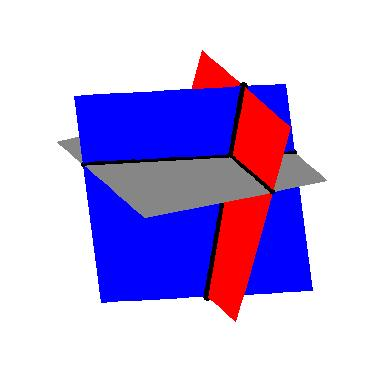
\includegraphics[width=3in]{./LinSystemsGraphics/3planes01.jpg}}

Since the geometry for equations involving more than two variables is complicated, we will focus our efforts on the algebra.  Returning to the system 

\[ \left\{ \begin{array}{rcr} x-\frac{1}{3}y+\frac{1}{2}z  & = & 1 \\ [3pt]
y - \frac{1}{2} z & = & 4 \\ [3pt]
z & = & -1 \\ \end{array} \right.\] 

we note the reason it was so easy to solve is because of its structure.  The third equation is solved for $z$ and the second equation involves only $y$ and $z$. Since the coefficient of $y$ is $1$, it makes it easy to solve for $y$ using our known value for $z$.  Lastly, the coefficient of  $x$ in the first equation is $1$ making it easy to substitute the known values of $y$ and $z$ and then solve for $x$.  

We formalize this pattern below for the most general systems of linear equations.  Again, we use subscripted variables to describe the general case.  The variable with the smallest subscript in a given equation is typically called the \index{system of equations ! leading variable} \textit{leading variable} of that equation.

\smallskip
\colorbox{ResultColor}{\bbm  \begin{definition} \label{systemtriangularform} A system of linear equations with variables $x_{\mbox{\tiny$1$}}$, $x_{\mbox{\tiny$2$}}$, \ldots $x_{n}$ is said to be in \index{system of equations ! triangular form} \index{triangular form} \textbf{triangular form} provided all of the following conditions hold:

\begin{enumerate}

\item  The subscripts of the variables in each equation are always increasing from left to right.

\item  The leading variable in each equation has coefficient $1$.

\item  The subscript on the leading variable in a given equation is greater than the subscript on the leading variable in the equation above it.

\item  Any equation without variables\footnote{necessarily an identity or contradiction} cannot be placed above an equation with variables.

\end{enumerate}

\end{definition}

\ebm}

\smallskip

In our previous system, if we make the obvious choices $x = x_{\mbox{\tiny$1$}}$, $y = x_{\mbox{\tiny$2$}}$, and $z = x_{\mbox{\tiny$3$}}$, we see that the system is in triangular form.\footnote{If letters are used instead of subscripted variables, Definition \ref{systemtriangularform} can be suitably modified using alphabetical order of the variables instead of numerical order on the subscripts of the variables.}   An example of a more complicated system in triangular form is

\[ \left\{ \begin{array}{rcr} x_{\mbox{\tiny$1$}} - 4x_{\mbox{\tiny$3$}} + x_{\mbox{\tiny$4$}} - x_{\mbox{\tiny$6$}} & = & 6 \\ x_{\mbox{\tiny$2$}} + 2x_{\mbox{\tiny$3$}} & = & 1 \\ x_{\mbox{\tiny$4$}} + 3x_{\mbox{\tiny$5$}} - x_{\mbox{\tiny$6$}} & = & 8 \\ x_{\mbox{\tiny$5$}} + 9x_{\mbox{\tiny$6$}} & = & 10 \end{array} \right.\]

Our goal henceforth will be to transform a given system of linear equations into triangular form using the moves in Theorem \ref{equationmoves}.

\begin{example} \label{GaussEqnEx} Use Theorem \ref{equationmoves} to put the following systems into triangular form and then solve the system if possible.  Classify each system as consistent independent, consistent dependent, or inconsistent.\footnote{See Section \ref{AppLinearSystems} for a review of these terms.}

\begin{multicols}{3}

\begin{enumerate}

\item  $\left\{ \begin{array}{rcr} 3x-y+z & = & 3 \\ 2x-4y+3z & = & 16 \\ x-y+z & = & 5 \\ \end{array} \right.$

\item  $\left\{ \begin{array}{rcr} 2x+3y-z & = & 1 \\ 10x-z & = & 2 \\ 4x-9y+2z & = & 5 \\ \end{array} \right.$

\item  $\left\{ \begin{array}{rcr} 3x_{\mbox{\tiny$1$}} +x_{\mbox{\tiny$2$}} + x_{\mbox{\tiny$4$}} & = & 6 \\ 2x_{\mbox{\tiny$1$}} + x_{\mbox{\tiny$2$}} -x_{\mbox{\tiny$3$}}  & = & 4  \\  x_{\mbox{\tiny$2$}} -3x_{\mbox{\tiny$3$}} -2x_{\mbox{\tiny$4$}} & = & 0 \end{array} \right.$

\end{enumerate}

\end{multicols}

{\bf Solution.}  For definitiveness, we label the topmost equation in each system $E1$, the equation beneath that $E2$, and so forth. 

\begin{enumerate}

\item We put the system in triangular form using an algorithm known as \index{system of equations ! Gaussian Elimination}\index{Gaussian Elimination} \textit{Gaussian Elimination}.  Starting with $x$, we transform the system so that conditions 2 and 3 in Definition \ref{systemtriangularform} are satisfied.  Then we move on to the next variable, in this case $y$, and repeat.  

Since the variables in all of the equations have a consistent ordering from left to right, our first move is to get an $x$ in $E1$'s spot with a coefficient of $1$.  While there are many ways to do this, the easiest is to apply the first move listed in Theorem \ref{equationmoves} and interchange $E1$ and $E3$.

\[\begin{array}{ccc}

\left\{  \begin{array}{lrcr}

(E1) & 3x-y+z & = & 3 \\
(E2)  & 2x-4y+3z & = & 16 \\
(E3)  &  x-y+z & = & 5 \\ 

\end{array} \right.

&
\xrightarrow{\text{Switch $E1$ and $E3$}}

&

\left\{ \begin{array}{lrcr}

(E1) & x-y+z & = & 5 \\
(E2) & 2x-4y+3z & = & 16 \\
(E3) & 3x-y+z & = & 3 \\

\end{array} \right.

\end{array}\]



To satisfy Definition \ref{systemtriangularform}, we need to eliminate the $x$'s from $E2$ and $E3$.  We accomplish this by replacing each of them with a sum of themselves and a multiple of $E1$.  To eliminate the $x$ from $E2$, we need to multiply $E1$ by $-2$ then add;  to eliminate the $x$ from $E3$, we need to multiply $E1$ by $-3$ then add.  Applying the third move listed in Theorem \ref{equationmoves} twice, we get

\[ \begin{array}{ccc}

\left\{ 

\begin{array}{lrcr}

(E1) & x-y+z & = & 5 \\
(E2) & 2x-4y+3z & = & 16 \\
(E3) & 3x-y+z & = & 3 \\

\end{array} 

\right.

&

\xrightarrow[\text{Replace $E3$ with $-3E1 + E3$}]{\text{Replace $E2$ with $-2E1 + E2$}}

&

\left\{ 

\begin{array}{lrcr}

(E1) & x-y+z & = & 5 \\
(E2) & -2y+z & = & 6 \\
(E3) & 2y-2z & = & -12 \\

\end{array} 

\right.

 \end{array} \]

Now we enforce the conditions stated in Definition \ref{systemtriangularform} for the variable $y$.  To that end we need to get the coefficient of $y$ in $E2$ equal to $1$.  We apply the second move listed in Theorem \ref{equationmoves} and replace $E2$ with itself times $-\frac{1}{2}$.

\[\begin{array}{ccc}

\left\{ 

\begin{array}{lrcr}

(E1) & x-y+z & = & 5 \\
(E2) & -2y+z & = & 6 \\
(E3) & 2y-2z & = & -12 \\

\end{array} 

\right.

&
\xrightarrow{\text{Replace $E2$ with $-\frac{1}{2}E2$}}

&

\left\{ 

\begin{array}{lrcr}

(E1) & x-y+z & = & 5 \\
(E2) & y - \frac{1}{2}z & = & -3\\
(E3) & 2y-2z & = & -12 \\

\end{array} 

\right.

\end{array}\]

To eliminate the $y$ in $E3$, we add $-2E2$ to it.

\[\begin{array}{ccc}

\left\{ 

\begin{array}{lrcr}

(E1) & x-y+z & = & 5 \\
(E2) & y - \frac{1}{2}z & = & -3\\
(E3) & 2y-2z & = & -12 \\

\end{array} 

\right.
&
\xrightarrow{\text{Replace $E3$ with $-2E2 + E3$}}

&

\left\{ 

\begin{array}{lrcr}

(E1) & x-y+z & = & 5 \\
(E2) & y - \frac{1}{2}z & = & -3\\
(E3) & -z & = & -6 \\

\end{array} 

\right.
\end{array}\]

Finally, we apply the second move from  Theorem \ref{equationmoves} one last time and multiply $E3$ by $-1$ to satisfy the conditions of Definition \ref{systemtriangularform} for the variable $z$.

\[\begin{array}{ccc}


\left\{ 

\begin{array}{lrcr}

(E1) & x-y+z & = & 5 \\
(E2) & y - \frac{1}{2}z & = & -3\\
(E3) & -z & = & -6 \\

\end{array} 

\right.

&
\xrightarrow{\text{Replace $E3$ with $-1E3$}}

&
\left\{ 

\begin{array}{lrcr}

(E1) & x-y+z & = & 5 \\
(E2) & y - \frac{1}{2}z & = & -3\\
(E3) & z & = & 6 \\

\end{array} 

\right.

\end{array}\]


Substituting  $z=6$ into $E2$ gives $y - 3 = -3$ so that $y = 0$.  With $y=0$ and $z=6$, $E1$ becomes $x - 0 + 6 = 5$, or $x = -1$.  Hence, our solution is $(-1,0,6)$.  We leave it to the reader to check that substituting the respective values for $x$, $y$, and $z$ into the original system results in three identities.  

Since there is a solution to the system, the system is classified as consistent. Since there are no free variables,\footnote{Again, see Section \ref{AppLinearSystems} for a review of this concept, if needed.}  the system is classified as  independent.

\item  Proceeding as above, our first step is to get an equation with $x$ in the $E1$ position with $1$ as its coefficient.  Since there is no easy fix, we multiply $E1$ by $\frac{1}{2}$.


\[\begin{array}{ccc}

\left\{ 

\begin{array}{lrcr}

(E1) & 2x+3y-z & = & 1 \\ 
(E2) & 10x-z & = & 2 \\
(E3) &  4x-9y+2z & = & 5 \\

\end{array} 

\right.

&
\xrightarrow{\text{Replace $E1$ with $\frac{1}{2}E1$}}

&

\left\{ 

\begin{array}{lrcr}

(E1) & x+\frac{3}{2}y-\frac{1}{2}z & = & \frac{1}{2} \\ 
(E2) & 10x-z & = & 2 \\
(E3) &  4x-9y+2z & = & 5 \\

\end{array} 

\right.
\end{array}\]

Now it's time to take care of the $x$'s in $E2$ and $E3$.

\[ \begin{array}{ccc}

\left\{ 

\begin{array}{lrcr}

(E1) & x+\frac{3}{2}y-\frac{1}{2}z & = & \frac{1}{2} \\ 
(E2) & 10x-z & = & 2 \\
(E3) &  4x-9y+2z & = & 5 \\

\end{array} 

\right.
&
\xrightarrow[\text{Replace $E3$ with $-4E1 + E3$}]{\text{Replace $E2$ with $-10E1 + E2$}}

&

\left\{ 

\begin{array}{lrcr}

(E1) & x+\frac{3}{2}y-\frac{1}{2}z & = & \frac{1}{2} \\ 
(E2) & -15y+4z & = & -3 \\
(E3) & -15y+4z & = & 3 \\

\end{array} 

\right.
 \end{array} \]

Our next step is to get the coefficient of $y$ in $E2$ equal to $1$.  To that end, we have

\[\begin{array}{ccc}
\left\{ 

\begin{array}{lrcr}

(E1) & x+\frac{3}{2}y-\frac{1}{2}z & = & \frac{1}{2} \\ [3pt]
(E2) & -15y+4z & = & -3 \\ [3pt]
(E3) & -15y+4z & = & 3 \\

\end{array} 

\right.

&
\xrightarrow{\text{Replace $E2$ with $-\frac{1}{15}E2$}}

&

\left\{ 

\begin{array}{lrcr}

(E1) & x+\frac{3}{2}y-\frac{1}{2}z & = & \frac{1}{2} \\ [3pt]
(E2) & y - \frac{4}{15}z & = & \frac{1}{5} \\ [3pt]
(E3) & -15y+4z & = & 3 \\

\end{array} 

\right.

\end{array}\]


Finally, we rid $E3$ of $y$.

\[\begin{array}{ccc}

\left\{ 

\begin{array}{lrcr}

(E1) & x+\frac{3}{2}y-\frac{1}{2}z & = & \frac{1}{2} \\ [3pt]
(E2) & y - \frac{4}{15}z & = & \frac{1}{5} \\ [3pt]
(E3) & -15y+4z & = & 3 \\

\end{array} 

\right.
&
\xrightarrow{\text{Replace $E3$ with $15E2 + E3$}}

&

\left\{ 

\begin{array}{lrcr}

(E1) & x-y+z & = & 5 \\ [3pt]
(E2) & y - \frac{1}{2}z & = & -3\\ [3pt]
(E3) & 0 & = & 6 \\

\end{array} 

\right.
\end{array}\]

The last equation, $0=6$, is a contradiction so the system has no solution.  According to Theorem \ref{equationmoves}, since this system has no solutions, neither does the original, thus we have an inconsistent system.

\item  For our last system, we begin by multiplying $E1$ by $\frac{1}{3}$ to get a coefficient of $1$ on  $x_{\mbox{\tiny$1$}}$.

\[\begin{array}{ccc}

\left\{ 

\begin{array}{lrcr}

(E1) & 3x_{\mbox{\tiny$1$}} +x_{\mbox{\tiny$2$}} + x_{\mbox{\tiny$4$}} & = & 6 \\   
(E2) & 2x_{\mbox{\tiny$1$}} + x_{\mbox{\tiny$2$}} -x_{\mbox{\tiny$3$}}  & = & 4  \\
(E3) &  x_{\mbox{\tiny$2$}} -3x_{\mbox{\tiny$3$}} -2x_{\mbox{\tiny$4$}} & = & 0 \\

\end{array} 

\right.

&
\xrightarrow{\text{Replace $E1$ with $\frac{1}{3}E1$}}

&

\left\{ 

\begin{array}{lrcr}

(E1) & x_{\mbox{\tiny$1$}} + \frac{1}{3}x_{\mbox{\tiny$2$}} + \frac{1}{3}x_{\mbox{\tiny$4$}} & = & 2 \\  
(E2) & 2x_{\mbox{\tiny$1$}} + x_{\mbox{\tiny$2$}} -x_{\mbox{\tiny$3$}}  & = & 4  \\
(E3) &  x_{\mbox{\tiny$2$}} -3x_{\mbox{\tiny$3$}} -2x_{\mbox{\tiny$4$}} & = & 0 \\

\end{array} 

\right.

\end{array}\]

Next we eliminate $x_{\mbox{\tiny$1$}}$ from $E2$


\[\begin{array}{ccc}

\left\{ 

\begin{array}{lrcr}

(E1) & x_{\mbox{\tiny$1$}} + \frac{1}{3}x_{\mbox{\tiny$2$}} + \frac{1}{3}x_{\mbox{\tiny$4$}} & = & 2 \\  [3pt]
(E2) & 2x_{\mbox{\tiny$1$}} + x_{\mbox{\tiny$2$}} -x_{\mbox{\tiny$3$}}  & = & 4  \\ [3pt]
(E3) &  x_{\mbox{\tiny$2$}} -3x_{\mbox{\tiny$3$}} -2x_{\mbox{\tiny$4$}} & = & 0 \\

\end{array} 

\right.

&

\xrightarrow[\text{with $-2E1 + E2$}]{\text{Replace $E2$}}
&

\left\{ 

\begin{array}{lrcr}

(E1) & x_{\mbox{\tiny$1$}} + \frac{1}{3}x_{\mbox{\tiny$2$}} + \frac{1}{3}x_{\mbox{\tiny$4$}} & = & 2 \\ [3pt]
(E2) &        \frac{1}{3} x_{\mbox{\tiny$2$}} -x_{\mbox{\tiny$3$}} -\frac{2}{3}x_{\mbox{\tiny$4$}} & = & 0  \\ [3pt]
(E3) &  x_{\mbox{\tiny$2$}} -3x_{\mbox{\tiny$3$}} -2x_{\mbox{\tiny$4$}} & = & 0 \\

\end{array} 

\right.

\end{array}\]

We switch $E2$ and $E3$ to get a coefficient of $1$ for $x_{\mbox{\tiny$2$}}$.

\[\begin{array}{ccc}

\left\{ 

\begin{array}{lrcr}

(E1) & x_{\mbox{\tiny$1$}} + \frac{1}{3}x_{\mbox{\tiny$2$}} + \frac{1}{3}x_{\mbox{\tiny$4$}} & = & 2 \\  [3pt]
(E2) &        \frac{1}{3} x_{\mbox{\tiny$2$}} -x_{\mbox{\tiny$3$}} -\frac{2}{3}x_{\mbox{\tiny$4$}} & = & 0  \\ [3pt]
(E3) &  x_{\mbox{\tiny$2$}} -3x_{\mbox{\tiny$3$}} -2x_{\mbox{\tiny$4$}} & = & 0 \\

\end{array} 

\right.

&
\xrightarrow{\text{Switch $E2$ and $E3$}}

&
\left\{ 

\begin{array}{lrcr}

(E1) & x_{\mbox{\tiny$1$}} + \frac{1}{3}x_{\mbox{\tiny$2$}} + \frac{1}{3}x_{\mbox{\tiny$4$}} & = & 2 \\  [3pt]
(E2) &    x_{\mbox{\tiny$2$}} -3x_{\mbox{\tiny$3$}} -2x_{\mbox{\tiny$4$}} & = & 0 \\ [3pt]
(E3) &  \frac{1}{3} x_{\mbox{\tiny$2$}} -x_{\mbox{\tiny$3$}} -\frac{2}{3}x_{\mbox{\tiny$4$}} & = & 0  \\

\end{array} 

\right.\end{array}\]

Finally, we eliminate $x_{\mbox{\tiny$2$}}$ in $E3$.

\[\begin{array}{ccc}
\left\{ 

\begin{array}{lrcr}

(E1) & x_{\mbox{\tiny$1$}} + \frac{1}{3}x_{\mbox{\tiny$2$}} + \frac{1}{3}x_{\mbox{\tiny$4$}} & = & 2 \\  [3pt]
(E2) &    x_{\mbox{\tiny$2$}} -3x_{\mbox{\tiny$3$}} -2x_{\mbox{\tiny$4$}} & = & 0 \\ [3pt]
(E3) &  \frac{1}{3} x_{\mbox{\tiny$2$}} -x_{\mbox{\tiny$3$}} -\frac{2}{3}x_{\mbox{\tiny$4$}} & = & 0  \\

\end{array} 

\right.

&

\xrightarrow[\text{with $-\frac{1}{3}E2 + E3$}]{\text{Replace $E3$} }

&

\left\{ 

\begin{array}{lrcr}

(E1) & x_{\mbox{\tiny$1$}} + \frac{1}{3}x_{\mbox{\tiny$2$}} + \frac{1}{3}x_{\mbox{\tiny$4$}} & = & 2 \\  [3pt]
(E2) &    x_{\mbox{\tiny$2$}} -3x_{\mbox{\tiny$3$}} -2x_{\mbox{\tiny$4$}} & = & 0 \\    [3pt]
(E3) & 0 & = & 0  \\

\end{array} 

\right.\end{array}\]

Equation $E3$ reduces to $0=0$,which is always true.  Since we have no equations with $x_{\mbox{\tiny$3$}}$ or $x_{\mbox{\tiny$4$}}$ as leading variables, they are both `free' variables so we have a consistent dependent system.  

We `parametrize' the solution set by letting $x_{\mbox{\tiny$3$}} = s$ and $x_{\mbox{\tiny$4$}} = t$.  From $E2$, we get $x_{\mbox{\tiny$2$}} =  3s + 2t$.  Substituting this and $x_{\mbox{\tiny$4$}} = t$ into $E1$, we have $x_{\mbox{\tiny$1$}} + \frac{1}{3}\left( 3s+2t \right) + \frac{1}{3}t = 2$ which gives $x_{\mbox{\tiny$1$}} = 2 - s - t$.  Our solution is the set $\{ (2-s-t,2s+3t,s,t) \, | \, -\infty < s, t < \infty\}$.\footnote{Here, any choice of $s$ and $t$ determines a point in $4$-dimensional space.  Yeah, we have trouble visualizing that, too.}  We leave it to the reader to verify that the substitutions $x_{1} = 2-s-t$, $x_{2} = 3s+2t$, $x_{3} = s$ and $x_{4} = t$ satisfy the equations in the original system regardless of the choices made for the parameters $s$ and $t$. \qed

\end{enumerate}
\end{example}

Like all algorithms, Gaussian Elimination has the advantage of always producing what we need, but it can also be inefficient at times. For example, when solving the second system in Example \ref{GaussEqnEx}, it is clear after we eliminated the $x$'s in the second step to get the system
 
\[ \left\{ \begin{array}{lrcr} (E1) & x+\frac{3}{2}y-\frac{1}{2}z & = & \frac{1}{2} \\ [3pt]
(E2) & -15y+4z & = & -3 \\ [3pt]
(E3) & -15y+4z & = & 3 \\ \end{array}  \right.\] 

that equations $E2$ and $E3$,  taken together,  produce a contradiction. (We have identical left hand sides and different right hand sides.)  However, the algorithm takes an additional two steps to reach this conclusion.  

We also note that substitution in Gaussian Elimination is delayed until all the elimination is done, whence the name \index{system of equations ! back-substitution} \index{back substitution} \textit{back-substitution}.  This may also be inefficient in many cases.

Lastly, we note that the last system in Example \ref{GaussEqnEx} is underdetermined,\footnote{Recall this means we have fewer equations than unknowns.}  and as it is consistent, we necessarily have free variables in our answer.  We close this section with a standard `mixture' type application of systems of linear equations which features an application of a consistent dependent system.

\begin{example} \label{lucasmixex} Lucas needs to create a $500$ milliliters (mL) of a $40 \%$ acid solution.  He has stock solutions of $30 \%$ and $90 \%$ acid as well as all of the distilled water he wants. Set-up and solve a system of linear equations which determines all of the possible combinations of the stock solutions and water which would produce the required solution.

\smallskip

{ \bf Solution.}  We are after three unknowns, the amount (in mL) of the $30 \%$ stock solution (which we'll call $x$), the amount (in mL) of the $90 \%$ stock solution (which we'll call $y$) and the amount (in mL) of water (which we'll call $w$). We now need to determine some relationships between these variables.  

Our goal is to produce $500$ milliliters of a $40 \%$ acid solution.  This product has two defining characteristics.  First, it must be $500$ mL;  second, it must be $40 \%$ acid.  We take each of these qualities in turn.  

First, the total volume of $500$ mL must be the sum of the volumes of the two stock solutions and the water: \[ \mbox{amount of  $30 \%$ stock solution} + \mbox{amount of  $90 \%$ stock solution} + \mbox{amount of water} = 500 \, \mbox{mL}\] Using our defined variables, this reduces to $x+y+w = 500$.  

Next, we need to make sure the final solution is $40 \%$ acid.   Since water contains no acid, the acid will come from the stock solutions only.  We find $40 \%$ of $500$ mL to be $200$ mL which means the final solution must contain $200$ mL of acid.  We have \[ \mbox{amount of  acid in $30 \%$ stock solution} + \mbox{amount of acid $90 \%$ stock solution}  = 200 \, \mbox{mL}\]  The amount of acid in  $x$ mL of $30 \%$ stock is $0.30x$ and the amount of acid in $y$ mL of $90 \%$ solution is $0.90y$.  We have $0.30x + 0.90y = 200$.  Converting to fractions,\footnote{We do this only because we believe students can use all of the practice with fractions they can get!} our system of equations becomes 

\[ \left\{ \begin{array}{rcl} x+y+w & = & 500 \\ 
\frac{3}{10}x + \frac{9}{10}y & = & 200 \\ \end{array} \right.\]  

We first eliminate the $x$ from the second equation 

\[\begin{array}{ccc}
\left\{ 

\begin{array}{lrcr}

(E1) & x+y+w & = & 500 \\  
(E2) & \frac{3}{10}x + \frac{9}{10}y & = & 200 \\    

\end{array} 

\right.

&

\xrightarrow{\text{Replace $E2$ with $-\frac{3}{10}E1 + E2$}}

&

\left\{ 

\begin{array}{lrcr}

(E1) & x+y+w & = & 500 \\  
(E2) &  \frac{3}{5}y - \frac{3}{10}w & = & 50 \\    

\end{array} 

\right.

\end{array}\]

Next, we get a coefficient of $1$ on the leading variable in $E2$

\[\begin{array}{ccc}


\left\{ 

\begin{array}{lrcr}

(E1) & x+y+w & = & 500 \\  
(E2) &  \frac{3}{5}y - \frac{3}{10}w & = & 50 \\    

\end{array} 

\right.

&

\xrightarrow{\text{Replace $E2$ with $\frac{5}{3}E2$}}

&


\left\{ 

\begin{array}{lrcr}

(E1) & x+y+w & = & 500 \\  
(E2) &  y - \frac{1}{2}w & = & \frac{250}{3} \\    

\end{array} 

\right.
\end{array}\]

Notice that we have no equation to determine $w$, and as such, $w$ is free.  Setting $w = t$ in $E2$, we get $y = \frac{1}{2} t + \frac{250}{3}$.  Substituting for $w$ and $y$ in $E1$ gives $x + \left(\frac{1}{2} t + \frac{250}{3}\right) + t = 500$ so that $x = -\frac{3}{2} t + \frac{1250}{3}$.  

This system is consistent, dependent and its solution set is $\{ \left(-\frac{3}{2} t + \frac{1250}{3}, \frac{1}{2} t + \frac{250}{3}, t\right) \, | \, - \infty < t < \infty\}$.  

While this answer checks algebraically, we have neglected to take into account that $x$, $y$ and $w$, being amounts of acid and water, need to be nonnegative.  That is, $x \geq 0$, $y \geq 0$ and $w \geq 0$.  

The constraint $x \geq 0$ gives us  $-\frac{3}{2} t + \frac{1250}{3} \geq 0$, or $t \leq \frac{2500}{9}$. From $y \geq 0$, we get $\frac{1}{2} t + \frac{250}{3} \geq 0$ or $t \geq -\frac{500}{3}$.  The condition $z \geq 0$ yields $t \geq 0$, and we see that when we take the set theoretic intersection of these intervals, we get $0 \leq t \leq \frac{2500}{9}$.  This gives our final answer is $\{ \left(-\frac{3}{2} t + \frac{1250}{3}, \frac{1}{2} t + \frac{250}{3}, t\right) \, | \,0 \leq t \leq \frac{2500}{9} \}$.  

Of what practical use is our answer?  Suppose there is only $100$ mL of the $90 \%$ solution remaining and it is due to expire.  Can we use all of it to make our required solution?  We would have $y = 100$ so that $\frac{1}{2} t + \frac{250}{3} = 100$, and we get $t = \frac{100}{3}$.  This means the amount of $30 \%$ solution required is $x = -\frac{3}{2} t + \frac{1250}{3} =  -\frac{3}{2} \left(\frac{100}{3}\right) + \frac{1250}{3} = \frac{1100}{3}$ mL, and for the water, $w = t = \frac{100}{3}$ mL.  The reader is invited to check that mixing these three amounts of our constituent solutions produces the required $40 \%$ acid mix.  \qed

\end{example}

\newpage

\subsection{Exercises}

%% SKIPPED %% \documentclass{ximera}

\begin{document}
	\author{Stitz-Zeager}
	\xmtitle{TITLE}


\label{ExercisesforLinSystems}

In Exercises \ref{triangfirst} - \ref{trianglast}, put each system of linear equations into triangular form and solve the system if possible.  Classify each system as consistent independent, consistent dependent, or inconsistent.

\begin{multicols}{2}
\begin{enumerate}


\item $\left\{ \begin{array}{rcr} -5x + y & = & 17  \\ x + y & = & 5  \end{array} \right.$ \label{triangfirst}
\item $\left\{ \begin{array}{rcr} x + y + z & = & 3 \\ 2x - y + z & = & 0 \\ -3x + 5y + 7z & = & 7  \end{array} \right.$

\setcounter{HW}{\value{enumi}}
\end{enumerate}
\end{multicols}



\begin{multicols}{2}
\begin{enumerate}
\setcounter{enumi}{\value{HW}}


\item \label{dependentsystemmuliple} $\left\{ \begin{array}{rcr} 4x - y + z & = & 5 \\ 2y + 6z & = & 30 \\ x + z & = & 5  \end{array} \right.$
\item $\left\{ \begin{array}{rcr} 4x - y + z & = & 5 \\ 2y + 6z & = & 30 \\ x + z & = & 6  \end{array} \right.$

\setcounter{HW}{\value{enumi}}
\end{enumerate}
\end{multicols}



\begin{multicols}{2}
\begin{enumerate}
\setcounter{enumi}{\value{HW}}

\item $\left\{ \begin{array}{rcr} x + y + z & = & -17  \\ y - 3z & = & 0  \end{array} \right.$


\item $\left\{ \begin{array}{rcr} x-2y+3z & = & 7 \\ -3x+y+2z & = & -5 \\ 2x+2y+z & = & 3  \end{array} \right.$


\setcounter{HW}{\value{enumi}}
\end{enumerate}
\end{multicols}



\begin{multicols}{2}
\begin{enumerate}
\setcounter{enumi}{\value{HW}}


\item $\left\{ \begin{array}{rcr} 3x-2y+z & = & -5 \\ x+3y-z & = & 12 \\ x+y+2z & = & 0  \end{array} \right.$
\item $\left\{ \begin{array}{rcr} 2x-y+z& = & -1 \\ 4x+3y+5z & = & 1 \\  5y+3z & = & 4 \end{array} \right.$


\setcounter{HW}{\value{enumi}}
\end{enumerate}
\end{multicols}



\begin{multicols}{2}
\begin{enumerate}
\setcounter{enumi}{\value{HW}}


\item $\left\{ \begin{array}{rcr} x-y+z & = & -4 \\ -3x+2y+4z & = & -5 \\ x-5y+2z & = & -18  \end{array} \right.$
\item $\left\{ \begin{array}{rcr} 2x-4y+z & = & -7 \\ x-2y+2z & = & -2 \\ -x+4y-2z & = & 3  \end{array} \right.$


\setcounter{HW}{\value{enumi}}
\end{enumerate}
\end{multicols}



\begin{multicols}{2}
\begin{enumerate}
\setcounter{enumi}{\value{HW}}


\item $\left\{ \begin{array}{rcr} 2x-y+z & = & 1 \\ 2x+2y-z & = & 1 \\ 3x+6y+4z & = & 9  \end{array} \right.$
\item $\left\{ \begin{array}{rcr} x-3y-4z & = & 3 \\ 3x+4y-z & = & 13 \\ 2x-19y-19z & = & 2  \end{array} \right.$


\setcounter{HW}{\value{enumi}}
\end{enumerate}
\end{multicols}



\begin{multicols}{2}
\begin{enumerate}
\setcounter{enumi}{\value{HW}}


\item $\left\{ \begin{array}{rcr} x+y+z & = & 4 \\ 2x-4y-z& = & -1 \\ x-y & = & 2 \end{array} \right.$
\item $\left\{ \begin{array}{rcr} x-y+z & = & 8 \\ 3x+3y-9z & = & -6 \\  7x-2y+5z & = & 39 \end{array} \right.$


\setcounter{HW}{\value{enumi}}
\end{enumerate}
\end{multicols}



\begin{multicols}{2}
\begin{enumerate}
\setcounter{enumi}{\value{HW}}


\item $\left\{ \begin{array}{rcr} 2x-3y+z & = & -1 \\ 4x-4y+4z & = & -13 \\ 6x-5y+7z & = & -25  \end{array} \right.$

\item  $\left\{ \begin{array}{rcr} 2x_{\mbox{\tiny$1$}} + x_{\mbox{\tiny$2$}} - 12x_{\mbox{\tiny$3$}} -  x_{\mbox{\tiny$4$}} & = & 16 \\ 
-x_{\mbox{\tiny$1$}} + x_{\mbox{\tiny$2$}} + 12x_{\mbox{\tiny$3$}} - 4x_{\mbox{\tiny$4$}} & = & -5  \\  
3x_{\mbox{\tiny$1$}} +  2x_{\mbox{\tiny$2$}} - 16x_{\mbox{\tiny$3$}} - 3x_{\mbox{\tiny$4$}} & = & 25 \\
x_{\mbox{\tiny$1$}} +  2x_{\mbox{\tiny$2$}} - 5x_{\mbox{\tiny$4$}} & = & 11  \end{array} \right.$

\setcounter{HW}{\value{enumi}}
\end{enumerate}
\end{multicols}

\begin{multicols}{2}
\begin{enumerate}
\setcounter{enumi}{\value{HW}}



\item  $\left\{ \begin{array}{rcr} x_{\mbox{\tiny$1$}} - x_{\mbox{\tiny$3$}} & = & -2 \\ 
2x_{\mbox{\tiny$2$}} - x_{\mbox{\tiny$4$}} & = & 0  \\  
x_{\mbox{\tiny$1$}} -  2x_{\mbox{\tiny$2$}} + x_{\mbox{\tiny$3$}} & = & 0 \\
-x_{\mbox{\tiny$3$}} + x_{\mbox{\tiny$4$}} & = & 1  \end{array} \right.$

\item  $\left\{ \begin{array}{rcr} x_{\mbox{\tiny$1$}} - x_{\mbox{\tiny$2$}} - 5x_{\mbox{\tiny$3$}} +  3x_{\mbox{\tiny$4$}} & = & -1 \\ 
x_{\mbox{\tiny$1$}} + x_{\mbox{\tiny$2$}} + 5x_{\mbox{\tiny$3$}} - 3x_{\mbox{\tiny$4$}} & = & 0  \\  
x_{\mbox{\tiny$2$}} + 5x_{\mbox{\tiny$3$}} - 3x_{\mbox{\tiny$4$}} & = & 1 \\
x_{\mbox{\tiny$1$}} -  2x_{\mbox{\tiny$2$}} - 10x_{\mbox{\tiny$3$}} + 6x_{\mbox{\tiny$4$}} & = & -1  \end{array} \right.$ \label{trianglast}

\setcounter{HW}{\value{enumi}}
\end{enumerate}
\end{multicols}


\begin{enumerate}
\setcounter{enumi}{\value{HW}}

\item Find two other forms of the parametric solution to Exercise \ref{dependentsystemmuliple} above by reorganizing the equations so that $x$ or $y$ can be the free variable.

\item \label{herbalteablend} At The Crispy Critter's Head Shop and Patchouli Emporium along with their dried up weeds, sunflower seeds and astrological postcards they sell an herbal tea blend.  By weight, Type I herbal tea is 30\% peppermint, 40\% rose hips and 30\% chamomile, Type II has percents 40\%, 20\% and 40\%, respectively, and Type III has percents 35\%, 30\% and 35\%, respectively.  How much of each Type of tea is needed to make 2 pounds of a new blend of tea that is equal parts peppermint, rose hips and chamomile?  

\item Discuss with your classmates how you would approach Exercise \ref{herbalteablend} above if they needed to use up a pound of Type I tea to make room on the shelf for a new canister.

\item If you were to try to make 100 mL of a $60\%$ acid solution using stock solutions at $20\%$ and $40\%$, respectively, what would the triangular form of the resulting system look like?  Explain.

\end{enumerate}

\newpage

\subsection{Answers}


Because triangular form is not unique, we give only one possible answer to that part of the question.  Yours may be different and still be correct.

\begin{enumerate}

\begin{multicols}{2} \raggedcolumns

\item $\left\{ \begin{array}{rcr} x + y & = & 5  \\ y & = & 7  \end{array} \right.$ 

Consistent independent\\
Solution $(-2, 7)$

\end{multicols}

\begin{multicols}{2} \raggedcolumns

\item $\left\{ \begin{array}{rcr} x - \frac{5}{3}y - \frac{7}{3}z & = & -\frac{7}{3} \\ [3pt] y + \frac{5}{4}z & = & 2 \\ z & = & 0  \end{array} \right.$

Consistent independent\\
Solution $(1, 2, 0)$

\end{multicols}

\begin{multicols}{2} \raggedcolumns

\item $\left\{ \begin{array}{rcr} x - \frac{1}{4}y + \frac{1}{4}z & = & \frac{5}{4} \\ [3pt] y + 3z & = & 15 \\ 0 & = & 0  \end{array} \right.$

Consistent dependent\\
Solution $(-t + 5, -3t + 15, t)$\\
for all real numbers $t$

\end{multicols}

\begin{multicols}{2} \raggedcolumns

\item $\left\{ \begin{array}{rcr} x - \frac{1}{4}y + \frac{1}{4}z & = & \frac{5}{4} \\ [3pt] y + 3z & = & 15 \\ 0 & = & 1 \end{array} \right.$

Inconsistent\\
No solution

\end{multicols}

\begin{multicols}{2} \raggedcolumns

\item $\left\{ \begin{array}{rcr} x + y + z & = & -17  \\ y - 3z & = & 0  \end{array} \right.$
\vspace{.25in}

Consistent dependent\\
Solution $(-4t - 17, 3t, t)$\\
for all real numbers $t$

\end{multicols}

\begin{multicols}{2} \raggedcolumns
\item $\left\{ \begin{array}{rcr} x-2y+3z & = & 7  \\ y - \frac{11}{5}z & = & -\frac{16}{5} \\ z & = & 1 \\  \end{array} \right.$
\vspace{.25in}

Consistent independent\\
Solution $(2,-1,1)$

\end{multicols}

\begin{multicols}{2} \raggedcolumns
\item $\left\{ \begin{array}{rcr} x+y+2z & = & 0  \\ y - \frac{3}{2}z & = & 6 \\ z & = & -2 \\  \end{array} \right.$
\vspace{.25in}

Consistent independent\\
Solution $(1,3,-2)$

\end{multicols}


\begin{multicols}{2} \raggedcolumns
\item $\left\{ \begin{array}{rcr} x - \frac{1}{2} y + \frac{1}{2} z & = & -\frac{1}{2}  \\ [3pt] y + \frac{3}{5} z & = & \frac{3}{5} \\ 0 & = & 1 \\  \end{array} \right.$
\vspace{.25in}

Inconsistent\\
no solution


\end{multicols}


\begin{multicols}{2} \raggedcolumns
\item $\left\{ \begin{array}{rcr} x-y+z & = & -4  \\ y - 7z & = & 17 \\ z & = & -2 \\  \end{array} \right.$
\vspace{.25in}

Consistent independent\\
Solution $(1,3,-2)$

\end{multicols}

\begin{multicols}{2} \raggedcolumns
\item $\left\{ \begin{array}{rcr} x-2y+2z & = & -2  \\ y  & = & \frac{1}{2} \\ z & = & 1 \\  \end{array} \right.$
\vspace{.25in}

Consistent independent\\
Solution $\left(-3,\frac{1}{2},1\right)$

\end{multicols}

\begin{multicols}{2} \raggedcolumns
\item $\left\{ \begin{array}{rcr} x-\frac{1}{2} y+\frac{1}{2} z & = & \frac{1}{2}  \\ [3pt] y - \frac{2}{3} z & = & 0 \\ z & = & 1 \\  \end{array} \right.$
\vspace{.25in}

Consistent independent\\
Solution $\left(\frac{1}{3},\frac{2}{3},1\right)$

\end{multicols}


\begin{multicols}{2} \raggedcolumns
\item $\left\{ \begin{array}{rcr} x-3y-4z & = & 3  \\ y + \frac{11}{13} z & = & \frac{4}{13} \\ 0 & = & 0 \\  \end{array} \right.$
\vspace{.25in}

Consistent dependent\\
Solution $\left(\frac{19}{13} t + \frac{51}{13},-\frac{11}{13} t+\frac{4}{13},t\right)$\\
for all real numbers $t$

\end{multicols}

\begin{multicols}{2} \raggedcolumns
\item $\left\{ \begin{array}{rcr} x+y+z & = & 4  \\ y + \frac{1}{2} z & = & \frac{3}{2} \\ 0 & = & 1 \\  \end{array} \right.$
\vspace{.25in}

Inconsistent\\
no solution


\end{multicols}

\begin{multicols}{2} \raggedcolumns
\item $\left\{ \begin{array}{rcr} x-  y +  z & = & 8  \\ y -2z & = & -5 \\ z & = & 1 \\  \end{array} \right.$
\vspace{.25in}

Consistent independent\\
Solution $\left(4,-3,1\right)$


\end{multicols}


\begin{multicols}{2} \raggedcolumns
\item $\left\{ \begin{array}{rcr} x- \frac{3}{2} y + \frac{1}{2} z & = & -\frac{1}{2}  \\[3pt] y +  z & = & -\frac{11}{2} \\ 0 & = & 0 \\  \end{array} \right.$
\vspace{.25in}

Consistent dependent\\
Solution $\left(-2t - \frac{35}{4},-t - \frac{11}{2},t\right)$\\
for all real numbers $t$

\end{multicols}


\begin{multicols}{2} \raggedcolumns

\item  $\left\{ \begin{array}{rcr} x_{\mbox{\tiny$1$}} + \frac{2}{3}x_{\mbox{\tiny$2$}} - \frac{16}{3}x_{\mbox{\tiny$3$}} -  x_{\mbox{\tiny$4$}} & = & \frac{25}{3} \\ [3pt]
x_{\mbox{\tiny$2$}} + 4x_{\mbox{\tiny$3$}} - 3x_{\mbox{\tiny$4$}} & = & 2  \\  
0 & = & 0 \\
0 & = & 0  \end{array} \right.$

Consistent dependent\\
Solution $(8s - t + 7, -4s + 3t + 2, s, t)$\\
for all real numbers $s$ and $t$

\end{multicols}

\begin{multicols}{2} \raggedcolumns

\item  $\left\{ \begin{array}{rcr} x_{\mbox{\tiny$1$}} - x_{\mbox{\tiny$3$}} & = & -2 \\ [3pt]
x_{\mbox{\tiny$2$}} - \frac{1}{2}x_{\mbox{\tiny$4$}} & = & 0  \\ [3pt]
x_{\mbox{\tiny$3$}} - \frac{1}{2} x_{\mbox{\tiny$4$}} & = & 1 \\ [3pt]
x_{\mbox{\tiny$4$}} & = & 4  \end{array} \right.$

Consistent independent\\
Solution $(1, 2, 3, 4)$

\end{multicols}

\begin{multicols}{2} \raggedcolumns

\item  $\left\{ \begin{array}{rcr} x_{\mbox{\tiny$1$}} - x_{\mbox{\tiny$2$}} - 5x_{\mbox{\tiny$3$}} +  3x_{\mbox{\tiny$4$}} & = & -1 \\ 
x_{\mbox{\tiny$2$}} + 5x_{\mbox{\tiny$3$}} - 3x_{\mbox{\tiny$4$}} & = & \frac{1}{2}  \\  
0 & = & 1 \\
0 & = & 0 \end{array} \right.$

Inconsistent\\
No solution

\end{multicols}

\item If $x$ is the free variable then the solution is $(t, 3t, -t + 5)$ and if $y$ is the free variable then the solution is $\left(\frac{1}{3}t, t, -\frac{1}{3}t + 5\right)$.


\item $\frac{4}{3}- \frac{1}{2}t$ pounds of Type I, $\frac{2}{3} - \frac{1}{2}t$ pounds of Type II and $t$ pounds of Type III where $0 \leq t \leq \frac{4}{3}$.

\end{enumerate}

\end{document}


\closegraphsfile

\end{document}


\newpage

\section{Systems of Linear Equations: Augmented Matrices}

\mfpicnumber{1}

\opengraphsfile{AugMatrices}

\setcounter{footnote}{0}

\label{AugMatrices}

\setlength{\extrarowheight}{0pt}

In Section \ref{LinSystems} we introduced Gaussian Elimination as a means of transforming a system of linear equations into triangular form with the ultimate goal of producing an equivalent system of linear equations which is easier to solve.  If we take a step back and study the process, we see that all of our moves are determined entirely by the \textit{coefficients} of the variables involved, and not the variables themselves.  Much the same thing happened when we studied long division in Section \ref{Polydivision}. Just as we developed synthetic division to streamline that process, in this section, we introduce a similar bookkeeping device to help us solve systems of linear equations, the \textit{matrix}. 

A \index{matrix ! definition}\textit{matrix} as a rectangular array of real numbers.  We typically enclose matrices with `square brackets' of the likes of  `$\left[ \right.$' and `$\left. \right]$', and we size matrices by the number of rows and columns they have.  For example, the \index{matrix ! size} \textit{size} (sometimes called the \index{matrix ! dimension}\index{dimension ! of a matrix}\textit{dimension}) of 

\[ \left[ \begin{array}{rrr} 3 & 0 & -1 \\ 
2 & -5 & 10 \end{array} \right]\] 

is  $2 \times 3$  because it has $2$ rows and $3$ columns.  The individual numbers in a matrix are called its \index{matrix ! entry} \index{entry ! in a matrix} \textit{entries} and are usually labeled with double subscripts: the first tells which row the element is in and the second tells which column it is in.  The rows are numbered from top to bottom and the columns are numbered from left to right.  Matrices themselves are usually denoted by uppercase letters ($A$, $B$, $C$, etc.) while their entries are usually denoted by the corresponding letter.  So, for instance, if we have 

\[ A = \left[ \begin{array}{rrr} 3 & 0 & -1 \\ 
2 & -5 & 10 \end{array} \right]\] 

then $a_{\mbox{\tiny$11$}} = 3$, $a_{\mbox{\tiny$12$}} = 0$, $a_{\mbox{\tiny$13$}} = -1$, $a_{\mbox{\tiny$21$}} = 2$, $a_{\mbox{\tiny$22$}} = -5$, and $a_{\mbox{\tiny$23$}} = 10$.  We shall explore matrices as mathematical objects with their own algebra in Section \ref{MatArithmetic} and introduce them here solely as a bookkeeping device.  Consider the system of linear equations  from number 2 in Example \ref{GaussEqnEx}

\[\left\{ \begin{array}{lrcr} (E1) & 2x+3y-z & = & 1 \\ 
(E2) & 10x-z & = & 2 \\ 
(E3) & 4x-9y+2z & = & 5 \\ \end{array} \right.\]  

We encode this system into a matrix by assigning each equation to a corresponding row.  Within that row, each variable and the constant gets its own column, and to separate the variables on the left hand side of the equation from the constants on the right hand side, we use a vertical bar, $|$.  Note that in $E2$, since $y$ is not present, we record its coefficient as $0$. The matrix associated with this system is 

\[ \begin{array}{c} \begin{array}{rrrrrrr} & & & \hspace{.33in} x & \hspace{.12in} y & \hspace{.1in} z & \hspace{.03in} c \\ \end{array} \\  \begin{array}{r} (E1) \rightarrow \\ (E2) \rightarrow \\ (E3) \rightarrow \end{array}  \left[ \begin{array}{rrr|r} 2 & 3 & -1 & 1\\ 10 & 0 & -1 & 2 \\ 4 & -9 & 2 & 5 \end{array} \right] \end{array} \]  

This matrix is called an \index{matrix ! augmented}\index{augmented matrix}\textit{augmented matrix} because the column containing the constants is appended to the matrix containing the coefficients.\footnote{We shall study the coefficient and constant matrices separately in Section \ref{MatArithmetic}.}  To solve this system, we can use the same kind operations on the \textit{rows} of the matrix that we performed on the \textit{equations} of the system. More specifically, we have the following analog of Theorem \ref{equationmoves} below.

\smallskip

\colorbox{ResultColor}{\bbm

\begin{thm}  \label{rowops} \textbf{Row Operations:}  Given an augmented matrix for a system of linear equations, the following row operations produce an augmented matrix which corresponds to an equivalent system of linear equations. \index{matrix ! row operations} \index{row operations for a matrix}

\begin{itemize}

\item  Interchange any two rows.

\item  Replace a row with a nonzero multiple of itself.\footnote{That is, the row obtained by multiplying each entry in the row by the same nonzero number.}

\item  Replace a row with itself plus a nonzero multiple of another row.\footnote{Where we add entries in  corresponding columns.}

\end{itemize}

\end{thm}  

\ebm}

\smallskip 

As a demonstration of the moves in Theorem \ref{rowops}, we revisit some of the steps that were used in solving the systems of linear equations in Example \ref{GaussEqnEx} of Section \ref{LinSystems}.  The reader is encouraged to perform the indicated operations on the rows of the augmented matrix to see that the machinations are identical to what is done to the coefficients of the variables in the equations. We first see a demonstration of switching two rows using the first step of part 1 in Example \ref{GaussEqnEx}. 

\[\begin{array}{ccc}

\left\{  \begin{array}{lrcr}

(E1) & 3x-y+z & = & 3 \\
(E2) & 2x-4y+3z & = & 16 \\
(E3)  &  x-y+z & = & 5 \\ 

\end{array} \right.

&
\xrightarrow{\text{Switch $E1$ and $E3$}}

&

\left\{ \begin{array}{lrcr}

(E1) & x-y+z & = & 5 \\
(E2) & 2x-4y+3z & = & 16 \\
(E3) & 3x-y+z & = & 3 \\

\end{array} \right.

\end{array}\]

\[\begin{array}{ccc}

\left[ \begin{array}{rrr|r} 
3 & -1 & \hphantom{-}1 & 3 \\ 
2 & -4 & 3 & 16 \\ 
1 & -1 & 1 & 5  \\
\end{array} \right]

&
\xrightarrow{\text{Switch $R1$ and $R3$}}

&

\left[ \begin{array}{rrr|r} 
1 & -1 & \hphantom{-}1 & 5  \\
2 & -4 & 3 & 16 \\ 
3 & -1 & 1 & 3 \\ 

\end{array} \right]

\end{array}\]

Next, we have a demonstration of replacing a row with a nonzero multiple of itself using the first step of part 3 in Example \ref{GaussEqnEx}.

 \[\begin{array}{ccc}

\left\{ 

\begin{array}{lrcr}

(E1) & 3x_{\mbox{\tiny$1$}} +x_{\mbox{\tiny$2$}} + x_{\mbox{\tiny$4$}} & = & 6 \\   
(E2) & 2x_{\mbox{\tiny$1$}} + x_{\mbox{\tiny$2$}} -x_{\mbox{\tiny$3$}}  & = & 4  \\
(E3) &  x_{\mbox{\tiny$2$}} -3x_{\mbox{\tiny$3$}} -2x_{\mbox{\tiny$4$}} & = & 0 \\

\end{array} 

\right.

&
\xrightarrow{\text{Replace $E1$ with $\frac{1}{3}E1$}}

&

\left\{ 

\begin{array}{lrcr}

(E1) & x_{\mbox{\tiny$1$}} + \frac{1}{3}x_{\mbox{\tiny$2$}} + \frac{1}{3}x_{\mbox{\tiny$4$}} & = & 2 \\  
(E2) & 2x_{\mbox{\tiny$1$}} + x_{\mbox{\tiny$2$}} -x_{\mbox{\tiny$3$}}  & = & 4  \\
(E3) &  x_{\mbox{\tiny$2$}} -3x_{\mbox{\tiny$3$}} -2x_{\mbox{\tiny$4$}} & = & 0 \\

\end{array} 

\right.

\end{array}\]

\[\begin{array}{ccc}

\left[ \begin{array}{rrrr|r} 
3 & \hphantom{-} 1 & 0 & 1 & 6  \\
2 & 1 & -1 & 0 & 4 \\ 
0 & 1 & -3 & -2 & 0 \\ 

\end{array} \right]

&
\xrightarrow{\text{Replace $R1$ with $\frac{1}{3}R1$}}

&

\left[ \begin{array}{rrrr|r} 
1 & \frac{1}{3} & 0 & \frac{1}{3} & 2  \\
2 & \hphantom{-}1 & -1 & 0 & 4 \\ 
0 & 1 & -3 & -2 & 0 \\ 

\end{array} \right]
\end{array}\]

Finally, we have an example of replacing a row with itself plus a multiple of another row using the second step from part 2 in Example \ref{GaussEqnEx}.

\[ \begin{array}{ccc}

\left\{ 

\begin{array}{lrcr}

(E1) & x+\frac{3}{2}y-\frac{1}{2}z & = & \frac{1}{2} \\ 
(E2) & 10x-z & = & 2 \\
(E3) &  4x-9y+2z & = & 5 \\

\end{array} 

\right.
&
\xrightarrow[\text{Replace $E3$ with $-4E1 + E3$}]{\text{Replace $E2$ with $-10E1 + E2$}}

&

\left\{ 

\begin{array}{lrcr}

(E1) & x+\frac{3}{2}y-\frac{1}{2}z & = & \frac{1}{2} \\ 
(E2) & -15y+4z & = & -3 \\
(E3) & -15y+4z & = & 3 \\

\end{array} 

\right.
 \end{array} \]
 
\[\begin{array}{ccc}

\left[ \begin{array}{rrr|r} 
1 & \frac{3}{2} & -\frac{1}{2} & \frac{1}{2}  \\
10 & 0 & -1 & 2 \\ 
4 & -9 & 2 & 5 \\ 

\end{array} \right]

&
\xrightarrow[\text{Replace $R3$ with $-4R1 + R3$}]{\text{Replace $R2$ with $-10R1 + R2$}}
&

\left[ \begin{array}{rrr|r} 
1 & \frac{3}{2} & -\frac{1}{2} & \frac{1}{2}  \\
0 & -15 & 4 & -3 \\ 
0 & -15 & 4 & 3 \\ 

\end{array} \right]

\end{array}\]

The matrix equivalent of `triangular form' is \index{matrix ! row echelon form} \index{row echelon form} \textit{row echelon form}.  The reader is encouraged to refer to Definition \ref{systemtriangularform} for comparison.  Note that the analog of `leading variable' of an equation is `leading entry' of a row.  Specifically, the first nonzero entry (if it exists) in a row is called the  \index{matrix ! leading entry} \textit{leading entry} of that row.
 
\smallskip

\colorbox{ResultColor}{\bbm  

\begin{defn} \label{rowechelonform} A matrix is said to be in \textbf{row echelon form} provided all of the following conditions hold:

\begin{enumerate}

\item  The first nonzero entry in each row is $1$.

\item  The leading $1$ of a given row must be to the right of the leading $1$ of the row above it.

\item  Any row of all zeros cannot be placed above a row with nonzero entries.

\end{enumerate}



\end{defn}

\ebm}

\smallskip

To solve a system of a linear equations using an augmented matrix, we encode the system into an augmented matrix and  apply Gaussian Elimination to the rows to get the matrix into row-echelon form.  We then decode the matrix and back substitute.  The next example illustrates this nicely.

\begin{ex}  \label{GaussExMatrix} Use an augmented matrix to transform the following system of linear equations into triangular form. Solve the system.
\[\left\{ \begin{array}{rcl} 3x  - y  + z & = & 8 \\ x +  2y  -  z & = & 4 \\  2x+ 3y - 4z & = & 10 \\  \end{array} \right.\]

{\bf Solution.}  We first encode the system into an augmented matrix.

\[ \begin{array}{ccc}

\left\{ \begin{array}{rcl} 3x  - y  + z & = & 8 \\ x +  2y  -  z & = & 4 \\  2x+ 3y - 4z & = & 10 \\  \end{array} \right.

&

\xrightarrow{\text{Encode into the matrix}}

&

 \left[ \begin{array}{rrr|r} 3 & -1 & 1 & 8 \\ 1 & 2 & -1 & 4 \\ 2 & 3 & -4 & 10 \\ \end{array} \right]
 
 
 \end{array}\]

Thinking back to Gaussian Elimination at an equations level, our first order of business is to get $x$ in $E1$ with a coefficient of $1$.  At the matrix level, this means getting a leading $1$ in $R1$.  This is in accordance with the first criteria in Definition \ref{rowechelonform}.  To that end, we interchange $R1$ and $R2$.  

\[\begin{array}{ccc}

\left[ \begin{array}{rrr|r} 
3 & -1 & 1 & 8 \\ 
1 & 2 & -1 & 4 \\ 
2 & 3 & -4 & 10 \\ 
\end{array} \right]

& 

\xrightarrow{\text{Switch $R1$ and $R2$}}

&

\left[ \begin{array}{rrr|r}
1 & 2 & -1 & 4 \\  
3 & -1 & 1 & 8 \\ 
2 & 3 & -4 & 10 \\ 
\end{array} \right]


\end{array}\]



Our next step is to eliminate the $x$'s from $E2$ and $E3$.  From a matrix standpoint, this means we need $0$'s below the leading $1$ in $R1$.  This guarantees the leading $1$ in $R2$ will be to the right of the leading $1$ in $R1$ in accordance with the second requirement of Definition \ref{rowechelonform}.

\[\begin{array}{ccc}

\left[ \begin{array}{rrr|r}
1 & 2 & -1 & 4 \\  
3 & -1 & 1 & 8 \\ 
2 & 3 & -4 & 10 \\ 
\end{array} \right]
&
\xrightarrow[\text{Replace $R3$ with $-2R1+R3$}]{\text{Replace $R2$ with $-3R1 +R2$}} 
&
\left[ \begin{array}{rrr|r}  
1 & 2 & -1 & 4 \\  
0 & -7 & 4 & -4 \\ 
0 & -1 & -2  & 2 \\ 
\end{array} \right]



\end{array}\]

Now we repeat the above process for the variable $y$.  That is, we need the leading entry in $R2$ to be $1$.

\[\begin{array}{ccc}

\left[ \begin{array}{rrr|r}  
1 & 2 & -1 & 4 \\  
0 & -7 & 4 & -4 \\ 
0 & -1 & -2  & 2 \\ 
\end{array} \right]  
& 
\xrightarrow{\text{Replace $R2$ with $-\frac{1}{7}R2$}}  
& 
\left[ \begin{array}{rrr|r} 
1 & 2 & -1 & 4 \\ 
0 & 1 & -\frac{4}{7} & \frac{4}{7} \\ 
0 & -1 & -2 & 2 \\
\end{array} \right]

\end{array}\]

To ensure the leading $1$ in $R3$ is to the right of the leading $1$ in $R2$, we get a $0$ in the second column of $R3$.

\[ \begin{array}{ccc}

\left[ \begin{array}{rrr|r} 
1 & 2 & -1 & 4 \\ 
0 & 1 & -\frac{4}{7} & \frac{4}{7} \\ 
0 & -1 & -2 & 2 \\ 
\end{array} \right]  
& 
\xrightarrow{\text{Replace $R3$ with $R2+R3$}} 
&  
\left[ \begin{array}{rrr|r} 
1 & \hphantom{-}2 & -1 & 4 \\ [2pt]
0 & 1 & -\frac{4}{7} & \frac{4}{7} \\ [2pt]
0 & 0 & -\frac{18}{7} & \frac{18}{7} \\ 
\end{array} \right]


\end{array}\]

Finally, we get the leading entry in $R3$ to be $1$.

\[\begin{array}{ccc}

\left[ \begin{array}{rrr|r} 
1 & \hphantom{-}2 & -1 & 4 \\ [2pt]
0 & 1 & -\frac{4}{7} & \frac{4}{7} \\ [2pt]
0 & 0 & -\frac{18}{7} & \frac{18}{7} \\ 
\end{array} \right]   
& 
\xrightarrow{\text{Replace $R3$ with $-\frac{7}{18}R3$}} 
& 
\left[ \begin{array}{rrr|r} 
1 & \hphantom{-}2 & -1 & 4 \\ 
0 & 1 & -\frac{4}{7} & \frac{4}{7} \\ 
0 & 0 &1 & -1 \\ 
\end{array} \right]

\end{array}\]

Decoding from the matrix gives a system in triangular form

\[ \begin{array}{ccc}

\left[ \begin{array}{rrr|r} 
1 & \hphantom{-}2 & -1 & 4 \\ 
0 & 1 & -\frac{4}{7} & \frac{4}{7} \\ 
0 & 0 &1 & -1 \\ 
\end{array} \right]  
& 
\xrightarrow{\text{Decode from the matrix}} 
& 
\left \{ \begin{array}{rcr} 
x + 2y-z & = & 4 \\ 
y - \frac{4}{7} z & = & \frac{4}{7} \\ 
z & = & -1 \end{array} \right.

\end{array}\]

We get $z=-1$,  $y = \frac{4}{7} z + \frac{4}{7} = \frac{4}{7}(-1)+\frac{4}{7} = 0$ and $x = -2y+z+4 = -2(0)+(-1)+4 = 3$ for a final answer of $(3,0,-1)$.  We leave it to the reader to check. \qed

\end{ex}

As part of Gaussian Elimination, we used row operations to obtain $0$'s beneath each leading $1$ to put the matrix into row echelon form.  If we also require that $0$'s are the only numbers above a leading $1$, we have what is known as  the \index{matrix ! reduced row echelon form} \index{reduced row echelon form} \textit{reduced row echelon form} of the matrix.

\smallskip

\colorbox{ResultColor}{\bbm  

\begin{defn} \label{reducedrowechelonform} A matrix is said to be in \textbf{reduced row echelon form} provided both of the following conditions hold:

\begin{enumerate}

\item  The matrix is in row echelon form.

\item The leading $1$s are the only nonzero entry in their respective columns.

\end{enumerate}

\end{defn}

\ebm}

\smallskip

Of what significance is the reduced row echelon form of a matrix?  To illustrate, let's take the row echelon form from Example \ref{GaussExMatrix} and perform the necessary steps to put into reduced row echelon form.  We start by using the leading $1$ in $R3$ to zero out the numbers in the rows above it.

\[ \begin{array}{ccc}

\left[ \begin{array}{rrr|r} 
1 & \hphantom{-}2 & -1 & 4 \\ 
0 & 1 & -\frac{4}{7} & \frac{4}{7} \\ 
0 & 0 &1 & -1 \\ 
\end{array} \right]  
& 
\xrightarrow[\text{Replace $R2$ with $\frac{4}{7} R3 + R2$}]{\text{Replace $R1$ with $R3+R1$}} 
& 
\left[ \begin{array}{rrr|r} 
1 & 2 & 0 & 3 \\ 
0 & 1 & 0 & 0 \\ 
0 & 0 &1 & -1 \\ 
\end{array} \right]  

\end{array}\]

Finally, we take care of the $2$ in $R1$ above the leading $1$ in $R2$.

\[ \begin{array}{ccc}

\left[ \begin{array}{rrr|r} 
1 & 2 & 0 & 3 \\ 
0 & 1 & 0 & 0 \\ 
0 & 0 &1 & -1 \\ 
\end{array} \right]   
& 
\xrightarrow{\text{Replace $R1$ with $-2R2+R1$}}
& 
\left[ \begin{array}{rrr|r} 
1 & 0 & 0 & 3 \\ 
0 & 1 & 0 & 0 \\ 
0 & 0 &1 & -1 \\ 
\end{array} \right]  

\end{array}\]

To our surprise and delight, when we decode this matrix, we obtain the solution instantly without having to deal with any back-substitution at all.

\[ \begin{array}{ccc}

\left[ \begin{array}{rrr|r} 
1 & 0 & 0 & 3 \\ 
0 & 1 & 0 & 0 \\ 
0 & 0 &1 & -1 \\ 
\end{array} \right]  
 
& 
\xrightarrow{\text{Decode from the matrix}} 
& 
\left\{ \begin{array}{rcr} 
x & = & 3 \\ 
y & = & 0 \\ 
z & = & -1 \end{array} \right.

\end{array}\]

Note that in the previous discussion, we could have started with $R2$ and used it to get a zero above its leading $1$ and then done the same for the leading $1$ in $R3$.  By starting with $R3$, however, we get more zeros first, and the more zeros there are, the faster the remaining calculations will be.\footnote{Carl also finds starting with $R3$ to be more symmetric, in a purely poetic way.}  It is also worth noting that while a matrix has several\footnote{infinite, in fact} row echelon forms, it has only one reduced row echelon form.  The process by which we have put a matrix into reduced row echelon form is called \index{system of equations ! Gauss-Jordan Elimination} \index{Gauss-Jordan Elimination} \textit{Gauss-Jordan Elimination}.

\begin{ex}  Solve the following system using an augmented matrix.  Use Gauss-Jordan Elimination to put the augmented matrix into reduced row echelon form.  

\[\left \{ \begin{array}{rcr} 
x_{\mbox{\tiny$2$}} - 3x_{\mbox{\tiny$1$}} + x_{\mbox{\tiny$4$}} & = & 2 \\ 
2x_{\mbox{\tiny$1$}} + 4x_{\mbox{\tiny$3$}} & = & 5 \\ 
4x_{\mbox{\tiny$2$}}-x_{\mbox{\tiny$4$}} & = & 3  \end{array} \right.\]

{\bf Solution.} We first encode the system into a matrix.  (Pay attention to the subscripts!)

\[ \begin{array}{ccc}

\left\{ \begin{array}{rcr} 
x_{\mbox{\tiny$2$}} - 3x_{\mbox{\tiny$1$}} + x_{\mbox{\tiny$4$}} & = & 2 \\ 
2x_{\mbox{\tiny$1$}} + 4x_{\mbox{\tiny$3$}} & = & 5 \\ 
4x_{\mbox{\tiny$2$}}-x_{\mbox{\tiny$4$}} & = & 3  \end{array} \right.

&

\xrightarrow{\text{Encode into the matrix}}

&

 \left[ \begin{array}{rrrr|r}
 -3 & \hphantom{-}1 & \hphantom{-}0 & 1 & 2 \\
 2 & 0 & 4 & 0 & 5 \\
 0 & 4 & 0 & -1 & 3 \\ \end{array} \right]

 \end{array}\]
 
 Next, we get a leading $1$ in the first column of $R1$.

\[ \begin{array}{ccc}

 \left[ \begin{array}{rrrr|r}
 -3 & \hphantom{-}1 & \hphantom{-}0 & 1 & 2 \\
 2 & 0 & 4 & 0 & 5 \\
  0 & 4 & 0 & -1 & 3 \\  \end{array} \right]
&

\xrightarrow{\text{Replace $R1$ with $-\frac{1}{3}R1$}}

&

 \left[ \begin{array}{rrrr|r}
 1 & -\frac{1}{3} & \hphantom{-}0 & -\frac{1}{3} & -\frac{2}{3} \\
 2 & 0 & 4 & 0 & 5 \\
 0 & 4 & 0 & -1 & 3 \\  \end{array} \right]

 \end{array}\]

Now we eliminate the nonzero entry below our leading $1$.

\[ \begin{array}{ccc}

 \left[ \begin{array}{rrrr|r}
 1 & -\frac{1}{3} & \hphantom{-}0 & -\frac{1}{3} & -\frac{2}{3} \\
 2 & 0 & 4 & 0 & 5 \\
  0 & 4 & 0 & -1 & 3 \\  \end{array} \right]
&

\xrightarrow{\text{Replace $R2$ with $-2R1+R2$}}

&

 \left[ \begin{array}{rrrr|r}
 1 & -\frac{1}{3} & \hphantom{-}0 & -\frac{1}{3} & -\frac{2}{3} \\ [2pt]
 0 & \frac{2}{3} & 4 & \frac{2}{3} & \frac{19}{3} \\ [2pt]
 0 & 4 & 0 & -1 & 3 \\  \end{array} \right]

 \end{array}\]

We proceed to get a leading $1$ in $R2$.

\[ \begin{array}{ccc}


 \left[ \begin{array}{rrrr|r}
 1 & -\frac{1}{3} & \hphantom{-}0 & -\frac{1}{3} & -\frac{2}{3} \\ [2pt]
 0 & \frac{2}{3} & 4 & \frac{2}{3} & \frac{19}{3} \\ [2pt]
 0 & 4 & 0 & -1 & 3 \\  \end{array} \right]

&

\xrightarrow{\text{Replace $R2$ with $\frac{3}{2}R2$}}

&

 \left[ \begin{array}{rrrr|r}
 1 & -\frac{1}{3} & \hphantom{-}0 & -\frac{1}{3} & -\frac{2}{3} \\ [2pt]
 0 & 1 & 6 & 1 & \frac{19}{2} \\ [2pt]
 0 & 4 & 0 & -1 & 3 \\  \end{array} \right]

 \end{array}\]
 
We now zero out the entry below the leading $1$ in $R2$.


\[ \begin{array}{ccc}


 \left[ \begin{array}{rrrr|r}
 1 & -\frac{1}{3} & \hphantom{-}0 & -\frac{1}{3} & -\frac{2}{3} \\ [2pt]
 0 & 1 & 6 & 1 & \frac{19}{2} \\ [2pt]
 0 & 4 & 0 & -1 & 3 \\  \end{array} \right]

&

\xrightarrow{\text{Replace $R3$ with $-4R2+R3$}}

&

 \left[ \begin{array}{rrrr|r}
 1 & -\frac{1}{3} & 0 & -\frac{1}{3} & -\frac{2}{3} \\ [2pt]
 0 & 1 & 6 & 1 & \frac{19}{2} \\ [2pt]
 0 & 0& -24 & -5 & -35 \\  \end{array} \right]

 \end{array}\]
 
Next, it's time for a leading $1$ in $R3$.
\[ \begin{array}{ccc}


 \left[ \begin{array}{rrrr|r}
 1 & -\frac{1}{3} & 0 & -\frac{1}{3} & -\frac{2}{3} \\ [2pt]
 0 & 1 & 6 & 1 & \frac{19}{2} \\ [2pt]
 0 & 0& -24 & -5 & -35 \\  \end{array} \right]
&

\xrightarrow{\text{Replace $R3$ with $-\frac{1}{24}R3$}}

&

 \left[ \begin{array}{rrrr|r}
 1 & -\frac{1}{3} & \hphantom{-}0 & -\frac{1}{3} & -\frac{2}{3} \\ [2pt]
 0 & 1 & 6 & 1 & \frac{19}{2} \\ [2pt]
 0 & 0& 1 & \frac{5}{24} & \frac{35}{24} \\  \end{array} \right]

 \end{array}\]
 
The matrix is now in row echelon form.  To get the reduced row echelon form, we start with the last leading $1$ we produced and work to get $0$'s above it.
\[ \begin{array}{ccc}

 \left[ \begin{array}{rrrr|r}
 1 & -\frac{1}{3} & \hphantom{-}0 & -\frac{1}{3} & -\frac{2}{3} \\ [2pt]
 0 & 1 & 6 & 1 & \frac{19}{2} \\ [2pt]
 0 & 0& 1 & \frac{5}{24} & \frac{35}{24} \\  \end{array} \right]&

\xrightarrow{\text{Replace $R2$ with $-6R3+R2$}}

&

 \left[ \begin{array}{rrrr|r}
 1 & -\frac{1}{3} & \hphantom{-}0 & -\frac{1}{3} & -\frac{2}{3} \\ [2pt]
 0 & 1 & 0 & -\frac{1}{4} & \frac{3}{4} \\ [2pt]
 0 & 0& 1 & \frac{5}{24} & \frac{35}{24} \\  \end{array} \right]

 \end{array}\]

Lastly, we get a $0$ above the leading $1$ of $R2$.

\[ \begin{array}{ccc}

 \left[ \begin{array}{rrrr|r}
 1 & -\frac{1}{3} & \hphantom{-}0 & -\frac{1}{3} & -\frac{2}{3} \\ [2pt]
 0 & 1 & 0 & -\frac{1}{4} & \frac{3}{4} \\ [2pt]
 0 & 0& 1 & \frac{5}{24} & \frac{35}{24} \\  \end{array} \right]
 
 &

\xrightarrow{\text{Replace $R1$ with $\frac{1}{3}R2+R1$}}

&

 \left[ \begin{array}{rrrr|r}
 1 & \hphantom{-}0 & \hphantom{-}0 & -\frac{5}{12} & -\frac{5}{12} \\ [2pt]
 0 & 1 & 0 & -\frac{1}{4} & \frac{3}{4} \\ [2pt]
 0 & 0& 1 & \frac{5}{24} & \frac{35}{24} \\  \end{array} \right]

 \end{array}\]
 
 At last, we decode to get
 
 \[ \begin{array}{ccc}

 \left[ \begin{array}{rrrr|r}
 1 & \hphantom{-}0 & \hphantom{-}0 & -\frac{5}{12} & -\frac{5}{12} \\ [2pt]
 0 & 1 & 0 & -\frac{1}{4} & \frac{3}{4} \\ [2pt]
 0 & 0& 1 & \frac{5}{24} & \frac{35}{24} \\  \end{array} \right] 
 
& 
\xrightarrow{\text{Decode from the matrix}} 
& 
\left\{ \begin{array}{rcr} 
x_{\mbox{\tiny$1$}} - \frac{5}{12} x_{\mbox{\tiny$4$}} & = & -\frac{5}{12} \\ [2pt]
x_{\mbox{\tiny$2$}} - \frac{1}{4}x_{\mbox{\tiny$4$}} & = & \frac{3}{4} \\ [2pt]
x_{\mbox{\tiny$3$}} + \frac{5}{24} x_{\mbox{\tiny$4$}} & = & \frac{35}{24} \end{array} \right.

\end{array}\]

We see  $x_{\mbox{\tiny$4$}}$ is free and assign it the parameter $t$.  We obtain $x_{\mbox{\tiny$3$}} = -\frac{5}{24} t + \frac{35}{24}$, $x_{\mbox{\tiny$2$}} = \frac{1}{4} t + \frac{3}{4}$, and $x_{\mbox{\tiny$1$}} = \frac{5}{12}t - \frac{5}{12}$.  Our solution is $\left\{ \left( \frac{5}{12}t - \frac{5}{12}, \frac{1}{4} t + \frac{3}{4}, -\frac{5}{24} t + \frac{35}{24}, t \right) : -\infty < t < \infty \right\}$ which we leave to the reader to check. \qed

\end{ex}

Like all good algorithms, putting a matrix in row echelon or reduced row echelon form can easily be programmed into a calculator, and, doubtless, your graphing calculator has such a feature.  We make use of thus feature in next example to avoid tedious arithmetic.

\begin{ex}  \label{matrixcurvefitting} Find the quadratic function passing through the points $(-1,3)$, $(2,4)$, $(5,-2)$.

\smallskip

{\bf Solution.} According to Definition \ref{quadraticfunction}, a quadratic function has the form $f(x) =ax^2+bx+c$ where $a \neq 0$.   Our goal is to find $a$, $b$ and $c$ so that the three given points are on the graph of $f$.   

Since $(-1,3)$ is on the graph of $f$, we now $f(-1) = 3$.  This gives  $a(-1)^2+b(-1) + c = 3$, or  $a-b+c=3$. This last equation is a linear equation with the variables $a$, $b$ and $c$.  Similarly, if the point  $(2,4)$ is on the graph of $f$, then $f(2) = 4$, so  $4a+2b+c = 4$.  Lastly, the point $(5,-2)$ is on the graph of $f$ gives us $25a+5b+c = -2$.  Putting these together, we obtain a system of three linear equations, which we encode into the matrix below.  
\[ \begin{array}{ccc}

\left\{ \begin{array}{rcr} 
a-b+c & = & 3 \\ 
4a+2b+c & = & 4 \\ 
25a+5b+c & = & -2  \end{array} \right.

&

\xrightarrow{\text{Encode into the matrix}}

&

 \left[ \begin{array}{rrr|r}
1 & -1 & \hphantom{-}1 & 3 \\
 4 & 2 & 1 & 4 \\
 25 & 5 & 1 & -2 \\ \end{array} \right]

 \end{array}\]

Using a calculator,\footnote{We've tortured you enough already with fractions in this exposition!} we find $a = -\frac{7}{18}$, $b = \frac{13}{18}$ and $c = \frac{37}{9}$.  Hence, the one and only quadratic which fits the bill is $f(x) = -\frac{7}{18} x^2 + \frac{13}{18} x + \frac{37}{9}$.  To verify this analytically, we see that $f(-1) = 3$, $f(2) = 4$, and $f(5) = -2$.  We can use the calculator to check our solution as well by plotting the three data points and the function $f$.
\begin{center}

\begin{tabular}{cc}

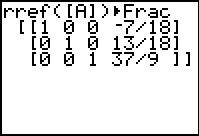
\includegraphics[width=2in]{./AugMatricesGraphics/RREF01.jpg} \hspace{.5in} & 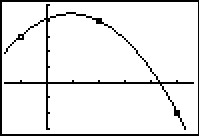
\includegraphics[width=2in]{./AugMatricesGraphics/QUADFIT01.jpg} \\
& The graph of $f(x) = -\frac{7}{18} x^2 + \frac{13}{18} x + \frac{37}{9}$ \\ & with the points $(-1,3)$, $(2,4)$ and $(5,-2)$ \\

\end{tabular}

\end{center}

\qed

\end{ex}

\newpage

\subsection{Exercises}

\label{ExercisesforAugMatrices}

In Exercises \ref{rreffirst} - \ref{rreflast}, state whether the given matrix is in reduced row echelon form, row echelon form only or in neither of those forms.

\begin{multicols}{3} 
\begin{enumerate}


\item $\left[ \begin{array}{rr|r} 
1 & 0 & 3 \\ 
0 & 1 & 3  \\ 
\end{array} \right]$ \label{rreffirst}

\item $\left[ \begin{array}{rrr|r} 
3 & -1 & \hphantom{-}1 & 3 \\ 
2 & -4 & 3 & 16 \\ 
1 & -1 & 1 & 5  \\
\end{array} \right]$

\item $\left[ \begin{array}{rrr|r} 
1 & 1 & 4 & 3 \\ 
0 & 1 & 3 & 6 \\ 
0 & 0 & 0 & 1  \\
\end{array} \right]$

\setcounter{HW}{\value{enumi}}
\end{enumerate}
\end{multicols}

\begin{multicols}{3}
\begin{enumerate}
\setcounter{enumi}{\value{HW}}


\item $\left[ \begin{array}{rrr|r} 
1 & 0 & 0 & 0 \\ 
0 & 1 & 0 & 0 \\ 
0 & 0 & 0 & 1  \\
\end{array} \right]$

\item $\left[ \begin{array}{rrrr|r} 
1 & 0 & 4 & 3 & 0 \\ 
0 & 1 & 3 & 6 & 0 \\ 
0 & 0 & 0 & 0 & 0 
\end{array} \right]$

\item $\left[ \begin{array}{rrr|r} 
1 & 1 & 4 & 3 \\ 
0 & 1 & 3 & 6 \\
\end{array} \right]$ \label{rreflast}

\setcounter{HW}{\value{enumi}}
\end{enumerate}
\end{multicols}

In Exercises \ref{decodefirst} - \ref{decodelast}, the following matrices are in reduced row echelon form.  Determine the solution of the corresponding system of linear equations or state that the system is inconsistent.  


\begin{multicols}{3}
\begin{enumerate}
\setcounter{enumi}{\value{HW}}

\item $\left[ \begin{array}{rr|r} 
1 & 0 & -2 \\ 
0 & 1 & 7  \\ 
\end{array} \right]$  \label{decodefirst}

\item $\left[ \begin{array}{rrr|r} 
1 & 0 & 0 & -3 \\ 
0 & 1 & 0 & 20 \\ 
0 & 0 & 1 & 19  
\end{array} \right]$

\item $\left[ \begin{array}{rrrr|r} 
1 & 0 & 0 & 3 & 4 \\ 
0 & 1 & 0 & 6 & -6 \\ 
0 & 0 & 1 & 0 & 2 
\end{array} \right]$

\setcounter{HW}{\value{enumi}}
\end{enumerate}
\end{multicols}

\begin{multicols}{3}
\begin{enumerate}
\setcounter{enumi}{\value{HW}}

\item $\left[ \begin{array}{rrrr|r} 
1 & 0 & 0 & 3 & 0 \\ 
0 & 1 & 2 & 6 & 0 \\ 
0 & 0 & 0 & 0 & 1 
\end{array} \right]$

\item $\left[ \begin{array}{rrrr|r} 
1 & \hphantom{-}0 & -8 & 1 & 7 \\ 
0 & 1 & 4 & -3 & 2 \\ 
0 & 0 & 0 & 0 & 0 \\
0 & 0 & 0 & 0 & 0 
\end{array} \right]$

\item $\left[ \begin{array}{rrr|r} 
1 & \hphantom{-}0 & 9 & -3 \\ 
0 & 1 & -4 & 20 \\ 
0 & 0 & 0 & 0  
\end{array} \right]$ \label{decodelast}

\setcounter{HW}{\value{enumi}}
\end{enumerate}
\end{multicols}




In Exercises \ref{solveaugfirst} - \ref{solveauglast}, solve the following systems of linear equations using the techniques discussed in this section.  Compare and contrast these techniques with those you used to solve the systems in the Exercises in Section \ref{LinSystems}.

\begin{multicols}{2}
\begin{enumerate}
\setcounter{enumi}{\value{HW}}


\item $\left\{ \begin{array}{rcr} -5x + y & = & 17  \\ x + y & = & 5  \end{array} \right.$ \label{solveaugfirst}
\item $\left\{ \begin{array}{rcr} x + y + z & = & 3 \\ 2x - y + z & = & 0 \\ -3x + 5y + 7z & = & 7  \end{array} \right.$

\setcounter{HW}{\value{enumi}}
\end{enumerate}
\end{multicols}


\begin{multicols}{2}
\begin{enumerate}
\setcounter{enumi}{\value{HW}}


\item $\left\{ \begin{array}{rcr} 4x - y + z & = & 5 \\ 2y + 6z & = & 30 \\ x + z & = & 5  \end{array} \right.$

\item $\left\{ \begin{array}{rcr} x-2y+3z & = & 7 \\ -3x+y+2z & = & -5 \\ 2x+2y+z & = & 3  \end{array} \right.$

\setcounter{HW}{\value{enumi}}
\end{enumerate}
\end{multicols}


\begin{multicols}{2}
\begin{enumerate}
\setcounter{enumi}{\value{HW}}


\item $\left\{ \begin{array}{rcr} 3x-2y+z & = & -5 \\ x+3y-z & = & 12 \\ x+y+2z & = & 0  \end{array} \right.$
\item $\left\{ \begin{array}{rcr} 2x-y+z& = & -1 \\ 4x+3y+5z & = & 1 \\  5y+3z & = & 4 \end{array} \right.$

\setcounter{HW}{\value{enumi}}
\end{enumerate}
\end{multicols}


\begin{multicols}{2}
\begin{enumerate}
\setcounter{enumi}{\value{HW}}


\item $\left\{ \begin{array}{rcr} x-y+z & = & -4 \\ -3x+2y+4z & = & -5 \\ x-5y+2z & = & -18  \end{array} \right.$
\item $\left\{ \begin{array}{rcr} 2x-4y+z & = & -7 \\ x-2y+2z & = & -2 \\ -x+4y-2z & = & 3  \end{array} \right.$

\setcounter{HW}{\value{enumi}}
\end{enumerate}
\end{multicols}


\begin{multicols}{2}
\begin{enumerate}
\setcounter{enumi}{\value{HW}}


\item $\left\{ \begin{array}{rcr} 2x-y+z & = & 1 \\ 2x+2y-z & = & 1 \\ 3x+6y+4z & = & 9  \end{array} \right.$
\item $\left\{ \begin{array}{rcr} x-3y-4z & = & 3 \\ 3x+4y-z & = & 13 \\ 2x-19y-19z & = & 2  \end{array} \right.$

\setcounter{HW}{\value{enumi}}
\end{enumerate}
\end{multicols}


\begin{multicols}{2}
\begin{enumerate}
\setcounter{enumi}{\value{HW}}


\item $\left\{ \begin{array}{rcr} x+y+z & = & 4 \\ 2x-4y-z& = & -1 \\ x-y & = & 2 \end{array} \right.$
\item $\left\{ \begin{array}{rcr} x-y+z & = & 8 \\ 3x+3y-9z & = & -6 \\  7x-2y+5z & = & 39 \end{array} \right.$

\setcounter{HW}{\value{enumi}}
\end{enumerate}
\end{multicols}


\begin{multicols}{2}
\begin{enumerate}
\setcounter{enumi}{\value{HW}}


\item $\left\{ \begin{array}{rcr} 2x-3y+z & = & -1 \\ 4x-4y+4z & = & -13 \\ 6x-5y+7z & = & -25  \end{array} \right.$

\item  $\left\{ \begin{array}{rcr} x_{\mbox{\tiny$1$}} - x_{\mbox{\tiny$3$}} & = & -2 \\ 
2x_{\mbox{\tiny$2$}} - x_{\mbox{\tiny$4$}} & = & 0  \\  
x_{\mbox{\tiny$1$}} -  2x_{\mbox{\tiny$2$}} + x_{\mbox{\tiny$3$}} & = & 0 \\
-x_{\mbox{\tiny$3$}} + x_{\mbox{\tiny$4$}} & = & 1  \end{array} \right.$ \label{solveauglast}

\setcounter{HW}{\value{enumi}}
\end{enumerate}
\end{multicols}



\begin{enumerate}
\setcounter{enumi}{\value{HW}}

\item  It's time for another meal at our local buffet.  This time, 22 diners (5 of whom were children) feasted for $\$162.25$, before taxes.  If the kids buffet is $\$4.50$, the basic buffet is $\$7.50$, and the deluxe buffet (with crab legs) is $\$9.25$, find out how many diners chose the deluxe buffet. 

\item Carl wants to make a party mix consisting of almonds (which cost $\$7$ per pound), cashews (which cost $\$5$ per pound), and peanuts (which cost $\$2$ per pound.)  If he wants to make a $10$ pound mix with a budget of $\$35$, what are the possible combinations almonds, cashews, and peanuts?  (You may find it helpful to review Example \ref{lucasmixex} in Section \ref{LinSystems}.)


\item  \label{threepointsmatrixfunctionfitex}Using Example \ref{matrixcurvefitting} as a guide,  determine the values of coefficients $a$, $b$, and $c$ so the graph of the given function below contains the points $(-2,1)$, $(1,4)$, $(3,-2)$:

\begin{enumerate}

\item a quadratic function: $f(x) = ax^2+bx+c$

\item  a function of the form: $g(x) = ax^3+bx+c$ 

\item a function of the form:  $h(x) = ax^{-1}+bx^2+c$

\end{enumerate}


\item  At 9 PM, the temperature was $60^{\circ}$F; at midnight, the temperature was $50^{\circ}$F; and at 6 AM, the temperature was $70^{\circ}$F .  Use the technique in Example \ref{matrixcurvefitting} to fit a quadratic function to these data with the temperature, $T$, measured in degrees Fahrenheit, as the dependent variable, and the number of hours after 9 PM, $t$, measured in hours, as the independent variable. What was the coldest temperature of the night?  When did it occur? 

\item The price for admission into the Stitz-Zeager Sasquatch Museum and Research Station is \$15 for adults and \$8 for kids 13 years old and younger. When the Zahlenreich family visits the museum their bill is \$38 and when the Nullsatz family visits their bill is \$39.  One day both families went together and took an adult babysitter along to watch the kids and the total admission charge was \$92.  Later that summer, the adults from both families went without the kids and the bill was \$45.  

\smallskip

Is that enough information to determine how many adults and children are in each family?  If not, state whether the resulting system is inconsistent or consistent dependent.  In the latter case, give at least two plausible solutions.  

\item Use the technique in Example \ref{matrixcurvefitting} to find the line between the points $(-3, 4)$ and $(6, 1)$. How does your answer compare to the slope-intercept form of the line in Equation \ref{slopeintercept}?

\item With the help of your classmates, find at least two different row echelon forms for the matrix \[\left[ \begin{array}{rr|r} 
1 & 2 & 3 \\ 
4 & 12 & 8  \\ 
\end{array} \right]\]

\end{enumerate}

\newpage

\subsection{Answers}

\begin{multicols}{2}
\begin{enumerate}

\item Reduced row echelon form
\item Neither

\setcounter{HW}{\value{enumi}}
\end{enumerate}
\end{multicols}


\begin{multicols}{2}
\begin{enumerate}
\setcounter{enumi}{\value{HW}}



\item Row echelon form only
\item Reduced row echelon form

\setcounter{HW}{\value{enumi}}
\end{enumerate}
\end{multicols}


\begin{multicols}{2}
\begin{enumerate}
\setcounter{enumi}{\value{HW}}

\item Reduced row echelon form
\item Row echelon form only

\setcounter{HW}{\value{enumi}}
\end{enumerate}
\end{multicols}

\begin{multicols}{2}
\begin{enumerate}
\setcounter{enumi}{\value{HW}}

\item $(-2, 7)$
\item $(-3, 20, 19)$

\setcounter{HW}{\value{enumi}}
\end{enumerate}
\end{multicols}


\begin{multicols}{2}
\begin{enumerate}
\setcounter{enumi}{\value{HW}}

\item $(-3t + 4, -6t - 6, 2, t)$ \\
for all real numbers $t$
\item Inconsistent


\setcounter{HW}{\value{enumi}}
\end{enumerate}
\end{multicols}


\begin{multicols}{2}
\begin{enumerate}
\setcounter{enumi}{\value{HW}}


\item $(8s - t + 7, -4s + 3t + 2, s, t)$ \\ for all real numbers $s$ and $t$
\item $(-9t - 3, 4t + 20, t)$ \\ for all real numbers $t$


\setcounter{HW}{\value{enumi}}
\end{enumerate}
\end{multicols}


\begin{multicols}{2}
\begin{enumerate}
\setcounter{enumi}{\value{HW}}

\item $(-2, 7)$
\item $(1, 2, 0)$

\setcounter{HW}{\value{enumi}}
\end{enumerate}
\end{multicols}


\begin{multicols}{2}
\begin{enumerate}
\setcounter{enumi}{\value{HW}}


\item $(-t + 5, -3t + 15, t)$\\
for all real numbers $t$
\item $(2,-1,1)$


\setcounter{HW}{\value{enumi}}
\end{enumerate}
\end{multicols}


\begin{multicols}{2}
\begin{enumerate}
\setcounter{enumi}{\value{HW}}

\item $(1,3,-2)$
\item Inconsistent


\setcounter{HW}{\value{enumi}}
\end{enumerate}
\end{multicols}


\begin{multicols}{2}
\begin{enumerate}
\setcounter{enumi}{\value{HW}}


\item $(1,3,-2)$
\item $\left(-3,\frac{1}{2},1\right)$

\setcounter{HW}{\value{enumi}}
\end{enumerate}
\end{multicols}


\begin{multicols}{2}
\begin{enumerate}
\setcounter{enumi}{\value{HW}}



\item  $\left(\frac{1}{3},\frac{2}{3},1\right)$
\item  $\left(\frac{19}{13} t + \frac{51}{13},-\frac{11}{13} t+\frac{4}{13},t\right)$\\
for all real numbers $t$

\setcounter{HW}{\value{enumi}}
\end{enumerate}
\end{multicols}


\begin{multicols}{2}
\begin{enumerate}
\setcounter{enumi}{\value{HW}}

\item Inconsistent
\item $\left(4,-3,1\right)$

\setcounter{HW}{\value{enumi}}
\end{enumerate}
\end{multicols}


\begin{multicols}{2}
\begin{enumerate}
\setcounter{enumi}{\value{HW}}


\item $\left(-2t - \frac{35}{4},-t - \frac{11}{2},t\right)$\\
for all real numbers $t$
\item $(1, 2, 3, 4)$

\setcounter{HW}{\value{enumi}}
\end{enumerate}
\end{multicols}

\begin{enumerate}
\setcounter{enumi}{\value{HW}}

\item  This time, 7 diners chose the deluxe buffet.

\item  If $t$ represents the amount (in pounds) of peanuts, then we need $1.5 t - 7.5$ pounds of almonds and $17.5 - 2.5t$ pounds of cashews.  Since we can't have a negative amount of nuts, $5 \leq t \leq 7$. 

\item 

\begin{multicols}{3}

 \begin{enumerate}

\item $f(x) = -\frac{4}{5} x^2+\frac{1}{5} x + \frac{23}{5}$

\item  $g(x) = -0.4 x^3 + 2.2 x + 2.2$

\item $h(x) = 0.6 x^{-1} - 0.7 x^2 + 4.1$

\end{enumerate}

\end{multicols}

\item  $T(t) = \frac{20}{27} t^2 - \frac{50}{9} t + 60$.  Lowest temperature of the evening $\frac{595}{12} \approx 49.58^{\circ}$F at 12:45 AM.

\newpage

\item Let $x_{\mbox{\tiny$1$}}$ and $x_{\mbox{\tiny$2$}}$ be the numbers of adults and children, respectively, in the Zahlenreich family and let $x_{\mbox{\tiny$3$}}$ and $x_{\mbox{\tiny$4$}}$ be the numbers of adults and children, respectively, in the Nullsatz family.  The system of equations determined by the given information is 

$\left\{ \begin{array}{rcr} 15x_{\mbox{\tiny$1$}} + 8x_{\mbox{\tiny$2$}} & = & 38 \\ 
15x_{\mbox{\tiny$3$}} + 8x_{\mbox{\tiny$4$}} & = & 39  \\  
15x_{\mbox{\tiny$1$}} +  8x_{\mbox{\tiny$2$}} + 15x_{\mbox{\tiny$3$}} + 8x_{\mbox{\tiny$4$}} & = & 77 \\
15x_{\mbox{\tiny$1$}} + 15x_{\mbox{\tiny$3$}} & = & 45  \end{array} \right.$

We subtracted the cost of the babysitter in E3 so the constant is 77, not 92.  This system is consistent dependent and its solution is $\left(\frac{8}{15}t + \frac{2}{5}, -t + 4, -\frac{8}{15}t + \frac{13}{5}, t \right)$.  Our variables represent numbers of adults and children so they must be whole numbers.  Running through the values $t = 0, 1, 2, 3, 4$ yields only one solution where all four variables are whole numbers; $t = 3$ gives us $(2, 1, 1, 3)$.  Thus there are 2 adults and 1 child in the Zahlenreichs and 1 adult and 3 kids in the Nullsatzs.


\end{enumerate}

\closegraphsfile

\newpage

\section{Matrix Arithmetic}

\mfpicnumber{1}

\opengraphsfile{MatArithmetic}

\setcounter{footnote}{0}

\label{MatArithmetic}

\setlength{\extrarowheight}{0pt}

In Section \ref{AugMatrices}, we used a special class of matrices, the augmented matrices, to assist us in solving systems of linear equations.  In this section, we study matrices as mathematical objects of their own accord, temporarily divorced from systems of linear equations.  To do so conveniently requires some more notation.  When we write $A = \left[ a_{ij}  \right]_{m \times n}$, we mean $A$ is an $m$ by $n$ matrix\footnote{Recall that means $A$ has $m$ rows and $n$ columns.} and $a_{ij}$ is the entry found in the $i$th row and $j$th column.  Schematically, we have


% Code below is for e-Book version

%\[ \begin{array}{ccccc} 
% &  &  \text{\begin{tabular}{c} \scriptsize {\color{red} $j$} counts columns \\ \scriptsize from left to right \end{tabular}} &  & \\ &  & \xrightarrow{\hspace{1.25in}} & & \\
% A & = & \left. \left[ \begin{array}{rrrr} a_{\color{blue} \mbox{\tiny$1$} \color{red} \mbox{\tiny$1$}} & a_{\color{blue} \mbox{\tiny$1$} \color{red} \mbox{\tiny$2$}} & \cdots & a_{\color{blue} \mbox{\tiny$1$} \color{red} \mbox{\tiny$n$}} \\ a_{\color{blue} \mbox{\tiny$2$} \color{red} \mbox{\tiny$1$}} & a_{\color{blue} \mbox{\tiny$2$} \color{red} \mbox{\tiny$2$}} & \cdots & a_{\color{blue} \mbox{\tiny$2$} \color{red} n} \\ \vdots & \vdots  & & \vdots \\ a_{\color{blue} m \color{red} \mbox{\tiny$1$}} & a_{\color{blue} m \color{red} \mbox{\tiny$2$}} & \cdots & a_{\color{blue} m \color{red} n} \end{array}  \right] \right\downarrow & \text{\begin{tabular}{c} \scriptsize {\color{blue} $i$} counts rows \\ \scriptsize from top to bottom \end{tabular}} \end{array} \] 


% Code below is for Print version

\[ \begin{array}{ccccc} 
  &  &  \text{\begin{tabular}{c} \scriptsize {$j$} counts columns \\ \scriptsize from left to right \end{tabular}} &  & \\  &  & \xrightarrow{\hspace{1.25in}} & & \\
A & = & \left. \left[ \begin{array}{rrrr} a_{\mbox{\tiny$1$} \mbox{\tiny$1$}} & a_{\mbox{\tiny$1$} \mbox{\tiny$2$}} & \cdots & a_{\mbox{\tiny$1$} \mbox{\tiny$n$}} \\ a_{\mbox{\tiny$2$} \mbox{\tiny$1$}} & a_{\mbox{\tiny$2$} \mbox{\tiny$2$}} & \cdots & a_{\mbox{\tiny$2$} n} \\ \vdots & \vdots  & & \vdots \\ a_{m \mbox{\tiny$1$}} & a_{m \mbox{\tiny$2$}} & \cdots & a_{m n} \end{array}  \right] \right\downarrow & \text{\begin{tabular}{c} \scriptsize {$i$} counts rows \\ \scriptsize from top to bottom \end{tabular}} \end{array} \] 

With this new notation we can define what it means for two matrices to be equal.

\smallskip

\colorbox{ResultColor}{\bbm

\begin{defn} \label{matrixequality} \textbf{Matrix Equality:}  Two matrices are said to be \index{matrix ! equality} \textbf{equal} if they are the same size and their corresponding entries are equal.  More specifically, if $A =\left[a_{ij}\right]_{m \times n}$ and $B =\left[b_{ij}\right]_{p \times r}$, we write $A=B$ provided 

\begin{enumerate}

\item  $m=p$ and $n=r$

\item  $a_{ij} = b_{ij}$ for all $1 \leq i \leq m$ and all $1 \leq j \leq n$.

\end{enumerate}

\end{defn}

\ebm}

\smallskip

Essentially, two matrices are equal if they are the same size and they have the same numbers in the same spots.  For example, the two $2 \times 3$ matrices below are, despite appearances, equal.

\[ \left[ \begin{array}{rrr} 0 & -2 & 9 \\ 25 & 117 & -3 \\ \end{array} \right] =  \left[ \begin{array}{rrr} \ln(1) & \sqrt[3]{-8} & e^{2\ln(3)} \\ 125^{2/3} &  3^{2} \cdot 13 & \log(0.001)  \end{array} \right]\]

Now that we have an agreed upon understanding of what it means for two matrices to equal each other, we may begin defining arithmetic operations on matrices.  Our first operation is addition.
\smallskip

\colorbox{ResultColor}{\bbm

\begin{defn} \label{matrixaddition} \index{matrix ! addition ! definition of} \textbf{Matrix Addition:}  Given two matrices of the same size, the matrix obtained by adding the corresponding entries of the two matrices is called the \index{matrix ! sum} \textbf{sum} of the two matrices. More specifically,  if $A =\left[a_{ij}\right]_{m \times n}$ and $B =\left[b_{ij}\right]_{m \times n}$, we define \[A + B = \left[a_{ij}\right]_{m \times n} + \left[b_{ij}\right]_{m \times n} = \left[ a_{ij} + b_{ij} \right]_{m \times n}\] 

\end{defn}

\ebm}

\smallskip

As an example, consider the sum below.

\[ \left[ \begin{array}{rr}2 & 3 \\ 4 & -1 \\ 0 & -7 \\ \end{array} \right] + \left[ \begin{array}{rr} -1 & 4 \\ -5 & -3 \\ 8 & 1 \\ \end{array} \right] = \left[ \begin{array}{rr} 2 + (-1) & 3+4 \\ 4+(-5) & (-1)+(-3) \\ 0+8 & (-7)+ 1 \\ \end{array} \right]  = \left[ \begin{array}{rr} 1 & 7 \\ -1 & -4 \\ 8 & -6 \\ \end{array} \right] \]

It is worth the reader's time to think what would have happened had we reversed the order of the summands above.  As we would expect, we arrive at the same answer.  In general, $A+B = B+A$ for matrices $A$ and $B$, provided they are the same size so that the sum is defined in the first place.  This is the \index{matrix ! addition ! commutative property}\index{commutative property ! matrix ! addition}\textit{commutative property} of matrix addition.  To see why this is true in general, we appeal to the definition of matrix addition.  Given $A =\left[a_{ij}\right]_{m \times n}$ and $B =\left[b_{ij}\right]_{m \times n}$, \[A + B = \left[a_{ij}\right]_{m \times n} + \left[b_{ij}\right]_{m \times n} = \left[ a_{ij} + b_{ij} \right]_{m \times n} = \left[ b_{ij} + a_{ij} \right]_{m \times n} = \left[b_{ij}\right]_{m \times n} + \left[a_{ij}\right]_{m \times n} =B+A\] where the second equality is the definition of $A+B$, the third equality holds by the commutative law of real number addition, and the fourth equality is the definition of $B+A$.  In other words, matrix addition is commutative because real number addition is.  

A similar argument shows the \index{matrix ! addition ! associative property}\index{associative property ! matrix ! addition}\textit{associative property} of matrix addition also holds, inherited in turn from the associative law of real number addition.  Specifically, for matrices $A$, $B$, and $C$ of the same size, $(A+B)+C = A+(B+C)$.  In other words, when adding more than two matrices, it doesn't matter how they are grouped.  This means that we can write $A+B+C$ without parentheses and there is no ambiguity as to what this means.\footnote{We have seen this idea before in Sections \ref{FunctionArithmetic} and \ref{FunctionComposition}.} These properties and more are summarized in the following theorem.

\smallskip
\colorbox{ResultColor}{\bbm
\begin{thm} \label{matrixadditionprops}  \textbf{Properties of Matrix Addition} \index{matrix ! addition ! properties of}
\begin{itemize}

\item  \textbf{Commutative Property:}  For all $m \times n$ matrices, $A + B = B + A$
\item  \textbf{Associative Property:}  For all $m \times n$ matrices, $(A + B) + C = A + (B + C)$
\item  \textbf{Additive Identity:}\index{matrix ! additive identity}\index{identity ! matrix, additive}  If $0_{m \times n}$ is the $m \times n$ matrix whose entries are all $0$,  for all $m \times n$ matrices $A$  \[A + 0_{m \times n} = 0_{m \times n} + A = A\]

That is, the additive identity for a matrix  is the matrix of the additive identity for each of its entries.

\item  \textbf{Additive Inverse:}\index{matrix ! additive inverse}  For every given $m \times n$ matrix $A=\left[a_{ij}\right]_{m \times n}$, the matrix $B = \left[-a_{ij}\right]_{m \times n}$ satisfies  \[A + B = B+ A = 0_{m \times n}\]

That is, the additive inverse of a matrix is the matrix of the additive inverses of each of its entries.  

\end{itemize}
\end{thm}
\ebm}

\smallskip

The identity property is easily verified by resorting to the definition of matrix addition;  just as the number $0$ is the additive identity for real numbers, the matrix comprised of all $0$'s does the same job for matrices.  

To establish the inverse property,  we note that per the definition of matrix addition,  \[A + B = \left[a_{ij}\right]_{m \times n} + \left[-a_{ij}\right]_{m \times n}  = \left[a_{ij} -a_{ij} \right]_{m \times n} =  \left[ 0  \right]_{m \times n} = 0_{m \times n}.\] 

The fact that $B+A =0_{m \times n}$ as well comes from the commutative property of matrix addition.

More about the additive inverse is true.  If a matrix $C = \left[c_{ij}\right]_{m \times n}$  satisfies $A + C = 0_{m \times n}$,   then once again by the definition of matrix addition, we must have $a_{ij} + c_{ij} = 0$ , or  $c_{ij} = -a_{ij}$ for all $i$ and $j$.  This shows the matrix $C$ must be the matrix $B$ as described in Theorem \ref{matrixadditionprops}  which shows the additive inverse of a matrix  is \textit{unique}. In general, we denote the additive inverse of a matrix $A$ using the (suggestive) symbol  $-A$. 
 
With the concept of additive inverse well in hand, we may now discuss what is meant by subtracting matrices.  You may remember from arithmetic that $a - b = a+(-b)$;  that is, subtraction is defined as `adding the opposite (inverse).'  We extend this concept to matrices.  For two matrices $A$ and $B$  of the same size, we define $A-B = A + (-B)$.  At the level of entries, this amounts to

\[A-B = A + (-B) = \left[a_{ij}\right]_{m \times n} + \left[-b_{ij}\right]_{m \times n} = \left[a_{ij} + \left(-b_{ij}\right) \right]_{m \times n} = \left[a_{ij} - b_{ij} \right]_{m \times n}\]

Thus to subtract two matrices of equal size, we subtract their corresponding entries.  Surprised?


\smallskip

Our next task is to define what it means to multiply a matrix by a real number.  Thinking back to arithmetic,  you may recall that multiplication, at least by a natural number, can be thought of as `rapid addition.' For example,  $2+2+2 = 3 \cdot 2$.  We know from algebra\footnote{The Distributive Property, in particular.} that $3x = x + x + x$, so it seems natural that given a matrix $A$, we define $3A = A + A + A$.  If $A =\left[a_{ij}\right]_{m \times n}$, we have \[3A = A + A + A = \left[a_{ij}\right]_{m \times n} + \left[a_{ij}\right]_{m \times n} + \left[a_{ij}\right]_{m \times n} = \left[a_{ij} + a_{ij} + a_{ij} \right]_{m \times n} = \left[ 3a_{ij}\right]_{m \times n} \]  In other words, multiplying the \textit{matrix} in this fashion by $3$ is the same as multiplying \textit{each entry} by $3$.  This leads us to the following definition.  

\smallskip

\colorbox{ResultColor}{\bbm

\begin{defn} \label{scalarmultmatrix} \index{scalar multiplication ! matrix ! definition of} \index{matrix ! scalar multiplication ! definition of}\textbf{Scalar\footnote{The word `scalar' here refers to real numbers.  `Scalar multiplication' in this context means we are multiplying a matrix by a real number (a scalar).  We will discuss this term momentarily.} Multiplication:} We define the product of a real number and a matrix to be the matrix obtained by multiplying each of its entries by said real number.  More specifically, if $k$ is a real number and $A = \left[a_{ij}\right]_{m \times n}$, we define \[kA = k\left[a_{ij}\right]_{m \times n} = \left[ka_{ij}\right]_{m \times n}\]

\end{defn}

\ebm}

\smallskip


The word  `scalar' means `scaling factor' as we  explain below.  Every point $P(x,y)$ in the plane can be represented by its position matrix, $P$:

\[ (x,y) \leftrightarrow P = \left[ \begin{array}{r} x \\ y \\ \end{array} \right] \]
 
Suppose we take the point $(-2,1)$ and multiply its position matrix by $3$.  We have\[ 3P = 3 \left[ \begin{array}{r} -2 \\ 1 \\ \end{array} \right] = \left[ \begin{array}{r} 3(-2) \\ 3(1) \\ \end{array} \right] = \left[ \begin{array}{r} -6 \\ 3 \\ \end{array} \right].\] This new matrix corresponds to the point $(-6,3)$ which is the result of scaling  both the horizontal and vertical directions by a factor of $3$. 


As did matrix addition, scalar multiplication inherits many properties from real number arithmetic.  Below we summarize these properties.

\smallskip
\colorbox{ResultColor}{\bbm
\begin{thm}  \label{matrixscalarmultprops}\textbf{Properties of Scalar Multiplication} \index{matrix ! scalar multiplication ! properties of} \index{scalar multiplication ! matrix ! properties of}

\begin{itemize}

\item  \textbf{Associative Property:} \index{matrix ! scalar multiplication ! associative property of} \index{associative property ! matrix ! scalar multiplication} \index{scalar multiplication ! matrix ! associative property of} For every  $m \times n$ matrix $A$ and scalars  $k$ and $r$, $(kr)A = k(rA)$.

\item  \textbf{Identity Property:}  \index{matrix ! scalar multiplication ! identity for} For all $m \times n$ matrices $A$, $1A = A$.

\item  \textbf{Additive Inverse Property:} For all $m \times n$ matrices $A$, $-A = (-1)A$. \index{inverse ! matrix, additive} \index{inverse ! matrix, additive}

\item  \textbf{Distributive Property of Scalar Multiplication over Scalar Addition:} \index{matrix ! scalar multiplication ! distributive properties} \index{distributive property ! matrix ! scalar multiplication} \index{scalar multiplication ! matrix ! distributive properties of} 

For every  $m \times n$ matrix $A$ and scalars  $k$ and $r$, \[(k+r)A = kA + rA\]

\item  \textbf{Distributive Property of Scalar Multiplication over Matrix Addition:}

 For all $m \times n$ matrices $A$ and $B$ scalars $k$, \[k(A+B) = kA + kB\] 

\item  \textbf{Zero Product Property:}  \index{matrix ! scalar multiplication ! zero product property} If $A$ is an $m \times n$ matrix and $k$ is a scalar, then 
\[kA = 0_{m \times n} \quad \text{if and only if} \quad k=0 \quad \text{or} \quad A = 0_{m \times n}\]


\end{itemize}

\end{thm}
\ebm}
\smallskip

As with the other results in this section, Theorem \ref{matrixscalarmultprops} can be proved using the definitions of scalar multiplication and matrix addition.  For example, to prove that $k(A+B) = kA + kB$ for a scalar $k$ and $m \times n$ matrices $A$ and $B$, we start by adding $A$ and $B$, then multiplying by $k$ and seeing how that compares with the sum of $kA$ and $kB$. \[ k(A+B) = k \left(\left[a_{ij}\right]_{m \times n} + \left[b_{ij}\right]_{m \times n}\right) = k \left[a_{ij} + b_{ij} \right]_{m \times n} = \left[k \left(a_{ij}+b_{ij}\right)\right]_{m \times n} = \left[ka_{ij} + kb_{ij}\right]_{m \times n}\]

As for $kA + kB$, we have

\[ kA + kB = k\left[a_{ij}\right]_{m \times n}+k\left[b_{ij}\right]_{m \times n} =  \left[ka_{ij}\right]_{m \times n}+\left[kb_{ij}\right]_{m \times n} = \left[ka_{ij} + kb_{ij}\right]_{m \times n} \, \, \checkmark \]

which establishes the property.  The remaining proofs are similar and are left to the reader.  


The properties in Theorems \ref{matrixadditionprops} and \ref{matrixscalarmultprops} establish an algebraic system that lets us treat matrices and scalars more or less as we would real numbers and variables.  In the following example, we challenge the reader to justify each and every step of the calculations using either properties of matrix arithmetic.

\begin{ex} \label{matrixaddscalarex} Solve for the matrix $A$:  \[3A - \left(\left[ \begin{array}{rr} 2 & -1 \\ 3 & 5 \\ \end{array}\right] + 5A\right) = \left[ \begin{array}{rr} -4 & 2 \\ 6 & -2 \\ \end{array}\right] + \dfrac{1}{3} \left[ \begin{array}{rr} 9 & 12 \\ -3 & 39 \\ \end{array}\right] \]
\newpage

{\bf Solution.} \[ \begin{array}{rcl}

3A - \left(\left[ \begin{array}{rr} 2 & -1 \\ 3 & 5 \\ \end{array}\right] + 5A\right) & = & \left[ \begin{array}{rr} -4 & 2 \\ 6 & -2 \\ \end{array}\right] + \dfrac{1}{3} \left[ \begin{array}{rr} 9 & 12 \\ -3 & 39 \\ \end{array}\right]  \\ [13pt]



3A + \left\{-\left(\left[ \begin{array}{rr} 2 & -1 \\ 3 & 5 \\ \end{array}\right] + 5A \right)\right\} & = & \left[ \begin{array}{rr} -4 & 2 \\ 6 & -2 \\ \end{array}\right] +  \left[ \begin{array}{rr} \left(\frac{1}{3}\right)(9) & \left(\frac{1}{3}\right)(12) \\[2pt] \left(\frac{1}{3}\right)(-3) & \left(\frac{1}{3}\right)(39) \\ \end{array}\right]  \\ [13pt]



3A + (-1)\left(\left[ \begin{array}{rr} 2 & -1 \\ 3 & 5 \\ \end{array}\right] + 5A \right) & = & \left[ \begin{array}{rr} -4 & 2 \\ 6 & -2 \\ \end{array}\right] + \left[ \begin{array}{rr} 3 & 4 \\ -1 & 13 \\ \end{array}\right] \\ [13pt]



3A + \left\{ (-1)\left[ \begin{array}{rr} 2 & -1 \\ 3 & 5 \\ \end{array}\right] + (-1)(5A)\right \}  & = & \left[ \begin{array}{rr} -1 & 6 \\ 5 & 11 \\ \end{array}\right]  \\ [13pt]

3A +  (-1)\left[ \begin{array}{rr} 2 & -1 \\ 3 & 5 \\ \end{array}\right] + (-1)(5A)  & = & \left[ \begin{array}{rr} -1 & 6 \\ 5 & 11 \\ \end{array}\right]  \\ [13pt]

3A + \left[ \begin{array}{rr} (-1)(2) & (-1)(-1) \\ (-1)(3) & (-1)(5) \\ \end{array}\right] + ((-1)(5))A  & = & \left[ \begin{array}{rr} -1 & 6 \\ 5 & 11 \\ \end{array}\right]  \\ [13pt]


3A + \left[ \begin{array}{rr} -2 & 1 \\ -3 & -5 \\ \end{array}\right] + (-5)A & = & \left[ \begin{array}{rr} -1 & 6 \\ 5 & 11 \\ \end{array}\right]  \\ [13pt]


3A + (-5)A+ \left[ \begin{array}{rr} -2 & 1 \\ -3 & -5 \\ \end{array}\right]& = & \left[ \begin{array}{rr} -1 & 6 \\ 5 & 11 \\ \end{array}\right] \\ [13pt]



(3+ (-5))A+ \left[ \begin{array}{rr} -2 & 1 \\ -3 & -5 \\ \end{array}\right] + \left(-\left[ \begin{array}{rr} -2 & 1 \\ -3 & -5 \\ \end{array}\right] \right)& = & \left[ \begin{array}{rr} -1 & 6 \\ 5 & 11 \\ \end{array}\right] + \left(-\left[ \begin{array}{rr} -2 & 1 \\ -3 & -5 \\ \end{array}\right] \right) \\ [13pt]



(-2)A+ 0_{2 \times 2} & = & \left[ \begin{array}{rr} -1 & 6 \\ 5 & 11 \\ \end{array}\right] -\left[ \begin{array}{rr} -2 & 1 \\ -3 & -5 \\ \end{array}\right] \\ [13pt]



(-2)A & = & \left[ \begin{array}{rr} -1 - (-2) & 6 - 1 \\ 5 - (-3) & 11 - (-5) \\ \end{array}\right] \\ [13pt]

(-2)A & = & \left[ \begin{array}{rr} 1 & 5 \\ 8 & 16 \\ \end{array}\right] \\ [13pt]

\left(-\frac{1}{2}\right)\left((-2)A\right) & = & -\frac{1}{2} \left[ \begin{array}{rr} 1 & 5 \\ 8 & 16 \\ \end{array}\right] \\ [13pt]

\left(\left(-\frac{1}{2}\right)(-2)\right)A & =  &  \left[ \begin{array}{rr} \left(-\frac{1}{2}\right)(1) & \left(-\frac{1}{2}\right)(5) \\[2pt] \left(-\frac{1}{2}\right)(8) & \left(-\frac{1}{2}\right)(16) \\ \end{array}\right] \\ [13pt]

1 A & =  &  \left[ \begin{array}{rr} -\frac{1}{2} & -\frac{5}{2} \\[2pt] -4 & -\frac{16}{2} \\ \end{array}\right] \\ [13pt]

A & =  &  \left[ \begin{array}{rr} -\frac{1}{2} & -\frac{5}{2} \\[2pt] -4 & -8 \\ \end{array}\right] \\ [13pt]

\end{array} \]
The reader is encouraged to check our answer in the original equation.  \qed
\end{ex}

While the solution to the previous example is written in excruciating detail, in practice many of the steps above are omitted.  The reader is encouraged to solve the equation in Example \ref{matrixaddscalarex} as they would any other linear equation, for example: $3a-(2+5a)=-4+\frac{1}{3}(9)$.

\smallskip

We now turn our attention to \textit{matrix multiplication} - that is, multiplying a matrix by another matrix.  Based on the `no surprises' trend so far in the section, you may expect that in order to multiply two matrices, they must be of the same size and you find the product by multiplying the corresponding entries.  While this kind of product is used in other areas of mathematics,\footnote{See this article on the \href{http://en.wikipedia.org/wiki/Matrix_multiplication}{\underline{Hadamard Product}}.} we define matrix multiplication to serve us in solving systems of linear equations.  

To that end, we begin by defining the product of a row and a column.  We motivate the general definition with an example.  Consider the two matrices $A$ and $B$ below.

\[ \begin{array}{cc}

A = \left[\begin{array}{rrr} 2 & \hphantom{-}0 & -1 \\ -10 & 3 & 5 \\ \end{array} \right]

&

B = \left[\begin{array}{rrrr} 3 & \hphantom{-}1 & 2 & -8 \\ 4 & 8 & -5 & 9  \\ 5 & 0 & -2 & -12 \\  \end{array} \right]

\end{array}\]

Let $R1$ denote the first row of $A$ and $C1$ denote the first column of $B$.  To find the `product' of $R1$ with $C1$, denoted $R1 \cdot C1$, we first find the product of the first entry in $R1$ and the first entry in $C1$.  Next, we add to that the product of the second entry in $R1$ and the second entry in $C1$, and so on until we reach the last entry in $R1$ and the last entry in $C1$.  

Using entry notation, $R1 \cdot C1 = a_{\mbox{\tiny$11$}}b_{\mbox{\tiny$11$}} + a_{\mbox{\tiny$12$}}b_{\mbox{\tiny$21$}}+a_{\mbox{\tiny$13$}}b_{\mbox{\tiny$31$}} = (2)(3) + (0)(4) + (-1)(5) = 6 + 0 + (-5) = 1$.  We can visualize this schematically as follows

\[ \left[\begin{array}{rrr} \rowcolor[gray]{0.9} 2 & \hphantom{-}0 & -1 \\ -10 & 3 & 5 \\ \end{array} \right] \left[\begin{array}{>{\columncolor[gray]{0.9}}rrrr}  3 & \hphantom{-}1 & 2 & -8 \\ 4 & 8 & -5 & 9  \\ 5 & 0 & -2 & -12 \\  \end{array} \right] \]


\[ \begin{array}{ccccc}

 \underbrace{\begin{array}{rl} \stackrel{\xrightarrow{\hspace{.75in}}}{\begin{array}{ccc} \fbox{2} &  \hphantom{-}0 & -1 \end{array}} & \left. \begin{array}{c} \fbox{3}  \\ 4   \\ 5  \\ \end{array} \right\downarrow \\ \end{array}}

&

&

\underbrace{\begin{array}{rl} \stackrel{\xrightarrow{\hspace{.75in}}}{\begin{array}{ccc} 2 & \hphantom{-}\fbox{0} & -1 \end{array}} &  \left.  \begin{array}{c} 3 \\ \fbox{4}    \\ 5  \\ \end{array} \right\downarrow \\\end{array}}

& 


&


\underbrace{\begin{array}{rl} \stackrel{\xrightarrow{\hspace{.75in}}}{\begin{array}{ccc} 2 & \hphantom{-}0 & \fbox{$-1$} \end{array}} &  \left. \begin{array}{c} 3 \\ 4 \\ \fbox{5}   \\ \end{array} \right\downarrow \\ \end{array}}  \\

 a_{\mbox{\tiny$11$}}b_{\mbox{\tiny$11$}} & + & a_{\mbox{\tiny$12$}}b_{\mbox{\tiny$21$}} & + & a_{\mbox{\tiny$13$}}b_{\mbox{\tiny$31$}}  \\

  (2)(3) & + &(0)(4)& + & (-1)(5)  \\

\end{array}\]



To find $R2 \cdot C3$ where $R2$ denotes the second row of $A$ and $C3$ denotes the third column of $B$, we proceed similarly. We start with finding the product of the first entry of $R2$ with the first entry in $C3$ then add to it the product of the second entry in $R2$ with the second entry in $C3$, and so forth.  Using entry notation, we have $R2 \cdot C3 = a_{\mbox{\tiny$21$}}b_{\mbox{\tiny$13$}} + a_{\mbox{\tiny$22$}}b_{\mbox{\tiny$23$}} + a_{\mbox{\tiny$23$}}b_{\mbox{\tiny$33$}} = (-10)(2) + (3)(-5) + (5)(-2) = -45$.  Schematically, 

\[ \left[\begin{array}{rrr} 2 & 0 & -1 \\ \rowcolor[gray]{0.9} -10 & \hphantom{-}3 & 5 \\ \end{array} \right] \left[\begin{array}{rr>{\columncolor[gray]{0.9}}rr}  3 & \hphantom{-}1 & 2 & -8 \\ 4 & 8 & -5 & 9  \\ 5 & 0 & -2 & -12 \\  \end{array} \right] \]


\[ \begin{array}{ccccc}

\underbrace{\begin{array}{rl} \stackrel{\xrightarrow{\hspace{.75in}}}{\begin{array}{ccc} \fbox{$-10$} &  3 & 5 \end{array}} & \left. \begin{array}{c} \fbox{\hphantom{$-$}2}  \\ -5   \\ -2  \\ \end{array} \right\downarrow \\ \end{array}}

&

&

\underbrace{\begin{array}{rl} \stackrel{\xrightarrow{\hspace{.75in}}}{\begin{array}{ccc} -10 & \fbox{3} & 5 \end{array}} &  \left.  \begin{array}{c} \hphantom{-}2 \\ \fbox{$-5$}    \\ -2  \\ \end{array} \right\downarrow \\\end{array}}

& 


&


\underbrace{\begin{array}{rl} \stackrel{\xrightarrow{\hspace{.75in}}}{\begin{array}{ccc} -10 & 3 & \fbox{$5$} \end{array}} &  \left. \begin{array}{c} \hphantom{-}2 \\ -5 \\ \fbox{$-2$}   \\ \end{array} \right\downarrow \\ \end{array}}   \\

a_{\mbox{\tiny$21$}}b_{\mbox{\tiny$13$}}= (-10)(2) = -20 & + & a_{\mbox{\tiny$22$}}b_{\mbox{\tiny$23$}} = (3)(-5)  = -15 & + & a_{\mbox{\tiny$23$}}b_{\mbox{\tiny$33$}} = (5)(-2)  = -10 \\

\end{array}\]

Generalizing this process, we have the following definition.

\smallskip

\colorbox{ResultColor}{\bbm

\begin{defn} \label{rowcolumnproduct} \textbf{Product of a Row and a Column:}  Suppose $A = [a_{ij}]_{m \times n}$ and $B = [b_{ij}]_{n \times r}$.  Let $Ri$ denote the $i$th row of $A$ and let $Cj$ denote the $j$th column of $B$.  The \index{matrix ! product of row and column} \textbf{product of \boldmath $R_{i}$ and \boldmath $C_{j}$, denoted $R_{i} \cdot C_{j}$} is the real number defined by
\[ Ri \cdot Cj = a_{i\mbox{\tiny$1$}}b_{\mbox{\tiny$1$}j} + a_{i\mbox{\tiny$2$}}b_{\mbox{\tiny$2$}j} + \ldots a_{in}b_{nj}\]

\end{defn}

\ebm}

\smallskip

Note that in order to multiply a row by a column, the number of entries in the row must match the number of entries in the column.  We are now in the position to define matrix multiplication.  

\smallskip

\colorbox{ResultColor}{\bbm

\begin{defn} \label{matrixproduct} \textbf{Matrix Multiplication:}  Suppose $A = [a_{ij}]_{m \times n}$ and $B = [b_{ij}]_{n \times r}$.  Let $Ri$ denote the $i$th row of $A$ and let $Cj$ denote the $j$th column of $B$.  The \index{matrix ! matrix multiplication ! definition of} \textbf{product of \boldmath $A$ and \boldmath $B$}, denoted $AB$, is the matrix
\[AB = \left[ Ri \cdot Cj \right]_{m \times r} \]

that is

\[AB = \left[
\begin{array}{cccc} 
R1 \cdot C1 & R1 \cdot C2 & \ldots & R1 \cdot Cr \\  
R2 \cdot C1 & R2 \cdot C2 & \ldots & R2 \cdot Cr \\
   \vdots  & \vdots & & \vdots \\
Rm \cdot C1 & Rm \cdot C2 & \ldots & Rm \cdot Cr \\  \end{array} \right] \]

\end{defn}

\ebm}

\smallskip

There are a number of subtleties in Definition \ref{matrixproduct} which warrant closer inspection. First and foremost, Definition \ref{matrixproduct} tells us that the $ij$-entry of a matrix product $AB$ is the $i$th row of $A$ times the $j$th column of $B$.  In order for this to be defined, the number of entries in the rows of $A$ must match the number of entries in the columns of $B$. This means that the number of columns of $A$ must match\footnote{The reader is encouraged to think this through carefully.} the number of rows of $B$.  In other words, to multiply $A$ times $B$, the second dimension of $A$ must match the first dimension of $B$, which is why in Definition \ref{matrixproduct}, $A_{m \times \underline{n}}$ is being multiplied by a matrix $B_{\underline{n} \times r}$.  

Furthermore, the product matrix $AB$ has as many rows as $A$ and as many columns of $B$. As a result, when multiplying a matrix $A_{\underline{m} \times n}$ by a matrix $B_{n \times \underline{r}}$, the result is the matrix  $AB_{\underline{m} \times \underline{r}}$. 

Returning to our example matrices below, we see that $A$ is a $2 \times \underline{3}$ matrix and $B$ is a $\underline{3} \times 4$ matrix.  This means that the product matrix $AB$ is defined and will be a $2 \times 4$ matrix.

\[ \begin{array}{cc}

A = \left[\begin{array}{rrr} 2 & \hphantom{-}0 & -1 \\ -10 & 3 & 5 \\ \end{array} \right]

&

B = \left[\begin{array}{rrrr} 3 & \hphantom{-}1 & 2 & -8 \\ 4 & 8 & -5 & 9  \\ 5 & 0 & -2 & -12 \\  \end{array} \right]

\end{array}\]


Using $Ri$ to denote the $i$th row of $A$ and $Cj$ to denote the $j$th column of $B$, we form $AB$ per to Definition \ref{matrixproduct}:

\[ \begin{array}{rclcl}

AB & = & \left[\begin{array}{rrrr} R1 \cdot C1 &   R1 \cdot C2 & R1 \cdot C3 & R1 \cdot C4 \\ R2 \cdot C1 &   R2 \cdot C2 & R2 \cdot C3 & R2 \cdot C4 \\  \end{array} \right] & = & \left[\begin{array}{rrrr} 1 &  \hphantom{-}2 & 6 & -4 \\ 7 &  14 & -45 & 47 \\  \end{array} \right] \\ \end{array} \]

Note that the product $BA$ is not defined, since $B$ is a $3 \times \underline{4}$ matrix while $A$ is a $\underline{2} \times 3$ matrix;  $B$ has more columns than $A$ has rows, and so it is not possible to multiply a row of $B$ by a column of $A$.  

Even when the dimensions of $A$ and $B$ are compatible such that $AB$ and $BA$ are both defined, the product $AB$ and $BA$ aren't necessarily equal.\footnote{And may not even have the same dimensions.  For example, if $A$ is a $2 \times 3$ matrix and $B$ is a $3 \times 2$ matrix, then $AB$ is defined and is a $2 \times 2$ matrix while $BA$ is also defined... but is a $3 \times 3$ matrix!} In other words, $AB$ may not equal $BA$ which means matrix multiplication is not, in general, commutative.  That being said, several other real number properties are inherited by matrix multiplication, as illustrated in our next theorem.

\smallskip
\colorbox{ResultColor}{\bbm
\begin{thm}  \label{matrixmultprops}\textbf{Properties of Matrix Multiplication} \index{matrix ! matrix multiplication ! properties of} Let $A$, $B$ and $C$ be matrices such that all of the matrix products below are defined and let $k$ be a real number.

\begin{itemize}

\item  \textbf{Associative Property of Matrix Multiplication:} \index{matrix ! matrix multiplication ! associative property of} $(AB)C = A(BC)$ \index{associative property ! matrix ! matrix multiplication}

\item  \textbf{Associative Property with Scalar Multiplication:} $k(AB) = (kA)B = A(kB)$

\item  \textbf{Identity Property:}  \index{matrix ! matrix multiplication ! identity for} 

For a natural number $k$, the \textbf{\boldmath $k \times k$ identity matrix}, denoted $I_{k}$, is defined by $I_{k} = \left[d_{ij} \right]_{k \times k}$ where\[ d_{ij} = \left\{ \begin{array}{rl} 1, & \text{if $i=j$} \\ 0, & \text{otherwise} \\ \end{array} \right.\]For all $m \times n$ matrices,  $I_{m}A = AI_{n} = A$. \index{identity ! matrix, multiplicative}

\item  \textbf{Distributive Property of Matrix Multiplication over Matrix Addition:} \index{matrix ! matrix multiplication ! distributive property} \index{distributive property ! matrix ! matrix multiplication} \[A(B \pm C) = AB \pm AC \mbox{ and } (A \pm B)C = AC \pm BC\]

\end{itemize}

\end{thm}
\ebm}
\smallskip

The one property in Theorem \ref{matrixmultprops} which begs further investigation is, without doubt, the multiplicative identity.  \label{maindiagonal} The entries in a matrix where $i=j$ comprise what is called the \index{matrix ! main diagonal}\index{main diagonal}\textit{main diagonal} of the matrix.  The identity matrix has $1$'s along its main diagonal and $0$'s everywhere else.  A few examples of the matrix $I_{k}$ mentioned in Theorem \ref{matrixmultprops} are given below.  The reader is encouraged to see how they match the definition of the identity matrix presented there.

\[ \begin{array}{ccccc}

[1] & \left[ \begin{array}{rr} 1 & 0 \\ 0 & 1 \\ \end{array} \right] & \left[ \begin{array}{rrr} 1 & 0 & 0 \\ 0 & 1 & 0 \\ 0 & 0 & 1 \\ \end{array} \right] & \left[ \begin{array}{rrrr} 1 & 0 & 0 & 0 \\ 0 & 1 & 0 & 0 \\ 0 & 0 & 1 & 0 \\  0 & 0 & 0 & 1 \\  \end{array} \right] \\
I_{\mbox{\tiny$1$}} & I_{\mbox{\tiny$2$}} & I_{\mbox{\tiny$3$}} & I_{\mbox{\tiny$4$}} \\

\end{array} \]

The identity matrix is an example of what is called a \index{matrix ! square matrix}\index{square matrix}\textit{square matrix} as it has the same number of rows as columns.  Note that to in order to verify that the identity matrix acts as a multiplicative identity, some care must be taken depending on the order of the multiplication.  For example, take the matrix $2 \times 3$ matrix $A$:
\[A = \left[\begin{array}{rrr} 2 & \hphantom{-}0 & -1 \\ -10 & 3 & 5 \\ \end{array} \right]\]

In order for the product $I_{k}A$ to be defined, $k = 2$;  similarly, for $AI_{k}$ to be defined, $k = 3$.  We leave it to the reader to show $I_{\mbox{\tiny$2$}}A = A$ and $AI_{\mbox{\tiny$3$}} = A$.  In other words,


\[\begin{array}{rcl}
\left[ \begin{array}{rr} 1 & 0 \\ 0 & 1 \\ \end{array} \right] \left[\begin{array}{rrr} 2 & \hphantom{-}0 & -1 \\ -10 & 3 & 5 \\ \end{array} \right] & = & \left[\begin{array}{rrr} 2 & \hphantom{-}0 & -1 \\ -10 & 3 & 5 \\ \end{array} \right] \\ \end{array}\]

and
\[\begin{array}{rcl}
\left[\begin{array}{rrr} 2 & \hphantom{-}0 & -1 \\ -10 & 3 & 5 \\ \end{array} \right]\left[ \begin{array}{rrr} 1 & 0 & 0 \\ 0 & 1 & 0 \\ 0 & 0 & 1 \\ \end{array} \right] & = & \left[\begin{array}{rrr} 2 & \hphantom{-}0 & -1 \\ -10 & 3 & 5 \\ \end{array} \right] \\ \end{array}\]

While the proofs of the properties in Theorem \ref{matrixmultprops} are computational in nature, the notation becomes quite involved very quickly, so they are left to a course in Linear Algebra. The following example provides some practice with matrix multiplication and its properties.  As usual, some valuable lessons are to be learned.


\begin{ex} \label{matrixmultex}  $~$

\begin{enumerate}

\item  Find $AB$ for $A = \left[ \begin{array}{rrr} -23 & -1 & 17 \\ 46 & 2 & -34 \\ \end{array} \right]$ and $B = \left[ \begin{array}{rr} -3 & 2 \\ 1 & 5 \\ -4 & 3 \\ \end{array} \right]$.


\item  Find $C^2 -5C + 10I_{\mbox{\tiny$2$}}$ for $C = \left[ \begin{array}{rr} 1 & -2 \\ 3 & 4 \\ \end{array} \right]$.

\item  Suppose $M$ is a $4 \times 4$ matrix.  Use Theorem \ref{matrixmultprops} to expand $\left(M - 2I_{\mbox{\tiny$4$}}\right)\left(M + 3I_{\mbox{\tiny$4$}}\right)$.


\end{enumerate}

{\bf Solution.}  

\begin{enumerate}

\item  We have $AB = \left[ \begin{array}{rrr} -23 & -1 & 17 \\ 46 & 2 & -34  \end{array} \right] \left[ \begin{array}{rr} -3 & 2 \\ 1 & 5 \\ -4 & 3  \end{array} \right] =  \left[ \begin{array}{rr} 0 & 0 \\ 0 & 0  \end{array} \right] $.


\item Just as $x^2$ means $x$ times itself, $C^2$ denotes the matrix $C$ times itself.  We get

\[ \begin{array}{rcl}

C^2 -5C + 10I_{\mbox{\tiny$2$}} & = & \left[ \begin{array}{rr} 1 & -2 \\ 3 & 4 \\ \end{array} \right]^2 - 5 \left[ \begin{array}{rr} 1 & -2 \\ 3 & 4 \\ \end{array} \right] + 10 \left[ \begin{array}{rr} 1 & 0 \\ 0 & 1 \\ \end{array} \right] \\ [13pt]

& = & \left[ \begin{array}{rr} 1 & -2 \\ 3 & 4 \\ \end{array} \right]\left[ \begin{array}{rr} 1 & -2 \\ 3 & 4 \\ \end{array} \right] + \left[ \begin{array}{rr} -5 & 10 \\ -15 & -20 \\ \end{array} \right] + \left[ \begin{array}{rr} 10 & 0 \\ 0 & 10 \\ \end{array} \right] \\ [13pt]

& = & \left[ \begin{array}{rr} -5 & -10 \\ 15 & 10 \\ \end{array} \right] + \left[ \begin{array}{rr} 5 & 10 \\ -15 & -10 \\ \end{array} \right]  \\ [13pt]

& = &  \left[ \begin{array}{rr} 0 & 0 \\ 0 & 0 \\ \end{array} \right]. \\


\end{array} \]

\item  We expand $\left(M - 2I_{\mbox{\tiny$4$}}\right)\left(M + 3I_{\mbox{\tiny$4$}}\right)$ with the same pedantic zeal we showed in Example \ref{matrixaddscalarex}. The reader is encouraged to determine which property of matrix arithmetic justifies each step.
\[\begin{array}{rcl}

\left(M - 2I_{\mbox{\tiny$4$}}\right)\left(M + 3I_{\mbox{\tiny$4$}}\right) & = & \left(M - 2I_{\mbox{\tiny$4$}}\right) M + \left(M - 2I_{\mbox{\tiny$4$}}\right)\left( 3I_{\mbox{\tiny$4$}}\right) \\
& = & MM - \left(2I_{\mbox{\tiny$4$}}\right)M + M\left( 3I_{\mbox{\tiny$4$}}\right) - \left( 2I_{\mbox{\tiny$4$}}\right)\left( 3I_{\mbox{\tiny$4$}}\right) \\
& = & M^2 -2 \left(I_{\mbox{\tiny$4$}}M\right) +3\left( M I_{\mbox{\tiny$4$}}\right) - 2\left( I_{\mbox{\tiny$4$}}\left( 3I_{\mbox{\tiny$4$}}\right)\right) \\
& = & M^2 - 2M  + 3M - 2\left(3\left( I_{\mbox{\tiny$4$}}I_{\mbox{\tiny$4$}}\right)\right) \\
& = & M^2 +M  - 6I_{\mbox{\tiny$4$}}  \\

\end{array}\]

\qed
\end{enumerate}

\end{ex}

Example \ref{matrixmultex} illustrates some interesting features of matrix multiplication.  First note that in the first problem, neither $A$ nor $B$ is the zero matrix, yet the product $AB$ is the zero matrix.  Hence, the the zero product property enjoyed by real numbers and scalar multiplication does not hold for matrix multiplication. 

The second and third problems  introduce us to polynomials involving matrices.  The reader is encouraged to step back and compare our expansion of the matrix product $\left(M - 2I_{\mbox{\tiny$4$}}\right)\left(M + 3I_{\mbox{\tiny$4$}}\right)$ in third probem with the product $(x-2)(x+3)$ from real number algebra.  The exercises explore this kind of parallel further.  

\smallskip

As we mentioned earlier, a point $P(x,y)$ in the $xy$-plane can be represented as a $2 \times 1$ position matrix.  We now show that matrix multiplication can be used to rotate these points, and hence graphs of equations.

\begin{ex}  \label{rotationmatrixex} Let $R = \left[ \begin{array}{rr} \frac{\sqrt{2}}{2} & -\frac{\sqrt{2}}{2} \\ [3pt] \frac{\sqrt{2}}{2} & \frac{\sqrt{2}}{2} \end{array} \right]$.

\begin{enumerate}

\item Plot $P(2,-2)$, $Q(4,0)$, $S(0,3)$, and $T(-3,-3)$ in the plane as well as the points $RP$, $RQ$, $RS$, and $RT$. Plot the lines $y=x$ and $y=-x$ as guides.  What does $R$ appear to be doing to these points?

\item  If a point $P$ is on the hyperbola $x^2-y^2=4$, show that the point $RP$ is on the curve $y = \frac{2}{x}$.


\end{enumerate}

{\bf Solution.}  \begin{enumerate} \item  For $P(2,-2)$, the position matrix is  $P = \left[ \begin{array}{r} 2 \\ -2 \\ \end{array} \right]$, and 

\[\begin{array}{rcl}

RP & = &  \left[ \begin{array}{rr} \frac{\sqrt{2}}{2} & -\frac{\sqrt{2}}{2} \\ [3pt] \frac{\sqrt{2}}{2} & \frac{\sqrt{2}}{2} \\ \end{array} \right]\left[ \begin{array}{r} 2 \\ [3pt] -2 \\ \end{array} \right] \\ [13pt]

& = & \left[ \begin{array}{r} 2\sqrt{2} \\ 0 \\ \end{array} \right] \\

\end{array}\]

We have that $R$ takes $(2,-2)$ to $(2 \sqrt{2}, 0)$.  Similarly, we find $(4,0)$ is moved to $(2\sqrt{2}, 2\sqrt{2})$, $(0,3)$ is moved to $\left(-\frac{3 \sqrt{2}}{2},  \frac{3 \sqrt{2}}{2} \right)$, and $(-3,-3)$ is moved to $(0,-3\sqrt{2})$.  We plot these points below on the left along with the lines $y=x$ and $y=-x$. We see that the matrix $R$ is rotating these points counterclockwise by $45^{\circ}$.

\item  For a generic point $P(x,y)$ on the hyperbola $x^2-y^2=4$, we have  

\[\begin{array}{rcl}

RP & = &  \left[ \begin{array}{rr} \frac{\sqrt{2}}{2} & -\frac{\sqrt{2}}{2} \\ [3pt] \frac{\sqrt{2}}{2} & \frac{\sqrt{2}}{2} \\ \end{array} \right]\left[ \begin{array}{r} x \\ [3pt] y \\ \end{array} \right] \\ [13pt]

& = & \left[ \begin{array}{r} \frac{\sqrt{2}}{2} x - \frac{\sqrt{2}}{2} y \\ [3pt] \frac{\sqrt{2}}{2} x + \frac{\sqrt{2}}{2} y \\ \end{array} \right] \\

\end{array}\]

which means $R$ takes $(x,y)$ to $\left(\frac{\sqrt{2}}{2} x - \frac{\sqrt{2}}{2} y, \frac{\sqrt{2}}{2} x + \frac{\sqrt{2}}{2} y\right)$.  To show that this point is on the curve $y = \frac{2}{x}$, we replace $x$ with $\frac{\sqrt{2}}{2} x - \frac{\sqrt{2}}{2} y$ and $y$ with $\frac{\sqrt{2}}{2} x + \frac{\sqrt{2}}{2} y$ and simplify.

\[ \begin{array}{rcl}

y & = & \frac{2}{x} \\

\frac{\sqrt{2}}{2} x + \frac{\sqrt{2}}{2} y & \stackrel{?}{=} & \frac{2}{\frac{\sqrt{2}}{2} x - \frac{\sqrt{2}}{2} y} \\[10pt]

\left(\frac{\sqrt{2}}{2} x - \frac{\sqrt{2}}{2} y \right) \left(\frac{\sqrt{2}}{2} x + \frac{\sqrt{2}}{2} y \right)& \stackrel{?}{=} & \left(\dfrac{2}{\frac{\sqrt{2}}{2} x - \frac{\sqrt{2}}{2} y}\right) \left(  \frac{\sqrt{2}}{2} x - \frac{\sqrt{2}}{2} y  \right)\\

\left(\frac{\sqrt{2}}{2} x \right)^2 - \left( \frac{\sqrt{2}}{2} y\right)^2 & \stackrel{?}{=} & 2 \\

\frac{x^2}{2} - \frac{y^2}{2} & \stackrel{?}{=} & 2 \\

x^2 - y^2 & \stackrel{\checkmark }{=}& 4  \\

\end{array} \]

Since $(x,y)$ is on the hyperbola $x^2 - y^2 = 4$, we know that this last equation is true.  Since all of our steps are reversible, this last equation is equivalent to our original equation, showing the graph of $y=\frac{2}{x}$ is none other than the hyperbola $x^2-y^2=4$ when rotated counterclockwise by $45^{\circ}$.  Below on the right are the graphs of $x^2-y^2=4$ (thicker line) and $y = \frac{2}{x}$  for comparison.

\begin{center}

\begin{multicols}{2}

\begin{mfpic}[15]{-5}{5}{-5}{5}
\point[4pt]{(2,-2), (2.828,0), (4,0), (2.828, 2.828), (0,3), (-2.121, 2.121), (-3,-3), (0, -4.243)}
\dashed \polyline{(-4.5, 4.5), (4.5, -4.5)}
\dashed \polyline{(-4.5, -4.5), (4.5, 4.5)}
\arrow \dotted \arc[s]{(2,-2), (2.828,0),45}
\arrow \dotted \arc[s]{(4,0), (2.828, 2.828),45}
\arrow \dotted \arc[s]{(0,3), (-2.121, 2.121),45}
\arrow \dotted \arc[s]{ (-3,-3), (0, -4.243),45}
\axes
\tlabel[cc](1.8, -2.5){\scriptsize $P$}
\tlabel[cc](2.828, 0.5){\scriptsize $RP$}
\tlabel[cc](4, -0.5){\scriptsize $Q$}
\tlabel[cc](2.6, 3.3){\scriptsize $RQ$}
\tlabel[cc](0.5, 3){\scriptsize $S$}
\tlabel[cc](-2.5, 1.5){\scriptsize $RS$}
\tlabel[cc](-3, -2.5){\scriptsize $T$}
\tlabel[cc](0.7, -4.243){\scriptsize $RT$}
\tlabel[cc](5,-0.5){$x$}
\tlabel[cc](0.5,5){$y$}
\xmarks{-4,-3,-2,-1,1,2,3,4}
\ymarks{-4,-3,-2,-1,1,2,3,4}
\tcaption{\scriptsize Plotting $P$ and $RP$.}
\tlpointsep{5pt}
\scriptsize
\axislabels {x}{{$-4 \hspace{7pt}$} -4, {$-3 \hspace{7pt}$} -3, {$-2 \hspace{7pt}$} -2, {$-1 \hspace{7pt}$} -1, {$1$} 1, {$2$} 2, {$3$} 3}
\axislabels {y}{{$-4$} -4, {$-3$} -3, {$-2$} -2, {$-1$} -1, {$1$} 1, {$2$} 2, {$4$} 4}
\normalsize
\end{mfpic}


\begin{mfpic}[15]{-5}{5}{-5}{5}
\axes
\dashed \polyline{(-4.5, 4.5), (4.5, -4.5)}
\dashed \polyline{(-4.5, -4.5), (4.5, 4.5)}
 \arrow \reverse \arrow \rotatepath{(0,0), 45} \parafcn{-1.15,1.15,0.1}{(2*cosh(t),2*sinh(t))}
 \arrow \reverse \arrow \rotatepath{(0,0), 45}  \parafcn{-1.15,1.15,0.1}{(-2*cosh(t),2*sinh(t))}
\tlabel[cc](5,-0.5){\scriptsize $x$}
\tlabel[cc](0.5,5){\scriptsize $y$}
\xmarks{-4,-3,-2,-1,1,2,3,4}
\ymarks{-4,-3,-2,-1,1,2,3,4}
\tlpointsep{5pt}
\scriptsize
\axislabels {x}{{$-3 \hspace{7pt}$} -3,  {$-1 \hspace{7pt}$} -1, {$1$} 1, {$3$} 3, {$4$} 4}
\axislabels {y}{{$-3$} -3, {$-2$} -2, {$-1$} -1, {$1$} 1, {$2$} 2, {$3$} 3,{$4$} 4}
\tcaption{\scriptsize Graphing $x^2-y^2=4$ and \boldmath $y = \frac{2}{x}$.}
\normalsize
\penwd{1.25pt}
\arrow \reverse \arrow \parafcn{-1.15,1.15,0.1}{(2*cosh(t),2*sinh(t))}
\arrow \reverse \arrow \parafcn{-1.15,1.15,0.1}{(-2*cosh(t),2*sinh(t))}
\end{mfpic} \\

\end{multicols}

\end{center}

\end{enumerate}

\qed

\end{ex}   

When we started this section, we mentioned that we would temporarily consider matrices as their own entities, but that the algebra developed here would ultimately allow us to solve systems of linear equations.  To that end, consider the system

\[\left\{ \begin{array}{rcl} 3x  - y  + z & = & 8 \\ x +  2y  -  z & = & 4 \\  2x+ 3y - 4z & = & 10 \\  \end{array} \right.\]

In Section \ref{AugMatrices}, we encoded this system into the augmented matrix


\[\left[ \begin{array}{rrr|r} 3 & -1 & 1 & 8 \\ 1 & 2 & -1 & 4 \\ 2 & 3 & -4 & 10 \\ \end{array} \right]\]

\phantomsection

\label{systemasmatrixeqn}

Recall that the entries to the left of the vertical line come from the coefficients of the variables in the system, while those on the right comprise the associated constants.  For that reason, we may form the \index{system of equations ! coefficient matrix} \textit{coefficient matrix} $A$, the \index{system of equations ! unknowns matrix} \textit{unknowns matrix} $X$  and the \index{system of equations ! constant matrix} \textit{constant matrix} $B$ as below

\[ \begin{array}{ccc} 

A = \left[ \begin{array}{rrr} 3 & -1 & 1  \\ 1 & 2 & -1  \\ 2 & 3 & -4  \\ \end{array} \right]

&

X = \left[ \begin{array}{r}  x \\  y \\  z \\ \end{array} \right]

&

B = \left[ \begin{array}{r}  8 \\  4 \\  10 \\ \end{array} \right]

\end{array} \]

We now consider the matrix equation $AX = B$.

\[ \begin{array}{rcl}

AX & = & B \\ [13pt]
\left[ \begin{array}{rrr} 3 & -1 & 1  \\ 1 & 2 & -1  \\ 2 & 3 & -4  \\ \end{array} \right] \left[ \begin{array}{r}  x \\  y \\  z \\ \end{array} \right] & = & \left[ \begin{array}{r}  8 \\  4 \\  10 \\ \end{array} \right] \\ [13pt]

\left[ \begin{array}{rrr} 3x -y +z  \\ x + 2y  -z  \\ 2x + 3y  -4 z \\ \end{array} \right] & = & \left[ \begin{array}{r}  8 \\  4 \\  10 \\ \end{array} \right] \\ [13pt]

\end{array}\]

We see that finding a solution $(x,y,z)$ to the original system corresponds to finding a solution $X$ for the matrix equation $AX = B$.   If we think about solving the real number equation $ax = b$, we would simply `divide' both sides by $a$. Is it possible to `divide' both sides of the matrix equation $AX = B$ by the matrix $A$?    This is the central topic of Section \ref{MatMethods}. 

\newpage

\subsection{Exercises}

\documentclass{ximera}

\begin{document}
	\author{Stitz-Zeager}
	\xmtitle{TITLE}


\label{ExercisesforMatArithmetic}

For each pair of matrices $A$ and $B$ in  Exercises \ref{easymatarithfirst} - \ref{easymatarithlast}, find the following, if defined

\begin{multicols}{3}
\begin{itemize}
\item  $3A$

\item $-B$

\item $A^2$

\end{itemize}
\end{multicols}


\begin{multicols}{3}
\begin{itemize}
\item  $A-2B$

\item $AB$

\item $BA$

\end{itemize}
\end{multicols}

\begin{multicols}{2} 
\begin{enumerate}

\item  $A = \left[ \begin{array}{rr} 2 & -3 \\ 1 & 4 \end{array} \right]$, $B=\left[ \begin{array}{rr} 5 & -2 \\ 4 & 8 \end{array} \right]$ \label{easymatarithfirst}

\item  $A = \left[ \begin{array}{rr} -1 & 5 \\ -3 & 6 \end{array} \right]$, $B=\left[ \begin{array}{rr} 2 & 10 \\ -7 & 1 \end{array} \right]$

\setcounter{HW}{\value{enumi}}
\end{enumerate}
\end{multicols}

\begin{multicols}{2} 
\begin{enumerate}
\setcounter{enumi}{\value{HW}}

\item  $A = \left[ \begin{array}{rr} -1 & 3 \\ 5 & 2 \end{array} \right]$, $B=\left[ \begin{array}{rrr} 7 & 0 & 8 \\ -3 & 1 & 4 \end{array} \right]$

\item  $A = \left[ \begin{array}{rr} 2 & 4 \\ 6 & 8 \end{array} \right]$, $B=\left[ \begin{array}{rrr} -1 & 3 & -5 \\ 7 & -9 & 11 \end{array} \right]$

\setcounter{HW}{\value{enumi}}
\end{enumerate}
\end{multicols}

\begin{multicols}{2} 
\begin{enumerate}
\setcounter{enumi}{\value{HW}}



\item  $A = \left[ \begin{array}{r} 7 \\ 8 \\ 9 \end{array} \right]$, $B=\left[ \begin{array}{rrr} 1 & 2 & 3 \end{array} \right]$

\item  $A = \left[ \begin{array}{rr} 1 & -2 \\ -3 & 4 \\ 5 & -6 \end{array} \right]$, $B=\left[ \begin{array}{rrr} -5 & 1 & 8 \end{array} \right]$


\setcounter{HW}{\value{enumi}}
\end{enumerate}
\end{multicols}

\begin{enumerate}
\setcounter{enumi}{\value{HW}}

\item  $ A = \left[ \begin{array}{rrr} 2 & -3 & 5 \\ 3 & 1 &-2 \\ -7 & 1 & -1 \end{array} \right]$, $B= \left[ \begin{array}{rrr} 1 & 2 & 1 \\ 17 & 33 & 19 \\ 10 & 19 & 11 \end{array} \right]$ \label{easymatarithlast}

\setcounter{HW}{\value{enumi}}
\end{enumerate}


In Exercises \ref{matarithfirst} - \ref{matarithlast}, use the matrices \[A = \left[ \begin{array}{rr} 1 & 2 \\ 3 & 4 \end{array} \right] \;\;\; B = \left[ \begin{array}{rr} 0 & -3 \\ -5 & 2 \end{array} \right] \;\;\; C = \left[ \begin{array}{rrr} 10 & -\frac{11}{2} & 0 \\ \frac{3}{5} & 5 & 9 \end{array} \right]\] \[ D = \left[ \begin{array}{rr} 7 & -13 \\ -\frac{4}{3} & 0 \\ 6 & 8 \end{array} \right] \;\;\; E = \left[ \begin{array}{rrr} 1 & \hphantom{-}2 & 3 \\ 0 & 4 & -9 \\ 0 & 0 & -5 \end{array} \right] \] to compute the following or state that the indicated operation is undefined.

\begin{multicols}{3} 
\begin{enumerate}
\setcounter{enumi}{\value{HW}}

\item $7B - 4A$  \label{matarithfirst}
\item $AB$
\item $BA$

\setcounter{HW}{\value{enumi}}
\end{enumerate}
\end{multicols}

\begin{multicols}{3} 
\begin{enumerate}
\setcounter{enumi}{\value{HW}}

\item $E + D$
\item $ED$
\item $CD + 2I_{2}A$

\setcounter{HW}{\value{enumi}}
\end{enumerate}
\end{multicols}

\begin{multicols}{3} 
\begin{enumerate}
\setcounter{enumi}{\value{HW}}

\item  $A - 4I_{2}$

\item  $A^2 - B^2$

\item  $(A+B)(A-B)$

\setcounter{HW}{\value{enumi}}
\end{enumerate}
\end{multicols}

\begin{multicols}{3} 
\begin{enumerate}
\setcounter{enumi}{\value{HW}}

\item  $A^2-5A-2I_{2}$

\item  $E^2 + 5E-36I_{3}$

\item $EDC$

\setcounter{HW}{\value{enumi}}
\end{enumerate}
\end{multicols}

\begin{multicols}{3} 
\begin{enumerate}
\setcounter{enumi}{\value{HW}}

\item $CDE$
\item $ABCEDI_{2}$ \label{matarithlast}


\setcounter{HW}{\value{enumi}}
\end{enumerate}
\end{multicols}

\begin{enumerate}
\setcounter{enumi}{\value{HW}}

\item Let $A = \left[ \begin{array}{rrr} a & b & c \\ d & e & f \end{array} \right] \;\;\; E_{\mbox{\tiny$1$}} = \left[ \begin{array}{rr} 0 & 1 \\ 1 & 0 \end{array} \right] \;\;\; E_{\mbox{\tiny$2$}} = \left[ \begin{array}{rr} 5 & 0 \\ 0 & 1 \end{array} \right] \;\;\; E_{\mbox{\tiny$3$}} = \left[ \begin{array}{rr} 1 & -2 \\ 0 & 1 \end{array} \right]$ 

\smallskip

 Compute $E_{\mbox{\tiny$1$}}A$, $\; E_{\mbox{\tiny$2$}}A$ and $E_{\mbox{\tiny$3$}}A$.  What effect did each of the $E_{i}$ matrices have on the rows of $A$?  Create $E_{\mbox{\tiny$4$}}$ so that its effect on $A$ is to multiply the bottom row by $-6$.  How would you extend this idea to matrices with more than two rows?
\setcounter{HW}{\value{enumi}}
\end{enumerate}

\phantomsection
\label{Markovchain} 

In Exercises \ref{MCfirst} - \ref{MClast}, consider the following scenario. In the small village of Pedimaxus in the country of Sasquatchia, all 150 residents get one of the two local newspapers.  Market research has shown that in any given week, 90\% of those who subscribe to the Pedimaxus Tribune want to keep getting it, but 10\% want to switch to the Sasquatchia Picayune.  Of those who receive the Picayune, 80\% want to continue with it and 20\% want switch to the Tribune.  We can express this situation using matrices.  Specifically, let $X$ be the `state matrix' given by \[X = \left[ \begin{array}{r} T \\ P \end{array} \right]\] where $T$ is the number of people who get the Tribune and $P$ is the number of people who get the Picayune in a given week.  Let $Q$ be the `transition matrix' given by \[Q = \left[ \begin{array}{rr} 0.90 & 0.20 \\ 0.10 & 0.80 \end{array} \right]\] such that $QX$ will be the state matrix for the next week. 

\begin{enumerate}
\setcounter{enumi}{\value{HW}}

\item \label{MCfirst} Let's assume that when Pedimaxus was founded, all 150 residents got the Tribune.  (Let's call this Week 0.) This would mean \[X = \left[ \begin{array}{r} 150 \\ 0 \end{array} \right]\] Since 10\% of that 150 want to switch to the Picayune, we should have that for Week 1, 135 people get the Tribune and 15 people get the Picayune.  Show that $QX$ in this situation is indeed \[QX = \left[ \begin{array}{r} 135 \\ 15 \end{array} \right]\]

\item Assuming that the percentages stay the same, we can get to the subscription numbers for Week 2 by computing $Q^{2}X$. How many people get each paper in Week 2?

\item Explain why the transition matrix does what we want it to do.

\item If the conditions do not change from week to week, then $Q$ remains the same and we have what's known as a \index{stochastic process} \index{Markov Chain} {\bf Stochastic Process}\footnote{More specifically, we have a Markov Chain, which is a special type of stochastic process.} because Week $n$'s numbers are found by computing $Q^{n}X$.  Choose a few values of $n$ and, with the help of your classmates and calculator, find out how many people get each paper for that week.  You should start to see a pattern as $n \rightarrow \infty$.

\item If you didn't see the pattern, we'll help you out.  Let \[X_{s} = \left[ \begin{array}{r} 100 \\ 50 \end{array} \right].\]  Show that $QX_{s} = X_{s}$  This is called the {\bf steady state} \index{steady state} because the number of people who get each paper didn't change for the next week.  Show that $Q^{n}X \rightarrow X_{s}$ as $n \rightarrow \infty$. 

\item Now let \[S = \left[ \begin{array}{rr} \frac{2}{3} & \frac{2}{3} \\ [3pt] \frac{1}{3} & \frac{1}{3} \end{array} \right]\]  Show that $Q^{n} \rightarrow S$ as $n \rightarrow \infty$.  

\item \label{MClast} Show that $SY = X_{s}$ for any matrix $Y$ of the form \[Y = \left[ \begin{array}{r} y \\ 150 - y \end{array} \right]\] This means that no matter how the distribution starts in Pedimaxus, if $Q$ is applied often enough, we always end up with 100 people getting the Tribune and 50 people getting the Picayune.

\setcounter{HW}{\value{enumi}}
\end{enumerate}

\begin{enumerate}
\setcounter{enumi}{\value{HW}}

\item Let $z = a + bi$ and $w = c + di$ be arbitrary complex numbers.  Associate $z$ and $w$ with the matrices \[Z = \left[ \begin{array}{rr} a & b \\ -b & a \end{array} \right] \;\; \mbox{and} \;\; W = \left[ \begin{array}{rr} c & d \\ -d & c \end{array} \right]\]  Show that complex number addition, subtraction and multiplication are mirrored by the associated \emph{matrix} arithmetic.  That is, show that $Z + W$, $Z - W$ and $ZW$ produce matrices which can be associated with the complex numbers $z + w$, $z - w$ and $zw$, respectively.

\setcounter{HW}{\value{enumi}}
\end{enumerate}

\begin{enumerate}
\setcounter{enumi}{\value{HW}}

\item Let \[A = \left[ \begin{array}{rr} 1 & 2 \\ 3 & 4 \end{array} \right] \; \mbox{and} \; B = \left[ \begin{array}{rr} 0 & -3 \\ -5 & 2 \end{array} \right]\]  Compare $(A + B)^{2}$ to $A^{2} + 2AB + B^{2}$.  Discuss with your classmates what constraints must be placed on two arbitrary matrices $A$ and $B$ so that both $(A + B)^{2}$ and $A^{2} + 2AB + B^{2}$ exist.  When will $(A + B)^{2} = A^{2} + 2AB + B^{2}$?  In general, what is the correct formula for $(A + B)^{2}$?
\setcounter{HW}{\value{enumi}}
\end{enumerate}

\phantomsection
\label{triangularmatrices}

In Exercises \ref{triangexfirst} - \ref{triangexlast}, consider the following definitions. A square matrix is said to be an \index{upper triangular matrix}\index{matrix ! upper triangular}{\bf upper triangular matrix} if all of its entries below the main diagonal are zero and it is said to be a {\bf lower triangular matrix}\index{lower triangular matrix}\index{matrix ! lower triangular} if all of its entries above the main diagonal are zero. For example, \[E = \left[ \begin{array}{rrr} 1 & \hphantom{-}2 & 3 \\ 0 & 4 & -9 \\ 0 & 0 & -5 \end{array} \right]\] from Exercises \ref{matarithfirst} - \ref{matarithlast} above is an upper triangular matrix whereas \[F = \left[ \begin{array}{rr} 1 & 0 \\ 3 & 0 \end{array} \right]\] is a lower triangular matrix.  (Zeros are allowed on the main diagonal.)  Discuss the following questions with your classmates.

\begin{enumerate}
\setcounter{enumi}{\value{HW}}

\item Give an example of a matrix which is neither upper triangular nor lower triangular. \label{triangexfirst} 
\item Is the product of two $n \times n$ upper triangular matrices always upper triangular?
\item Is the product of two $n \times n$ lower triangular matrices always lower triangular?
\item Given the matrix \[A = \left[ \begin{array}{rr} 1 & 2 \\ 3 & 4 \end{array} \right]\] write $A$ as $LU$ where $L$ is a lower triangular matrix and $U$ is an upper triangular matrix?
\item Are there any matrices which are simultaneously upper and lower triangular? \label{triangexlast}

\setcounter{HW}{\value{enumi}}
\end{enumerate}


\newpage

\subsection{Answers}

\begin{enumerate}

\item For  $A = \left[ \begin{array}{rr} 2 & -3 \\ 1 & 4 \end{array} \right]$ and $B=\left[ \begin{array}{rr} 5 & -2 \\ 4 & 8 \end{array} \right]$ 

\begin{multicols}{3}
\begin{itemize}
\item  $3A = \left[ \begin{array}{rr} 6 & -9 \\ 3 & 12 \end{array} \right]$

\item $-B = \left[ \begin{array}{rr} -5 & 2 \\ -4 & -8 \end{array} \right]$

\item $A^2 = \left[ \begin{array}{rr} 1 & -18 \\ 6 & 13 \end{array} \right]$

\end{itemize}
\end{multicols}


\begin{multicols}{3}
\begin{itemize}
\item  $A-2B = \left[ \begin{array}{rr} -8 & 1 \\ -7 & -12 \end{array} \right]$

\item $AB = \left[ \begin{array}{rr} -2 & -28 \\ 21 & 30 \end{array} \right]$

\item $BA = \left[ \begin{array}{rr} 8 & -23 \\ 16 & 20 \end{array} \right]$

\end{itemize}
\end{multicols}



\item For  $A = \left[ \begin{array}{rr} -1 & 5 \\ -3 & 6 \end{array} \right]$ and $B=\left[ \begin{array}{rr} 2 & 10 \\ -7 & 1 \end{array} \right]$

\begin{multicols}{3}
\begin{itemize}
\item  $3A = \left[ \begin{array}{rr} -3 & 15 \\ -9 & 18 \end{array} \right]$

\item $-B = \left[ \begin{array}{rr} -2 & -10 \\ 7 & -1 \end{array} \right]$

\item $A^2 = \left[ \begin{array}{rr} -14 & 25 \\ -15 & 21 \end{array} \right]$

\end{itemize}
\end{multicols}


\begin{multicols}{3}
\begin{itemize}
\item  $A-2B = \left[ \begin{array}{rr} -5 & -15 \\ 11 & 4 \end{array} \right]$

\item $AB = \left[ \begin{array}{rr} -37 & -5 \\ -48 & -24 \end{array} \right]$

\item $BA = \left[ \begin{array}{rr} -32 & 70 \\ 4 & -29 \end{array} \right]$

\end{itemize}
\end{multicols}

\item For  $A = \left[ \begin{array}{rr} -1 & 3 \\ 5 & 2 \end{array} \right]$ and
 $B=\left[ \begin{array}{rrr} 7 & 0 & 8 \\ -3 & 1 & 4 \end{array} \right]$
 
\begin{multicols}{3}
\begin{itemize}
\item  $3A = \left[ \begin{array}{rr} -3 & 9 \\ 15 & 6\end{array} \right]$

\item $-B = \left[ \begin{array}{rrr} -7 & 0 & -8 \\ 3 & -1 & -4 \end{array} \right]$

\item $A^2 = \left[ \begin{array}{rr} 16 & 3 \\ 5 & 19 \end{array} \right]$

\end{itemize}
\end{multicols}


\begin{multicols}{3}
\begin{itemize}
\item  $A-2B$ is not defined

\item $AB = \left[ \begin{array}{rrr} -16 & 3 & 4 \\ 29 & 2 & 48 \end{array} \right]$

\item $BA$ is not defined

\end{itemize}
\end{multicols}

\item For  $A = \left[ \begin{array}{rr} 2 & 4 \\ 6 & 8 \end{array} \right]$ and $B=\left[ \begin{array}{rrr} -1 & 3 & -5 \\ 7 & -9 & 11 \end{array} \right]$

\begin{multicols}{3}
\begin{itemize}
\item  $3A = \left[ \begin{array}{rr} 6 & 12 \\ 18 & 24 \end{array} \right]$

\item $-B = \left[ \begin{array}{rrr} 1 & -3 & 5 \\ -7 & 9 & -11 \end{array} \right]$

\item $A^2 = \left[ \begin{array}{rr} 28 & 40 \\ 60 & 88 \end{array} \right]$

\end{itemize}
\end{multicols}


\begin{multicols}{3}
\begin{itemize}
\item  $A-2B$ is not defined

\item $AB = \left[ \begin{array}{rrr} 26 & -30 & 34 \\ 50 & -54 & 58 \end{array} \right]$

\item $BA$ is not defined

\end{itemize}
\end{multicols}

\pagebreak

\item For $A = \left[ \begin{array}{r} 7 \\ 8 \\ 9 \end{array} \right]$ and $B=\left[ \begin{array}{rrr} 1 & 2 & 3 \end{array} \right]$

\begin{multicols}{2}
\begin{itemize}
\item  $3A = \left[ \begin{array}{r} 21 \\ 24 \\ 27 \end{array} \right]$

\item $-B = \left[ \begin{array}{rrr} -1 & -2 & -3 \end{array} \right] \vphantom{\left[ \begin{array}{r} 21 \\ 24 \\ 27 \end{array} \right]}$

\end{itemize}
\end{multicols}


\begin{multicols}{2}
\begin{itemize}

\item $A^2$ is not defined

\item  $A-2B$ is not defined

\end{itemize}
\end{multicols}

\begin{multicols}{2}
\begin{itemize}

\item $AB = \left[ \begin{array}{rrr} 7 & 14 & 21 \\ 8 & 16 & 24 \\ 9 & 18 & 27 \end{array} \right]$

\item $BA = [50] \vphantom{\left[ \begin{array}{rrr} 7 & 14 & 21 \\ 8 & 16 & 24 \\ 9 & 18 & 27 \end{array} \right]}$

\end{itemize}
\end{multicols}




\item For $A = \left[ \begin{array}{rr} 1 & -2 \\ -3 & 4 \\ 5 & -6 \end{array} \right]$ and $B=\left[ \begin{array}{rrr} -5 & 1 & 8 \end{array} \right]$

\begin{multicols}{2}
\begin{itemize}
\item  $3A = \left[ \begin{array}{rr} 3 & -6 \\ -9 & 12 \\ 15 & -18 \end{array} \right]$

\item $-B = \left[ \begin{array}{rrr} 5 & -1 & -8 \end{array} \right] \vphantom{\left[ \begin{array}{rr} 3 & -6 \\ -9 & 12 \\ 15 & -18 \end{array} \right]}$

\end{itemize}
\end{multicols}


\begin{multicols}{2}
\begin{itemize}

\item $A^2$ is not defined

\item  $A-2B$ is not defined

\end{itemize}
\end{multicols}

\begin{multicols}{2}
\begin{itemize}

\item $AB$ is not defined

\item $BA = \left[ \begin{array}{rr} 32 & -34 \end{array} \right]$

\end{itemize}
\end{multicols}

\item For  $ A = \left[ \begin{array}{rrr} 2 & -3 & 5 \\ 3 & 1 &-2 \\ -7 & 1 & -1 \end{array} \right]$ and $B= \left[ \begin{array}{rrr} 1 & 2 & 1 \\ 17 & 33 & 19 \\ 10 & 19 & 11 \end{array} \right]$ 

\begin{multicols}{2}
\begin{itemize}
\item  $3A = \left[ \begin{array}{rrr} 6 & -9 & 15 \\ 9 & 3 &-6 \\ -21 & 3 & -3 \end{array} \right]$

\item $-B = \left[ \begin{array}{rrr} -1 & -2 & -1 \\ -17 & -33 & -19 \\ -10 & -19 & -11 \end{array} \right]$

\end{itemize}
\end{multicols}


\begin{multicols}{2}
\begin{itemize}

\item  $A^2 = \left[ \begin{array}{rrr} -40 & -4 & 11 \\ 23 & -10 & 15 \\ -4 & 21 & -36 \end{array} \right]$

\item $A-2B = \left[ \begin{array}{rrr} 0 & -7 & 3 \\ -31 & -65 & -40 \\ -27 & -37 & -23 \end{array} \right]$


\end{itemize}
\end{multicols}

\begin{multicols}{2}
\begin{itemize}

\item $AB =  \left[ \begin{array}{rrr} 1 & 0 & 0 \\ 0 & 1 & 0 \\ 0 & 0 & 1 \end{array} \right]$

\item $BA = \left[ \begin{array}{rrr} 1 & 0 & 0 \\ 0 & 1 & 0 \\ 0 & 0 & 1 \end{array} \right]$


\end{itemize}
\end{multicols}

	
\setcounter{HW}{\value{enumi}}
\end{enumerate}

\begin{multicols}{2} 
\begin{enumerate}
\setcounter{enumi}{\value{HW}}

\item $7B - 4A = \left[ \begin{array}{rr} -4 & -29 \\ -47 & -2 \end{array} \right]$
\item $AB = \left[ \begin{array}{rr} -10 & 1 \\ -20 & -1 \end{array} \right]$


\setcounter{HW}{\value{enumi}}
\end{enumerate}
\end{multicols}

\begin{multicols}{2} 
\begin{enumerate}
\setcounter{enumi}{\value{HW}}

\item $BA = \left[ \begin{array}{rr} -9 & -12 \\ 1 & -2 \end{array} \right]$
\item $E + D \vphantom{\left[ \begin{array}{rr} -9 & -12 \\ 1 & -2 \end{array} \right]}$ is undefined


\setcounter{HW}{\value{enumi}}
\end{enumerate}
\end{multicols}

\begin{multicols}{2} 
\begin{enumerate}
\setcounter{enumi}{\value{HW}}

\item $ED = \left[ \begin{array}{rr} \frac{67}{3}& 11 \\[3pt] -\frac{178}{3} & -72 \\ -30 & -40 \end{array} \right]$
\item $CD + 2I_{2}A = \left[ \begin{array}{rr} \frac{238}{3} & -126 \\[3pt] \frac{863}{15} & \frac{361}{5} \end{array} \right] \vphantom{\left[ \begin{array}{rr} \frac{67}{3}& 11 \\[3pt] -\frac{178}{3} & -72 \\ -30 & -40 \end{array} \right]}$


\setcounter{HW}{\value{enumi}}
\end{enumerate}
\end{multicols}

\begin{multicols}{2} 
\begin{enumerate}
\setcounter{enumi}{\value{HW}}

\item  $A - 4I_{2} = \left[ \begin{array}{rr} -3 & 2 \\ 3 & 0 \end{array} \right]$

\item  $A^2 - B^2 = \left[ \begin{array}{rr} -8 & 16 \\ 25 & 3 \end{array} \right]$


\setcounter{HW}{\value{enumi}}
\end{enumerate}
\end{multicols}

\begin{multicols}{2} 
\begin{enumerate}
\setcounter{enumi}{\value{HW}}

\item  $(A+B)(A-B) = \left[ \begin{array}{rr} -7 & 3 \\ 46 & 2 \end{array} \right]$

\item  $A^2-5A-2I_{2} = \left[ \begin{array}{rr} 0 & 0 \\ 0 & 0 \end{array} \right]$


\setcounter{HW}{\value{enumi}}
\end{enumerate}
\end{multicols}

\begin{multicols}{2} 
\begin{enumerate}
\setcounter{enumi}{\value{HW}}

\item  $E^2 + 5E-36I_{3} = \left[ \begin{array}{rrr} -30 & 20 & -15 \\ 0 & 0 & -36 \\ 0 & 0 & -36 \end{array} \right] \vphantom{\left[ \begin{array}{rrr} \frac{3449}{15} & -\frac{407}{6} & 99 \\[3pt] -\frac{9548}{15} & -\frac{101}{3} & -648 \\ -324 & -35 & -360 \end{array} \right]}$

\item $EDC = \left[ \begin{array}{rrr} \frac{3449}{15} & -\frac{407}{6} & 99 \\[3pt] -\frac{9548}{15} & -\frac{101}{3} & -648 \\ -324 & -35 & -360 \end{array} \right]$


\setcounter{HW}{\value{enumi}}
\end{enumerate}
\end{multicols}

\begin{multicols}{2} 
\begin{enumerate}
\setcounter{enumi}{\value{HW}}

\item $CDE \vphantom{\left[ \begin{array}{rr} -\frac{90749}{15} & -\frac{28867}{5} \\[3pt] -\frac{156601}{15} & -\frac{47033}{5} \end{array} \right]}$ is undefined

\item $ABCEDI_{2} = \left[ \begin{array}{rr} -\frac{90749}{15} & -\frac{28867}{5} \\[3pt] -\frac{156601}{15} & -\frac{47033}{5} \end{array} \right]$


\setcounter{HW}{\value{enumi}}
\end{enumerate}
\end{multicols}

\begin{enumerate}
\setcounter{enumi}{\value{HW}}

\item $E_{\mbox{\tiny$1$}}A = \left[ \begin{array}{rrr} d & e & f \\ a & b & c\end{array} \right]\;\;$ $E_{\mbox{\tiny$1$}}$ interchanged $R1$ and $R2$ of $A$.\\
$E_{\mbox{\tiny$2$}}A = \left[ \begin{array}{rrr} 5a & 5b & 5c \\ d & e & f \end{array} \right]\;\;$ $E_{\mbox{\tiny$2$}}$ multiplied $R1$ of $A$ by 5.\\
$E_{\mbox{\tiny$3$}}A = \left[ \begin{array}{rrr} a - 2d & b - 2e & c - 2f \\ d & e & f \end{array} \right]\;\;$ $E_{\mbox{\tiny$3$}}$ replaced $R1$ in $A$ with $R1 - 2R2$.\\
$E_{\mbox{\tiny$4$}} = \left[ \begin{array}{rr} 1 & 0 \\ 0 & -6 \end{array} \right]\;\;$
\end{enumerate}





\end{document}


\closegraphsfile

\newpage

\section{Systems of Linear Equations: Matrix Inverses}

\documentclass{ximera}

\begin{document}
	\author{Stitz-Zeager}
	\xmtitle{TITLE}


\mfpicnumber{1}

\opengraphsfile{MatMethods}

\setcounter{footnote}{0}

\label{MatMethods}

\setlength{\extrarowheight}{0pt}

We concluded Section \ref{MatArithmetic} by showing how we can rewrite a system of linear equations as the matrix equation $AX=B$ where $A$ and $B$ are known matrices and the solution matrix $X$ of the equation corresponds to the solution of the system. In this section, we develop the method for solving such an equation.  To that end, consider the system \[ \left\{ \begin{array}{rcr} 2x-3y & = & 16 \\ 3x+4y & = & 7 \\ \end{array} \right.\]  To write this as a matrix equation, we follow the procedure outlined on page \pageref{systemasmatrixeqn}.  We find the coefficient matrix $A$, the unknowns matrix $X$ and constant matrix $B$ to be 
\[ \begin{array}{ccc} 

A = \left[ \begin{array}{rr} 2 & -3 \\ 3 & 4 \\ \end{array} \right] 

&

 X = \left[ \begin{array}{r} x \\ y \\ \end{array} \right]
 
&

 B = \left[ \begin{array}{r} 16 \\ 7 \\ \end{array} \right] 
 \end{array}\]   
 
In order to motivate how we solve a matrix equation like $AX = B$, we revisit solving a similar equation involving real numbers. For instance, to solve  $3x = 5$,  we  divide both sides by $3$ and obtain $x = \frac{5}{3}$.  How can we go about defining an analogous process for matrices? To answer this question, we solve $3x=5$ again, but this time, we pay attention to the properties of real numbers being used at each step.  Recall that dividing by $3$ is the same as multiplying by $\frac{1}{3} = 3^{-1}$, the so-called \textit{multiplicative inverse}\footnote{Every nonzero real number $a$ has a multiplicative inverse, denoted $a^{-1}$, such that  $a^{-1} \cdot a = a \cdot a^{-1} = 1$.} of $3$.


\[ \begin{array}{rclr}

3x & = & 5 \\
3^{-1}(3x) & = & 3^{-1}(5) & \text{Multiply by the (multiplicative) inverse of $3$} \\
\left(3^{-1}\cdot 3\right) x & = & 3^{-1}(5) & \text{Associative property of multiplication} \\
1 \cdot x &  = & 3^{-1}(5) & \text{Inverse property} \\
 x &  = & 3^{-1}(5) & \text{Multiplicative Identity} \\
 
\end{array} \]

If we wish to check our answer, we substitute $x = 3^{-1}(5)$ into the original equation

\[ \begin{array}{rclr}

3x & \stackrel{?}{=} & 5 \\
3\left( 3^{-1}(5)\right) & \stackrel{?}{=} & 5 \\
\left(3 \cdot 3^{-1}\right)(5) & \stackrel{?}{=} & 5 & \text{Associative property of multiplication}  \\
1 \cdot 5 & \stackrel{?}{=} & 5 & \text{Inverse property} \\
5 & \stackrel{\checkmark}{=} & 5 & \text{Multiplicative Identity} \\
\end{array} \]

Thinking back to Theorem \ref{matrixmultprops}, we know that matrix multiplication enjoys both an associative property and a multiplicative identity.  What's missing from the mix is a multiplicative inverse for the coefficient matrix $A$.  Assuming we can find such a beast, we can mimic our solution (and check) to $3x=5$ as follows

\[ \begin{array}{cc}  

\text{Solving $AX = B$} & \text{Checking our answer} \\

\begin{array}{rcl}

AX & = & B \\

A^{-1}(AX) & = & A^{-1}B \\

\left(A^{-1}A\right) X & = & A^{-1}B \\

I_{\mbox{\tiny$2$}}X & = & A^{-1}B \\

X & = & A^{-1}B \\

\end{array} 

&

\begin{array}{rcl}

AX & \stackrel{?}{=} & B \\

A \left(A^{-1}B\right) & \stackrel{?}{=} & B \\

\left(AA^{-1}\right) B & \stackrel{?}{=}& B \\

I_{\mbox{\tiny$2$}}B & \stackrel{?}{=} & B \\

B & \stackrel{\checkmark}{=}& B \\

\end{array} \\

\end{array}\]

\phantomsection \label{solvingmatrixeqn}

The matrix $A^{-1}$ is read `$A$-inverse' and we will define it formally later in the section. At this stage, we have no idea if such a matrix $A^{-1}$ exists, but that won't deter us from trying to find it.\footnote{Much like Carl's quest to find Sasquatch.} 

We want $A^{-1}$ to satisfy two equations, $A^{-1}A = I_{\mbox{\tiny$2$}}$ and $AA^{-1} = I_{\mbox{\tiny$2$}}$, making $A^{-1}$ necessarily a $2 \times 2$ matrix.\footnote{Since matrix multiplication isn't necessarily commutative, at this stage, these are two different equations.}  Hence,  $A^{-1}$ has the form 

\[  A^{-1} = \left[ \begin{array}{rr} x_{\mbox{\tiny$1$}} & x_{\mbox{\tiny$2$}} \\ x_{\mbox{\tiny$3$}} & x_{\mbox{\tiny$4$}} \\ \end{array} \right]\]

for real numbers $x_{\mbox{\tiny$1$}}$, $x_{\mbox{\tiny$2$}}$, $x_{\mbox{\tiny$3$}}$ and $x_{\mbox{\tiny$4$}}$.  For reasons which will become clear later, we focus our attention on the equation $AA^{-1} = I_{\mbox{\tiny$2$}}$.  We have

\[\begin{array}{rcl}

AA^{-1} & = & I_{2} \\ [13pt]

\left[ \begin{array}{rr} 2 & -3 \\ 3 & 4 \\ \end{array} \right] \left[ \begin{array}{rr} x_{\mbox{\tiny$1$}} & x_{\mbox{\tiny$2$}} \\ x_{\mbox{\tiny$3$}} & x_{\mbox{\tiny$4$}} \\ \end{array} \right]  & = & \left[ \begin{array}{rr} 1 & 0 \\ 0 & 1 \\ \end{array} \right] \\ [13pt]

\left[ \begin{array}{rr} 2x_{\mbox{\tiny$1$}} - 3x_{\mbox{\tiny$3$}} &  2x_{\mbox{\tiny$2$}} - 3x_{\mbox{\tiny$4$}} \\ 3x_{\mbox{\tiny$1$}} +4x_{\mbox{\tiny$3$}} &  3x_{\mbox{\tiny$2$}} +4x_{\mbox{\tiny$4$}} \\ \end{array} \right]  & = & \left[ \begin{array}{rr} 1 & 0 \\ 0 & 1 \\ \end{array} \right] \\

\end{array} \] 

This gives rise to \textit{two} more systems of equations

\[\begin{array}{cc}

\left\{ \begin{array}{rcr} 2x_{\mbox{\tiny$1$}}-3x_{\mbox{\tiny$3$}} & = & 1 \\ 3x_{\mbox{\tiny$1$}}+4x_{\mbox{\tiny$3$}} & = & 0 \\ \end{array} \right.

&

\left\{ \begin{array}{rcr} 2x_{\mbox{\tiny$2$}}-3x_{\mbox{\tiny$4$}} & = & 0 \\ 3x_{\mbox{\tiny$2$}}+4x_{\mbox{\tiny$4$}} & = & 1 \\ \end{array} \right.

\end{array}\]

At this point, it may seem absurd to continue with this venture.  After all, the intent was to solve \textit{one} system of equations, and in doing so, we have produced \textit{two} more to solve.  Remember, the objective of this discussion is to develop a general \textit{method} which, when used in the correct scenarios, allows us to do far more than just solve a system of equations. 

 If we set about solving these systems using augmented matrices using the techniques in Section \ref{AugMatrices}, we see that not only do both systems have the same coefficient matrix, this coefficient matrix is none other than the matrix $A$ itself!  (We will come back to this observation in a moment.)  

\[ \begin{array}{ccc}

\left\{ \begin{array}{rcr} 2x_{\mbox{\tiny$1$}}-3x_{\mbox{\tiny$3$}} & = & 1 \\ 3x_{\mbox{\tiny$1$}}+4x_{\mbox{\tiny$3$}} & = & 0 \\ \end{array} \right.

&
\xrightarrow{\text{Encode into a matrix}}

&
\left[ \begin{array}{rr|r} 2 & -3 & 1 \\ 3 & 4 & 0 \\ \end{array} \right] \\ [13pt]


\left\{ \begin{array}{rcr} 2x_{\mbox{\tiny$2$}}-3x_{\mbox{\tiny$4$}} & = & 0 \\ 3x_{\mbox{\tiny$2$}}+4x_{\mbox{\tiny$4$}} & = & 1 \\ \end{array} \right. 

&
\xrightarrow{\text{Encode into a matrix}}

&

\left[ \begin{array}{rr|r} 2 & -3 & 0 \\ 3 & 4 & 1 \\ \end{array} \right] \\

\end{array} \]

To solve these two systems, we use Gauss-Jordan Elimination to put the augmented matrices into reduced row echelon form. (We leave the details to the reader.) For the first system, we get 

\[ \begin{array}{ccc}

\left[ \begin{array}{rr|r} 2 & -3 & 1 \\ 3 & 4 & 0 \\ \end{array} \right] 
&
\xrightarrow{\text{Gauss Jordan Elimination}}

&
\left[ \begin{array}{rr|r} 1 & 0 & \frac{4}{17} \\[3pt] 0 & 1 & -\frac{3}{17} \\ \end{array} \right] \\

\end{array}\]

which gives $x_{\mbox{\tiny$1$}} =  \frac{4}{17}$ and $x_{\mbox{\tiny$3$}} = -\frac{3}{17}$.  To solve the second system, we use the exact same row operations, in the same order, and we obtain

\[ \begin{array}{ccc}

\left[ \begin{array}{rr|r} 2 & -3 & 0 \\ 3 & 4 & 1 \\ \end{array} \right] 
&
\xrightarrow{\text{Gauss Jordan Elimination}}

&
\left[ \begin{array}{rr|r} 1 & 0 & \frac{3}{17} \\[3pt] 0 & 1 & \frac{2}{17} \\ \end{array} \right] \\

\end{array}\]

which means $x_{\mbox{\tiny$2$}} = \frac{3}{17}$ and $x_{\mbox{\tiny$4$}} = \frac{2}{17}$.  Hence, 

\[  A^{-1} = \left[ \begin{array}{rr} x_{\mbox{\tiny$1$}} & x_{\mbox{\tiny$2$}} \\ x_{\mbox{\tiny$3$}} & x_{\mbox{\tiny$4$}} \\ \end{array} \right] = \left[ \begin{array}{rr} \frac{4}{17} & \frac{3}{17} \\[3pt]  -\frac{3}{17} & \frac{2}{17} \\ \end{array} \right]   \]

We can check to see that $A^{-1}$ behaves as it should by computing $AA^{-1}$

\[ AA^{-1} = \left[ \begin{array}{rr} 2 & -3 \\ 3 & 4 \\ \end{array} \right] \left[ \begin{array}{rr} \frac{4}{17} & \frac{3}{17} \\[3pt]  -\frac{3}{17} & \frac{2}{17} \\ \end{array} \right] = \left[ \begin{array}{rr} 1 & 0 \\ 0 & 1 \\ \end{array} \right] = I_{\mbox{\tiny$2$}} \, \, \checkmark\]

As an added bonus, 

\[ A^{-1}A = \left[ \begin{array}{rr} \frac{4}{17} & \frac{3}{17} \\[3pt]  -\frac{3}{17} & \frac{2}{17} \\ \end{array} \right]\left[ \begin{array}{rr} 2 & -3 \\ 3 & 4 \\ \end{array} \right]  = \left[ \begin{array}{rr} 1 & 0 \\ 0 & 1 \\ \end{array} \right] = I_{\mbox{\tiny$2$}} \, \, \checkmark\]

We can now return to the problem at hand.  From our discussion  on page \pageref{solvingmatrixeqn}, we know

\[ X = A^{-1}B = \left[ \begin{array}{rr} \frac{4}{17} & \frac{3}{17} \\[3pt]  -\frac{3}{17} & \frac{2}{17} \\ \end{array} \right]\left[ \begin{array}{r} 16 \\ 7 \\ \end{array} \right] = \left[ \begin{array}{r} 5 \\ -2 \\ \end{array} \right] \]

so that our final solution to the system is $(x,y) = (5,-2)$.   

\smallskip

As mentioned, the point of this exercise was not just to solve the system of linear equations, but to develop a general method for finding $A^{-1}$.  To that end, we analyze the foregoing discussion in a more general context. To find $A^{-1}$, we used two augmented matrices, both containing the entries as $A$:

\[ \begin{array}{rcl}

\left[ \begin{array}{rr|r} 2 & -3 & 1 \\ 3 & 4 & 0 \\ \end{array} \right] & = & \left[ \begin{tabular}{c|r}
\multirow{2}{10pt}{\large \textit{A}} & 1 \\ & 0 \end{tabular} \right] \\ [13pt]

\left[ \begin{array}{rr|r} 2 & -3 & 0 \\ 3 & 4 & 1 \\ \end{array} \right] & = & \left[ \begin{tabular}{c|r} \multirow{2}{10pt}{\large \textit{A}} & 0 \\ & 1 \end{tabular} \right] \\ [13pt]

\end{array} \]

We also note that the reduced row echelon forms of these augmented matrices can be written as

\[ \begin{array}{rcl}

\left[ \begin{array}{rr|r} 1 & 0 & \frac{4}{17} \\[3pt] 0 & 1 & -\frac{3}{17} \\ \end{array} \right] & = & \left[ \begin{tabular}{c|r} \multirow{2}{10pt}{\large $I_{\mbox{\tiny$2$}}$} & $x_{\mbox{\tiny$1$}}$ \\[3pt] &  $x_{\mbox{\tiny$3$}}$ \end{tabular} \right]\\ [13pt]

\left[ \begin{array}{rr|r} 1 & 0 & \hphantom{-}\frac{3}{17} \\[3pt] 0 & 1 & \frac{2}{17} \\ \end{array} \right] & = & \left[ \begin{tabular}{c|r} \multirow{2}{10pt}{\large $I_{\mbox{\tiny$2$}}$} & $x_{\mbox{\tiny$2$}}$ \\[3pt] & $x_{\mbox{\tiny$4$}}$ \end{tabular} \right]

\end{array} \]

where we have identified the entries to the left of the vertical bar as the identity $I_{\mbox{\tiny$2$}}$ and the entries to the right of the vertical bar as the solutions to our systems.  The long and short of the solution process can be summarized as

\[ \begin{array}{ccc}

\left[ \begin{tabular}{c|r} \multirow{2}{10pt}{\large \textit{A}} & 1 \\ & 0 \end{tabular} \right]
&
\xrightarrow{\text{Gauss Jordan Elimination}}
&
\left[ \begin{tabular}{c|r} \multirow{2}{10pt}{\large $I_{\mbox{\tiny$2$}}$} & $x_{\mbox{\tiny$1$}}$ \\ &  $x_{\mbox{\tiny$3$}}$ \end{tabular} \right]  \\ [13pt]

\left[ \begin{tabular}{c|r} \multirow{2}{10pt}{\large \textit{A}} & 0 \\ & 1 \end{tabular} \right]
&
\xrightarrow{\text{Gauss Jordan Elimination}}
&
\left[ \begin{tabular}{c|r} \multirow{2}{10pt}{\large $I_{\mbox{\tiny$2$}}$} & $x_{\mbox{\tiny$2$}}$ \\ & $x_{\mbox{\tiny$4$}}$ \end{tabular} \right]

\end{array}\]

Since the row operations for both processes are the same, all of the arithmetic on the left hand side of the vertical bar is identical in both problems.  The only difference between the two processes is what happens to the constants to the right of the vertical bar.  As long as we keep these separated into columns, we can combine our efforts into one `super-sized' augmented matrix and describe the above process as

\[ \begin{array}{ccc}

\left[ \begin{tabular}{c|rr} \multirow{2}{10pt}{\large \textit{A}} & 1 & 0 \\ & 0 & 1 \end{tabular} \right]
&
\xrightarrow{\text{Gauss Jordan Elimination}}
&
\left[ \begin{tabular}{c|rr} \multirow{2}{10pt}{\large $I_{\mbox{\tiny$2$}}$} & $x_{\mbox{\tiny$1$}}$ & $x_{\mbox{\tiny$2$}}$ \\ &  $x_{\mbox{\tiny$3$}}$ & $x_{\mbox{\tiny$4$}}$ \end{tabular} \right]

\end{array}\]

We have the identity matrix $I_{\mbox{\tiny$2$}}$ appearing as the right hand side of the first super-sized augmented matrix and the left hand side of the second super-sized augmented matrix.  To our surprise and delight, the elements on the right hand side of the second super-sized augmented matrix are none other than those which comprise $A^{-1}$.  Hence, we have

\[ \begin{array}{ccc}

\left[ \begin{array}{c|c} A & I_{\mbox{\tiny$2$}} \end{array} \right]

&
\xrightarrow{\text{Gauss Jordan Elimination}}

&

\left[ \begin{array}{c|c} I_{\mbox{\tiny$2$}} & A^{-1} \end{array} \right] 

\end{array}\]

In other words, the process of finding $A^{-1}$ for a matrix $A$ can be viewed as performing a series of row operations which transform $A$ into the identity matrix of the same dimension.  We can view this process as follows.  In trying to find $A^{-1}$, we are trying to `undo' multiplication by the matrix $A$.  The identity matrix in the  super-sized augmented matrix $[A | I]$ keeps a running memory of all of the moves required to `undo' $A$. This results in exactly what we want, $A^{-1}$.  We are now ready to formalize and generalize the foregoing discussion.  We begin with the formal definition of an invertible matrix.\footnote{If this rhetoric sounds familiar, it should. See section \ref{InverseFunctions}.} 

\smallskip

\colorbox{ResultColor}{\bbm

\begin{defn}  \label{matrixinverse}  An $n \times n$ matrix $A$ is said to be \index{matrix ! invertible}\index{matrix ! multiplicative inverse}\index{invertible ! matrix}\textbf{invertible} if there exists a matrix $A^{-1}$, read `$A$ inverse', such that $A^{-1}A = AA^{-1}=I_{n}$. \index{inverse ! matrix, multiplicative}
\end{defn}
\ebm}


\smallskip

Note that, as a consequence of our definition, invertible matrices are square, and as such, the conditions in Definition \ref{matrixinverse} force the matrix $A^{-1}$ to be same dimensions as $A$, that is, $n \times n$.  Since not all matrices are square, not all matrices are invertible.  However, just because a matrix is square doesn't guarantee it is invertible.  (See the exercises.)   

Our first result summarizes some of the important characteristics of invertible matrices and their inverses.  

\smallskip

\colorbox{ResultColor}{\bbm

\begin{thm}  \label{inversematrixprops}  Suppose $A$ is an $n \times n$ matrix. 


\vspace{-.1in} 

\begin{enumerate}

\item  If $A$ is invertible then $A^{-1}$ is unique.

\vspace{-.1in}

\item  $A$ is invertible if and only if $AX = B$ has a unique solution for every $n \times r$ matrix $B$.  

\end{enumerate}

\end{thm}

\ebm}

\smallskip

The proofs of the properties in Theorem \ref{inversematrixprops} rely on a healthy mix of definition and matrix arithmetic.  

To establish the first property, we assume that $A$ is invertible and suppose the matrices $B$ and $C$ act as inverses for $A$.  That is, $BA = AB = I_{n}$ and $CA = AC = I_{n}$.  We need to show that $B$ and $C$ are, in fact, the same matrix.  To see this, we note that $B = I_{n}B = (CA)B = C(AB) = CI_{n} = C$. Hence, any two matrices that act like $A^{-1}$ are, in fact, the same matrix.\footnote{If this proof sounds familiar, it should. See the discussion following Theorem \ref{inversefunctionprops}.}  

To prove the second property of Theorem  \ref{inversematrixprops}, we note that if $A$ is invertible then the discussion on page \pageref{solvingmatrixeqn} shows the solution to $AX=B$ to be $X = A^{-1}B$, and since $A^{-1}$ is unique, so is $A^{-1}B$. 

Conversely, if $AX = B$ has a unique solution for every $n \times r$ matrix $B$, then, in particular, there is a unique solution $X_{0}$ to the equation $AX = I_{n}$.  The solution matrix $X_{0}$ is our candidate for $A^{-1}$. We have $AX_{0} = I_{n}$ by definition, but we need to also show $X_{0}A = I_{n}$.  To that end, we note that $A\left(X_{0}A\right) = \left(AX_{0}\right)A = I_{n}A = A$.  In other words, the matrix $X_{0}A$ is a solution to the equation $AX = A$.  Clearly, $X=I_{n}$ is also a solution to the equation $AX = A$, and since we are assuming every such equation as a \textit{unique} solution, we must have $X_{0}A = I_{n}$.  Hence, we have $X_{0}A = AX_{0} = I_{n}$, so that $X_{0} = A^{-1}$ and $A$ is invertible.  

The foregoing discussion justifies our quest to find $A^{-1}$ using our super-sized augmented matrix approach
 
\[ \begin{array}{ccc}

\left[ \begin{array}{c|c} A & I_{n} \\ \end{array} \right]

&
\xrightarrow{\text{Gauss Jordan Elimination}}

&

\left[ \begin{array}{c|c} I_{n} & A^{-1} \\ \end{array} \right] 

\end{array}\]

We are, in essence, trying to find the unique solution to the equation $AX = I_{n}$ using row operations.

\smallskip

What does all of this mean for a system of linear equations?  Theorem \ref{inversematrixprops} tells us that if we write the system in the form $AX=B$, then if the coefficient matrix $A$ is invertible, there is only one solution to the system $-$ that is, if $A$ is invertible, the system is consistent and independent.\footnote{It can be shown that a matrix is invertible if and only if when it serves as a coefficient matrix for a system of equations, the system is always consistent independent. It amounts to the second property in Theorem \ref{inversematrixprops} where the matrices $B$ are restricted to being $n \times 1$ matrices.  We note that, owing to how matrix multiplication is defined, being able to find unique solutions to $AX = B$ for $n \times 1$ matrices $B$ gives you the same statement about solving such equations for $n \times r$ matrices $-$ since we can find a unique solution to them one column at a time.}  

We also know that the process by which we find $A^{-1}$ is determined completely by $A$, and not by the constants in $B$.  This answers the question as to why we would bother doing row operations on a super-sized augmented matrix to find $A^{-1}$ instead of an ordinary augmented matrix to solve a system;  by finding $A^{-1}$ we have done all of the row operations we ever need to do, once and for all, since we can quickly solve \textit{any} equation $AX = B$ using \textit{one} multiplication, $A^{-1}B$.

\begin{ex} \label{matrixinverseex} Let $A = \left[ \begin{array}{rrr} 3 & 1 & \hphantom{-}2 \\ 0 & -1 & 5 \\ 2 & 1 & 4 \\ \end{array} \right]$

\begin{enumerate}

\item  Use row operations to find $A^{-1}$.  Check your answer by finding $A^{-1}A$ and $AA^{-1}$.

\item  Use $A^{-1}$ to solve the following systems of equations

\begin{multicols}{3}

\begin{enumerate}

\item $\left\{ \begin{array}{rcl}   3x+y+2z & = & 26 \\-y+5z & = & 39 \\ 2x+y+4z&=& 117 \\ \end{array} \right.$

\item $\left\{ \begin{array}{rcl} 3x+y+2z & = & 4 \\-y+5z & = & 2 \\ 2x+y+4z&=& 5 \\ \end{array} \right.$

\item $\left\{ \begin{array}{rcl} 3x+y+2z & = & 1 \\-y+5z & = & 0 \\ 2x+y+4z&=& 0 \\ \end{array} \right.$

\end{enumerate}

\end{multicols}

\end{enumerate}

{\bf Solution.}  

\begin{enumerate}

\item  We begin with a super-sized augmented matrix and proceed with Gauss-Jordan elimination.

\begin{flushleft}

$\begin{array}{ccc}

\left[ \begin{array}{rrr|rrr} 3 & 1 & \hphantom{-}2 & 1 & 0 & 0 \\ 0 & -1 & 5 & 0 & 1 & 0 \\ 2 & 1 & 4 & 0 & 0 & 1 \\ \end{array} \right]

&

\xrightarrow[\text{with $\frac{1}{3}R1$}]{\text{Replace $R1$}}

&

\left[ \begin{array}{rrr|rrr} 1 & \frac{1}{3} & \hphantom{-}\frac{2}{3} & \frac{1}{3} & 0 & 0 \\ 0 & -1 & 5 & 0 & 1 & 0 \\ 2 & 1 & 4 & 0 & 0 & 1 \\ \end{array} \right]

\end{array}$

$\begin{array}{ccc}

\left[ \begin{array}{rrr|rrr} 1 & \frac{1}{3} & \hphantom{-}\frac{2}{3} & \frac{1}{3} & 0 & 0 \\ 0 & -1 & 5 & 0 & 1 & 0 \\ 2 & 1 & 4 & 0 & 0 & 1 \\ \end{array} \right]

\xrightarrow[\text{$-2R1+R3$}]{\text{Replace $R3$ with}}  

\left[ \begin{array}{rrr|rrr} 1 & \frac{1}{3} & \hphantom{-}\frac{2}{3} & \frac{1}{3} & 0 & 0 \\ 0 & -1 & 5 & 0 & 1 & 0 \\ 0 & \frac{1}{3} & \frac{8}{3} & -\frac{2}{3} & 0 & 1 \\ \end{array} \right]

\end{array}$

$\begin{array}{ccc}

\left[ \begin{array}{rrr|rrr} 1 & \frac{1}{3} & \hphantom{-}\frac{2}{3} & \frac{1}{3} & 0 & 0 \\ 0 & -1 & 5 & 0 & 1 & 0 \\ 0 & \frac{1}{3} & \frac{8}{3} & -\frac{2}{3} & 0 & 1 \\ \end{array} \right]

&

\xrightarrow[\text{with $(-1)R2$}]{\text{Replace $R2$}}

&

\left[ \begin{array}{rrr|rrr} 1 & \hphantom{-}\frac{1}{3} & \frac{2}{3} & \frac{1}{3} & 0 & \hphantom{-}0 \\ 0 & 1 & -5 & 0 & -1 & 0 \\ 0 & \frac{1}{3} & \frac{8}{3} & -\frac{2}{3} & 0 & 1 \\ \end{array} \right]

\end{array}$

$\begin{array}{ccc}

\left[ \begin{array}{rrr|rrr} 1 & \hphantom{-}\frac{1}{3} & \frac{2}{3} & \frac{1}{3} & 0 & \hphantom{-}0 \\ 0 & 1 & -5 & 0 & -1 & 0 \\ 0 & \frac{1}{3} & \frac{8}{3} & -\frac{2}{3} & 0 & 1 \\ \end{array} \right]

\xrightarrow[\text{$-\frac{1}{3}R2+R3$}]{\text{Replace $R3$ with}}  

\left[ \begin{array}{rrr|rrr} 1 & \hphantom{-}\frac{1}{3} & \frac{2}{3} & \frac{1}{3} & 0 & \hphantom{-}0 \\ 0 & 1 & -5 & 0 & -1 & 0 \\ 0 & 0 & \frac{13}{3} & -\frac{2}{3} & \frac{1}{3} & 1 \\ \end{array} \right]

\end{array}$

$\begin{array}{ccc}

\left[ \begin{array}{rrr|rrr} 1 & \hphantom{-}\frac{1}{3} & \frac{2}{3} & \frac{1}{3} & 0 & \hphantom{-}0 \\ 0 & 1 & -5 & 0 & -1 & 0 \\ 0 & 0 & \frac{13}{3} & -\frac{2}{3} & \frac{1}{3} & 1 \\ \end{array} \right]

&

\xrightarrow[\text{with $\frac{3}{13}R3$}]{\text{Replace $R3$}}

&

\left[ \begin{array}{rrr|rrr} 1 & \hphantom{-}\frac{1}{3} & \frac{2}{3} & \frac{1}{3} & 0 & 0 \\ 0 & 1 & -5 & 0 & -1 & 0 \\ 0 & 0 & 1 & -\frac{2}{13} & \frac{1}{13} & \frac{3}{13} \\ \end{array} \right]

\end{array}$

$\begin{array}{ccc}

\left[ \begin{array}{rrr|rrr} 1 & \hphantom{-}\frac{1}{3} & \frac{2}{3} & \frac{1}{3} & 0 & 0 \\ 0 & 1 & -5 & 0 & -1 & 0 \\ 0 & 0 & 1 & -\frac{2}{13} & \frac{1}{13} & \frac{3}{13} \\ \end{array} \right]

&

\xrightarrow[\text{\begin{tabular}{c} Replace $R2$ with \\ $5R3+R2$ \end{tabular}}]{\text{\begin{tabular}{c} Replace $R1$ with \\ $-\frac{2}{3}R3+R1$ \end{tabular}}} 

& 

\left[ \begin{array}{rrr|rrr} 1 & \frac{1}{3} & 0 & \frac{17}{39} & -\frac{2}{39} & -\frac{2}{13} \\[3pt] 0 & 1 & 0 &-\frac{10}{13} & -\frac{8}{13} & \frac{15}{13} \\[3pt] 0 & 0 & 1 & -\frac{2}{13} & \frac{1}{13} & \frac{3}{13} \\ \end{array} \right]

\end{array}$

$\begin{array}{ccc}

\left[ \begin{array}{rrr|rrr} 1 & \frac{1}{3} & 0 & \frac{17}{39} & -\frac{2}{39} & -\frac{2}{13} \\[3pt] 0 & 1 & 0 &-\frac{10}{13} & -\frac{8}{13} & \frac{15}{13} \\[3pt] 0 & 0 & 1 & -\frac{2}{13} & \frac{1}{13} & \frac{3}{13} \\ \end{array} \right]
&
\xrightarrow[\text{$-\frac{1}{3}R2+R1$}]{\text{Replace $R1$ with}} 
&

\left[ \begin{array}{rrr|rrr} 1 & 0 & 0 & \frac{9}{13} & \frac{2}{13} & -\frac{7}{13} \\[3pt] 0 & 1 & 0 &-\frac{10}{13} & -\frac{8}{13} & \frac{15}{13} \\[3pt] 0 & 0 & 1 & -\frac{2}{13} & \frac{1}{13} & \frac{3}{13} \\ \end{array} \right]


\end{array}$

\end{flushleft}

We find $A^{-1} = \left[ \begin{array}{rrr} \frac{9}{13} & \frac{2}{13} & -\frac{7}{13} \\[3pt] -\frac{10}{13} & -\frac{8}{13} & \frac{15}{13} \\[3pt] -\frac{2}{13} & \frac{1}{13} & \frac{3}{13} \\ \end{array} \right]$.  To check our answer, we compute

\[ A^{-1}A =  \left[ \begin{array}{rrr} \frac{9}{13} & \frac{2}{13} & -\frac{7}{13} \\[3pt] -\frac{10}{13} & -\frac{8}{13} & \frac{15}{13} \\[3pt] -\frac{2}{13} & \frac{1}{13} & \frac{3}{13}  \end{array} \right]\left[ \begin{array}{rrr} 3 & 1 & \hphantom{-}2 \\[3pt] 0 & -1 & 5 \\[3pt] 2 & 1 & 4 \end{array} \right] = \left[ \begin{array}{rrr} 1 & 0 & 0 \\[3pt] 0 & 1 & 0 \\[3pt] 0 & 0 & 1 \end{array} \right] = I_{3} \, \, \checkmark \]

and 

\[ AA^{-1} = \left[ \begin{array}{rrr} 3 & 1 & \hphantom{-}2 \\[3pt] 0 & -1 & 5 \\[3pt] 2 & 1 & 4  \end{array} \right] \left[ \begin{array}{rrr} \frac{9}{13} & \frac{2}{13} & -\frac{7}{13} \\[3pt] -\frac{10}{13} & -\frac{8}{13} & \frac{15}{13} \\[3pt] -\frac{2}{13} & \frac{1}{13} & \frac{3}{13} \end{array} \right] = \left[ \begin{array}{rrr} 1 & 0 & 0 \\[3pt] 0 & 1 & 0 \\[3pt] 0 & 0 & 1  \end{array} \right] = I_{3} \, \, \checkmark \]

\item Each of the systems in this part has $A$ as its coefficient matrix.  The only difference between the systems is the constants which is the matrix $B$ in the associated matrix equation $AX=B$.  We solve each of them using the formula $X = A^{-1}B$.

\begin{enumerate}

\item $X = A^{-1}B = \left[ \begin{array}{rrr} \frac{9}{13} & \frac{2}{13} & -\frac{7}{13} \\[3pt] -\frac{10}{13} & -\frac{8}{13} & \frac{15}{13} \\[3pt] -\frac{2}{13} & \frac{1}{13} & \frac{3}{13} \end{array} \right] \left[ \begin{array}{r} 26 \\[3pt] 39 \\[3pt] 117 \end{array}\right] =  \left[ \begin{array}{r} -39 \\[3pt] 91 \\[3pt] 26 \end{array}\right]$.  Our solution is $(-39,91,26)$.

\item $X = A^{-1}B = \left[ \begin{array}{rrr} \frac{9}{13} & \frac{2}{13} & -\frac{7}{13} \\[3pt] -\frac{10}{13} & -\frac{8}{13} & \frac{15}{13} \\[3pt] -\frac{2}{13} & \frac{1}{13} & \frac{3}{13}  \end{array} \right] \left[ \begin{array}{r} 4 \\[3pt] 2 \\[3pt] 5 \end{array}\right] =  \left[ \begin{array}{r} \frac{5}{13} \\[3pt] \frac{19}{13} \\[3pt] \frac{9}{13} \end{array}\right]$.  We get $\left( \frac{5}{13},  \frac{19}{13},  \frac{9}{13}   \right)$.

\item $X = A^{-1}B = \left[ \begin{array}{rrr} \frac{9}{13} & \frac{2}{13} & -\frac{7}{13} \\[3pt] -\frac{10}{13} & -\frac{8}{13} & \frac{15}{13} \\[3pt] -\frac{2}{13} & \frac{1}{13} & \frac{3}{13}  \end{array} \right] \left[ \begin{array}{r} 1 \\[3pt] 0 \\[3pt] 0 \end{array}\right] =  \left[ \begin{array}{r} \frac{9}{13} \\[3pt] -\frac{10}{13} \\[3pt] -\frac{2}{13} \end{array}\right]$. We find $\left( \frac{9}{13},  -\frac{10}{13},    -\frac{2}{13}   \right)$.\footnote{Note that the solution is the first column of the $A^{-1}$.  The reader is encouraged to meditate on this `coincidence'.}

\qed

\end{enumerate}

\end{enumerate}

\end{ex}

In Example \ref{matrixinverseex}, we see that finding one inverse matrix can enable us to solve an entire family of systems of linear equations.  There are many examples of where this comes in handy `in the wild', and we chose our example for this section from the field of electronics.  We also take this opportunity to introduce the student to how we can compute inverse matrices using the calculator.

\begin{ex} \label{circuitex} Consider the circuit diagram below.\footnote{The authors wish to thank Don Anthan of Lakeland Community College for the design of this example.}   We have two batteries with source voltages $V\!B_{\mbox{\tiny$1$}}$ and $V\!B_{\mbox{\tiny$2$}}$, measured in volts $V$, along with six resistors with resistances $R_{\mbox{\tiny$1$}}$ through $R_{\mbox{\tiny$6$}}$, measured in kiloohms, $k\Omega$.  Using \href{http://en.wikipedia.org/wiki/Ohm's_law}{\underline{Ohm's Law}} \index{Ohm's Law} \index{Kirchhoff's Voltage Law} and \href{http://en.wikipedia.org/wiki/Kirchhoff's_circuit_laws}{\underline{Kirchhoff's Voltage Law}}, we can relate the voltage supplied to the circuit by the two batteries to the voltage drops across the six resistors in order to find the four `mesh' currents: $i_{\mbox{\tiny$1$}}$, $i_{\mbox{\tiny$2$}}$, $i_{\mbox{\tiny$3$}}$ and $i_{\mbox{\tiny$4$}}$, measured in milliamps, $mA$.  If we think of electrons flowing through the circuit, we can think of the voltage sources as providing the `push' which makes the electrons move, the resistors as obstacles for the electrons to overcome, and the mesh current as a net rate of flow of electrons around the indicated loops.


\centerline{\includegraphics{./MatMethodsGraphics/CircuitDiagram01.pdf}}

The system of linear equations associated with this circuit is

\[ \left\{ \begin{array}{rcl} \left(R_{\mbox{\tiny$1$}} + R_{\mbox{\tiny$3$}}\right)i_{\mbox{\tiny$1$}} - R_{\mbox{\tiny$3$}}i_{\mbox{\tiny$2$}} - R_{\mbox{\tiny$1$}}i_{\mbox{\tiny$4$}} & = & V\!B_{\mbox{\tiny$1$}} \\
-R_{\mbox{\tiny$3$}}i_{\mbox{\tiny$1$}} + \left(R_{\mbox{\tiny$2$}} + R_{\mbox{\tiny$3$}} + R_{\mbox{\tiny$4$}}\right)i_{\mbox{\tiny$2$}} - R_{\mbox{\tiny$4$}}i_{\mbox{\tiny$3$}} - R_{\mbox{\tiny$2$}}i_{\mbox{\tiny$4$}} & = & 0 \\
-R_{\mbox{\tiny$4$}}i_{\mbox{\tiny$2$}} + \left(R_{\mbox{\tiny$4$}} + R_{\mbox{\tiny$6$}}\right)i_{\mbox{\tiny$3$}} - R_{\mbox{\tiny$6$}}i_{\mbox{\tiny$4$}} & = & -V\!B_{\mbox{\tiny$2$}} \\
-R_{\mbox{\tiny$1$}}i_{\mbox{\tiny$1$}} - R_{\mbox{\tiny$2$}}i_{\mbox{\tiny$2$}} - R_{\mbox{\tiny$6$}}i_{\mbox{\tiny$3$}} + \left(R_{\mbox{\tiny$1$}} + R_{\mbox{\tiny$2$}} + R_{\mbox{\tiny$5$}} + R_{\mbox{\tiny$6$}}\right)i_{\mbox{\tiny$4$}} & = & 0 \\  \end{array} \right.\]

Assuming the resistances are all $1 k\Omega$, find the mesh currents if the battery voltages are

\begin{multicols}{2}

\begin{itemize}

\item  $V\!B_{\mbox{\tiny$1$}} = 10 V$ and $V\!B_{\mbox{\tiny$2$}} = 5 V$

\item  $V\!B_{\mbox{\tiny$1$}} = 10 V$ and $V\!B_{\mbox{\tiny$2$}} = 0 V$

\end{itemize}

\end{multicols}

\begin{multicols}{2}

\begin{itemize}

\item  $V\!B_{\mbox{\tiny$1$}} = 0 V$ and $V\!B_{\mbox{\tiny$2$}} = 10 V$

\item  $V\!B_{\mbox{\tiny$1$}} = 10 V$ and $V\!B_{\mbox{\tiny$2$}} = 10 V$

\end{itemize} 

\end{multicols}


{\bf Solution.}  

 Substituting the resistance values into our system of equations, we get

\[ \left\{ \begin{array}{rcl} 2i_{\mbox{\tiny$1$}} - i_{\mbox{\tiny$2$}}-i_{\mbox{\tiny$4$}} & = & V\!B_{\mbox{\tiny$1$}} \\
-i_{\mbox{\tiny$1$}} + 3i_{\mbox{\tiny$2$}} - i_{\mbox{\tiny$3$}} - i_{\mbox{\tiny$4$}} & = & 0 \\
-i_{\mbox{\tiny$2$}} + 2i_{\mbox{\tiny$3$}} - i_{\mbox{\tiny$4$}} & = & -V\!B_{\mbox{\tiny$2$}} \\
-i_{\mbox{\tiny$1$}} - i_{\mbox{\tiny$2$}}-i_{\mbox{\tiny$3$}} + 4i_{\mbox{\tiny$4$}} & = & 0 \\  \end{array} \right.\]
                              
This corresponds to the matrix equation $AX = B$ where 

\[ \begin{array}{ccc} 

A = \left[ \begin{array}{rrrr} 2 & -1 & 0 & -1  \\ -1 & 3 & -1 & -1 \\ 0 & -1 & 2 & -1 \\ -1 & -1 & -1 & 4 \end{array} \right] 

&

 X = \left[ \begin{array}{r} i_{\mbox{\tiny$1$}} \\ i_{\mbox{\tiny$2$}} \\ i_{\mbox{\tiny$3$}} \\ i_{\mbox{\tiny$4$}} \\ \end{array} \right]
 
&

 B = \left[ \begin{array}{r} V\!B_{\mbox{\tiny$1$}} \\ 0 \\ -V\!B_{\mbox{\tiny$2$}} \\ 0 \end{array} \right] 
 \end{array}\]   

When we input the matrix $A$ into the calculator, we find

\begin{center}

\begin{tabular}{cc}

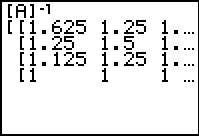
\includegraphics[width=2in]{./MatMethodsGraphics/MATRIXINVERSE01.jpg} &

\hspace{0.75in} 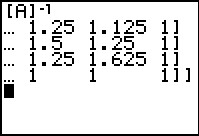
\includegraphics[width=2in]{./MatMethodsGraphics/MATRIXINVERSE02.jpg}  \\

\end{tabular}

\end{center}

from which we have  $A^{-1} = \left[ \begin{array}{rrrr} 1.625 & \hphantom{2}1.25 & 1.125 & \hphantom{2.2}1  \\ 1.25 & 1.5 & 1.25 & 1 \\ 1.125 & 1.25 & 1.625 & 1 \\ 1 & 1 & 1 & 1 \end{array} \right]$. 

To solve the four systems given to us, we find $X=A^{-1}B$ where the value of $B$ is determined by the given values of $V\!B_{\mbox{\tiny$1$}}$ and $V\!B_{\mbox{\tiny$2$}}$

\[\begin{array}{cccc}

 B = \left[ \begin{array}{r} 10 \\ 0 \\ -5 \\ 0 \end{array} \right], & 

 B = \left[ \begin{array}{r} 10 \\ 0 \\ 0 \\ 0 \end{array} \right], & 

B = \left[ \begin{array}{r} 0 \\ 0 \\ -10 \\ 0 \end{array} \right], & 

 B = \left[ \begin{array}{r} 10 \\ 0 \\ 10 \\ 0 \end{array} \right] 

\end{array} \]

\begin{itemize}

\item  For $V\!B_{\mbox{\tiny$1$}} = 10 V$ and $V\!B_{\mbox{\tiny$2$}} = 5 V$, the calculator gives $i_{\mbox{\tiny$1$}} = 10.625 \, \, mA$, $i_{\mbox{\tiny$2$}} = 6.25 \, \, mA$, $i_{\mbox{\tiny$3$}} = 3.125 \, \, mA$, and $i_{\mbox{\tiny$4$}} = 5 \, \, mA$.  We include a calculator screenshot below for this part (and this part only!) for reference.


\centerline{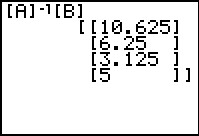
\includegraphics[width=2in]{./MatMethodsGraphics/MATRIXINVERSE03.jpg}}


\item  By keeping  $V\!B_{\mbox{\tiny$1$}} = 10 V$ and setting $V\!B_{\mbox{\tiny$2$}} = 0 V$, we are removing the effect of the second battery. We get $i_{\mbox{\tiny$1$}} = 16.25 \, \, mA$, $i_{\mbox{\tiny$2$}} = 12.5 \, \, mA$, $i_{\mbox{\tiny$3$}} = 11.25 \, \, mA$, and $i_{\mbox{\tiny$4$}} = 10 \, \, mA$.  


\item  Here, we  are zeroing out $V\!B_{\mbox{\tiny$1$}}$ and making $V\!B_{\mbox{\tiny$2$}} = 10$, essentially removing the effect of the first battery.  We find $i_{\mbox{\tiny$1$}} = -11.25 \, \, mA$, $i_{\mbox{\tiny$2$}} = -12.5 \, \, mA$, $i_{\mbox{\tiny$3$}} = -16.25 \, \, mA$, and $i_{\mbox{\tiny$4$}} = -10 \, \, mA$, where the negatives indicate that the current is flowing in the opposite direction as is indicated on the diagram. The reader is encouraged to study the symmetry here, and if need be, hold up a mirror to the diagram to literally `see' what is happening.

\item  For $V\!B_{\mbox{\tiny$1$}} = 10 V$ and $V\!B_{\mbox{\tiny$2$}} = 10 V$, we get $i_{\mbox{\tiny$1$}} = 5 \, \, mA$, $i_{\mbox{\tiny$2$}} = 0 \, \, mA$, $i_{\mbox{\tiny$3$}} = -5 \, \, mA$, and $i_{\mbox{\tiny$4$}} = 0 \, \, mA$.  The mesh currents $i_{\mbox{\tiny$2$}}$ and $i_{\mbox{\tiny$4$}}$ being zero is a consequence of both batteries `pushing' in equal but opposite directions, causing the net flow of electrons in these two regions to cancel out. \qed

\end{itemize}

\end{ex}

\subsection{Exercises}

%% SKIPPED %% \documentclass{ximera}

\begin{document}
	\author{Stitz-Zeager}
	\xmtitle{TITLE}


\label{ExercisesforMatMethods}

In Exercises \ref{findmatinversefirst} - \ref{findmatinverselast}, find the inverse of the matrix or state that the matrix is not invertible.

\begin{multicols}{2}
\begin{enumerate}

\item $A = \left[ \begin{array}{rr} 1 & 2 \\ 3 & 4 \end{array} \right]$ \label{findmatinversefirst}
\item $B = \left[ \begin{array}{rr} 12 & -7 \\ -5 & 3 \end{array} \right]$ \label{matrixB}

\setcounter{HW}{\value{enumi}}
\end{enumerate}
\end{multicols}

\begin{multicols}{2}
\begin{enumerate}
\setcounter{enumi}{\value{HW}}

\item $C = \left[ \begin{array}{rr} 6 & 15 \\ 14 & 35 \end{array} \right]$
\item $D = \left[ \begin{array}{rr} 2 & -1 \\ 16 & -9 \end{array} \right]$ \label{matrixD}

\setcounter{HW}{\value{enumi}}
\end{enumerate}
\end{multicols}

\begin{multicols}{2}
\begin{enumerate}
\setcounter{enumi}{\value{HW}}

\item $E = \left[ \begin{array}{rrr} 3 & 0 & 4 \\ 2 & -1 & 3 \\ -3 & 2 & -5 \end{array} \right]$ \label{matrixE}
\item $F = \left[ \begin{array}{rrr} 4 & \hphantom{-}6 & -3 \\ 3 & 4 & -3 \\ 1 & 2 & 6 \end{array} \right]$

\setcounter{HW}{\value{enumi}}
\end{enumerate}
\end{multicols}

\begin{multicols}{2}
\begin{enumerate}
\setcounter{enumi}{\value{HW}}

\item $G = \left[ \begin{array}{rrr} 1 & \hphantom{1}2 & 3 \\ 2 & 3 & 11 \\ 3 & 4 & 19 \end{array} \right]$
\item $H = \left[ \begin{array}{rrrr} 1 & 0 & -3 & \hphantom{-}0 \\ 2 & -2 & 8 & 7 \\ -5 & 0 & 16 & 0 \\ 1 & 0 & 4 & 1 \end{array} \right]$ \label{findmatinverselast}

\setcounter{HW}{\value{enumi}}
\end{enumerate}
\end{multicols}


In Exercises \ref{2by2inversefirst} - \ref{2by2inverselast}, use one matrix inverse to solve the following systems of linear equations.

\begin{multicols}{3}
\begin{enumerate}
\setcounter{enumi}{\value{HW}}

\item $\left\{ \begin{array}{rcr}   3x + 7y & = & 26 \\ 5x + 12y & = & 39  \end{array} \right.$ \label{2by2inversefirst}
\item $\left\{ \begin{array}{rcr}   3x + 7y & = &  0 \\ 5x + 12y & = & -1  \end{array} \right.$
\item $\left\{ \begin{array}{rcr}   3x + 7y & = & -7 \\ 5x + 12y & = &  5  \end{array} \right.$ \label{2by2inverselast}


\setcounter{HW}{\value{enumi}}
\end{enumerate}
\end{multicols}


In Exercises \ref{3by3inversefirst} - \ref{3by3inverselast}, use the inverse of $E$ from Exercise \ref{matrixE} above to solve the following systems of linear equations.

\begin{multicols}{3}
\begin{enumerate}
\setcounter{enumi}{\value{HW}}

\item $\left\{ \begin{array}{rcr}   3x + 4z & = & 1 \\ 2x - y + 3z & = & 0 \\ \!-3x + 2y - 5z & = & 0  \end{array} \right.$ \label{3by3inversefirst}
\item $\left\{ \begin{array}{rcr}   3x + 4z & = & 0 \\ 2x - y + 3z & = & 1 \\ \!-3x + 2y - 5z & = & 0  \end{array} \right.$
\item $\left\{ \begin{array}{rcr}   3x + 4z & = & 0 \\ 2x - y + 3z & = & 0 \\ \!-3x + 2y - 5z & = & 1  \end{array} \right.$ \label{3by3inverselast}

\setcounter{HW}{\value{enumi}}
\end{enumerate}
\end{multicols}

\begin{enumerate}
\setcounter{enumi}{\value{HW}}

\item  This exercise is a continuation of Example \ref{rotationmatrixex} in Section \ref{MatArithmetic} and gives another application of matrix inverses.  Recall that given the position matrix $P$ for a point in the plane, the matrix $RP$ corresponds to a point rotated $45^{\circ}$ counterclockwise from $P$ where
 
\[R = \left[ \begin{array}{rr} \frac{\sqrt{2}}{2} & -\frac{\sqrt{2}}{2} \\[3pt] \frac{\sqrt{2}}{2} & \frac{\sqrt{2}}{2} \\ \end{array} \right]\]
 
\begin{enumerate}

\item  Find $R^{-1}$.
\item  If $RP$ rotates a point counterclockwise $45^{\circ}$, what should $R^{-1}P$ do?  Check your answer by finding $R^{-1}P$ for various points on the coordinate axes and the lines $y=\pm x$.
\item  Find $R^{-1}P$ where $P$ corresponds to a generic point $P(x,y)$. Verify that this takes points on the curve $y=\frac{2}{x}$ to points on the curve $x^2-y^2=4$.

\end{enumerate}

\item \label{SasquatchDiet} A Sasquatch's diet consists of three primary foods:  Ippizuti Fish, Misty Mushrooms, and Sun Berries.  Each serving of Ippizuti Fish is 500 calories, contains 40 grams of protein, and has no Vitamin X.  Each serving of Misty Mushrooms is 50 calories, contains 1 gram of protein, and 5 milligrams of Vitamin X.  Finally, each serving of Sun Berries is 80 calories, contains no protein, but has 15 milligrams of Vitamin X.\footnote{Misty Mushrooms and Sun Berries are the only known fictional sources of Vitamin X.}

\begin{enumerate}

\item  If an adult male Sasquatch requires 3200 calories, 130 grams of protein, and 275 milligrams of Vitamin X daily, use a matrix inverse to find how many servings each of Ippizuti Fish, Misty Mushrooms, and Sun Berries he needs to eat each day.

\item  An adult female Sasquatch requires 3100 calories, 120 grams of protein, and 300 milligrams of Vitamin X daily. Use the matrix inverse you found in part (a) to find how many servings each of Ippizuti Fish, Misty Mushrooms, and Sun Berries she needs to eat each day.

\item  An adolescent Sasquatch requires 5000 calories, 400 grams of protein daily, but no Vitamin X daily.\footnote{Vitamin X is needed to sustain Sasquatch longevity only.}   Use the matrix inverse you found in part (a) to find how many servings each of Ippizuti Fish, Misty Mushrooms, and Sun Berries she needs to eat each day.

\end{enumerate}


\item Matrices can be used in cryptography.  Suppose we wish to encode the message `BIGFOOT LIVES'.  We start by assigning a number to each letter of the alphabet, say $A=1$, $B=2$ and so on.  We reserve $0$ to act as a space.  Hence, our message `BIGFOOT LIVES' corresponds to the string of numbers `2, 9, 7, 6, 15, 15, 20, 0, 12, 9, 22, 5, 19.' To encode this message, we use an invertible matrix.  Any invertible matrix will do, but for this exercise, we choose

\[ A = \left[ \begin{array}{rrr} 2 & -3 & 5 \\ 3 & 1 &-2 \\ -7 & 1 & -1 \end{array} \right] \]

Since $A$ is  $3 \times 3$ matrix, we encode our message string into a matrix $M$ with $3$ rows.  To do this, we take the first three numbers, 2 9 7, and make them our first column, the next three numbers, 6 15 15, and make them our second column, and so on.  We put $0$'s to round out the matrix.


\[ M = \left[  \begin{array}{rrrrr} 2 & 6 & 20 & 9 & 19 \\ 9 & 15 & 0 & 22 & 0 \\ 7 & 15 & 12 & 5 & 0 \end{array} \right] \]

To encode the message, we find the product $AM$

\[AM =  \left[ \begin{array}{rrr} 2 & -3 & 5 \\ 3 & 1 &-2 \\ -7 & 1 & -1 \end{array} \right]\left[  \begin{array}{rrrrr} 2 & 6 & 20 & 9 & 19 \\ 9 & 15 & 0 & 22 & 0 \\ 7 & 15 & 12 & 5 & 0 \end{array} \right] = \left[  \begin{array}{rrrrr} 12 & 42 & 100 & -23 & 38 \\ 1 & 3 & 36 & 39 & 57 \\ -12 & -42 & -152 & -46 & -133 \end{array} \right]\]

So our coded message is `12, 1, $-12$, 42, 3, $-42$, 100, 36, $-152$, $-23$, 39, $-46$, 38, 57, $-133$.'  To decode this message, we start with this string of numbers, construct a message matrix as we did earlier (we should get the matrix $AM$ again) and then multiply by $A^{-1}$.

\begin{enumerate}

\item  Find $A^{-1}$.

\item  Use $A^{-1}$ to decode the message and check this method actually works.

\item  Decode the message `14, 37, $-76$, 128, 21, $-151$, 31, 65, $-140$'

\item  Choose another invertible matrix and encode and decode your own messages.

\end{enumerate}

\item Using the matrices $A$ from Exercise \ref{findmatinversefirst}, $B$ from Exercise \ref{matrixB} and $D$ from Exercise \ref{matrixD}, show $AB = D$ and  $D^{-1} = B^{-1}A^{-1}$.  That is, show that $(AB)^{-1} = B^{-1}A^{-1}$. 

\item Let $M$ and $N$ be invertible $n \times n$ matrices.  Show that $(MN)^{-1} = N^{-1}M^{-1}$ and compare your work to Exercise \ref{fcircginverse} in Section \ref{InverseFunctions}.


\end{enumerate}

\newpage

\subsection{Answers}

\begin{multicols}{2} 
\begin{enumerate}


\item $A^{-1} = \left[ \begin{array}{rr} -2 & 1 \\[3pt] \frac{3}{2} & -\frac{1}{2} \end{array} \right]$
\item $B^{-1} = \left[ \begin{array}{rr} 3 & 7 \\ 5 & 12 \end{array} \right]$

\setcounter{HW}{\value{enumi}}
\end{enumerate}
\end{multicols}

\begin{multicols}{2} 
\begin{enumerate}
\setcounter{enumi}{\value{HW}}

\item $C \vphantom{\left[ \begin{array}{rr} \frac{9}{2} & -\frac{1}{2} \\ 8 & -1 \end{array} \right]}$ is not invertible
\item $D^{-1} = \left[ \begin{array}{rr} \frac{9}{2} & -\frac{1}{2} \\ 8 & -1 \end{array} \right]$

\setcounter{HW}{\value{enumi}}
\end{enumerate}
\end{multicols}

\begin{multicols}{2} 
\begin{enumerate}
\setcounter{enumi}{\value{HW}}

\item $E^{-1} = \left[ \begin{array}{rrr} -1 & 8 & 4 \\ 1 & -3 & -1 \\ 1 & -6 & -3 \end{array} \right] \vphantom{\left[ \begin{array}{rrr} -\frac{5}{2} & \frac{7}{2} & \frac{1}{2} \\[3pt] \frac{7}{4} & -\frac{9}{4} & -\frac{1}{4} \\[3pt] -\frac{1}{6} & \frac{1}{6} & \frac{1}{6} \end{array} \right]}$
\item $F^{-1} = \left[ \begin{array}{rrr} -\frac{5}{2} & \frac{7}{2} & \frac{1}{2} \\[3pt] \frac{7}{4} & -\frac{9}{4} & -\frac{1}{4} \\[3pt] -\frac{1}{6} & \frac{1}{6} & \frac{1}{6} \end{array} \right]$

\setcounter{HW}{\value{enumi}}
\end{enumerate}
\end{multicols}

\begin{multicols}{2} 
\begin{enumerate}
\setcounter{enumi}{\value{HW}}

\item $G \vphantom{\left[ \begin{array}{rrrr} 16 & 0 & 3 & 0 \\[3pt] -90 & -\frac{1}{2} & -\frac{35}{2} & \frac{7}{2} \\[3pt] 5 & 0 & 1 & 0 \\[3pt] -36 & 0 & -7 & \hphantom{-}1 \end{array} \right]}$ is not invertible
\item $H^{-1} = \left[ \begin{array}{rrrr} 16 & 0 & 3 & 0 \\[3pt] -90 & -\frac{1}{2} & -\frac{35}{2} & \frac{7}{2} \\[3pt] 5 & 0 & 1 & 0 \\[3pt] -36 & 0 & -7 & \hphantom{-}1 \end{array} \right]$

\setcounter{HW}{\value{enumi}}
\end{enumerate}
\end{multicols}

The coefficient matrix is $B^{-1}$ from Exercise \ref{matrixB} above so the inverse we need is $(B^{-1})^{-1} = B$. 

\begin{enumerate}
\setcounter{enumi}{\value{HW}}

\item $\left[ \begin{array}{rr} 12 & -7 \\ -5 & 3 \end{array} \right] \left[ \begin{array}{r} 26 \\ 39 \end{array} \right] = \left[ \begin{array}{r} 39 \\ -13 \end{array} \right] \;$ So $x = 39$ and $y = -13$.
\item $\left[ \begin{array}{rr} 12 & -7 \\ -5 & 3 \end{array} \right] \left[ \begin{array}{r} 0 \\ -1 \end{array} \right] = \left[ \begin{array}{r} 7 \\ -3 \end{array} \right] \;$ So $x = 7$ and $y = -3$.
\item $\left[ \begin{array}{rr} 12 & -7 \\ -5 & 3 \end{array} \right] \left[ \begin{array}{r} -7 \\ 5 \end{array} \right] = \left[ \begin{array}{r} -119 \\ 50 \end{array} \right] \;$ So $x = -119$ and $y = 50$.

\setcounter{HW}{\value{enumi}}
\end{enumerate}

The coefficient matrix is $E = \left[ \begin{array}{rrr} 3 & 0 & 4 \\ 2 & -1 & 3 \\ -3 & 2 & -5 \end{array} \right]$ from Exercise \ref{matrixE}, so $E^{-1} = \left[ \begin{array}{rrr} -1 & 8 & 4 \\ 1 & -3 & -1 \\ 1 & -6 & -3 \end{array} \right]$ 

\begin{enumerate}
\setcounter{enumi}{\value{HW}}

\item $\left[ \begin{array}{rrr} -1 & 8 & 4 \\ 1 & -3 & -1 \\ 1 & -6 & -3 \end{array} \right] \left[ \begin{array}{r} 1 \\ 0 \\ 0 \end{array} \right] = \left[ \begin{array}{r} -1 \\ 1 \\ 1 \end{array} \right] \;$ So $x = -1$, $y = 1$ and $z = 1$.
\item $\left[ \begin{array}{rrr} -1 & 8 & 4 \\ 1 & -3 & -1 \\ 1 & -6 & -3 \end{array} \right] \left[ \begin{array}{r} 0 \\ 1 \\ 0 \end{array} \right] = \left[ \begin{array}{r} 8 \\ -3 \\ -6 \end{array} \right] \;$ So $x = 8$, $y = -3$ and $z = -6$.
\item $\left[ \begin{array}{rrr} -1 & 8 & 4 \\ 1 & -3 & -1 \\ 1 & -6 & -3 \end{array} \right] \left[ \begin{array}{r} 0 \\ 0 \\ 1 \end{array} \right] = \left[ \begin{array}{r} 4 \\ -1 \\ -3 \end{array} \right] \;$ So $x = 4$, $y = -1$ and $z = -3$.

\setcounter{HW}{\value{enumi}}
\end{enumerate}

\begin{enumerate}
\setcounter{enumi}{\value{HW}}

\addtocounter{enumi}{1}

\item  \begin{enumerate} \item  The adult male Sasquatch needs:  3 servings of Ippizuti Fish, 10 servings of Misty Mushrooms, and 15 servings of Sun Berries daily.

\item  The adult female Sasquatch needs:  3 servings of Ippizuti Fish and 20 servings of Sun Berries daily.  (No Misty Mushrooms are needed!)

\item  The adolescent Sasquatch requires 10 servings of Ippizuti Fish daily.  (No Misty Mushrooms or Sun Berries are needed!)

\end{enumerate}

\item  \begin{enumerate}

\item  $A^{-1} = \left[ \begin{array}{rrr} 1 & 2 & 1 \\ 17 & 33 & 19 \\ 10 & 19 & 11 \end{array} \right] $

\item  $ \left[ \begin{array}{rrr} 1 & 2 & 1 \\ 17 & 33 & 19 \\ 10 & 19 & 11 \end{array} \right] \left[  \begin{array}{rrrrr} 12 & 42 & 100 & -23 & 38 \\ 1 & 3 & 36 & 39 & 57 \\ -12 & -42 & -152 & -46 & -133 \end{array} \right] =  \left[  \begin{array}{rrrrr} 2 & 6 & 20 & 9 & 19 \\ 9 & 15 & 0 & 22 & 0 \\ 7 & 15 & 12 & 5 & 0 \end{array} \right] \quad \checkmark$

\item  `LOGS RULE'

\end{enumerate}

\end{enumerate}

\end{document}


\closegraphsfile

\end{document}


\newpage

\section{Determinants and Cramer's Rule}

\documentclass{ximera}

\begin{document}
	\author{Stitz-Zeager}
	\xmtitle{TITLE}


\mfpicnumber{1}

\opengraphsfile{Determinants}

\setcounter{footnote}{0}

\label{Determinants}

\setlength{\extrarowheight}{0pt}

\subsection{Definition and Properties of the Determinant}

\label{determinantdefnandprops}

In this section we assign to each square matrix $A$ a real number, called the \textit{determinant} of $A$, which will eventually lead us to yet another technique for solving consistent independent systems of linear equations.  The determinant is defined recursively, that is, we define it for $1 \times 1$ matrices and give a rule by which we can reduce determinants of $n \times n$ matrices to a sum of determinants of $(n-1) \times (n-1)$ matrices.\footnote{We will talk more about the term `recursively' in Section \ref{Sequences}.}  This means we will be able to evaluate the determinant of a $2 \times 2$ matrix as a sum of the determinants of $1 \times 1$ matrices;  the determinant of a $3 \times 3$ matrix as a sum of the determinants of $2 \times 2$ matrices, and so forth.  

To explain how we will take an $n \times n$ matrix and distill an $(n-1) \times (n-1)$ matrix from it, we use introduce the following notation.

\smallskip

\colorbox{ResultColor}{\bbm
\begin{defn} \label{Aijdefn} Given an $n \times n$ matrix $A$ where $n>1$, the matrix $A_{ij}$ is the $(n-1) \times (n-1)$ matrix formed by deleting the $i$th row of $A$ and the $j$th column of $A$. 
\end{defn}
\ebm}

\smallskip

For the matrix $A$ below, we obtain $A_{\mbox{\tiny$23$}}$ by deleting the second row and third column of $A$:

\[ \begin{array}{ccc}

A = \left[ \begin{array}{rr>{\columncolor[gray]{0.7}}r} 3 &  1 & 2 \\ \rowcolor[gray]{0.7} 0 & -1 & 5 \\ 2 & 1 & 4 \\ \end{array} \right]
&
\xrightarrow{\text{Delete $R2$ and $C3$}}

&

A_{\mbox{\tiny$23$}} = \left[ \begin{array}{rr} 3 & 1 \\ 2 & 1 \\ \end{array} \right] \\

\end{array}\]

We are now in the position to define the determinant of a matrix.

\smallskip

\colorbox{ResultColor}{\bbm

\begin{defn} \label{determinantdefn} \index{matrix ! determinant ! definition of} \index{determinant of a matrix ! definition of} Given an $n \times n$ matrix $A$ the \textbf{determinant of \boldmath $A$}, denoted $\det(A)$, is defined as follows

\begin{itemize}

\item  If $n=1$, then $A = \left[ a_{\mbox{\tiny$11$}} \right]$ and $\det(A) = \det\left( \left[ a_{\mbox{\tiny$11$}} \right] \right) = a_{\mbox{\tiny$11$}}$.

\item  If $n>1$, then $A = \left[ a_{ij} \right]_{n \times n}$ and \[ \det(A) = \det\left( \left[ a_{ij} \right]_{n \times n} \right) =  a_{\mbox{\tiny$11$}} \det\left(A_{\mbox{\tiny$11$}}\right)- a_{\mbox{\tiny$12$}} \det\left(A_{\mbox{\tiny$12$}}\right) + -  \ldots  + (-1)^{1+n} a_{\mbox{\tiny$1$}n} \det\left(A_{\mbox{\tiny$1$}n}\right)\]

\end{itemize}

\end{defn}
\ebm}

\smallskip

There are two commonly used notations for the determinant of a matrix $A$: `$\det(A)$' and `$|A|$'
We have chosen to use the notation $\det(A)$ as opposed to $|A|$ because we find that the latter is often confused with absolute value, especially in the context of a $1 \times 1$ matrix.  

In the expansion $a_{\mbox{\tiny$11$}} \det\left(A_{\mbox{\tiny$11$}}\right)- a_{\mbox{\tiny$12$}} \det\left(A_{\mbox{\tiny$12$}}\right) + -  \ldots  + (-1)^{1+n} a_{\mbox{\tiny$1$}n} \det\left(A_{\mbox{\tiny$1$}n}\right)$, the notation `$+ -  \ldots  + (-1)^{1+n} a_{\mbox{\tiny$1$}n}$' means that the signs alternate and the final sign is dictated by the sign of the quantity $(-1)^{1+n}$. 

Since the entries $a_{\mbox{\tiny$11$}}$, $a_{\mbox{\tiny$12$}}$ and so forth up through $a_{\mbox{\tiny$1$}n}$ comprise the first row of $A$, we say we are finding the determinant of $A$  by `expanding along the first row'. Later in the section, we will develop a formula for $\det(A)$ which allows us to find it by expanding along any row.

\smallskip

Applying Definition \ref{determinantdefn} to the matrix $A = \left[ \begin{array}{rr} 4 & -3 \\ 2 & 1 \\ \end{array} \right]$ we get

\[ \begin{array}{rcl} 

\det(A) & = & \det \left( \left[ \begin{array}{rr} 4 & -3 \\ 2 & 1 \\ \end{array} \right] \right)\\[13pt]
& = &   4\det\left(A_{\mbox{\tiny$11$}}\right) - (-3)\det\left(A_{\mbox{\tiny$12$}}\right)\\
& = & 4 \det([1]) +3\det([2]) \\
& = & 4(1) + 3(2) \\
& = & 10 \\ \end{array}\]

For a generic $2 \times 2$ matrix $A = \left[ \begin{array}{cc} a & b \\ c & d \\ \end{array} \right]$ we get

\[ \begin{array}{rcl} 

\det(A) & = & \det \left( \left[ \begin{array}{cc}  a & b \\ c & d \\ \end{array} \right] \right)\\[13pt]
 & = &  a \det\left(A_{\mbox{\tiny$11$}}\right) - b \det\left(A_{\mbox{\tiny$12$}}\right) \\
& = &  a \det\left(\left[ d \right]\right) - b \det\left(\left[c \right]\right) \\
& = & ad-bc \end{array}\]

This formula is worth remembering

\smallskip

\colorbox{ResultColor}{\bbm
\begin{eqn} \label{2by2determinant} For a $2 \times 2$ matrix,


\[ \det \left( \left[ \begin{array}{cc}  a & b \\ c & d \\ \end{array} \right] \right) = ad-bc \]

\end{eqn}
\ebm}
\smallskip

Applying Definition \ref{determinantdefn} to the $3 \times 3$ matrix $A =  \left[ \begin{array}{rrr} 3 & 1 & \hphantom{-}2 \\ 0 & -1 & 5 \\ 2 & 1 & 4 \\ \end{array} \right]$ we obtain

\[ \begin{array}{rcl} 

\det(A) & = & \det \left( \left[ \begin{array}{rrr} 3 & 1 & \hphantom{-}2 \\ 0 & -1 & 5 \\ 2 & 1 & 4 \\ \end{array} \right] \right)\\[13pt]
        & = & 3\det\left(A_{\mbox{\tiny$11$}}\right) - 1\det\left(A_{\mbox{\tiny$12$}}\right) + 2\det\left(A_{\mbox{\tiny$13$}}\right) \\[13pt]
        & = & 3\det \left( \left[ \begin{array}{rr} -1 & 5 \\ 1 & 4 \\ \end{array} \right] \right) - \det \left( \left[ \begin{array}{rr} 0 & 5 \\ 2 & 4 \\ \end{array} \right] \right) + 2 \det \left( \left[ \begin{array}{rr} 0 & -1 \\ 2 & 1 \\ \end{array} \right] \right) \\[13pt]
        & = & 3((-1)(4) - (5)(1)) - ((0)(4)-(5)(2))+2((0)(1)-(-1)(2)) \\
        & = & 3(-9)-(-10)+2(2) \\
        & = & -13 \\ \end{array}  \]

To evaluate the determinant of a $4 \times 4$ matrix, we would have to evaluate the determinants of \textit{four} $3 \times 3$ matrices, each of which involves the finding the determinants of \textit{three} $2 \times 2$ matrices. As you can see, our method of evaluating determinants quickly gets out of hand and many of you may be reaching for the calculator.  There is some mathematical machinery which can assist us in calculating determinants and we present that here.  Before we state the theorem, we need some more terminology.

\smallskip

\colorbox{ResultColor}{\bbm

\begin{defn}  \label{minorcofactordefn} Let $A$ be an $n \times n$ matrix and $A_{ij}$ be defined as in Definition \ref{Aijdefn}.  

\begin{itemize}

\item The \index{matrix ! minor} \index{minor} \textbf{\boldmath $ij$ minor} of $A$, denoted $M_{ij}$ is defined by $M_{ij} = \det\left(A_{ij}\right)$. 

\item The \index{matrix ! cofactor}\index{cofactor}\textbf{\boldmath $ij$ cofactor} of $A$, denoted $C_{ij}$ is defined by $C_{ij} = (-1)^{i+j}M_{ij} = (-1)^{i+j}\det\left(A_{ij}\right)$. 

\end{itemize}

\end{defn}

\ebm}

\smallskip

We note that in Definition \ref{determinantdefn}, the sum 

\[a_{\mbox{\tiny$11$}} \det\left(A_{\mbox{\tiny$11$}}\right)- a_{\mbox{\tiny$12$}} \det\left(A_{\mbox{\tiny$12$}}\right) + -  \ldots  + (-1)^{1+n} a_{\mbox{\tiny$1$}n} \det\left(A_{\mbox{\tiny$1$}n}\right)\]

can be rewritten as

\[a_{\mbox{\tiny$11$}} (-1)^{1+1} \det\left(A_{\mbox{\tiny$11$}}\right) + a_{\mbox{\tiny$12$}} (-1)^{1+2} \det\left(A_{\mbox{\tiny$12$}}\right) + \ldots  + a_{\mbox{\tiny$1$}n} (-1)^{1+n} \det\left(A_{\mbox{\tiny$1$}n}\right)\]

which, in the language of cofactors is

\[a_{\mbox{\tiny$11$}} C_{\mbox{\tiny$11$}} + a_{\mbox{\tiny$12$}}C_{\mbox{\tiny$12$}} + \ldots  + a_{\mbox{\tiny$1$}n}C_{\mbox{\tiny$1$}n} \]

We are now ready to state our main theorem concerning determinants.

\smallskip

\colorbox{ResultColor}{\bbm

\begin{thm} \label{determinantprops}  \textbf{Properties of the Determinant:} Let $A = \left[a_{ij}\right]_{n \times n}$. \index{determinant of a matrix ! properties of} \index{matrix ! determinant ! properties of}

\begin{itemize}

\item  We may find the determinant by expanding along any row.  That is, for any $1 \leq k \leq n$, 

\[\det(A) = a_{k\mbox{\tiny$1$}}C_{k\mbox{\tiny$1$}} +  a_{k\mbox{\tiny$2$}}C_{k\mbox{\tiny$2$}} + \ldots + a_{kn} C_{kn}\]

\item  If $A'$ is the matrix obtained from $A$ by:

\begin{itemize}

\item interchanging any two rows, then $\det(A')=-\det(A)$.

\item  replacing a row with a nonzero multiple (say $c$) of itself, then $\det(A')=c\det(A)$

\item  replacing a row with itself plus a multiple of another row, then $\det(A')=\det(A)$

\end{itemize}

\item  If $A$ has two identical rows, or a row consisting of all $0$'s, then $\det(A) = 0$.

\item  If $A$ is upper or lower triangular,\footnote{See Exercise \ref{triangularmatrices} in \ref{MatArithmetic}.} then $\det(A)$ is the product of the entries on the main diagonal.\footnote{See page \pageref{maindiagonal} in Section \ref{MatArithmetic}.}

\item  If $B$ is an $n \times n$ matrix, then $\det(AB) = \det(A) \det(B)$.

\item  $\det\left(A^{n}\right) = \det(A)^{n}$ for all natural numbers $n$.

\item  $A$ is invertible if and only if $\det(A) \neq 0$.  In this case, $\det\left(A^{-1}\right) = \dfrac{1}{\det(A)}$.

\end{itemize}

\end{thm}

\ebm}

\smallskip

Unfortunately, while we can easily \textit{demonstrate} the results in Theorem \ref{determinantprops}, the proofs of most of these properties are beyond the scope of this text.  We could prove these properties for generic $2 \times 2$ or even $3 \times 3$ matrices by brute force computation, but this manner of proof belies the elegance and symmetry of the determinant.  We will prove what few properties we can after we have developed some more tools such as the Principle of Mathematical Induction in Section \ref{Induction}.\footnote{For a very elegant treatment, take a course in Linear Algebra.  There, you will most likely see the treatment of determinants logically reversed than what is presented here.  Specifically, the determinant is defined as a function which takes a square matrix to a real number and satisfies some of the properties in Theorem \ref{determinantprops}. From that function, a formula for the determinant is developed.}  

For the moment, let us demonstrate some of the properties listed in Theorem \ref{determinantprops} on the matrix $A$ below.  (Others will be discussed in the Exercises.)

\[A =  \left[ \begin{array}{rrr} 3 & 1 & \hphantom{-}2 \\ 0 & -1 & 5 \\ 2 & 1 & 4 \\ \end{array} \right] \]

We found $\det(A) = -13$ by expanding along the first row.  To take advantage of the $0$ in the second row, we use Theorem \ref{determinantprops} to find $\det(A) = -13$ by expanding along that row.

\[ \begin{array}{rcl} 

\det \left( \left[ \begin{array}{rrr} 3 & 1 & \hphantom{-}2 \\ 0 & -1 & 5 \\ 2 & 1 & 4 \\ \end{array} \right] \right)& = & 0C_{\mbox{\tiny$21$}} + (-1)C_{\mbox{\tiny$22$}}+5C_{\mbox{\tiny$23$}} \\

& = &  (-1) (-1)^{2+2} \det\left(A_{\mbox{\tiny$22$}}\right) + 5 (-1)^{2+3}\det\left(A_{\mbox{\tiny$23$}}\right) \\[13pt]
        
        & = & - \det \left( \left[ \begin{array}{rr} 3 & 2 \\ 2 & 4 \\ \end{array} \right] \right) -5 \det \left( \left[ \begin{array}{rr} 3 & 1 \\ 2 & 1 \\ \end{array} \right] \right) \\[13pt]
        & = & -((3)(4)-(2)(2)) - 5((3)(1)-(2)(1)) \\
        & = & -8-5 \\
        & = & -13 \, \, \checkmark \\ \end{array}  \]

In general, the sign of $(-1)^{i+j}$ in front of the minor in the expansion of the determinant follows an alternating pattern. Below is the pattern for $2 \times 2$, $3 \times 3$ and $4 \times 4$ matrices, and it extends naturally to higher dimensions.  

\[ \begin{array}{ccc}

\left[ \begin{array}{cc} + & - \\ - & + \\ \end{array} \right] 

&
\qquad 

\left[ \begin{array}{ccc} + & - & + \\ - & + & - \\ + & - & +  \end{array} \right] 


&

\qquad

\left[ \begin{array}{cccc} + & - & + & - \\ - & + & - & +\\ + & - & + & - \\ - & + & - & + \end{array} \right] 

\end{array} \]

The reader is cautioned, however, against reading too much into these sign patterns.  In the example above, we expanded the $3 \times 3$ matrix $A$ by its second row and the term which corresponds to the second entry ended up being negative even though the sign attached to the minor is $(+)$.  These signs represent only the signs of the $(-1)^{i+j}$ in the formula;  the sign of the corresponding entry as well as the minor itself determine the ultimate sign of the term in the expansion of the determinant.

\smallskip

To illustrate some of the other properties in  Theorem \ref{determinantprops}, we use row operations to transform our $3 \times 3$ matrix $A$ into an upper triangular matrix, keeping track of the row operations, and labeling each successive matrix.  In what follows we follow the Gauss Jordan algorithm without worrying about getting leading $1$'s.


\[ \begin{array}{ccccc}

\left[ \begin{array}{rrr} 
3 &  1 & \hphantom{-}2 \\ 
0 & -1 & 5 \\ 
2 & 1 & 4 \\ 
\end{array} \right]

&
\xrightarrow[\text{with $-\frac{2}{3}R1+R3$}]{\text{Replace $R3$}}
&

\left[ \begin{array}{rrr} 
3 &  1 & \hphantom{-}2 \\ 
0 & -1 & 5 \\
0 & \frac{1}{3} & \frac{8}{3} \\ 
\end{array} \right]
&
\xrightarrow[\text{$\frac{1}{3}R2+R3$}]{\text{Replace $R3$ with}}
&

\left[ \begin{array}{rrr} 
3 &  1 & 2 \\ 
0 & -1 & 5 \\
0 & 0 & \frac{13}{3} \\ 
\end{array} \right] \\

A & & B & & C \\

\end{array}\]

Theorem \ref{determinantprops} guarantees us that $\det(A) = \det(B) = \det(C)$ since we are replacing a row with itself plus a multiple of another row moving from one matrix to the next.  Furthermore, since $C$ is upper triangular, $\det(C)$ is the product of the entries on the main diagonal, in this case  $\det(C) = (3)(-1)\left(\frac{13}{3}\right) = -13$.  This demonstrates the utility of using row operations to assist in calculating determinants.  

This also sheds some light on the connection between a determinant and invertibility.  Recall from Section \ref{MatMethods} that in order to find $A^{-1}$, we attempt to transform $A$ to $I_{n}$ using row operations

\[ \begin{array}{ccc}

\left[ \begin{array}{c|c} A & I_{n} \\ \end{array} \right]

&
\xrightarrow{\text{Gauss Jordan Elimination}}

&

\left[ \begin{array}{c|c} I_{n} & A^{-1} \\ \end{array} \right] 

\end{array}\]

As we apply our allowable row operations on $A$ to put it into reduced row echelon form, the determinant of the intermediate matrices can vary from the determinant of $A$ by at most a \textit{nonzero} multiple.  This means that if $\det(A) \neq 0$, then the determinant of $A$'s reduced row echelon form must also be nonzero.   Per  Definition \ref{rowechelonform}, this  means that all the main diagonal entries on $A$'s reduced row echelon form must be $1$.  Hence,  $A$'s reduced row echelon form is $I_{n}$ so  $A$ is invertible. 

Conversely, if $A$ is invertible, then $A$ can be transformed into $I_{n}$ using row operations.  Since $\det\left(I_{n}\right) = 1 \neq 0$, our same logic implies $\det(A) \neq 0$. Basically, we have established that the determinant \textit{determines} whether or not the matrix $A$ is invertible.\footnote{In Section \ref{CramersRuleMatrixAdjoints}, we learn determinants (specifically cofactors) are deeply connected with the inverse of a matrix.}  

\smallskip

It is worth noting that when we first introduced the notion of a matrix inverse, it was in the context of solving a linear matrix equation.  In effect, we were trying to `divide' both sides of the matrix equation $AX = B$ by the matrix $A$.  Just like we cannot divide a real number by $0$, Theorem \ref{determinantprops} tells us we cannot `divide' by a matrix whose \textit{determinant} is $0$.  We also know that if the coefficient matrix of a system of linear equations is invertible, then system is consistent and independent.  It follows, then, that if the determinant of said coefficient is not zero, the system is consistent and independent.  

\newpage

\subsection{Cramer's Rule and Matrix Adjoints}
\label{CramersRuleMatrixAdjoints}

In this section, we introduce a theorem which enables us to solve a system of linear equations by means of determinants only.  As usual, the theorem is stated in full generality, using numbered unknowns $x_{\mbox{\tiny$1$}}$, $x_{\mbox{\tiny$2$}}$, etc., instead of the more familiar letters $x$, $y$, $z$, etc.   As with many results in this chapter, the proof of the general case is best left to a course in Linear Algebra.

\smallskip

\colorbox{ResultColor}{\bbm

\begin{thm} \label{CramersRule} \index{Cramer's Rule} \textbf{Cramer's Rule:} Suppose  $AX = B$ is the matrix form of a system of $n$ linear equations in $n$ unknowns where $A$ is the coefficient matrix, $X$ is the unknowns matrix, and $B$ is the constant matrix. 

If $\det(A) \neq 0$, then the corresponding system is consistent and independent and the solution for unknowns $x_{\mbox{\tiny$1$}}$, $x_{\mbox{\tiny$2$}}$, \ldots $x_{n}$ is given by:

\[ x_{j} = \dfrac{\det\left(A_{j}\right)}{\det(A)},\]

where $A_{j}$ is the matrix $A$ whose $j$th column has been replaced by the constants in $B$.

\end{thm}

\ebm}

\smallskip

In words, Cramer's Rule tells us we can solve for each unknown, one at a time, by finding the ratio of the determinant of $A_{j}$ to that of the determinant of the coefficient matrix.  The matrix $A_{j}$ is found by replacing the column in the coefficient matrix which holds the coefficients of $x_{j}$ with the constants of the system.  The following example fleshes out this method.

\smallskip

\begin{ex}  Use Cramer's Rule to solve for the indicated unknowns.

\begin{enumerate}

\item  Solve $\left\{ \begin{array}{rcr} 2x_{\mbox{\tiny$1$}} - 3x_{\mbox{\tiny$2$}} & = & 4 \\ 5x_{\mbox{\tiny$1$}} + x_{\mbox{\tiny$2$}} & = & -2   \end{array} \right.$ for $x_{\mbox{\tiny$1$}}$ and $x_{\mbox{\tiny$2$}}$

\item  Solve $\left\{ \begin{array}{rcr} 2x - 3y + z & = & -1 \\ x-y+z & = & 1 \\ 3x-4z & = & 0   \end{array} \right.$ for $z$.

\end{enumerate}

{\bf Solution.}  

\begin{enumerate}

\item  Writing this system in matrix form, we find 

\[ \begin{array}{ccc}

A = \left[ \begin{array}{rr} 2 & -3 \\ 5 & 1 \\ \end{array} \right] 
&
\qquad X = \left[ \begin{array}{r} x_{\mbox{\tiny$1$}} \\ x_{\mbox{\tiny$2$}} \\ \end{array} \right] 
& 
\qquad B = \left[ \begin{array}{r} 4 \\ -2 \\ \end{array} \right] \\

\end{array} \]

To find the matrix $A_{\mbox{\tiny$1$}}$, we remove the column of the coefficient matrix $A$ which holds the coefficients of $x_{\mbox{\tiny$1$}}$ and replace it with the corresponding entries in $B$.  Likewise, we replace the column of $A$ which corresponds to the coefficients of $x_{\mbox{\tiny$2$}}$ with the constants to form the matrix $A_{\mbox{\tiny$2$}}$.  This yields 

\[ \begin{array}{cc}

A_{\mbox{\tiny$1$}} = \left[ \begin{array}{rr} 4 & -3 \\ -2 & 1 \\ \end{array} \right] 

&

\qquad A_{\mbox{\tiny$2$}} = \left[ \begin{array}{rr} 2 & 4 \\ 5 & -2 \\ \end{array} \right] \\

\end{array} \]

Computing determinants, we get $\det(A) = 17$, $\det\left(A_{\mbox{\tiny$1$}}\right) = -2$ and  $\det\left(A_{\mbox{\tiny$2$}}\right) = -24$, so that

\[ \begin{array}{cc}

x_{\mbox{\tiny$1$}} = \dfrac{\det\left(A_{\mbox{\tiny$1$}}\right)}{\det(A)} = -\dfrac{2}{17} 
& 
\qquad x_{\mbox{\tiny$2$}} = \dfrac{\det\left(A_{\mbox{\tiny$2$}}\right)}{\det(A)} = -\dfrac{24}{17} \\

\end{array} \]

The reader can check that the solution to the system is $\left(-\frac{2}{17}, -\frac{24}{17}\right)$.

\item To use Cramer's Rule to find $z$, we identify $x_{\mbox{\tiny$3$}}$ as $z$.  We have 

\[ \begin{array}{cccc}

A = \left[ \begin{array}{rrr} 2 & -3 & 1 \\ 1 & -1 & 1 \\ 3 & 0 & -4  \end{array} \right] 
&
 X = \left[ \begin{array}{r} x \\ y \\ z \end{array} \right] 
& 
B = \left[ \begin{array}{r} -1 \\ 1 \\ 0 \end{array} \right] 

&

A_{\mbox{\tiny$3$}} = A_{z} =  \left[ \begin{array}{rrr} 2 & -3 & -1 \\ 1 & -1 & 1 \\ 3 & 0 & 0 \end{array} \right] \\

\end{array} \]

Expanding both $\det(A)$ and $\det\left(A_{z}\right)$ along the third rows (to take advantage of the $0$'s) gives

\[ z = \dfrac{\det\left(A_{z}\right)}{\det(A)} = \dfrac{-12}{-10} = \dfrac{6}{5} \]

The reader is encouraged to solve this system for $x$ and $y$ similarly and check the answer.  \qed

\end{enumerate}

\end{ex}

It is worth noting that finding determinants is very `computationally expensive' meaning they take quite a bit of time and effort to compute for humans and machines alike.  For that reason, determinants, and, in particular, Cramer's Rule are used mostly in theoretical contexts as convenient ways to describe and discuss solutions to systems of linear equations.\footnote{A classic case of this is the \href{https://en.wikipedia.org/wiki/Wronskian}{\underline{Wronskian}} from Differential Equations.}

\smallskip

Our last application of determinants is to develop an alternative method for finding the inverse of a matrix. As with the discussion in Section \ref{MatMethods} when we developed the first algorithm to find matrix inverses, we ask that you indulge us as we proceed to work to describe a \textit{general} method here via \textit{example}. 

Let us consider the $3 \times 3$ matrix $A$ which we so extensively studied in Section \ref{determinantdefnandprops}

\[A = \left[ \begin{array}{rrr} 3 & 1 & \hphantom{-}2 \\ 0 & -1 & 5 \\ 2 & 1 & 4 \\ \end{array} \right]\]

We found through a variety of methods that $\det(A) = -13$.  To our surprise and delight, its inverse below has a remarkable number of $13$'s in the denominators of its entries. This is no coincidence.

\[ A^{-1} = \left[ \begin{array}{rrr} \frac{9}{13} & \frac{2}{13} & -\frac{7}{13} \\[3pt] -\frac{10}{13} & -\frac{8}{13} & \frac{15}{13} \\[3pt] -\frac{2}{13} & \frac{1}{13} & \frac{3}{13} \\ \end{array} \right]\]

Recall that to find $A^{-1}$,  we are essentially solving the matrix equation $AX = I_{\mbox{\tiny$3$}}$, where $X = \left[ x_{ij} \right]_{3 \times 3}$ is a $3 \times 3$ matrix.  Because of how matrix multiplication is defined, the first column of $I_{\mbox{\tiny$3$}}$ is the product of $A$ with the first column of $X$, the second column of $I_{\mbox{\tiny$3$}}$ is the product of $A$ with the second column of $X$ and the third column of $I_{\mbox{\tiny$3$}}$ is the product of $A$ with the third column of $X$.  In other words, we are solving three equations\footnote{The reader is encouraged to stop and think this through.}

\[\begin{array}{ccc}

A\left[ \begin{array}{r} x_{\mbox{\tiny$11$}} \\ x_{\mbox{\tiny$21$}} \\ x_{\mbox{\tiny$31$}} \end{array} \right] = \left[ \begin{array}{r} 1 \\ 0 \\ 0 \end{array} \right]

&
\qquad
A\left[ \begin{array}{r} x_{\mbox{\tiny$12$}} \\ x_{\mbox{\tiny$22$}} \\ x_{\mbox{\tiny$32$}} \end{array} \right] = \left[ \begin{array}{r} 0 \\ 1 \\ 0 \end{array} \right] 

& 

\qquad

A\left[ \begin{array}{r} x_{\mbox{\tiny$13$}} \\ x_{\mbox{\tiny$23$}} \\ x_{\mbox{\tiny$33$}} \end{array} \right] = \left[ \begin{array}{r} 0 \\ 0 \\ 1 \end{array} \right] \\

\end{array}\]

We can solve each of these systems using Cramer's Rule.  Focusing on the first system, we have 

\[ \begin{array}{ccc}

A_{\mbox{\tiny$1$}} = \left[ \begin{array}{rrr} 1 & 1 & \hphantom{-}2 \\ 0 & -1 & 5 \\ 0 & 1 & 4 \\ \end{array} \right]

&

A_{\mbox{\tiny$2$}} = \left[ \begin{array}{rrr} 3 &  1 & 2 \\ 0 & 0 & 5 \\ 2 & 0 & 4 \\ \end{array} \right]

&

A_{\mbox{\tiny$3$}} = \left[ \begin{array}{rrr} 3 &  1 & \hphantom{-}1 \\ 0 & -1 & 0 \\ 2 & 1 & 0 \\ \end{array} \right]

\end{array} \]

If we expand $\det\left(A_{\mbox{\tiny$1$}}\right)$ along the first row, we get

\[ \begin{array}{rcl}

 \det\left(A_{\mbox{\tiny$1$}}\right) & = &  \det\left( \left[ \begin{array}{rr} -1 & 5 \\ 1 & 4 \\ \end{array} \right] \right) - \det\left( \left[ \begin{array}{rr} 0 & 5 \\ 0 & 4 \\ \end{array} \right] \right) + 2 \det\left( \left[ \begin{array}{rr} 0 & -1 \\ 0 & 1 \\ \end{array} \right] \right) \\ [13pt]
                        
                      & = & \det\left( \left[ \begin{array}{rr} -1 & 5 \\ 1 & 4 \\ \end{array} \right] \right)
                        
\end{array} \]

Amazingly, this is none other than the  $C_{\mbox{\tiny$11$}}$ cofactor of $A$.  The reader is invited to check this, as well as the claims that  $\det\left(A_{\mbox{\tiny$2$}}\right) = C_{\mbox{\tiny$12$}}$ and $\det\left(A_{\mbox{\tiny$3$}}\right) = C_{\mbox{\tiny$13$}}$.\footnote{In a solid Linear Algebra course you will learn that the properties in Theorem \ref{determinantprops} hold equally well if the word `row' is replaced by the word `column'.  We're not going to get into column operations in this text, but they do make some of what we're trying to say easier to follow.} (To see this, though it seems unnatural to do so, expand along the first row.) Cramer's Rule tells us

\[\begin{array}{ccc}

x_{\mbox{\tiny$11$}} = \dfrac{\det\left(A_{\mbox{\tiny$1$}}\right)}{\det(A)} = \dfrac{C_{\mbox{\tiny$11$}}}{\det(A)}, 
&
x_{\mbox{\tiny$21$}} = \dfrac{\det\left(A_{\mbox{\tiny$2$}}\right)}{\det(A)}  = \dfrac{C_{\mbox{\tiny$12$}}}{\det(A)}, 
&
 x_{\mbox{\tiny$31$}} = \dfrac{\det\left(A_{\mbox{\tiny$3$}}\right)}{\det(A)} = \dfrac{C_{\mbox{\tiny$13$}}}{\det(A)}


\end{array} \]

So the first column of the inverse matrix $X$ is:

\[  \left[ \begin{array}{r} x_{\mbox{\tiny$11$}} \\ x_{\mbox{\tiny$21$}} \\ x_{\mbox{\tiny$31$}} \end{array} \right] = \left[ \begin{array}{r} \dfrac{C_{\mbox{\tiny$11$}}}{\det(A)} \\ [13pt]  \dfrac{C_{\mbox{\tiny$12$}}}{\det(A)} \\  [13pt] \dfrac{C_{\mbox{\tiny$13$}}}{\det(A)} \end{array} \right] = \dfrac{1}{\det(A)} \left[ \begin{array}{r} C_{\mbox{\tiny$11$}} \\ C_{\mbox{\tiny$12$}} \\ C_{\mbox{\tiny$13$}} \end{array} \right]  \]

Notice the reversal of the subscripts going from the unknown to the corresponding cofactor of $A$. This trend continues and we get
\[ \begin{array}{cc}

\left[ \begin{array}{r} x_{\mbox{\tiny$12$}} \\ x_{\mbox{\tiny$22$}} \\ x_{\mbox{\tiny$32$}} \end{array} \right] =  \dfrac{1}{\det(A)} \left[ \begin{array}{r} C_{\mbox{\tiny$21$}} \\ C_{\mbox{\tiny$22$}} \\ C_{\mbox{\tiny$23$}} \end{array} \right]

&
\qquad

\left[ \begin{array}{r} x_{\mbox{\tiny$13$}} \\ x_{\mbox{\tiny$23$}} \\ x_{\mbox{\tiny$33$}} \end{array} \right] =  \dfrac{1}{\det(A)} \left[ \begin{array}{r} C_{\mbox{\tiny$31$}} \\ C_{\mbox{\tiny$32$}} \\ C_{\mbox{\tiny$33$}} \end{array} \right]

\end{array}\]

Putting all of these together, we have obtained a new and surprising formula for $A^{-1}$, namely

\[ A^{-1} = \dfrac{1}{\det(A)} \left[ \begin{array}{ccc} C_{\mbox{\tiny$11$}} & C_{\mbox{\tiny$21$}} & C_{\mbox{\tiny$31$}} \\ C_{\mbox{\tiny$12$}} & C_{\mbox{\tiny$22$}} & C_{\mbox{\tiny$32$}} \\ C_{\mbox{\tiny$13$}} & C_{\mbox{\tiny$23$}} & C_{\mbox{\tiny$33$}} \\ \end{array} \right] \]

To see that this does indeed yield $A^{-1}$, we find all of the cofactors of $A$

\[\begin{array}{rcrrcrrcr}

C_{\mbox{\tiny$11$}} & = & -9, & C_{\mbox{\tiny$21$}} & = & -2, & C_{\mbox{\tiny$31$}} & = & 7\\

C_{\mbox{\tiny$12$}} & = & 10, & C_{\mbox{\tiny$22$}} & = & 8, & C_{\mbox{\tiny$32$}} & = & -15 \\

C_{\mbox{\tiny$13$}} & = &  2,  & C_{\mbox{\tiny$23$}} & = & -1,  & C_{\mbox{\tiny$33$}} & = & -3 \\

\end{array} \]

And, as promised,

\[ A^{-1} = \dfrac{1}{\det(A)} \left[ \begin{array}{ccc} C_{\mbox{\tiny$11$}} & C_{\mbox{\tiny$21$}} & C_{\mbox{\tiny$31$}} \\ C_{\mbox{\tiny$12$}} & C_{\mbox{\tiny$22$}} & C_{\mbox{\tiny$32$}} \\ C_{\mbox{\tiny$13$}} & C_{\mbox{\tiny$23$}} & C_{\mbox{\tiny$33$}} \\ \end{array} \right] = -\dfrac{1}{13} \left[ \begin{array}{rrr} -9 & -2 & 7\\ 10 & 8 & -15 \\ 2  &  -1 &  -3 \\ \end{array} \right]  =  \left[ \begin{array}{rrr} \frac{9}{13} & \frac{2}{13} & -\frac{7}{13} \\[3pt] -\frac{10}{13} & -\frac{8}{13} & \frac{15}{13} \\[3pt] -\frac{2}{13} & \frac{1}{13} & \frac{3}{13} \\ \end{array} \right] \]

To generalize this to invertible $n \times n$ matrices, we need another definition and a theorem.  Our definition gives a special name to the cofactor matrix, and the theorem gives us a recipe for the matrix inverse.

\smallskip

\colorbox{ResultColor}{\bbm

\begin{defn}  \label{matrixadjoint} Let $A$ be an $n \times n$ matrix, and $C_{ij}$ denote the $ij$ cofactor of $A$.  

The \index{matrix ! adjoint}\index{adjoint of a matrix}\textbf{adjoint} of $A$, denoted $\text{adj}(A)$ is the matrix whose $ij$-entry is the $ji$ cofactor of $A$, $C_{ji}$.  That is

\[ \text{adj}(A) = \left[
\begin{array}{cccc} 
C_{\mbox{\tiny$11$}} & C_{\mbox{\tiny$21$}} & \ldots & C_{n\mbox{\tiny$1$}} \\  
C_{\mbox{\tiny$12$}} & C_{\mbox{\tiny$22$}} & \ldots & C_{n\mbox{\tiny$2$}} \\
   \vdots  & \vdots & & \vdots \\
C_{\mbox{\tiny$1$}n} & C_{\mbox{\tiny$2$}n} & \ldots & C_{nn} \\  \end{array} \right] \]


\end{defn}

\ebm}

\smallskip

This new notation greatly shortens the statement of the formula for the inverse of a matrix.

\smallskip

\colorbox{ResultColor}{\bbm

\begin{thm}  \label{adjointinverse} Let $A$ be an invertible $n \times n$ matrix.  Then

\[ A^{-1} = \dfrac{1}{\det(A)} \text{adj}(A) \]

\end{thm}

\ebm}

\smallskip

For $2 \times 2$ matrices, Theorem \ref{adjointinverse} reduces to a fairly simple formula.

\smallskip

\colorbox{ResultColor}{\bbm

\begin{eqn}   \label{2by2inverse}  For an invertible $2 \times 2$ matrix,

\[ \left[ \begin{array}{rr}  a & b \\ c & d \\ \end{array} \right]^{-1} = \dfrac{1}{ad-bc} \left[ \begin{array}{rr}  d & -b \\ -c & a \\ \end{array} \right] \]



\end{eqn}
\ebm}
\smallskip

The proof of Theorem \ref{adjointinverse} is, like so many of the results in this section, best left to a course in Linear Algebra.  In such a course, not only do you gain some more sophisticated proof techniques, you also gain a larger perspective.  Within the scope of this text, we will prove a few results involving determinants in Section \ref{Induction} using the Principle of Mathematical Induction.  Until then, make sure you have a handle on the \textit{mechanics} of matrices and the theory will come eventually.

\newpage

\subsection{Exercises}

\documentclass{ximera}

\begin{document}
	\author{Stitz-Zeager}
	\xmtitle{TITLE}
\mfpicnumber{1} \opengraphsfile{ExercisesforDeterminants} % mfpic settings added 


\label{ExercisesforDeterminants}

Exercise ideas: revisit fitting curves to three points - function condition means det not zero (?)

Determinant formula for line

Geometry of determinant  - wait to vectors (?)

Follow up in inverse determinant section:  What about $ax^m + bx^n + cx^p$ for these three points?

In Exercises \ref{finddetfirst} - \ref{finddetlast},  compute the determinant of the given matrix.  (Some of these matrices appeared in Exercises \ref{findmatinversefirst} - \ref{findmatinverselast} in Section \ref{MatMethods}.)

\begin{multicols}{2}
\begin{enumerate}

\item $B = \left[ \begin{array}{rr} 12 & -7 \\ -5 & 3 \end{array} \right]$ \label{finddetfirst}
\item $C = \left[ \begin{array}{rr} 6 & 15 \\ 14 & 35 \end{array} \right]$ \label{matrixC}

\setcounter{HW}{\value{enumi}}
\end{enumerate}
\end{multicols}

\begin{multicols}{2}
\begin{enumerate}
\setcounter{enumi}{\value{HW}}

\item $Q = \left[ \begin{array}{rr} x & x^{2} \\ 1 & 2x \end{array} \right] \vphantom{ \left[ \begin{array}{rr} \dfrac{1}{x^{3}} & \dfrac{\ln(x)}{x^{3}} \\[10pt] -\dfrac{3}{x^{4}} & \dfrac{1 - 3\ln(x)}{x^{4}} \end{array} \right]}$
\item $L = \left[ \begin{array}{rr} \dfrac{1}{x^{3}} & \dfrac{\ln(x)}{x^{3}} \\[10pt] -\dfrac{3}{x^{4}} & \dfrac{1 - 3\ln(x)}{x^{4}} \end{array} \right]$


\setcounter{HW}{\value{enumi}}
\end{enumerate}
\end{multicols}

\begin{multicols}{2}
\begin{enumerate}
\setcounter{enumi}{\value{HW}}

\item $F = \left[ \begin{array}{rrr} 4 & \hphantom{-}6 & -3 \\ 3 & 4 & -3 \\ 1 & 2 & 6 \end{array} \right]$
\item $G = \left[ \begin{array}{rrr} 1 & \hphantom{1}2 & 3 \\ 2 & 3 & 11 \\ 3 & 4 & 19 \end{array} \right]$ \label{matrixG}

\setcounter{HW}{\value{enumi}}
\end{enumerate}
\end{multicols}

\begin{multicols}{2}
\begin{enumerate}
\setcounter{enumi}{\value{HW}}

\item $V = \left[ \begin{array}{rrr} i & j & k \\ -1 & 0 & 5 \\ 9 & -4 & -2 \end{array} \right] \vphantom{\left[ \begin{array}{rrrr} 1 & 0 & -3 & 0 \\ 2 & -2 & 8 & 7 \\ -5 & 0 & 16 & 0 \\ 1 & 0 & 4 & 1 \end{array} \right]}$
\item $H = \left[ \begin{array}{rrrr} 1 & 0 & -3 & 0 \\ 2 & -2 & 8 & 7 \\ -5 & 0 & 16 & 0 \\ 1 & 0 & 4 & 1 \end{array} \right]$ \label{finddetlast}


\setcounter{HW}{\value{enumi}}
\end{enumerate}
\end{multicols}


In Exercises \ref{solvecramerfirst} - \ref{solvecramerlast},   use Cramer's Rule to solve the system of linear equations.

\begin{multicols}{2}
\begin{enumerate}
\setcounter{enumi}{\value{HW}}

\item $\left\{ \begin{array}{rcr}   3x + 7y & = & 26 \\ 5x + 12y & = & 39  \end{array} \right.$ \label{solvecramerfirst}

\item $\left\{ \begin{array}{rcr}   2x-4y & = & 5 \\ 10x + 13y & = & -6  \end{array} \right.$

\setcounter{HW}{\value{enumi}}
\end{enumerate}
\end{multicols}

\begin{multicols}{2}
\begin{enumerate}
\setcounter{enumi}{\value{HW}}

\item $\left\{ \begin{array}{rcr}   x + y & = & 8000 \\ 0.03x + 0.05y & = & 250  \end{array} \right.$

\item $\left\{ \begin{array}{rcr}   \frac{1}{2}x  - \frac{1}{5}y & = & 1 \\ 6x +7y & = & 3  \end{array} \right.$



\setcounter{HW}{\value{enumi}}
\end{enumerate}
\end{multicols}

\begin{multicols}{2}
\begin{enumerate}
\setcounter{enumi}{\value{HW}}

\item $\left\{ \begin{array}{rcr} x + y + z & = & 3 \\ 2x - y + z & = & 0 \\ -3x + 5y + 7z & = & 7  \end{array} \right.$

\item $\left\{ \begin{array}{rcr} 3x + y - 2z & = & 10 \\ 4x - y + z & = & 5 \\ x -3y - 4z & = & -1  \end{array} \right.$ \label{solvecramerlast}

\setcounter{HW}{\value{enumi}}
\end{enumerate}
\end{multicols}

In Exercises \ref{cramersinglefirst} - \ref{cramersinglelast},  use Cramer's Rule to solve for $x_{\mbox{\tiny$4$}}$.


\begin{multicols}{2}
\begin{enumerate}
\setcounter{enumi}{\value{HW}}

\item $\left\{ \begin{array}{rcr} x_{\mbox{\tiny$1$}} - x_{\mbox{\tiny$3$}} & = & -2 \\ 
2x_{\mbox{\tiny$2$}} - x_{\mbox{\tiny$4$}} & = & 0  \\  
x_{\mbox{\tiny$1$}} -  2x_{\mbox{\tiny$2$}} + x_{\mbox{\tiny$3$}} & = & 0 \\
-x_{\mbox{\tiny$3$}} + x_{\mbox{\tiny$4$}} & = & 1  \end{array} \right.$  \label{cramersinglefirst}

\item $\left\{ \begin{array}{rcr} 4x_{\mbox{\tiny$1$}} + x_{\mbox{\tiny$2$}} & = & 4 \\ 
x_{\mbox{\tiny$2$}} - 3x_{\mbox{\tiny$3$}} & = & 1  \\  
10x_{\mbox{\tiny$1$}} +x_{\mbox{\tiny$3$}} + x_{\mbox{\tiny$4$}} & = & 0 \\
-x_{\mbox{\tiny$2$}} + x_{\mbox{\tiny$3$}} & = & -3  \end{array} \right.$  \label{cramersinglelast}

\setcounter{HW}{\value{enumi}}
\end{enumerate}
\end{multicols}

\pagebreak

In Exercises \ref{invadjfirst} - \ref{invadjlast}, find the inverse of the given matrix using their determinants and adjoints.

\begin{multicols}{2}
\begin{enumerate}
\setcounter{enumi}{\value{HW}}

\item $B = \left[ \begin{array}{rr} 12 & -7 \\ -5 & 3 \end{array} \right] \vphantom{\left[ \begin{array}{rrr} 4 & \hphantom{-}6 & -3 \\ 3 & 4 & -3 \\ 1 & 2 & 6 \end{array} \right]}$ \label{invadjfirst}
\item $F = \left[ \begin{array}{rrr} 4 & \hphantom{-}6 & -3 \\ 3 & 4 & -3 \\ 1 & 2 & 6 \end{array} \right]$ \label{invadjlast}

\setcounter{HW}{\value{enumi}}
\end{enumerate}
\end{multicols}


\begin{enumerate}
\setcounter{enumi}{\value{HW}}


\item  Carl's Sasquatch Attack! Game Card Collection is a mixture of common and rare cards.  Each common card is worth $\$0.25$ while each rare card is worth $\$0.75$. If his entire 117 card collection is worth $\$48.75$, how many of each kind of card does he own?

\item  How much of a 5 gallon $40\%$ salt solution should be replaced with pure water to obtain 5 gallons of a $15 \%$ solution?

\item  How much of a 10 liter $30\%$ acid solution must be replaced with pure acid to obtain 10 liters of a $50\%$ solution?

\item  Daniel's Exotic Animal Rescue houses snakes, tarantulas and scorpions.  When asked how many animals of each kind he boards, Daniel answered:  `We board 49 total animals, and I am responsible for each of their 272 legs and 28 tails.'  How many of each animal does the Rescue board?  (Recall:  tarantulas have 8 legs and no tails,  scorpions have 8 legs and one tail, and snakes have no legs and one tail.)

\item  This exercise is a continuation of Exercise \ref{SasquatchDiet} in Section \ref{MatMethods}.  Just because a system is consistent independent doesn't mean it will admit a solution that makes sense in an applied setting. Using the nutrient values given for Ippizuti Fish, Misty Mushrooms, and Sun Berries, use Cramer's Rule to determine the number of servings of Ippizuti Fish needed to meet the needs of a daily diet which requires 2500 calories, 1000 grams of protein, and 400 milligrams of Vitamin X. Now use Cramer's Rule to find the number of servings of Misty Mushrooms required. Does a solution to this diet problem exist?    


\item Let $R = \left[ \begin{array}{rr} -7 & 3 \\ 11 & \hphantom{-} 2 \end{array} \right], \;\;\; S = \left[ \begin{array}{rr} 1 & -5 \\ 6 & 9 \end{array} \right] \;\;\; T = \left[ \begin{array}{rr} 11 & \hphantom{-} 2 \\ -7 & 3  \end{array} \right], \mbox{ and } U = \left[ \begin{array}{rr} -3 & 15 \\ 6 & 9 \end{array} \right]$

\begin{enumerate}

\item Show that $\det(RS) = \det(R)\det(S)$
\item Show that $\det(T) = -\det(R)$
\item Show that $\det(U) = -3\det(S)$

\end{enumerate}

\item For $M$,  $N$, and $P$ below, show that $\det(M) = 0$, $\det(N) = 0$ and $\det(P) = 0$. \[M = \left[ \begin{array}{rrr} 1 & 2 & 3 \\ 0 & 0 & 0 \\ 7 & 8 & 9 \end{array} \right], \quad N = \left[ \begin{array}{rrr} 1 & 2 & 3 \\ 1 & 2 & 3 \\ 4 & 5 & 6 \end{array} \right] , \quad  P =  \left[ \begin{array}{rrr} 1 & 2 & 3 \\ -2 & -4 & -6 \\ 7 & 8 & 9 \end{array} \right]  \]

\item  This exercise is a follow-up to Exercise \ref{threepointsmatrixfunctionfitex} in Section \ref{AugMatrices}.   Suppose you wish to determine coefficients $a$, $b$, and $c$ so the the graph of $f(x) = ax^{m} + bx^{n} + cx^{p}$ contains the points  $(-2,1)$, $(1,4)$, $(3,-2)$.  With help from your classmates, discuss if there a unique solution for every selection of $m$, $n$, and $p$?  If not, under what conditions is there a unique solution?

\item Let $A$ be an arbitrary invertible $3 \times 3$ matrix.  

\begin{enumerate}

\item Show that $\det(I_{\mbox{\tiny$3$}}) = 1$. (See footnote\footnote{If you think about it for just a moment, you'll see that $\det(I_{n}) = 1$ for any natural number $n$.  The formal proof of this fact requires the Principle of Mathematical Induction (Section \ref{Induction}) so we'll stick with $n = 3$ for the time being.} below.)

\item Using the facts that $AA^{-1} = I_{3}$ and $\det(AA^{-1}) = \det(A)\det(A^{-1})$, show that \[\det(A^{-1}) = \dfrac{1}{\det(A)}\]

\end{enumerate}

\setcounter{HW}{\value{enumi}}
\end{enumerate}

The purpose of Exercises \ref{eigenfirst} - \ref{eigenlast} is to introduce you to the eigenvalues and eigenvectors of a matrix.\footnote{This material is usually given its own chapter in a Linear Algebra book so clearly we're not able to tell you everything you need to know about eigenvalues and eigenvectors.  They are a nice application of determinants, though, so we're going to give you enough background so that you can start playing around with them.}  We begin with an example using a $2 \times 2$ matrix and then guide you through some exercises using a $3 \times 3$ matrix.  Consider the matrix \[C = \left[ \begin{array}{rr} 6 & 15 \\ 14 & 35 \end{array} \right]\] from Exercise \ref{matrixC}.  We know that $\det(C) = 0$ which means that $CX = 0_{\mbox{\tiny$2$} \times \mbox{\tiny$2$}}$ does not have a unique solution.  So there is a nonzero matrix $Y$ with $CY = 0_{\mbox{\tiny$2$} \times \mbox{\tiny$2$}}$.  In fact, every matrix of the form \[Y = \left[ \begin{array}{r} -\frac{5}{2}t \\[3pt] t  \end{array} \right]\] is a solution to $CX = 0_{\mbox{\tiny$2$} \times \mbox{\tiny$2$}}$, so there are infinitely many matrices such that $CX = 0_{\mbox{\tiny$2$} \times \mbox{\tiny$2$}}$.  But consider the matrix \[X_{\mbox{\tiny$41$}} = \left[ \begin{array}{r} 3 \\ 7  \end{array} \right]\]  It is NOT a solution to $CX = 0_{\mbox{\tiny$2$} \times \mbox{\tiny$2$}}$, but rather, \[CX_{\mbox{\tiny$41$}}= \left[ \begin{array}{rr} 6 & 15 \\ 14 & 35 \end{array} \right] \left[ \begin{array}{r} 3 \\ 7  \end{array} \right] = \left[ \begin{array}{r} 123 \\ 287  \end{array} \right] = 41\left[ \begin{array}{r} 3 \\ 7  \end{array} \right]\] In fact, if $Z$ is of the form \[Z = \left[ \begin{array}{r} \frac{3}{7}t \\[3pt] t  \end{array} \right]\] then \[CZ = \left[ \begin{array}{rr} 6 & 15 \\ 14 & 35 \end{array} \right] \left[ \begin{array}{r} \frac{3}{7}t \\[3pt] t  \end{array} \right] = \left[ \begin{array}{r} \frac{123}{7}t \\[3pt] 41t  \end{array} \right] = 41\left[ \begin{array}{r} \frac{3}{7}t \\[3pt] t \end{array} \right] = 41Z\] for all $t$.  The big question is ``How did we know to use $41$?'' 

\smallskip

We need a number $\lambda$ such that $CX = \lambda X$ has nonzero solutions.  We have demonstrated that $\lambda = 0$ and $\lambda = 41$ both worked.  Are there others?  If we look at the matrix equation more closely, what we \emph{really} wanted was a nonzero solution to $(C - \lambda I_{\mbox{\tiny$2$}})X = 0_{\mbox{\tiny$2$} \times \mbox{\tiny$2$}}$ which we know exists if and only if the determinant of $C - \lambda I_{\mbox{\tiny$2$}}$ is zero.\footnote{Think about this.}  So we computed \[\det(C - \lambda I_{\mbox{\tiny$2$}}) = \det\left(\left[ \begin{array}{rr} 6 - \lambda & 15 \\ 14 & 35 - \lambda \end{array} \right] \right) = (6 - \lambda)(35 - \lambda) - 14 \cdot 15 = \lambda^{2} - 41 \lambda\]  This is called the {\bf characteristic polynomial} \index{characteristic polynomial} \index{matrix ! characteristic polynomial} of the matrix $C$ and it has two zeros: $\lambda = 0$ and $\lambda = 41$.  That's how we knew to use $41$ in our work above.  The fact that $\lambda = 0$ showed up as one of the zeros of the characteristic polynomial just means that $C$ itself had determinant zero which we already knew.  Those two numbers are called the {\bf eigenvalues} of $C$.  The corresponding matrix solutions to $CX = \lambda X$ are called the {\bf eigenvectors} of $C$ and the `vector' portion of the name will make more sense after you've studied vectors. \index{eigenvalue} \index{eigenvector}

\smallskip

Now it's your turn. In the following exercises, you'll be using the matrix $G$ from Exercise \ref{matrixG}.\[G = \left[ \begin{array}{rrr} 1 & \hphantom{1}2 & 3 \\ 2 & 3 & 11 \\ 3 & 4 & 19 \end{array} \right]\] 

\begin{enumerate}
\setcounter{enumi}{\value{HW}}

\item Show that the characteristic polynomial of $G$ is $p(\lambda) = -\lambda(\lambda - 1)(\lambda - 22)$.  That is, compute $\text{det}\left(G - \lambda I_{\mbox{\tiny$3$}}\right)$. \label{eigenfirst} 

\item Let $G_{\mbox{\tiny$0$}} = G$.  Find the parametric description of the solution to the system of linear equations given by $GX = 0_{\mbox{\tiny$3$} \times \mbox{\tiny$3$}}$.

\item Let $G_{\mbox{\tiny$1$}} = G - I_{\mbox{\tiny$3$}}$.  Find the parametric description of the solution to the system of linear equations given by $G_{\mbox{\tiny$1$}}X = 0_{\mbox{\tiny$3$} \times \mbox{\tiny$3$}}$.  Show that any solution to $G_{\mbox{\tiny$1$}}X = 0_{\mbox{\tiny$3$} \times \mbox{\tiny$3$}}$ also has the property that $GX = 1X$.

\item Let $G_{\mbox{\tiny$22$}} = G - 22 I_{\mbox{\tiny$3$}}$.  Find the parametric description of the solution to the system of linear equations given by $G_{\mbox{\tiny$22$}}X = 0_{\mbox{\tiny$3$} \times \mbox{\tiny$3$}}$.  Show that any solution to $G_{\mbox{\tiny$22$}}X = 0_{\mbox{\tiny$3$} \times \mbox{\tiny$3$}}$ also has the property that $GX = 22X$. \label{eigenlast}

\end{enumerate}

\newpage

\subsection{Answers}

\begin{multicols}{2}
\begin{enumerate}

\item $\det(B) = 1$
\item $\det(C) = 0$

\setcounter{HW}{\value{enumi}}
\end{enumerate}
\end{multicols}

\begin{multicols}{2}
\begin{enumerate}
\setcounter{enumi}{\value{HW}}

\item $\det(Q) = x^{2} \phantom{\dfrac{1}{x^{7}}}$
\item $\det(L) = \dfrac{1}{x^{7}}$

\setcounter{HW}{\value{enumi}}
\end{enumerate}
\end{multicols}

\begin{multicols}{2}
\begin{enumerate}
\setcounter{enumi}{\value{HW}}

\item $\det(F) = -12$
\item $\det(G) = 0$

\setcounter{HW}{\value{enumi}}
\end{enumerate}
\end{multicols}

\begin{multicols}{2}
\begin{enumerate}
\setcounter{enumi}{\value{HW}}

\item $\det(V) = 20i + 43j + 4k$
\item $\det(H) = -2$

\setcounter{HW}{\value{enumi}}
\end{enumerate}
\end{multicols}

\begin{multicols}{2}
\begin{enumerate}
\setcounter{enumi}{\value{HW}}

\item $x = 39, \; y = -13$
\item $x = \frac{41}{66}, \; y=-\frac{31}{33}$

\setcounter{HW}{\value{enumi}}
\end{enumerate}
\end{multicols}

\begin{multicols}{2}
\begin{enumerate}
\setcounter{enumi}{\value{HW}}

\item  $x=7500, \; y=500$
\item  $x = \frac{76}{47}, \; y=-\frac{45}{47}$


\setcounter{HW}{\value{enumi}}
\end{enumerate}
\end{multicols}

\begin{multicols}{2}
\begin{enumerate}
\setcounter{enumi}{\value{HW}}

\item $x = 1, \; y = 2, \; z = 0$
\item $x = \frac{121}{60}, \; y = \frac{131}{60}, \; z = -\frac{53}{60}$


\setcounter{HW}{\value{enumi}}
\end{enumerate}
\end{multicols}

\begin{multicols}{2}
\begin{enumerate}
\setcounter{enumi}{\value{HW}}

\item $x_{\mbox{\tiny$4$}} = 4$ 

\item  $x_{\mbox{\tiny$4$}} = -1$ 

\setcounter{HW}{\value{enumi}}
\end{enumerate}
\end{multicols}


\begin{enumerate}
\setcounter{enumi}{\value{HW}}

\item $B^{-1} = \left[ \begin{array}{rr} 3 & 7 \\ 5 & 12 \end{array} \right]$
\item $F^{-1} = \left[ \begin{array}{rrr} -\frac{5}{2} & \frac{7}{2} & \frac{1}{2} \\[3pt] \frac{7}{4} & -\frac{9}{4} & -\frac{1}{4} \\[3pt] -\frac{1}{6} & \frac{1}{6} & \frac{1}{6} \end{array} \right]$

\setcounter{HW}{\value{enumi}}
\end{enumerate}

\begin{enumerate}
\setcounter{enumi}{\value{HW}}

\item  Carl owns 78 common cards and 39 rare cards.

\item  $3.125$ gallons.

\item  $\frac{20}{7} \approx 2.85$ liters.

\item  The rescue houses 15 snakes, 21 tarantulas and 13 scorpions.

\item  Using Cramer's Rule, we find we need 53 servings of Ippizuti Fish to satisfy the dietary requirements.  The number of servings of Misty Mushrooms required, however, is $-1120$.  Since it's impossible to have a negative number of servings, there is no solution to the applied problem, despite there being a solution to the mathematical problem.  A cautionary tale about using Cramer's Rule:  just because you are guaranteed a mathematical answer for each variable doesn't mean the solution will make sense in the `real' world.


\setcounter{HW}{\value{enumi}}
\end{enumerate}


\end{document}


\closegraphsfile

\end{document}


\newpage

\section{Partial Fraction Decomposition}

\documentclass{ximera}

\begin{document}
	\author{Stitz-Zeager}
	\xmtitle{TITLE}


\mfpicnumber{1}

\opengraphsfile{ParFrac}

\setcounter{footnote}{0}

\label{ParFrac}

\setlength{\extrarowheight}{0pt}

This section uses systems of linear equations to rewrite rational functions in a form more palatable to Calculus students. In College Algebra, the function 

\begin{equation} \label{falg} f(x) = \dfrac{x^2-x-6}{x^4+x^2} \tag{1} \end{equation}

is written in the best form possible to construct a sign diagram and to find zeros and asymptotes, but certain applications in Calculus require us to rewrite $f(x)$ as 

\begin{equation} \label{fcalc} f(x) = \dfrac{x+7}{x^2+1} - \dfrac{1}{x} - \dfrac{6}{x^2}  \tag{2} \end{equation}

If we are given the form of $f(x)$ in (\ref{fcalc}), it is a matter of Intermediate Algebra to determine a common denominator to obtain the form of $f(x)$ given in (\ref{falg}).  The focus of this section is to develop a method by which we start with $f(x)$ in the form of (\ref{falg}) and `resolve it into \index{partial fractions} \textit{partial fractions}' to obtain the form in (\ref{fcalc}).  Essentially, we need to reverse the least common denominator process.  

Starting with the form of $f(x)$ in (\ref{falg}), we begin by factoring the denominator

\[ \dfrac{x^2-x-6}{x^4+x^2} =  \dfrac{x^2-x-6}{x^2 \left(x^2+1\right)} \]

We now think about which individual denominators could contribute to obtain  $x^2 \left(x^2+1\right)$ as the least common denominator.  Certainly $x^2$ and $x^2+1$, but are there any other factors?  Since $x^2+1$ is an irreducible quadratic\footnote{Recall this means it has no real zeros;  see Section \ref{ComplexZeros}.} there are no factors of it that have real coefficients which can contribute to the denominator.  

The factor $x^2$, however, is not irreducible, since we can think of it as $x^2 = xx = (x-0)(x-0)$, a so-called `repeated' linear factor.\footnote{Recall this means $x=0$ is a zero of multiplicity $2$.}   This means it's possible that a term with a denominator of just $x$ contributed to the expression as well.  What about something like $x \left(x^2+1\right)$?  This, too, could contribute, but we would then wish to break down that denominator into $x$ and $\left(x^2+1\right)$, so we leave out a term of that form.  

At this stage, we have guessed

\[ \dfrac{x^2-x-6}{x^4+x^2} =  \dfrac{x^2-x-6}{x^2 \left(x^2+1\right)} = \dfrac{?}{x} + \dfrac{?}{x^2} + \dfrac{?}{x^2+1} \]

Our next task is to determine what form the unknown numerators take. It stands to reason that since the expression $\frac{x^2-x-6}{x^4+x^2}$ is `proper' in the sense that the degree of the numerator is less than the degree of the denominator, we are safe to make the \href{http://en.wikipedia.org/wiki/Ansatz}{\underline{ansatz}} that all of the partial fraction resolvents are also.  This means that the numerator of the fraction with $x$ as its denominator is just a constant and the numerators on the terms involving the denominators $x^2$ and $x^2+1$ are at most linear polynomials.  

In other words, we guess that there are real numbers $A$, $B$, $C$, $D$ and $E$ so that

\[ \dfrac{x^2-x-6}{x^4+x^2} =  \dfrac{x^2-x-6}{x^2 \left(x^2+1\right)} = \dfrac{A}{x} + \dfrac{Bx+C}{x^2} + \dfrac{Dx+E}{x^2+1} \]

However, if we look more closely at the term $\frac{Bx+C}{x^2}$, we see that $\frac{Bx+C}{x^2} = \frac{Bx}{x^2} + \frac{C}{x^2} = \frac{B}{x} + \frac{C}{x^2}$. The term $\frac{B}{x}$ has the same form as the term $\frac{A}{x}$ which means it contributes nothing new to our expansion.  Hence, we drop it and, after re-labeling, we find ourselves with our new guess:

\[ \dfrac{x^2-x-6}{x^4+x^2} =  \dfrac{x^2-x-6}{x^2 \left(x^2+1\right)} = \dfrac{A}{x} + \dfrac{B}{x^2} + \dfrac{Cx+D}{x^2+1} \] 

Our next task is to determine the values of our unknowns. Clearing denominators gives

\[x^2 - x- 6 = Ax\left(x^2+1\right) + B\left(x^2+1\right) + (Cx+D)x^2 \]

Gathering the like powers of $x$ we have

\[x^2 - x - 6 = (A+C)x^3+(B+D)x^2+Ax + B \]

In order for this to hold for all values of $x$ in the domain of $f$, we equate the coefficients of corresponding powers of $x$ on each side of the equation\footnote{We will justify this shortly.} and obtain the system of linear equations

\[ \left\{ \begin{array}{lrcrl} 
(E1) & A+C & = & 0 & \text{From equating coefficients of $x^{3}$} \\
(E2) & B+D & = & 1 & \text{From equating coefficients of $x^{2}$} \\
(E3) & A & = & -1 & \text{From equating coefficients of $x$} \\
(E4) & B & = & -6 & \text{From equating the constant terms} \\
\end{array} \right. \]

To solve this system of equations, we could use any of the methods presented in Sections \ref{LinSystems} through \ref{Determinants}, but none of these methods are as efficient as the good old-fashioned substitution from High School algebra.  From $E3$, we have $A=-1$ and we substitute this into $E1$ to get $C = 1$.  Similarly, since $E4$ gives us $B=-6$, we have from $E2$ that $D = 7$.  We get

\[ \dfrac{x^2-x-6}{x^4+x^2} =  \dfrac{x^2-x-6}{x^2 \left(x^2+1\right)} = -\dfrac{1}{x} - \dfrac{6}{x^2} + \dfrac{x+7}{x^2+1} \] 

which matches the formula given in (\ref{fcalc}).  

As we have seen in this opening example, resolving a rational function into partial fractions takes two steps:  first, we need to determine the \textit{form} of the decomposition, and then we need to determine the unknown coefficients which appear in said form. 

Theorem \ref{realfactorization} guarantees that any polynomial with real coefficients can be factored over the real numbers as a product of linear factors and irreducible quadratic factors.  Once we have this factorization of the denominator of a rational function, the next theorem tells us the form the decomposition takes.  The reader is encouraged to review the Factor Theorem  (Theorem \ref{factorthm}) and its connection to the role of multiplicity to fully appreciate the statement of the following theorem.

\smallskip

\colorbox{ResultColor}{\bbm

\begin{theorem}  \label{pfdecomp} Suppose $R(x) = \dfrac{N(x)}{D(x)}$ is a rational function where the degree of $N(x)$ less than the degree of $D(x)$ and $N(x)$ and $D(x)$ have no common factors.\footnote{In other words, $R(x)$ is a proper rational function which has been fully reduced.}

\begin{itemize}

\item  If $\alpha$ is a real zero of $D$ of multiplicity $m$ which corresponds to the linear factor $ax+b$, the partial fraction decomposition includes

\[ \dfrac{A_{\mbox{\tiny$1$}}}{ax+b} + \dfrac{A_{\mbox{\tiny$2$}}}{(ax+b)^2} + \ldots + \dfrac{A_{m}}{(ax+b)^m} \]

for real numbers $A_{\mbox{\tiny$1$}}$, $A_{\mbox{\tiny$2$}}$, \ldots $A_{m}$.

\item  If $\alpha$ is a non-real zero of $D$ of multiplicity $m$ which corresponds to the irreducible quadratic $ax^2+bx+c$, the partial fraction decomposition includes  

\[ \dfrac{B_{\mbox{\tiny$1$}}x + C_{\mbox{\tiny$1$}}}{ax^2+bx+c} + \dfrac{B_{\mbox{\tiny$2$}}x + C_{\mbox{\tiny$2$}}}{\left(ax^2+bx+c\right)^2} + \ldots +\dfrac{B_{m}x + C_{m}}{\left(ax^2+bx+c\right)^m} \]

for real numbers $B_{\mbox{\tiny$1$}}$, $B_{\mbox{\tiny$2$}}$, \ldots $B_{m}$ and $C_{\mbox{\tiny$1$}}$, $C_{\mbox{\tiny$2$}}$, \ldots $C_{m}$. 

\end{itemize}


\end{theorem}

\ebm}


\smallskip

The proof of Theorem \ref{pfdecomp} is best left to a course in Abstract Algebra.  Notice that the theorem provides for the general case, so we need to use subscripts, $A_{\mbox{\tiny$1$}}$, $A_{\mbox{\tiny$2$}}$, etc.,  to denote different unknown coefficients as opposed to the usual convention of $A$, $B$, etc..  The stress on multiplicities is to help us correctly group factors in the denominator.  For example, consider the rational function

\[\dfrac{3x-1}{\left(x^2-1\right)\left(2-x-x^2\right)}\]

Factoring the denominator to find the zeros, we get $(x+1)(x-1)(1-x)(2+x)$.  We find $x = -1$ and $x=-2$ are zeros of multiplicity one but that $x=1$ is a zero of multiplicity two due to the two different factors $(x-1)$ and $(1-x)$.  One way to handle this is to note that $(1-x) = -(x-1)$ so 

\[\dfrac{3x-1}{(x+1)(x-1)(1-x)(2+x)} = \dfrac{3x-1}{-(x-1)^2(x+1)(x+2)} = \dfrac{1-3x}{(x-1)^2(x+1)(x+2)}\]

from which we proceed with the partial fraction decomposition

\[\dfrac{1-3x}{(x-1)^2(x+1)(x+2)} = \dfrac{A}{x-1} + \dfrac{B}{(x-1)^2} + \dfrac{C}{x+1} + \dfrac{D}{x+2}\]

Turning our attention to non-real zeros, we note that the tool of choice to determine the irreducibility of a quadratic  $ax^2+bx+c$ is the discriminant, $b^2-4ac$.  If $b^2 - 4ac < 0$, the quadratic admits a \textit{pair} of non-real complex conjugate zeros.  Even though \textit{one} irreducible quadratic gives \textit{two} distinct non-real zeros, we list the terms with denominators involving a given irreducible quadratic only once to avoid duplication in the form of the decomposition.  The trick, of course, is factoring the denominator or otherwise finding the zeros and their multiplicities in order to apply Theorem \ref{pfdecomp}.  We recommend that the reader review the techniques set forth in Sections \ref{RealZeros} and \ref{ComplexZeros}. 

Next, we state a theorem that if two polynomials are equal, the corresponding coefficients of the like powers of $x$ are equal.  This is the principal by which we shall determine the unknown coefficients in our partial fraction decomposition.

\smallskip

\colorbox{ResultColor}{\bbm

\begin{theorem}  \label{polyequality} Suppose \[a_{n} x^{n} + a_{n-\mbox{\tiny$1$}} x^{n-\mbox{\tiny$1$}} + \cdots + a_{\mbox{\tiny $2$}} x^{\mbox{\tiny $2$}} + a_{\mbox{\tiny $1$}} x + a_{\mbox{\tiny $0$}} = b_{m} x^{m} + m_{m-\mbox{\tiny$1$}} x^{m-\mbox{\tiny$1$}} + \cdots + b_{\mbox{\tiny $2$}} x^{\mbox{\tiny $2$}} + b_{\mbox{\tiny $1$}} x + b_{\mbox{\tiny $0$}}\]

for all $x$ in an open interval $I$.  Then $n=m$ and $a_{i} = b_{i}$ for all $i = 1 \ldots n$.


\end{theorem}

\ebm}


\smallskip

Believe it or not, the proof of Theorem \ref{polyequality} is a consequence of Theorem \ref{complexfactorization}.  Define $p(x)$ to be the difference of the left hand side of the equation in Theorem \ref{polyequality} and the right hand side.  Then $p(x) = 0$ for all $x$ in the open interval $I$.  If $p(x)$ were a nonzero polynomial of degree $k$, then, by Theorem \ref{complexfactorization}, $p$ could have at most $k$ zeros in $I$, $k$ being a \textit{finite} number.  Since $p(x) = 0$ for \textit{all} real numbers $x$ in $I$, $p$ has infinitely many zeros, and hence, $p$ is the zero polynomial.  This means there can be no nonzero terms in $p(x)$ and the theorem follows.  Arguably, the best way to make sense of either of the two preceding theorems is to work some examples.  

\begin{example}  Resolve the following rational functions into partial fractions.

\begin{multicols}{3}
\begin{enumerate}

\item  $R(x) = \dfrac{x+5}{2x^2-x-1}$

\item  $f(z) = \dfrac{3}{z^3-2z^2+z}$

\item  $F(s) = \dfrac{3}{s^3-s^2+s}$

\setcounter{HW}{\value{enumi}}
\end{enumerate}
\end{multicols}


\begin{multicols}{3}
\begin{enumerate}
\setcounter{enumi}{\value{HW}}

\item  $r(x) = \dfrac{4x^3}{x^2-2}$

\item  $G(z) = \dfrac{z^3+5z-1}{z^4+6z^2+9}$

\item  $H(s) = \dfrac{8s^2}{s^4+16}$

\end{enumerate}
\end{multicols}
{\bf Solution.}  

\begin{enumerate}

\item  We begin by factoring the denominator to find $2x^2-x-1 = (2x+1)(x-1)$.  We get $x=-\frac{1}{2}$ and $x=1$ are both zeros of multiplicity one and thus we know

\[\dfrac{x+5}{2x^2-x-1} = \dfrac{x+5}{(2x+1)(x-1)} = \dfrac{A}{2x+1} + \dfrac{B}{x-1}\]

Clearing denominators, we get $x+5 = A(x-1) + B(2x+1)$ so that $x + 5 = (A+2B)x + B-A$.  Equating coefficients, we get the system

\[ \left\{ \begin{array}{rcr}  A+2B & = & 1 \\ -A+B & = & 5 \\ \end{array} \right.\]

This system is readily handled using the Addition Method from Section \ref{AppLinearSystems}, and after adding both equations, we get $3B = 6$ so $B = 2$.  Using back substitution, we find $A = -3$.  Our answer is easily checked by getting a common denominator and adding the fractions.

\[\dfrac{x+5}{2x^2-x-1} = \dfrac{2}{x-1} -\dfrac{3}{2x+1} \]

\item  Factoring the denominator gives $z^3-2z^2+z = z\left(z^2-2z+1\right) = z(z-1)^2$ which gives $z=0$ as a zero of multiplicity one and $z=1$ as a zero of multiplicity two. We have

\[ \dfrac{3}{z^3-2z^2+z} = \dfrac{3}{z(z-1)^2} = \dfrac{A}{z} + \dfrac{B}{z-1} + \dfrac{C}{(z-1)^2} \]

Clearing denominators, we get $3 = A(z-1)^2 + Bz(z-1)+Cz$, which, after gathering up the like terms becomes $3 = (A+B)z^2+(-2A-B+C)z + A$.  Our system is 
 
\[ \left\{ \begin{array}{rcr}  A+B & = & 0 \\ -2A-B+C & = & 0 \\ A & = & 3 \end{array} \right.\]

Substituting $A=3$ into $A+B = 0$ gives $B = -3$, and substituting both for $A$ and $B$ in $-2A-B+C = 0$ gives $C = 3$.  Our final answer is

\[ \dfrac{3}{z^3-2z^2+z} = \dfrac{3}{z} - \dfrac{3}{z-1} + \dfrac{3}{(z-1)^2} \]

\item  The denominator factors as $s\left(s^2-s+1\right)$.  We see immediately that $s=0$ is a zero of multiplicity one, but the zeros of $s^2-s+1$ aren't as easy to discern.  The quadratic doesn't factor easily, so we check the discriminant and find it to be $(-1)^2-4(1)(1) = -3 < 0$.  We find its zeros are not real so it is an irreducible quadratic.  The form of the partial fraction decomposition is then

\[\dfrac{3}{s^3-s^2+s} = \dfrac{3}{s\left(s^2-s+1\right)} = \dfrac{A}{s} + \dfrac{Bs+C}{s^2-s+1}\]

Clearing denominators gives $3 = A\left(s^2-s+1\right) + (Bs+C)s$ or $3 = (A+B)s^2 + (-A+C)s +A$, hence

\[ \left\{ \begin{array}{rcr}  A+B & = & 0 \\ -A+C & = & 0 \\ A & = & 3 \end{array} \right.\]

From $A=3$ and $A+B = 0$, we get $B = -3$.  From $-A+C = 0$, we get $C = A = 3$.  We get


\[\dfrac{3}{s^3-s^2+s} =  \dfrac{3}{s} + \dfrac{3-3s}{s^2-s+1}\]

\item  Since  $\frac{4x^3}{x^2-2}$ isn't proper, we first use long division and obtain a quotient of $4x$ with a remainder of $8x$.  Rewriting,  $\frac{4x^3}{x^2-2} = 4x + \frac{8x}{x^2-2}$ so we focus on resolving $\frac{8x}{x^2-2}$ into partial fractions.  The quadratic $x^2-2$, though it doesn't factor nicely, is, nevertheless, reducible. Solving $x^2-2 =0$ gives us $x = \pm \sqrt{2}$, so using Theorem \ref{complexfactorization},\footnote{Alternatively, we can recognize $x^2-2 = x^2-(\sqrt{2})^2$ and use the Difference of Squares formula on page \pageref{CommonFactoringFormulas}.} we have $x^2-2 = \left(x - \sqrt{2}\right)\left(x + \sqrt{2}\right)$. Hence,

\[ \dfrac{8x}{x^2-2} = \dfrac{8x}{ \left(x - \sqrt{2}\right)\left(x + \sqrt{2}\right)} = \dfrac{A}{x - \sqrt{2}} + \dfrac{B}{x + \sqrt{2}} \]

Clearing fractions, we get $8x = A\left(x + \sqrt{2}\right) + B\left(x - \sqrt{2}\right)$ or $8x = (A+B)x + (A-B)\sqrt{2}$ which gives


\[ \left\{ \begin{array}{rcr}  A+B & = & 8 \\ (A-B)\sqrt{2} & = & 0 \\ \end{array} \right.\]

From $(A-B)\sqrt{2}=0$, we get $A=B$, which, when substituted into $A+B = 8$ gives $B = 4$.  Hence, $A = B = 4$ and we get

\[\dfrac{4x^3}{x^2-2} = 4x + \dfrac{8x}{x^2-2} = 4x + \dfrac{4}{x + \sqrt{2}} + \dfrac{4}{x - \sqrt{2}}\]

\item  At first glance, the denominator $D(z) = z^4+6z^2+9$ appears irreducible. However, $D(z)$ has three terms, and the exponent on the first term is exactly twice that of the second.  Rewriting $D(z) = \left(z^2\right)^2 + 6z^2 + 9$, we see it is a quadratic in disguise and factor $D(z) = \left(z^2+3\right)^2$.  Since $z^2+3$ clearly has no real zeros, it is irreducible and the form of the decomposition is

\[ \dfrac{z^3+5z-1}{z^4+6z^2+9} =  \dfrac{z^3+5z-1}{\left(z^2+3\right)^2} = \dfrac{Az+B}{z^2+3} + \dfrac{Cz+D}{\left(z^2+3\right)^2}\]

After the usual clearing of denominators, we have $z^3 + 5z-1 = (Az+B)\left(z^2+3\right) + Cz + D$ which gives $z^3+5z-1 = Az^3 + Bz^2 + (3A+C)z + 3B+D$.  Our system is 

\[ \left\{ \begin{array}{rcr} A & = & 1 \\ B & = & 0 \\ 3A + C & = & 5 \\ 3B+D & = & -1 \end{array} \right.\]

We have $A = 1$ and $B = 0$ from which we get $C = 2$ and $D = -1$.  Our final answer is

\[ \dfrac{z^3+5z-1}{z^4+6z^2+9} = \dfrac{z}{z^2+3} + \dfrac{2z-1}{\left(z^2+3\right)^2}\]

\item  Once again, the difficulty in our last example is factoring the denominator.  In an attempt to get a quadratic in disguise, we write 

\[s^4 + 16 = \left(s^2\right)^2 + 4^2 = \left(s^2\right)^2 + 8s^2 + 4^2 - 8s^2 = \left(s^2+4\right)^2 - 8s^2\]

and obtain a difference of two squares:  $\left(s^2+4\right)^2$ and $8s^2 = \left(2s\sqrt{2}\right)^2$.  Hence,

\[s^4 + 16 = \left(s^2 + 4 - 2s\sqrt{2}\right)\left(s^2 + 4 + 2s\sqrt{2}\right) =\left(s^2 - 2s\sqrt{2} + 4\right)\left(s^2 + 2s\sqrt{2}+4 \right)  \]

The discriminant of both of these quadratics works out to be $-8 < 0$, which means they are irreducible.  We leave it to the reader to verify that, despite having the same discriminant, these quadratics have different zeros.  The partial fraction decomposition takes the form

\[ \dfrac{8s^2}{s^4+16} = \dfrac{8s^2}{\left(s^2 - 2s\sqrt{2} + 4\right)\left(s^2 + 2s\sqrt{2}+4 \right)} = \dfrac{As+B}{s^2 - 2s\sqrt{2} + 4} + \dfrac{Cs+D}{s^2 + 2s\sqrt{2} + 4}\]

We get $8s^2 = (As+B)\left(s^2 + 2s\sqrt{2}+4 \right) + (Cs+D)\left(s^2 - 2s\sqrt{2} + 4\right)$ or 

\[8s^2 = (A+C)s^3 + (2A\sqrt{2} + B - 2C\sqrt{2}+D)s^2 + (4A + 2B\sqrt{2}+4C - 2D\sqrt{2})s + 4B + 4D \] which gives the system

\[ \left\{ \begin{array}{rcr} A + C & = & 0 \\ 2A\sqrt{2} + B - 2C\sqrt{2}+D & = & 8 \\ 4A + 2B\sqrt{2}+4C - 2D\sqrt{2} & = & 0 \\ 4B + 4D  & = & 0 \end{array} \right.\]

From $A+C = 0$, we get $A = -C$.  Likewise, from $4B + 4D = 0$, we get $B = -D$.  Substituting these into the remaining two equations gives

\[ \left\{ \begin{array}{rcr}  -2C\sqrt{2} -D - 2C\sqrt{2}+D & = & 8 \\ -4C - 2D\sqrt{2}+4C - 2D\sqrt{2} & = & 0 \\ \end{array} \right.\] 

or 

\[ \left\{ \begin{array}{rcr}  -4C\sqrt{2}& = & 8 \\ -4D\sqrt{2} & = & 0 \\ \end{array} \right.\] 

We get $C = -\sqrt{2}$ so that $A = -C = \sqrt{2}$ and $D = 0$ which means $B = -D = 0$.  We get

\[ \dfrac{8s^2}{s^4+16} = \dfrac{s\sqrt{2}}{s^2 - 2s\sqrt{2} + 4} - \dfrac{s\sqrt{2}}{s^2 + 2s\sqrt{2} + 4}\]

\qed

\end{enumerate}

\end{example}

\newpage

\subsection{Exercises}

%% SKIPPED %% \documentclass{ximera}

\begin{document}
	\author{Stitz-Zeager}
	\xmtitle{TITLE}
\mfpicnumber{1} \opengraphsfile{ExercisesforParFrac} % mfpic settings added 


\label{ExercisesforParFrac}

In Exercises \ref{parfracformfirst} - \ref{parfracformlast},  find only the \emph{form} needed to begin the process of partial fraction decomposition.  Do not create the system of linear equations or attempt to find the actual decomposition.

\begin{multicols}{2}
\begin{enumerate}

\item $\dfrac{7}{(x - 3)(x + 5)}$ \label{parfracformfirst}
\item $\dfrac{5x + 4}{x(x - 2)(2 - x)}$

\setcounter{HW}{\value{enumi}}
\end{enumerate}
\end{multicols}

\begin{multicols}{2}
\begin{enumerate}
\setcounter{enumi}{\value{HW}}


\item $\dfrac{m}{(7x - 6)(x^{2} + 9)}$
\item $\dfrac{ax^{2} + bx + c}{x^3(5x + 9)(3x^{2} + 7x + 9)}$

\setcounter{HW}{\value{enumi}}
\end{enumerate}
\end{multicols}

\begin{multicols}{2}
\begin{enumerate}
\setcounter{enumi}{\value{HW}}

\item $\dfrac{\text{A polynomial of degree } < 9}{(x + 4)^{5}(x^{2} + 1)^{2}}$
\item $\dfrac{\text{A polynomial of degree } < 7}{x(4x - 1)^{2}(x^{2} + 5)(9x^{2} + 16)}$ \label{parfracformlast}

\setcounter{HW}{\value{enumi}}
\end{enumerate}
\end{multicols}


In Exercises \ref{findparfracfirst} - \ref{findparfraclast},  find the partial fraction decomposition of the following rational expressions.

\begin{multicols}{2}
\begin{enumerate}
\setcounter{enumi}{\value{HW}}

\item $\dfrac{2x}{x^{2} - 1}$  \label{findparfracfirst}
\item $\dfrac{-7x + 43}{3x^{2} + 19x - 14}$

\setcounter{HW}{\value{enumi}}
\end{enumerate}
\end{multicols}

\begin{multicols}{2}
\begin{enumerate}
\setcounter{enumi}{\value{HW}}

\item $\dfrac{11z^{2} - 5z - 10}{5z^{3} - 5z^{2}}$
\item $\dfrac{-2z^{2} + 20z - 68}{z^{3} + 4z^{2} + 4z + 16}$

\setcounter{HW}{\value{enumi}}
\end{enumerate}
\end{multicols}

\begin{multicols}{2}
\begin{enumerate}
\setcounter{enumi}{\value{HW}}

\item $\dfrac{-s^{2} + 15}{4s^{4} + 40s^{2} + 36}$
\item $\dfrac{-21s^{2} + s - 16}{3s^{3} + 4s^{2} - 3s + 2}$


\setcounter{HW}{\value{enumi}}
\end{enumerate}
\end{multicols}

\begin{multicols}{2}
\begin{enumerate}
\setcounter{enumi}{\value{HW}}

\item $\dfrac{5x^{4} - 34x^{3} + 70x^{2} - 33x - 19}{(x - 3)^{2}}$
\item $\dfrac{x^{6} + 5x^{5} + 16x^{4} + 80x^{3} - 2x^{2} + 6x - 43}{x^{3} + 5x^{2} + 16x + 80}$


\setcounter{HW}{\value{enumi}}
\end{enumerate}
\end{multicols}

\begin{multicols}{2}
\begin{enumerate}
\setcounter{enumi}{\value{HW}}

\item $\dfrac{-7z^{2} - 76z - 208}{z^{3} + 18z^{2} + 108z + 216}$
\item $\dfrac{-10z^{4} + z^{3} - 19z^{2} + z - 10}{z^{5} + 2z^{3} + z}$


\setcounter{HW}{\value{enumi}}
\end{enumerate}
\end{multicols}

\begin{multicols}{2}
\begin{enumerate}
\setcounter{enumi}{\value{HW}}

\item $\dfrac{4s^{3} - 9s^{2} + 12s + 12}{s^{4} - 4s^{3} + 8s^{2} - 16s + 16}$
\item $\dfrac{2s^{2} + 3s + 14}{(s^{2} + 2s + 9)(s^{2} + s + 5)}$ \label{findparfraclast}

\setcounter{HW}{\value{enumi}}
\end{enumerate}
\end{multicols}

\begin{enumerate}
\setcounter{enumi}{\value{HW}}

\item  Find a partial fraction decomposition of $R(z) = \dfrac{4}{z^4-1}$ over the \textit{complex} numbers.  

\item  In light of Theorem \ref{complexfactorization}, we know all polynomial functions can be reduced to a product of \textit{linear} factors - if we use complex numbers.  It turns out that Theorem \ref{pfdecomp} holds true with complex numbers as well (though when using complex numbers, there are no irreducible quadratics.)  Discuss with your classmates how this ultimately means every rational function is a sum of shifted Laurent Monomials.\footnote{See Section \ref{IntroRational}.}

\item  One of the most common algebraic error the authors encounter when teaching  Calculus is along the lines of:

\[ \dfrac{8}{x^2 - 9} \neq \dfrac{8}{x^2} - \dfrac{8}{9}\]

Think about  why if the above were true, this section would have no need to exist.

\end{enumerate}

\newpage

\subsection{Answers}

\begin{multicols}{2}
\begin{enumerate}

\item $\dfrac{A}{x - 3} + \dfrac{B}{x + 5}$
\item $\dfrac{A}{x} + \dfrac{B}{x - 2} + \dfrac{C}{(x - 2)^{2}}$

\setcounter{HW}{\value{enumi}}
\end{enumerate}
\end{multicols}

\begin{multicols}{2}
\begin{enumerate}
\setcounter{enumi}{\value{HW}}

\item $\dfrac{A}{7x - 6} + \dfrac{Bx + C}{x^{2} + 9}$
\item $\dfrac{A}{x} + \dfrac{B}{x^{2}} + \dfrac{C}{x^{3}} + \dfrac{D}{5x + 9} + \dfrac{Ex + F}{3x^{2} + 7x + 9}$

\setcounter{HW}{\value{enumi}}
\end{enumerate}
\end{multicols}

\begin{enumerate}
\setcounter{enumi}{\value{HW}}

\item $\dfrac{A}{x + 4} + \dfrac{B}{(x + 4)^{2}} + \dfrac{C}{(x + 4)^{3}} + \dfrac{D}{(x + 4)^{4}} + \dfrac{E}{(x + 4)^{5}} + \dfrac{Fx + G}{x^{2} + 1} + \dfrac{Hx + I}{(x^{2} + 1)^{2}}$
\item $\dfrac{A}{x} + \dfrac{B}{4x - 1} + \dfrac{C}{(4x - 1)^{2}} + \dfrac{Dx + E}{x^{2} + 5} + \dfrac{Fx + G}{9x^{2} + 16}$


\item $\dfrac{2x}{x^{2} - 1} = \dfrac{1}{x + 1} + \dfrac{1}{x - 1}$
\item $\dfrac{-7x + 43}{3x^{2} + 19x - 14}= \dfrac{5}{3x - 2} - \dfrac{4}{x + 7}$


\item $\dfrac{11z^{2} - 5z - 10}{5z^{3} - 5z^{2}} = \dfrac{3}{z} + \dfrac{2}{z^{2}} - \dfrac{4}{5(z - 1)}$
\item $\dfrac{-2z^{2} + 20z - 68}{z^{3} + 4z^{2} + 4z + 16} = -\dfrac{9}{z + 4} + \dfrac{7z - 8}{z^{2} + 4}$


\item $\dfrac{-s^{2} + 15}{4s^{4} + 40s^{2} + 36} = \dfrac{1}{2(s^{2} + 1)} - \dfrac{3}{4(s^{2} + 9)}$
\item $\dfrac{-21s^{2} + s - 16}{3s^{3} + 4s^{2} - 3s + 2} = -\dfrac{6}{s + 2} - \dfrac{3s + 5}{3s^{2} - 2s + 1}$


\item $\dfrac{5x^{4} - 34x^{3} + 70x^{2} - 33x - 19}{(x - 3)^{2}} = 5x^{2} - 4x + 1 + \dfrac{9}{x - 3} - \dfrac{1}{(x - 3)^{2}}$
\item $\dfrac{x^{6} + 5x^{5} + 16x^{4} + 80x^{3} - 2x^{2} + 6x - 43}{x^{3} + 5x^{2} + 16x + 80} = x^{3} + \dfrac{x + 1}{x^{2} + 16} - \dfrac{3}{x + 5}$


\item $\dfrac{-7z^{2} - 76z - 208}{z^{3} + 18z^{2} + 108z + 216} = -\dfrac{7}{z + 6} + \dfrac{8}{(z + 6)^{2}} - \dfrac{4}{(z + 6)^{3}}$
\item $\dfrac{-10z^{4} + z^{3} - 19z^{2} + z - 10}{z^{5} + 2z^{3} + z} = -\dfrac{10}{z} + \dfrac{1}{z^{2} + 1} + \dfrac{z}{(z^{2} + 1)^{2}}$


\item $\dfrac{4s^{3} - 9s^{2} + 12s + 12}{s^{4} - 4s^{3} + 8s^{2} - 16s + 16}= \dfrac{1}{s - 2} + \dfrac{4}{(s - 2)^{2}} + \dfrac{3s + 1}{s^{2} + 4}$
\item $\dfrac{2s^{2} + 3s + 14}{(s^{2} + 2s + 9)(s^{2} + s + 5)} = \dfrac{1}{s^{2} + 2s + 9} + \dfrac{1}{s^{2} + s + 5}$

\item $R(z) = \dfrac{4}{z^4-1} = \dfrac{1}{z-1} - \dfrac{1}{z+1} + \dfrac{i}{z-i} -  \dfrac{i}{z+i} $

\end{enumerate}


\end{document}


\closegraphsfile

\end{document}


\newpage

\section{Systems of Non-Linear Equations}

\documentclass{ximera}

\begin{document}
	\author{Stitz-Zeager}
	\xmtitle{TITLE}


\mfpicnumber{1}

\opengraphsfile{NonLinearEquations}

\setcounter{footnote}{0}

\label{NonLinearEquations}

In this section, we study systems of non-linear equations.\index{system of equations ! non-linear}   In non-linear equations, we can have variables to powers other than $1$, we can have different variables multiplied together, or variable can occur as arguments of exponential and logarithmic functions. 

Unlike the systems of linear equations for which we have developed several algorithmic solution techniques, there is no general algorithm to solve systems of non-linear equations.  Moreover, all of the usual hazards of non-linear equations like extraneous solutions and  domain restrictions are once again present.  

Along with the tried and true techniques of substitution and elimination, we shall often need equal parts tenacity and ingenuity to see a problem through to the end.  You may find it necessary to review topics throughout the text which pertain to solving equations involving the various functions we have studied thus far.  To get the section rolling we begin with a fairly routine example.

\begin{ex}  \label{nonlinearex1} Solve the following systems of equations.  Verify  answers algebraically and  graphically.

\begin{multicols}{2}

\begin{enumerate}

\item  $\left\{\begin{array}{rcr}  x^2 +y^2 & = & 4 \\ 4x^2+9y^2 & = & 36 \\ \end{array} \right.$

\item  $\left\{\begin{array}{rcr}  x^2 +y^2 & = & 4 \\ 4x^2-9y^2 & = & 36 \\ \end{array} \right.$

\setcounter{HW}{\value{enumi}}
\end{enumerate}
\end{multicols}

\begin{multicols}{2}

\begin{enumerate}

\setcounter{enumi}{\value{HW}}

\item  $\left\{\begin{array}{rcr}  x^2 +y^2 & = & 4 \\ y - 2x & = & 0 \\ \end{array} \right.$

\item  $\left\{\begin{array}{rcr}  x^2 +y^2 & = & 4 \\ y  - x^2 & = & 0 \\ \end{array} \right.$

\end{enumerate}

\end{multicols}

{\sc Solution:}

\begin{enumerate}

\item  Since both equations contain $x^2$ and $y^2$ only, we can use elimination as seen in Section \ref{AppLinearSystems}:

\[ \begin{array}{ccc}

\left\{\begin{array}{lrcr} (E1) & x^2 +y^2 & = & 4 \\ (E2) & 4x^2+9y^2 & = & 36 \\ \end{array} \right.

&

\xrightarrow[\text{$-4E1 + E2$}]{\text{Replace $E2$ with}}


&

\left\{\begin{array}{lrcr} (E1) &  x^2 +y^2 & = & 4 \\ (E2) & 5y^2 & = & 20 \\ \end{array} \right.

\end{array} \]

From $5y^2 = 20$, we get $y^2 = 4$ or $y = \pm 2$.  To find the associated $x$ values, we substitute each value of $y$ into one of the equations to find the resulting value of $x$.  

Choosing $x^2 + y^2 = 4$, we find that for both $y=-2$ and $y=2$, we get $x=0$.  Our solution is thus $\{(0,2),(0,-2)\}$.  To verify these answers algebraically, we would need to show that the pair $(x,y) = (0,2)$ and $(x,y) = (0,-2)$ each satisfy \textit{both} equations.  We leave this to the reader.  

To check our answer graphically, we sketch both equations and look for their points of intersection. 

 The graph of $x^2 + y^2 = 4$ is a circle centered at $(0,0)$ with a radius of $2$.  To graph $4x^2+9y^2 = 36$, we convert to standard form  $\frac{x^2}{9} + \frac{y^2}{4} = 1$ and recognize it as an ellipse centered at $(0,0)$ with a major axis along the $x$-axis of length $6$ and a minor axis along the $y$-axis of length $4$.  
 
 We see from the graph that the two curves intersect at their $y$-intercepts only, $(0, \pm 2)$.


\item  We proceed as before to eliminate one of the variables


\[ \begin{array}{ccc}

\left\{\begin{array}{lrcr} (E1) &  x^2 +y^2 & = & 4 \\ (E2) & 4x^2-9y^2 & = & 36 \\ \end{array} \right.

&

\xrightarrow[\text{$-4E1 + E2$}]{\text{Replace $E2$ with}}


&

\left\{\begin{array}{lrcr} (E1) &  x^2 +y^2 & = & 4 \\ (E2) & -13y^2 & = & 20 \\ \end{array} \right.

\end{array} \]

Since the equation $-13y^2=20$ admits no real solution, the system is inconsistent.  To verify this graphically, we note that $x^2+y^2=4$ is the same circle as before, but when writing the second equation in standard form,  $\frac{x^2}{9} - \frac{y^2}{4} = 1$, we find a hyperbola centered at $(0,0)$ opening to the left and right with a transverse axis of length $6$ and a conjugate axis of length $4$.  

We see that the circle and the hyperbola have no points in common, hence, there are no solutions.

\[ \begin{array}{cc}

\begin{mfpic}[15]{-4}{4}{-3}{3}
\axes
\tlabel[cc](4,-0.5){\scriptsize $x$}
\tlabel[cc](0.5,3){\scriptsize $y$}
\tlabel[cc](1, 2.5){\scriptsize $(0,2)$}
\tlabel[cc](1, -2.5){\scriptsize $(0,-2)$}
\xmarks{-3,-2,-1,1,2,3}
\ymarks{-2,-1,1,2}
\tlpointsep{4pt}
\axislabels {x}{{\scriptsize $-3 \hspace{13pt}$} -3, {\scriptsize $-2 \hspace{13pt}$} -2, {\scriptsize $-1 \hspace{7pt}$} -1, {\scriptsize $1$} 1, {\scriptsize $\hspace{7pt} 2$} 2, {\scriptsize $ \hspace{9pt} 3$} 3}
\axislabels {y}{{\scriptsize $-1$} -1, {\scriptsize $1$} 1}
\penwd{1.25pt}
\point[4pt]{(0,2), (0,-2)}
\circle{(0,0),2}
\ellipse{(0,0),3,2}
\end{mfpic}

&

\hspace{1in}

\begin{mfpic}[15]{-4}{4}{-3}{3}
\axes
\tlabel[cc](4,-0.5){\scriptsize $x$}
\tlabel[cc](0.5,3){\scriptsize $y$}
\xmarks{-3,-2,-1,1,2,3}
\ymarks{-2,-1,1,2}
\tlpointsep{4pt}
\axislabels {x}{{\scriptsize $-3 \hspace{17pt}$} -3, {\scriptsize $-2 \hspace{13pt}$} -2, {\scriptsize $-1 \hspace{7pt}$} -1, {\scriptsize $1$} 1, {\scriptsize $\hspace{7pt} 2$} 2, {\scriptsize $ \hspace{9pt} 3$} 3}
\axislabels {y}{{\scriptsize $-1$} -1, {\scriptsize $1$} 1}
\penwd{1.25pt}
\circle{(0,0),2}
\arrow \reverse \arrow \parafcn{-1.15,1.15,0.1}{(3*cosh(t),2*sinh(t))}
\arrow \reverse \arrow \parafcn{-1.15,1.15,0.1}{(-3*cosh(t),2*sinh(t))}
\end{mfpic}  \\

\text{Graphs for} \quad \left\{\begin{array}{rcr}  x^2 +y^2 & = & 4 \\ 4x^2+9y^2 & = & 36 \\ \end{array} \right.

&

\hspace{.75in}

\text{Graphs for} \quad \left\{\begin{array}{rcr}  x^2 +y^2 & = & 4 \\ 4x^2-9y^2 & = & 36 \\ \end{array} \right. \\

\end{array} \]

\item  Since there are no like terms among the two equations, elimination won't work here. Instead, we proceed using substitution.

From the equation $y - 2x =0$, we get $y=2x$. Substituting this into $x^2+y^2=4$ gives $x^2+(2x)^2 = 4$.  Solving, we find  $5x^2 = 4$ or $x = \pm \frac{2 \sqrt{5}}{5}$.  

Returning to the equation we used for the substitution, $y = 2x$, we find $y = \frac{4 \sqrt{5}}{5}$ when $x = \frac{2 \sqrt{5}}{5}$, so one solution is $\left( \frac{2 \sqrt{5}}{5} , \frac{4 \sqrt{5}}{5} \right)$ and the other is   $\left( -\frac{2 \sqrt{5}}{5} , -\frac{4 \sqrt{5}}{5} \right)$.  Hence, our final answer is  $\left\{\left( \frac{2 \sqrt{5}}{5} , \frac{4 \sqrt{5}}{5} \right),  \left( -\frac{2 \sqrt{5}}{5} , -\frac{4 \sqrt{5}}{5} \right) \right\}$.  As before, we leave the algebraic check to the reader. 

The graph of  $x^2+y^2=4$ is our circle from before and the graph of $y - 2x =0$, or $y = 2x$ is a line through the origin with slope $2$.  Even though we cannot easily verify the numerical values of the points of intersection from our sketch, we can be sure there are just two solutions: one in Quadrant I and one in Quadrant III. This observation, combined with our (your) algebraic check gives us confidence our solution is correct.\footnote{Of course, we could check our answers more accurately using a graphing utility.}

\item  While it may be tempting to solve $y-x^2=0$ as $y=x^2$ and substitute, we note that this system is set up for elimination.\footnote{We encourage the reader to solve the system using substitution to see that you get the same solution.}  

\[ \begin{array}{ccc}

\left\{\begin{array}{lrcr} (E1) &  x^2 +y^2 & = & 4 \\ (E2) & y - x^2 & = & 0 \\ \end{array} \right.

&

\xrightarrow[\text{$E1 + E2$}]{\text{Replace $E2$ with}}

&

\left\{\begin{array}{lrcr} (E1) &  x^2 +y^2 & = & 4 \\ (E2) & y^2 +y  & = & 4 \\ \end{array} \right.

\end{array} \]

From $y^2 + y = 4$ we get $y^2+y-4 = 0$ which gives $y = \frac{-1 \pm \sqrt{17}}{2}$.  Due to the complicated nature of these answers, it is worth our time to make a quick sketch of both equations first to head off any extraneous solutions we may encounter.  

We see that the circle $x^2+y^2=4$ intersects the parabola $y=x^2$ exactly \textit{twice}, and both of these points have a positive $y$ value.  

Of the two solutions for $y$, only $y = \frac{-1 + \sqrt{17}}{2}$ is positive, so to get our solution, we substitute this into $y - x^2 = 0$ and solve for $x$.  We get $x = \pm \sqrt{\frac{-1 + \sqrt{17}}{2}} = \pm \frac{\sqrt{-2 + 2\sqrt{17}}}{2}$. 

Our final answer is $\left\{ \left(\frac{\sqrt{-2 + 2\sqrt{17}}}{2},\frac{-1 + \sqrt{17}}{2}\right),\left(-\frac{\sqrt{-2 + 2\sqrt{17}}}{2},\frac{-1 + \sqrt{17}}{2}\right) \right\}$.  Checking these answers algebraically amounts to a true test of anyone's algebraic mettle and as such is left to the reader.

\[ \begin{array}{cc}

\begin{mfpic}[15]{-4}{4}{-3}{3}

\axes
\tlabel[cc](4,-0.5){\scriptsize $x$}
\tlabel[cc](0.5,3){\scriptsize $y$}
\xmarks{-3,-2,-1,1,2,3}
\ymarks{-2,-1,1,2}
\tlpointsep{4pt}
\axislabels {x}{{\scriptsize $-3 \hspace{7pt}$} -3, {\scriptsize $-2 \hspace{13pt}$} -2, {\scriptsize $-1 \hspace{7pt}$} -1, {\scriptsize $1$} 1, {\scriptsize $\hspace{7pt} 2$} 2,  {\scriptsize $3$} 3}
\axislabels {y}{ {\scriptsize $1$} 1}
\penwd{1.25pt}
\point[4pt]{(0.8944, 1.7889),(-0.8944, -1.7889) }
\circle{(0,0),2}
\arrow \reverse \arrow \function{-1.5,1.5,0.1}{2*x}
\end{mfpic}

&

\hspace{1in}

\begin{mfpic}[15]{-4}{4}{-3}{3}
\axes
\tlabel[cc](4,-0.5){\scriptsize $x$}
\tlabel[cc](0.5,3){\scriptsize $y$}
\xmarks{-3,-2,-1,1,2,3}
\ymarks{-2,-1,1,2}
\tlpointsep{4pt}
\axislabels {x}{{\scriptsize $-3 \hspace{7pt}$} -3, {\scriptsize $-2 \hspace{13pt}$} -2, {\scriptsize $-1 \hspace{7pt}$} -1, {\scriptsize $1$} 1, {\scriptsize $\hspace{7pt} 2$} 2, {\scriptsize $3$} 3}
\axislabels {y}{ {\scriptsize $-1$} -1, {\scriptsize $1$} 1}
\penwd{1.25pt}
\point[4pt]{(1.2496, 1.5616),(-1.2496, 1.5616) }
\circle{(0,0),2}
\arrow \reverse \arrow \function{-1.6,1.6,0.1}{x**2}
\end{mfpic} \\

\text{Graphs for} \quad \left\{\begin{array}{rcr}  x^2 +y^2 & = & 4 \\ y-2x & = & 0 \\ \end{array} \right.

&

\hspace{1in}

\text{Graphs for} \quad \left\{\begin{array}{rcr}  x^2 +y^2 & = & 4 \\ y-x^2 & = & 36 \\ \end{array} \right. \\

\end{array} \]

\end{enumerate}

\qed

\end{ex}

A couple of remarks about Example \ref{nonlinearex1} are in order.  First note that, unlike systems of linear equations, it is possible for a system of non-linear equations to have more than one solution without having infinitely many solutions.  In fact, while we characterize systems of nonlinear equations as being `consistent' or `inconsistent,' we generally don't use the labels `dependent' or `independent'.  

Secondly, as we saw with the last problem, sometimes making a quick sketch of the problem situation can save a lot of time and effort.  While in general the curves in a system of non-linear equations may not be easily visualized, it pays to take advantage when they are.  Our next example provides some considerable review of many of the topics introduced in this text.

\begin{ex}  \label{nonlinearex2} Solve the following systems of equations.  Verify answers algebraically and graphically.

\begin{multicols}{3}

\begin{enumerate}

\item  $\left\{\begin{array}{rcl}  x^2 +2xy -16 & = & 0 \\ y^2 +2xy -16 & = & 0 \\ \end{array} \right.$

\item  $\left\{\begin{array}{rcl}  y+4e^{2x} & = & 1 \\y^2 + 2e^{x} & = & 1 \\ \end{array} \right.$

\item  $\left\{\begin{array}{rcl}   z(x-2) & = & x \\ yz & = & y \\ (x-2)^2+y^2 & = & 1 \end{array} \right.$


\end{enumerate}

\end{multicols}

{\bf Solution.}

\begin{enumerate}

\item  At first glance, it doesn't appear as though elimination will do us any good since it's clear that we cannot  completely eliminate one of the variables.  The alternative, however, namely solving one of the equations for one variable and substituting it into the other, is very intimidating.

Returning to elimination,  we note that it is possible to eliminate the troublesome $xy$ term, and the constant term as well. Doing so we get a more tractable relationship between $x$ and $y$:

\[ \begin{array}{ccc}

\left\{\begin{array}{lrcr} (E1) & x^2 +2xy -16 & = & 0 \\ (E2) & y^2 +2xy -16 & = & 0 \\ \end{array} \right.

&

\xrightarrow[\text{$-E1 + E2$}]{\text{Replace $E2$ with}}


&

\left\{\begin{array}{lrcr} (E1) &  x^2 +2xy -16 & = & 0 \\ (E2) & y^2 - x^2 & = & 0 \\ \end{array} \right.

\end{array} \]

We get $y^2 - x^2 = 0$ or $y = \pm x$.   Substituting $y=x$  into $E1$ we get $x^2+2x^2-16 = 0$ so that $x^2 = \frac{16}{3}$ or $x = \pm \frac{4 \sqrt{3}}{3}$.  On the other hand, when we substitute $y = -x$ into $E1$, we get $x^2 - 2x^2 - 16 = 0$ or $x^2 = -16$ which gives no real solutions.  

Substituting each of $x = \pm \frac{4 \sqrt{3}}{3}$ into $y=x$ yields the solution $\left\{\left(\frac{4 \sqrt{3}}{3},\frac{4 \sqrt{3}}{3}\right), \left(-\frac{4 \sqrt{3}}{3},-\frac{4 \sqrt{3}}{3}\right)\right\}$.  As usual, we leave it to the reader to verifying this solution algebraically.


To verify this equation graphically,  we solve $x^2 +2xy -16 = 0$ for $y$ to obtain $y = \frac{16 - x^2}{2x}$.  We produce the graph of this equation using the techniques described in  Section \ref{RationalGraphs}.  

Solving the second equation, $y^2 +2xy -16 = 0$, for $y$, however, is more complicated.  The quadratic formula  gives $y = -x \pm \sqrt{x^2+16}$ which requires Calculus or a graphing utility to graph.

As it happens, however, we don't need either because the equation $y^2+2xy-16 = 0$ can be obtained from the equation $x^2+2xy-16=0$ by interchanging `$y$' and `$x$.'  Thinking back to Section \ref{InverseFunctions}, this means we can obtain the graph of  $y^2+2xy-16 = 0$ by reflecting the graph of  $x^2+2xy-16 = 0$ across the line $y=x$.  Doing so confirms that the two graphs intersect twice: once in Quadrant I, and once in Quadrant III as required.\footnote{An amazing coincidence.  Of course, we could use a graphing utility to verify our solutions if this didn't happen to be the case.}

\begin{center}

\begin{mfpic}[15]{-5}{5}{-5}{5}
\point[2pt]{(2.3094, 2.3094),(-2.3094, -2.3094) }
\arrow \reverse \arrow \parafcn{-5,-1.5,0.1}{(t,(16-t**2)/(2*t))}
\arrow \reverse \arrow \parafcn{1.5,5,0.1}{(t,(16-t**2)/(2*t))}
\axes
\tlabel[cc](5,-0.5){\scriptsize $x$}
\tlabel[cc](0.5,5){\scriptsize $y$}
\xmarks{-4,-3,-2,-1,1,2,3,4}
\ymarks{-4,-3,-2,-1,1,2,3,4}
\tlpointsep{4pt}
\axislabels {x}{{\scriptsize $-4 \hspace{7pt}$} -4,{\scriptsize $-3 \hspace{7pt}$} -3, {\scriptsize $-2 \hspace{7pt}$} -2, {\scriptsize $-1 \hspace{7pt}$} -1, {\scriptsize $1$} 1, {\scriptsize $2$} 2, {\scriptsize $3$} 3, {\scriptsize $4$} 4}
\axislabels {y}{ {\scriptsize $-4$} -4, {\scriptsize $-3$} -3, {\scriptsize $-2$} -2, {\scriptsize $-1$} -1, {\scriptsize $1$} 1, {\scriptsize $2$} 2, {\scriptsize $3$} 3, {\scriptsize $4$} 4}
\penwd{1.5pt}
\arrow \reverse \arrow \parafcn{-5,-1.5,0.1}{((16-t**2)/(2*t),t)}
\arrow \reverse \arrow \parafcn{1.5,5,0.1}{((16-t**2)/(2*t),t)}
\end{mfpic}

The graphs of $x^2 + 2xy - 16 = 0$ and \boldmath $y^2 +2xy - 16 = 0$

\end{center}

\item  Unlike the previous problem, there seems to be no avoiding substitution and a bit of algebraic unpleasantness.  Solving $y+4e^{2x}=1$ for $y$, we get $y = 1 - 4e^{2x}$ which, when substituted into the second equation, yields $\left(1 - 4e^{2x}\right)^2 + 2e^{x} = 1$.  

After expanding and gathering like terms, we get $16e^{4x}-8e^{2x} + 2e^{x} = 0$.  Factoring gives us $2e^{x} \left(8e^{3x}-4e^{x} + 1\right) = 0$, and since $2e^{x} \neq 0$ for any real $x$, we are left with solving $8e^{3x}-4e^{x} + 1=0$.  

We have three terms, and even though this is not a `quadratic in disguise', we can benefit from the substitution $u = e^{x}$.  The equation becomes  $8u^3-4u+1=0$.  Using the techniques set forth in Section \ref{RealZeros}, we find $u = \frac{1}{2}$ is a zero and factor $8u^3-4u+1$.   We find $8u^3-4u+1=0$ is equivalent to $\left(u - \frac{1}{2}\right) \left(8u^2+4u-2\right) =0$.  So  in addition to $u = \frac{1}{2}$, we need to solve  $8u^2+4u-2=0$.

We use the quadratic formula to solve $8u^2+4u-2=0$  and find $u = \frac{-1 \pm \sqrt{5}}{4}$.  Since $u = e^{x}$, we now must solve $e^{x} = \frac{1}{2}$ and $e^{x} =  \frac{-1 \pm \sqrt{5}}{4}$.  From $e^{x} = \frac{1}{2}$, we get $x = \ln\left(\frac{1}{2}\right) = -\ln(2)$.  

As for $e^{x} =  \frac{-1 \pm \sqrt{5}}{4}$, we first note that $ \frac{-1 - \sqrt{5}}{4} < 0$, so $e^{x} =  \frac{-1 - \sqrt{5}}{4}$ has no real solutions.  We are left with $e^{x} =  \frac{-1 + \sqrt{5}}{4}$, so that $x = \ln\left(\frac{-1 + \sqrt{5}}{4}\right)$.  

We now return to $y = 1 - 4e^{2x}$ to find the accompanying $y$ values for each of our solutions for $x$:

\begin{center}
\begin{multicols}{2}

$\begin{array}{rcl}
x & = & -\ln(2):  \\
y & = & 1 - 4e^{2x}\\
  & = & 1 - 4e^{-2\ln(2)} \\
  & = & 1 - 4e^{\ln\left(\frac{1}{4}\right)} \\
  & = & 1 - 4\left(\frac{1}{4}\right) \\
  & = & 0 \\
\end{array}$



$\begin{array}{rcl}
x & =  & \ln\left(\frac{-1 + \sqrt{5}}{4}\right): \\
y & = & 1 - 4e^{2x} \\
  & = & 1 - 4e^{2\ln\left(\frac{-1 + \sqrt{5}}{4}\right)} \\
  & = & 1 - 4e^{\ln\left(\frac{-1 + \sqrt{5}}{4}\right)^2} \\
  & = & 1 - 4\left( \frac{-1 + \sqrt{5}}{4} \right)^2 \\
  & = & 1 - 4\left(\frac{3-\sqrt{5}}{8}\right) \\
  &  = & \frac{-1+\sqrt{5}}{2}\\

\end{array}$ \\


\end{multicols}

\end{center}

We get two solutions, $\left\{ (-\ln(2),0), \left(\ln\left(\frac{-1 + \sqrt{5}}{4}\right),\frac{-1+\sqrt{5}}{2}\right) \right\}$.  It is a good review of the properties of logarithms to verify both solutions algebrically, so we leave that to the reader.  

While we are able to sketch  $y = 1 - 4e^{2x}$ using the techniques in Section \ref{ExponentialFunctions},  the second equation is more difficult and  we resort to using a graphing utility.  We see the two graphs intersect at $(-0.6931,0) \approx (-\ln(2), 0)$ and $(-1.1744, 0.618) \approx  \left(\ln\left(\frac{-1 + \sqrt{5}}{4}\right),\frac{-1+\sqrt{5}}{2}\right)$.

\begin{center}

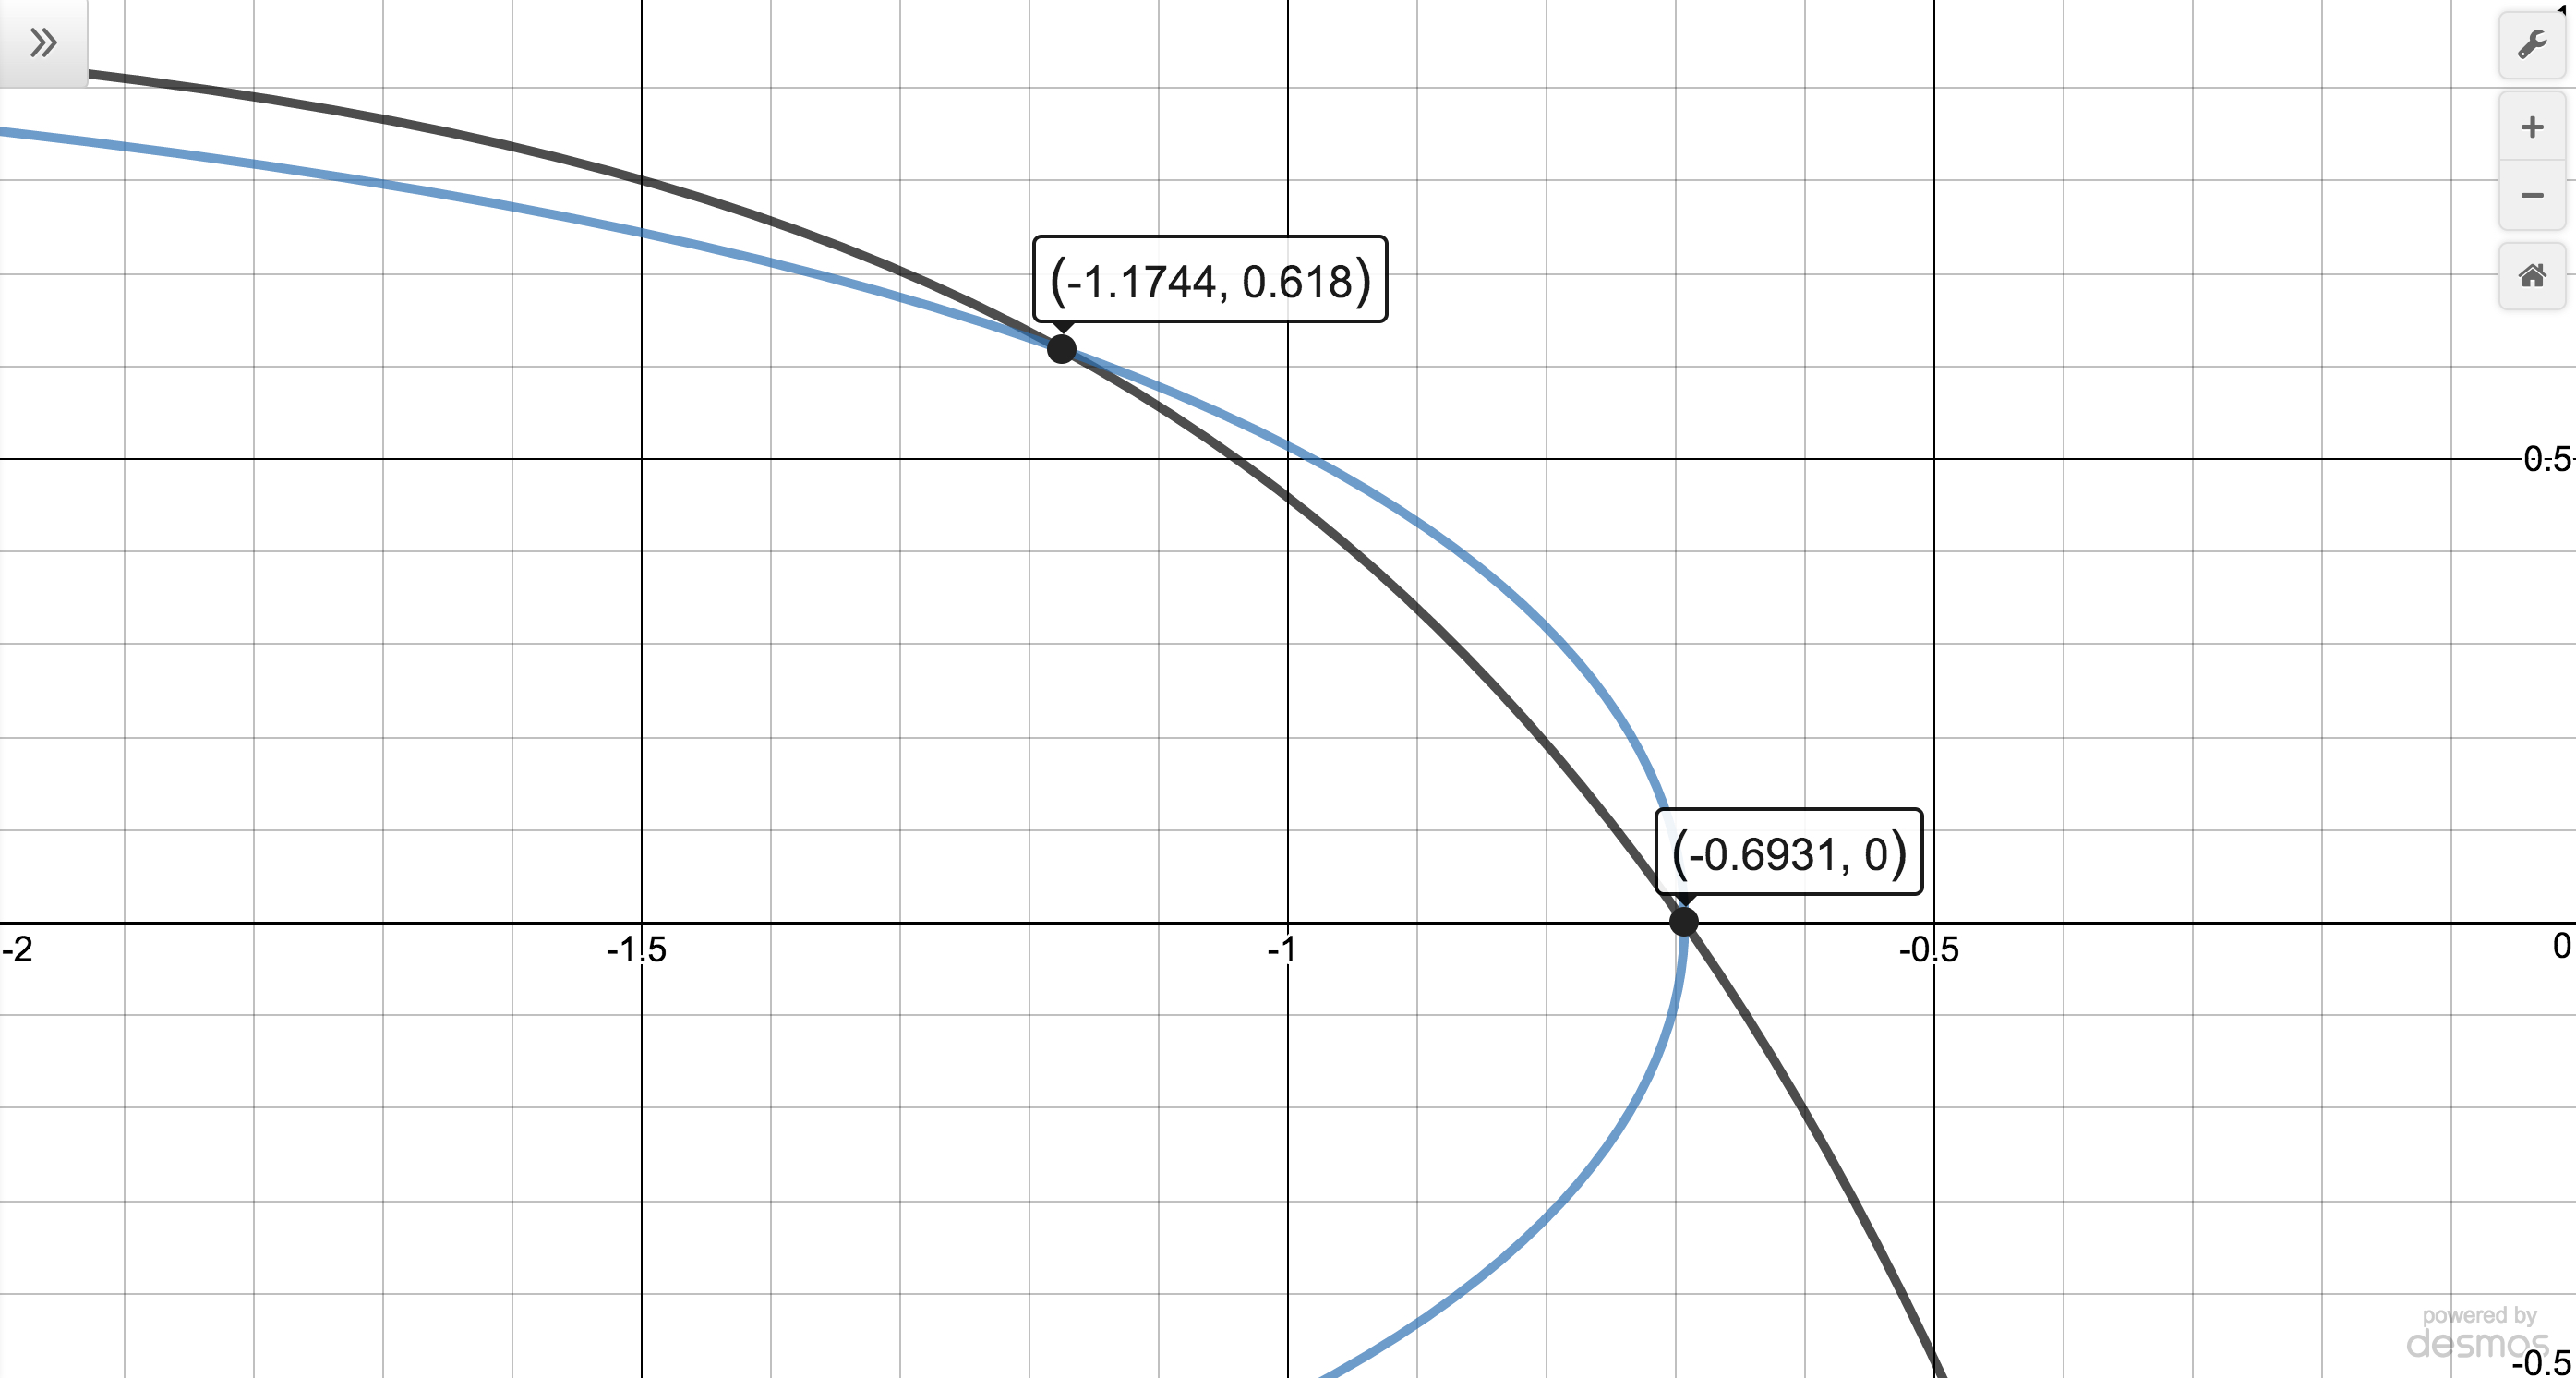
\includegraphics[width=4in]{./NonLinearEquationsGraphics/NonLinear01.jpg} 

Graphs for $\left\{\begin{array}{rcl}  y+4e^{2x} & = & 1 \\y^2 + 2e^{x} & = & 1 \\ \end{array} \right.$

\end{center}




\item  Our last system involves three variables and provides an opportunity to gain some insight on how to keep such systems organized.  Labeling the equations as before, we have

\[\left\{\begin{array}{lrcl}   E1 & z(x-2) & = & x \\ E2 & yz & = & y \\ E3 & (x-2)^2+y^2 & = & 1 \end{array} \right.\]

The easiest equation to start with appears to be $E2$.  While it may be tempting to divide both sides of $E2$ by $y$, we caution against this practice because it presupposes $y \neq 0$.  Instead, we take $E2$ and rewrite it as $yz-y = 0$ so $y(z-1) = 0$.  From this, we get two cases:  $y = 0$ or $z = 1$.

{ \sc Case 1: $y = 0$. }  Substituting $y=0$ into $E1$ and $E3$, we get 

\[\left\{\begin{array}{lrcl}   E1 & z(x-2) & = & x \\ E3 & (x-2)^2 & = & 1 \end{array} \right.\]

Solving $E3$ for $x$ gives $x = 1$ or $x=3$.  Substituting these values into $E1$ gives $z=-1$ when $x=1$ and $z = 3$ when $x=3$.  We obtain two solutions, $(1,0,-1)$ and $(3,0,3)$.

{ \sc Case 2:  $z = 1$. }  Substituting $z=1$ into $E1$ and $E3$ gives us 


\[\left\{\begin{array}{lrcl}   E1 & (1)(x-2) & = & x  \\ E3 & (x-2)^2+y^2 & = & 1 \end{array} \right.\]

Equation $E1$ gives us $x-2 = x$ or $-2 = 0$, which is a contradiction.  This means we have no solution to the system in this case, even though $E3$ is satisfied by infinitely many pairs of points $(x,y)$.  

Hence, our final answer is $\left\{ (1,0,-1), (3,0,3) \right\}$.  These points are easy enough to check algebraically in our three original equations, so that is left to the reader.  

As for verifying these solutions graphically, they require plotting surfaces in three dimensions and looking for intersection points.  While this is beyond the scope of this book, we provide a snapshot of the graphs of our three equations near one of the solution points,  $(1,0,-1)$ and $(3,0,3)$. \qed

\begin{center}

\begin{tabular}{cc}

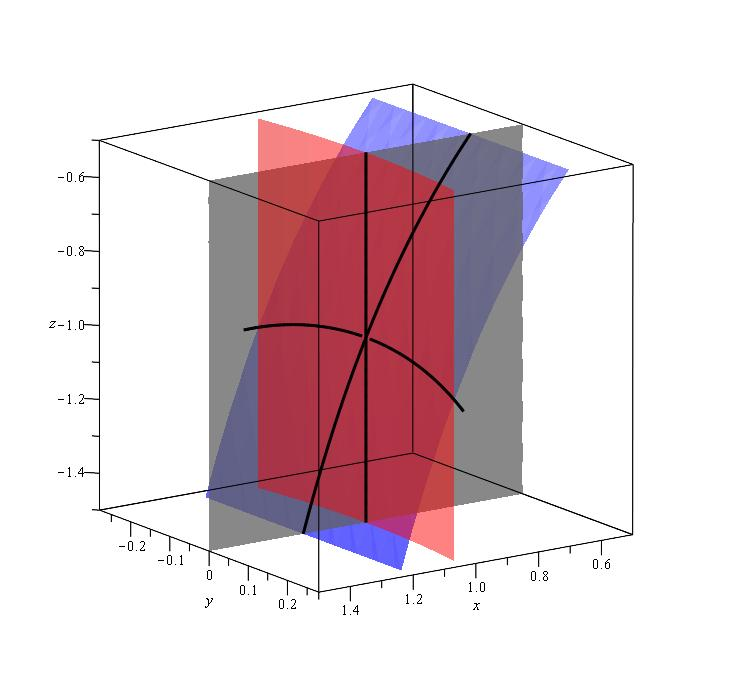
\includegraphics[height=2.25in]{./NonLinearEquationsGraphics/NonLinear03a.jpg}

&

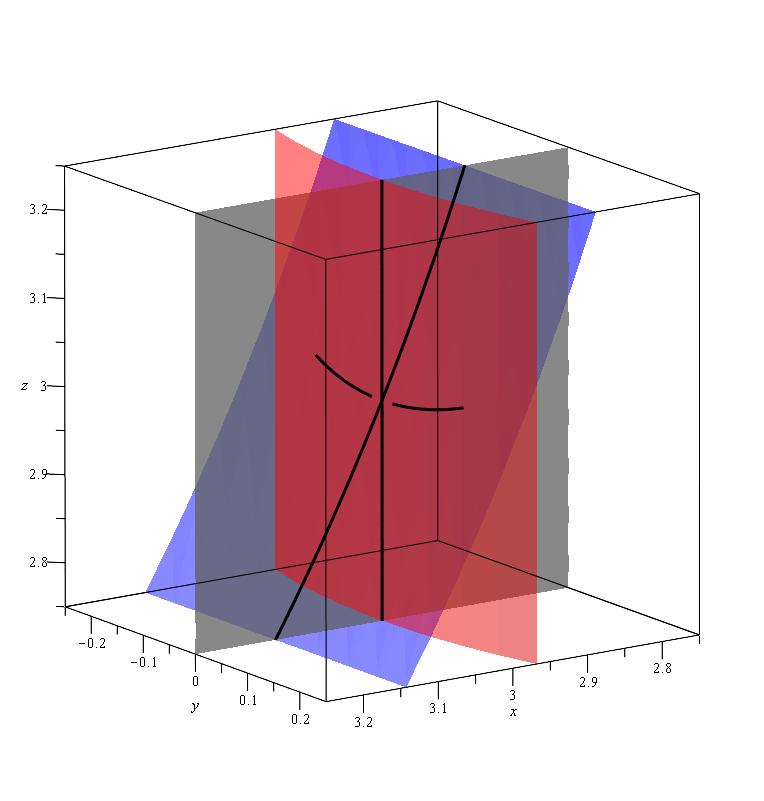
\includegraphics[height=2.25in]{./NonLinearEquationsGraphics/NonLinear03b.jpg} \\

Near $(-1,0,1)$ 

&

Near $(3,0,3)$ \\

\end{tabular}

\end{center}
\end{enumerate}


\end{ex}

Example \ref{nonlinearex2} showcases some of the ingenuity and tenacity mentioned at the beginning of the section.  Sometimes you just have to look at a system the right way to find the most efficient method to solve it.  Sometimes you just have to try something.  

\smallskip

Next we explore some common application problems which give rise to systems of nonlinear equations.

\begin{ex}  \label{upstreamdownstreamex}  Carl decides to explore the Meander River, the location of several recent Sasquatch sightings.  From camp, he canoes downstream five miles to check out a purported Sasquatch nest.  Finding nothing, he immediately turns around, retraces his route (this time traveling upstream), and returns to camp 3 hours after he left.  If Carl canoes at a rate  of 6 miles per hour in still water, how fast was the Meander River flowing on that day?

\smallskip

{\bf Solution.}  We are given information about distances, rates (speeds) and times.  The basic principle relating these quantities is: \[ \text{distance} = \text{rate} \cdot \text{time}\]  The first observation to make, however, is that the distance, rate and time given to us aren't `compatible':  the distance given is the distance for only \textit{part} of the trip,  the rate given is the speed Carl can canoe in still water, not in a flowing river, and  the time given is the duration of the \textit{entire} trip.  Ultimately, we are after the speed of the river, so let's call that $R$ measured in miles per hour to be consistent with the other rate given to us.  To get started, let's divide the trip into its two parts:  the initial trip downstream and the return trip upstream.  For the downstream trip, all we know is that the distance traveled is $5$ miles.

\[ \begin{array}{rcl}

\text{distance downstream} & = & \text{rate traveling downstream} \cdot \text{time traveling downstream} \\

5 \, \text{miles} & = & \text{rate traveling downstream} \cdot \text{time traveling downstream} \\ \end{array} \]

Since the return trip upstream followed the same route as the trip downstream, we know that the distance traveled upstream is also 5 miles.

\[ \begin{array}{rcl}

\text{distance upstream} & = & \text{rate traveling upstream} \cdot \text{time traveling upstream} \\

5 \, \text{miles} & = & \text{rate traveling upstream} \cdot \text{time traveling upstream} \\ \end{array} \]

We are told Carl can canoe at a  rate of $6$ miles per hour in still water.  How does this figure into the rates traveling upstream and downstream?  The speed the canoe travels in the river is a combination of the speed at which Carl can propel the canoe in still water, 6 miles per hour,  and the speed of the river, which we're calling $R$. When traveling downstream, the river is helping Carl along, so we \textit{add} these two speeds: 

\[ \begin{array}{rcl}

\text{rate traveling downstream} & = & \text{rate Carl propels the canoe} + \text{speed of the river} \\

 & = & 6 \frac{\text{miles}}{\text{hour}} + R \frac{\text{miles}}{\text{hour}} \\ \end{array} \]
 
 So our downstream speed is $(6+R) \frac{\text{miles}}{\text{hour}}$.  Substituting this into our `distance-rate-time' equation for the downstream part of the trip, we get:
 
 \[ \begin{array}{rcl}

5 \, \text{miles} & = & \text{rate traveling downstream} \cdot \text{time traveling downstream} \\ 

5 \, \text{miles} & = & (6+R) \frac{\text{miles}}{\text{hour}} \cdot \text{time traveling downstream} \\ 	\end{array} \]

 When traveling upstream, Carl works \textit{against} the current.  Since Carl must move the canoe faster than the river's speed to move upstream,  we \textit{subtract} the river's speed \textit{from} Carl's canoing speed to get:
 
 \[ \begin{array}{rcl}

\text{rate traveling upstream} & = & \text{rate Carl propels the canoe} - \text{river speed} \\

 & = & 6 \frac{\text{miles}}{\text{hour}} - R \frac{\text{miles}}{\text{hour}} \\ \end{array} \]
 
Proceeding as before, we get
 
 \[ \begin{array}{rcl}

5 \, \text{miles} & = & \text{rate traveling upstream} \cdot \text{time traveling upstream} \\ 

5 \, \text{miles} & = & (6 - R) \frac{\text{miles}}{\text{hour}} \cdot \text{time traveling upstream} \\ 	\end{array} \]
 
The last piece of information given to us is that the total trip lasted $3$ hours.  If we let $t_{\text{down}}$ denote the time of the downstream trip and $t_{\text{up}}$ the time of the upstream trip, we have:    $t_{\text{down}} + t_{\text{up}} = 3 \, \text{hours}$.  Substituting $t_{\text{down}}$ and $t_{\text{up}}$ into the `distance-rate-time' equations, we get a system of three equations in three unknowns below.  Note that since the variables in equations $E1$ and $E2$ are multiplied together, these two equations are nonlinear.

 \[\left\{\begin{array}{lrcl}   E1 & (6+R) \, t_{\text{down}} & = & 5 \\ E2 & (6-R) \, t_{\text{up}} & = & 5 \\ E3 & t_{\text{down}} + t_{\text{up}} & = & 3 \end{array} \right.\]

Since we are ultimately after $R$, we need to use these three equations to get at least one equation involving \textit{only} $R$.  We start with equation $E1$. We know that both $(6+R) \neq 0$  and  $t_{\text{down}} \neq 0$ since the product of these two quantities is $5$ and is nonzero.\footnote{This is a restatement of the Zero Product Property from Section \ref{AppRealNumberArithmetic}.}  Hence, we may solve $E1$ for $t_{\text{down}}$ by dividing both sides by the quantity $(6+R)$ to get $t_{\text{down}} = \frac{5}{6+R}$.   Similarly, we use $E2$  to get $t_{\text{up}} = \frac{5}{6-R}$. Substituting these into $E3$, we get:\footnote{The reader is encouraged to verify that the units in this equation are consistent. For starters, the units on the `3' is `hours.'} \[\dfrac{5}{6+R} + \dfrac{5}{6 - R} = 3.\] Clearing denominators, we get $5(6-R) + 5(6+R) = 3(6+R)(6-R)$ which reduces to  $R^2 = 16$.   We find $R = \pm 4$, and since $R$ represents the speed of the river, we choose $R = 4$.   On the day in question, the Meander River is flowing at a rate of $4$ miles per hour. \qed

\end{ex}

One of the important lessons to learn from Example \ref{upstreamdownstreamex} is that speeds, and more generally, rates, are additive.  As we see in our next example, the concept of rate and its associated principles can be applied to a wide variety of problems - not just `distance-rate-time' scenarios.

\begin{ex} \label{workex}  Working alone, Taylor can weed the garden in 4 hours.  If Carl helps, they can weed the garden in 3 hours.  How long would it take for Carl to weed the garden on his own?

\smallskip

{\bf Solution.}  The key relationship between work and time which we use in this problem is: \[\text{amount of work done} = \text{rate of work} \cdot \text{time spent working} \]

We are told that, working alone, Taylor can weed the garden in 4 hours.  In Taylor's case then: \[ \begin{array}{rcl}

\text{amount of work Taylor does} & = & \text{rate of Taylor working} \cdot \text{time Taylor spent working} \\

1 \, \text{garden} & = & (\text{rate of Taylor working}) \cdot (4 \, \text{hours}) \\ \end{array} \]

So we have that the rate Taylor works is $\frac{1 \, \text{garden}}{ 4 \, \text{hours}} = \frac{1}{4} \frac{\text{garden}}{\text{hour}}$.    We are also told that when working together, Taylor and Carl can weed the garden in just 3 hours.  We have:

\[ \begin{array}{rcl}

\text{amount of work done together} & = & \text{rate of working together} \cdot \text{time spent working together} \\

1 \, \text{garden} & = & (\text{rate of working together}) \cdot (3 \, \text{hours}) \\ \end{array} \]

From this, we find that the rate of Taylor and Carl working together is $\frac{1 \, \text{garden}}{3 \, \text{hours}} = \frac{1}{3} \frac{\text{garden}}{\text{hour}}$.   We are asked to find out how long it would take for Carl to weed the garden on his own.  Let us call this unknown $t$, measured in hours to be consistent with the other times given to us in the problem. Then:

\[ \begin{array}{rcl}

\text{amount of work Carl does} & = & \text{rate of Carl working} \cdot \text{time Carl spent working} \\

1 \, \text{garden} & = & (\text{rate of Carl working}) \cdot (t \, \text{hours}) \\ \end{array} \]

In order to find $t$, we need to find the rate of Carl working, so let's call this quantity $R$, with units $\frac{\text{garden}}{\text{hour}}$.  Using the fact that rates are additive, we have:

\[ \begin{array}{rcl}

\text{rate working together} & = & \text{rate of Taylor working} + \text{rate of Carl working} \\ [5pt]

\frac{1}{3} \frac{\text{garden}}{\text{hour}} & = & \frac{1}{4} \frac{\text{garden}}{\text{hour}} + R \frac{\text{garden}}{\text{hour}} \\ \end{array} \]

so that $R = \frac{1}{12} \frac{\text{garden}}{\text{hour}}$.  Substituting this into our `work-rate-time' equation for Carl, we get:

\[ \begin{array}{rcl}

1 \, \text{garden} & = & (\text{rate of Carl working}) \cdot (t \, \text{hours}) \\ [5pt] 

1 \, \text{garden} & = & \left(\frac{1}{12} \frac{\text{garden}}{\text{hour}} \right) \cdot (t \, \text{hours}) \\ \end{array} \]

Solving $1 = \frac{1}{12} t$, we get $t = 12$, so it takes Carl 12 hours to weed the garden on his own.\footnote{Carl would much rather spend his time writing open-source Mathematics texts than gardening anyway.} \qed

\end{ex}

As is common with `word problems' like Examples \ref{upstreamdownstreamex} and \ref{workex}, there is no short-cut to the answer.  Note that in  Examples \ref{upstreamdownstreamex}, we formalized the system of non-linear equations before solving whereas in Example \ref{workex}, the system remained much in the background.  We encourage the reader to carefully think through and apply the basic principles of rate to each (potentially different!) situation.  It is time well spent.  We also encourage the tracking of units, especially in the early stages of the problem.  Not only does this promote uniformity in the units, it also serves as a quick means to check if an equation makes sense.\footnote{In other words, make sure you don't try to add apples to oranges!}

\newpage

\subsection{Exercises}
\documentclass{ximera}

\begin{document}
	\author{Stitz-Zeager}
	\xmtitle{TITLE}
\mfpicnumber{1} \opengraphsfile{ExercisesforNonLinearEquations} % mfpic settings added 


\label{ExercisesforNonLinearEquations}

Exercise idea:  follow up on last example and have students formalize the system there using given variables.

In Exercises \ref{solvenonlin1first} - \ref{solvenonlin1last}, solve the given system of nonlinear equations.  Sketch the graph of both equations on the same set of axes to verify the solution set. 

\begin{multicols}{3}
\begin{enumerate}

\item $\left\{\begin{array}{rcr}  x^2 - y & = & 4 \\ x^{2} + y^{2} & = & 4 \\ \end{array} \right.$ \label{solvenonlin1first}
\item $\left\{\begin{array}{rcr}  x^{2} + y^{2} & = & 4 \\ x^2 - y & = & 5 \\ \end{array} \right.$
\item $\left\{\begin{array}{rcr}  x^2+y^2 & = & 16 \\ 16x^{2} + 4y^{2} & = & 64 \\ \end{array} \right.$

\setcounter{HW}{\value{enumi}}
\end{enumerate}
\end{multicols}

\begin{multicols}{3}
\begin{enumerate}
\setcounter{enumi}{\value{HW}}

\item $\left\{\begin{array}{rcr}  x^2+y^2 & = & 16 \\ 9x^{2} - 16y^{2} & = & 144 \\ \end{array} \right.$
\item $\left\{\begin{array}{rcr}  x^2+y^2 & = & 16 \\ \frac{1}{9} y^2 - \frac{1}{16} x^2& = & 1 \\ \end{array} \right.$
\item $\left\{\begin{array}{rcr}  x^{2} + y^{2} & = & 16 \\ x-y & = & 2 \\ \end{array} \right.$ \label{solvenonlin1last}

\setcounter{HW}{\value{enumi}}
\end{enumerate}
\end{multicols}

In Exercises \ref{solvenonlin2first} - \ref{solveninlin2last}, solve the given system of nonlinear equations.  Use a graph to help you avoid any potential extraneous solutions.


\begin{multicols}{3}
\begin{enumerate}
\setcounter{enumi}{\value{HW}}


\item $\left\{\begin{array}{rcr}  x^{2} - y^{2} & = & 1 \\ x^{2} + 4y^{2} & = & 4 \\ \end{array} \right.$ \label{solvenonlin2first}
\item $\left\{\begin{array}{rcr}  \sqrt{x + 1} - y & = & 0 \\ x^{2} + 4y^{2} & = & 4 \\ \end{array} \right.$
\item $\left\{\begin{array}{rcr}  x + 2y^{2} & = & 2 \\ x^{2} + 4y^{2} & = & 4 \\ \end{array} \right.$ 

\setcounter{HW}{\value{enumi}}
\end{enumerate}
\end{multicols}

\begin{multicols}{3}
\begin{enumerate}
\setcounter{enumi}{\value{HW}}

\item $\left\{\begin{array}{rcr}  (x - 2)^{2} + y^{2} & = & 1 \\ x^{2} + 4y^{2} & = & 4 \\ \end{array} \right.$
\item $\left\{\begin{array}{rcr}  x^{2} + y^{2} & = & 25 \\ y - x & = & 1 \\ \end{array} \right.$
\item $\left\{\begin{array}{rcr}  x^{2} + y^{2} & = & 25 \\ x^{2} + (y - 3)^{2} & = & 10 \\ \end{array} \right.$

\setcounter{HW}{\value{enumi}}
\end{enumerate}
\end{multicols}

\begin{multicols}{3}
\begin{enumerate}
\setcounter{enumi}{\value{HW}}

\item $\left\{\begin{array}{rcr}  y & = & x^{3} + 8 \\ y & = & 10x - x^{2} \\ \end{array} \right. \vphantom{\left\{\begin{array}{rcr}  x^{2} + y^{2} & = & 25 \\ 4x^{2} - 9y & = & 0 \\ 3y^{2} - 16x & = & 0\end{array} \right.}$

\item $\left\{\begin{array}{rcr}  x^2 - xy & = & 8 \\  y^2 - xy & = & 8 \\ \end{array} \right. \vphantom{\left\{\begin{array}{rcr}  x^{2} + y^{2} & = & 25 \\ 4x^{2} - 9y & = & 0 \\ 3y^{2} - 16x & = & 0\end{array} \right.}$

\item $\left\{\begin{array}{rcr}  x^{2} + y^{2} & = & 25 \\ 4x^{2} - 9y & = & 0 \\ 3y^{2} - 16x & = & 0\end{array} \right.$ \label{solveninlin2last}

\setcounter{HW}{\value{enumi}}
\end{enumerate}
\end{multicols}

\begin{enumerate}
\setcounter{enumi}{\value{HW}}

\item  A certain bacteria culture follows the Law of Uninbited Growth, Equation \ref{lawofuninhibitedgrowth}.  After 10 minutes, there are 10,000 bacteria. Five minutes later, there are 14,000 bacteria.  How many bacteria were present initially?  How long before there are 50,000 bacteria?


\setcounter{HW}{\value{enumi}}
\end{enumerate}


Consider the system of nonlinear equations  below \[\left\{\begin{array}{rcr}  \dfrac{4}{x} + \dfrac{3}{y} & = & 1 \\[10pt] \dfrac{3}{x} + \dfrac{2}{y} & = & -1 \\ \end{array} \right.\]  If we let $u = \frac{1}{x}$ and $v = \frac{1}{y}$ then the system becomes \[\left\{\begin{array}{rcr}  4u + 3v & = & 1 \\ 3u + 2v & = & -1 \\ \end{array} \right.\] This associated system of linear equations can then be solved using any of the techniques presented earlier in the chapter to find that $u = -5$ and $v = 7$.  Thus $x = \frac{1}{u} = -\frac{1}{5}$ and $y = \frac{1}{v} = \frac{1}{7}$.  

\smallskip

We say that the original system is {\bf linear in form} \index{system of equations ! linear in form} because its equations are not linear but a few substitutions reveal a structure that we can treat like a system of linear equations.  Each system in Exercises \ref{linearformfirst} - \ref{linearformlast}  is linear in form.  Make the appropriate substitutions and solve for $x$ and $y$.

\begin{multicols}{3}
\begin{enumerate}
\setcounter{enumi}{\value{HW}}

\item $\left\{\begin{array}{rcr}  4x^{3} + 3\sqrt{y} & = & 1 \\ 3x^{3} + 2\sqrt{y} & = & -1  \end{array} \right.$ \label{linearformfirst}
\item $\left\{\begin{array}{rcr}  4e^{x} + 3e^{-y} & = & 1 \\ 3e^{x} + 2e^{-y} & = & -1  \end{array} \right.$
\item $\left\{\begin{array}{rcr}  4\ln(x) + 3y^{2} & = & 1 \\ 3\ln(x) + 2y^{2} & = & -1 \end{array} \right.$ \label{linearformlast}

\setcounter{HW}{\value{enumi}}
\end{enumerate}
\end{multicols}

\begin{enumerate}
\setcounter{enumi}{\value{HW}}

\item Solve the following system \[\left\{\begin{array}{rcr}  x^{2} + \sqrt{y} + \log_{2}(z) & = & 6 \\[3pt] 3x^{2} - 2\sqrt{y} + 2\log_{2}(z) & = & 5 \\[3pt] -5x^{2} + 3\sqrt{y} + 4\log_{2}(z) & = & 13 \end{array} \right.\]

\setcounter{HW}{\value{enumi}}
\end{enumerate}

\begin{enumerate}
\setcounter{enumi}{\value{HW}}


\item Systems of nonlinear equations show up in third semester Calculus in the midst of some really cool problems.  The system below came from a problem in which we were asked to find the dimensions of a rectangular box with a volume of 1000 cubic inches that has minimal surface area.  The variables $x$, $y$ and $z$ are the dimensions of the box and $\lambda$ is called a Lagrange multiplier.  With the help of your classmates, solve the system.\footnote{If using $\lambda$ bothers you, change it to $w$ when you solve the system.} \[\left\{\begin{array}{rcr}  2y + 2z & = & \lambda yz  \\ 2x + 2z & = & \lambda xz \\ 2y + 2x & = & \lambda xy \\ xyz & = & 1000 \end{array} \right.\]

\item According to Theorem \ref{realfactorization} in Section \ref{ComplexZeros}, the polynomial $p(x) = x^{4} + 4$ can be factored into the product linear and irreducible quadratic factors.  In this exercise, we present a method for obtaining that factorization.  
\label{factorpolywithnonlinear}

\begin{enumerate}

\item Show that $p$ has no real zeros.  

\item Because $p$ has no real zeros, its factorization must be of the form $(x^{2} + ax + b)(x^{2} + cx + d)$ where each factor is an irreducible quadratic.  Expand this quantity and gather like terms together.

\item Create and solve the system of nonlinear equations which results from equating the coefficients of the expansion found above with those of $x^{4} + 4$.  You should get four equations in the four unknowns $a$, $b$, $c$ and $d$.  Write $p(x)$ in factored form.

\end{enumerate}

\item Factor $q(x) = x^{4} + 6x^{2} - 5x + 6$.

\end{enumerate}

\newpage

\subsection{Answers}

\begin{multicols}{2}
\begin{enumerate}

\item $(\pm 2, 0)$, $\left(\pm \sqrt{3}, -1\right)$ \\
\begin{mfpic}[15]{-3}{3}{-5}{3}
\arrow \reverse \arrow \function{-2.5,2.5,0.1}{x**2 - 4}
\circle{(0,0),2}
\point[3pt]{(2,0), (-2,0), (1.7320,-1), (-1.7320,-1)}
\axes
\tlabel[cc](3,-0.5){\scriptsize $x$}
\tlabel[cc](0.5,3){\scriptsize $y$}
\xmarks{-2,-1,1,2}
\ymarks{-4,-3,-2,-1,1,2}
\tlpointsep{4pt}
\tiny
\axislabels {x}{{$-2 \hspace{7pt}$} -2, {$-1 \hspace{7pt}$} -1, {$1$} 1, {$2$} 2}
\axislabels {y}{{$-4$} -4,{$-3$} -3,{$-2$} -2, {$-1$} -1, {$1$} 1, {$2$} 2}
\normalsize
\end{mfpic}

\vfill

\columnbreak

\item No solution \\

\begin{mfpic}[15]{-3}{3}{-6}{3}
\arrow \reverse \arrow \function{-2.75,2.75,0.1}{x**2 - 5}
\circle{(0,0),2}
\axes
\tlabel[cc](3,-0.5){\scriptsize $x$}
\tlabel[cc](0.5,3){\scriptsize $y$}
\xmarks{-2,-1,1,2}
\ymarks{-4,-3,-2,-1,1,2}
\tlpointsep{4pt}
\tiny
\axislabels {x}{{$-2 \hspace{7pt}$} -2, {$-1 \hspace{7pt}$} -1, {$1$} 1, {$2$} 2}
\axislabels {y}{{$-4$} -4,{$-3$} -3,{$-2$} -2, {$-1$} -1, {$1$} 1, {$2$} 2}
\normalsize
\end{mfpic}

\setcounter{HW}{\value{enumi}}
\end{enumerate}
\end{multicols}

\begin{multicols}{2}
\begin{enumerate}
\setcounter{enumi}{\value{HW}}

\item  $(0, \pm 4)$ \\
\begin{mfpic}[10]{-5}{5}{-5}{5}
\ellipse{(0,0), 2, 4}
\circle{(0,0),4}
\point[3pt]{(0,4), (0,-4)}
\axes
\tlabel[cc](5,-0.5){\scriptsize $x$}
\tlabel[cc](0.5,5){\scriptsize $y$}
\xmarks{-4,-3,-2,-1,1,2,3,4}
\ymarks{-4,-3,-2,-1,1,2,3,4}
\tlpointsep{4pt}
\tiny
\axislabels {x}{{$-4 \hspace{7pt}$} -4,{$-3 \hspace{7pt}$} -3,{$-2 \hspace{7pt}$} -2, {$-1 \hspace{7pt}$} -1, {$1$} 1, {$2$} 2, {$3$} 3, {$4$} 4}
\axislabels {y}{{$-4$} -4,{$-3$} -3,{$-2$} -2, {$-1$} -1, {$1$} 1, {$2$} 2, {$3$} 3, {$4$} 4}
\normalsize
\end{mfpic}

\vfill

\columnbreak

\item  $(\pm 4,0)$ \\
\begin{mfpic}[10]{-7}{7}{-5}{5}
\arrow \reverse \arrow \parafcn{-1, 1,0.1}{(4*cosh(t), 3*sinh(t))}
\arrow \reverse \arrow \parafcn{-1, 1,0.1}{(0-4*cosh(t), 3*sinh(t))}
\circle{(0,0),4}
\point[3pt]{(4,0), (-4,0)}
\axes
\tlabel[cc](7,-0.5){\scriptsize $x$}
\tlabel[cc](0.5,5){\scriptsize $y$}
\xmarks{-6,-5,-4,-3,-2,-1,1,2,3,4,5,6}
\ymarks{-4,-3,-2,-1,1,2,3,4}
\tlpointsep{4pt}
\tiny
\axislabels {x}{{$-6 \hspace{7pt}$} -6,{$-5 \hspace{7pt}$} -5,{$-4 \hspace{7pt}$} -4,{$-3 \hspace{7pt}$} -3,{$-2 \hspace{7pt}$} -2, {$-1 \hspace{7pt}$} -1, {$1$} 1, {$2$} 2, {$3$} 3, {$4$} 4, {$5$} 5, {$6$} 6}
\axislabels {y}{{$-4$} -4,{$-3$} -3,{$-2$} -2, {$-1$} -1, {$1$} 1, {$2$} 2, {$3$} 3, {$4$} 4}
\normalsize
\end{mfpic}


\setcounter{HW}{\value{enumi}}
\end{enumerate}
\end{multicols}

\begin{multicols}{2}
\begin{enumerate}
\setcounter{enumi}{\value{HW}}

\item  $\left(\pm \frac{4 \sqrt{7}}{5}, \pm \frac{12 \sqrt{2}}{5}  \right)$ \\
\begin{mfpic}[10]{-5}{5}{-5}{5}
\arrow \reverse \arrow \parafcn{-1, 1,0.1}{(4*sinh(t), 3*cosh(t))}
\arrow \reverse \arrow \parafcn{-1, 1,0.1}{(4*sinh(t), 0-3*cosh(t))}
\circle{(0,0),4}
\point[3pt]{(2.1166,3.3941), (2.1166, -3.3941), (-2.1166,3.3941), (-2.1166,-3.3941) }
\axes
\tlabel[cc](5,-0.5){\scriptsize $x$}
\tlabel[cc](0.5,5){\scriptsize $y$}
\xmarks{-4,-3,-2,-1,1,2,3,4}
\ymarks{-4,-3,-2,-1,1,2,3,4}
\tlpointsep{4pt}
\tiny
\axislabels {x}{{$-4 \hspace{7pt}$} -4,{$-3 \hspace{7pt}$} -3,{$-2 \hspace{7pt}$} -2, {$-1 \hspace{7pt}$} -1, {$1$} 1, {$2$} 2, {$3$} 3, {$4$} 4}
\axislabels {y}{{$-4$} -4,{$-3$} -3,{$-2$} -2, {$-1$} -1, {$1$} 1, {$2$} 2, {$3$} 3, {$4$} 4}
\normalsize
\end{mfpic}

\vfill

\columnbreak

\item  $\left( 1 + \sqrt{7}, -1 + \sqrt{7}  \right)$, $\left( 1 - \sqrt{7}, -1 - \sqrt{7}  \right)$ \\
\begin{mfpic}[10]{-5}{5}{-5}{5}
\arrow \reverse \arrow \function{-3,5,0.1}{x-2}
\circle{(0,0),4}
\point[3pt]{(3.6458,1.6458), (-1.6458, -3.6458) }
\axes
\tlabel[cc](5,-0.5){\scriptsize $x$}
\tlabel[cc](0.5,5){\scriptsize $y$}
\xmarks{-4,-3,-2,-1,1,2,3,4}
\ymarks{-4,-3,-2,-1,1,2,3,4}
\tlpointsep{4pt}
\tiny
\axislabels {x}{{$-4 \hspace{7pt}$} -4,{$-3 \hspace{7pt}$} -3,{$-2 \hspace{7pt}$} -2, {$-1 \hspace{7pt}$} -1, {$1$} 1, {$2$} 2, {$3$} 3, {$4$} 4}
\axislabels {y}{{$-4$} -4,{$-3$} -3,{$-2$} -2, {$-1$} -1, {$1$} 1, {$2$} 2, {$3$} 3, {$4$} 4}
\normalsize
\end{mfpic}

\setcounter{HW}{\value{enumi}}
\end{enumerate}
\end{multicols}

\begin{multicols}{3}
\begin{enumerate}
\setcounter{enumi}{\value{HW}}

\item $\left( \pm \frac{2 \sqrt{10}}{5}, \pm \frac{\sqrt{15}}{5} \right)$
\item $(0, 1)$
\item $(0, \pm 1), \; (2, 0)$


\setcounter{HW}{\value{enumi}}
\end{enumerate}
\end{multicols}

\begin{multicols}{3}
\begin{enumerate}
\setcounter{enumi}{\value{HW}}
\item $\left( \frac{4}{3}, \pm \frac{\sqrt{5}}{3} \right)$
\item $(3, 4), \; (-4, -3)$
\item $(\pm 3, 4)$
\setcounter{HW}{\value{enumi}}
\end{enumerate}
\end{multicols}

\begin{multicols}{3}
\begin{enumerate}
\setcounter{enumi}{\value{HW}}

\item $(-4, -56), \; (1, 9), \; (2, 16)$
\item $(-2,2)$, $(2,-2)$
\item $(3, 4)$

\setcounter{HW}{\value{enumi}}
\end{enumerate}
\end{multicols}


\begin{enumerate}
\setcounter{enumi}{\value{HW}}

\item  Initially, there are $\frac{250000}{49} \approx 5102$ bacteria.  It will take $\frac{5\ln(49/5)}{\ln(7/5)} \approx 33.92$ minutes for the colony to grow to 50,000 bacteria.

\setcounter{HW}{\value{enumi}}
\end{enumerate}


\begin{multicols}{3}
\begin{enumerate}
\setcounter{enumi}{\value{HW}}

\item $\left( -\sqrt[3]{5}, 49 \right)$
\item No solution
\item $\left( e^{-5}, \pm \sqrt{7} \right)$

\setcounter{HW}{\value{enumi}}
\end{enumerate}
\end{multicols}

\begin{enumerate}
\setcounter{enumi}{\value{HW}}

\item $(1, 4, 8), \; (-1, 4, 8)$


\setcounter{HW}{\value{enumi}}
\end{enumerate}

\begin{enumerate}
\setcounter{enumi}{\value{HW}}

\item $x = 10, \; y = 10, \; z = 10, \lambda = \frac{2}{5}$

\setcounter{HW}{\value{enumi}}
\end{enumerate}

\begin{enumerate}
\setcounter{enumi}{\value{HW}}

\item \begin{enumerate} 

\addtocounter{enumii}{2}

\item $x^{4} + 4 = (x^{2} - 2x + 2)(x^{2} + 2x + 2)$

\end{enumerate}

\item $x^{4} + 6x^{2} - 5x + 6 = (x^{2} - x + 1)(x^{2} + x + 6)$

\end{enumerate}


\end{document}


\closegraphsfile

\end{document}


\newpage

\section{Inequalities and Regions in the Plane}

\documentclass{ximera}

\begin{document}
	\author{Stitz-Zeager}
	\xmtitle{TITLE}


\mfpicnumber{1}

\opengraphsfile{NonLinearInequalities}

\setcounter{footnote}{0}

\label{NonLinearInequalities}

With few exceptions, we have spent our time in this course graphing equations relating two variables.  In this section, we explore graphing inequalities relating two variables which  usually a two-dimensional \textit{region} in the plane instead of a one dimensional line or curve.\footnote{We have \textit{some} experience describing simple regions in the plane using inequalities from our work in Section \ref{Relations}.}  In our first example, we restrict our attention to looking at regions in the $xy$-plane bounded by equations which describe $y$ as a function of $x$.

\begin{example}  \label{ineqgraphex01} $~$


\begin{enumerate}

\item Sketch the following sets of points in the $xy$-plane.


\begin{multicols}{2}

\begin{enumerate}

\item $R = \{ (x,y) \, | \,  y > |x| \}$

\item $S = \{ (x,y)  \, | \,   y \leq 6-x^2 \}$

\setcounter{HW}{\value{enumii}}

\end{enumerate}

\end{multicols}

\begin{enumerate}

\setcounter{enumii}{\value{HW}}
\item $T = \{ (x,y)  \, | \,   |x| < y \leq 6 -x^2 \}$

\end{enumerate}

\item  \label{describeregionex} Find a set builder description for each of the following regions described below:

\begin{enumerate}

\item \label{parabolalineregionex} The region graphed below:

\begin{center}

\begin{mfpic}[20]{-4}{4}{-1}{5}
\fillcolor[gray]{.7}
\gfill \btwnfcn{-1,2,0.1}{x**2}{x+2}
\axes
\tlabel[cc](4,-0.5){\scriptsize $x$}
\tlabel[cc](0.5,5){\scriptsize $y$}
\gclear \tlabelrect(0,3){\scriptsize $y=x+2$ \vphantom{ $\frac{x^2}{x^2}$} }
%\tlabel[cc](-2,1){\scriptsize $(-1,1)$}
%\tlabel[cc](2.75,4){\scriptsize $(2,4)$}
\tlabel[cc](2.5,2){\scriptsize $y=x^2$}
\xmarks{-3 step 1 until 3}
\ymarks{1, 2, 4}
\tcaption{\scriptsize The region  $R$}
\scriptsize
\tlpointsep{4pt}
\axislabels {x}{{$-3 \hspace{7pt}$} -3,{$-2 \hspace{7pt}$} -2,{$-1 \hspace{7pt}$} -1,{$1$} 1,{$2$} 2,{$3$} 3}
\axislabels {y}{{$1$} 1,{$2$} 2,{$4$} 4}
\normalsize 
\gfill \btwnfcn{0.5,2,0.1}{x**2}{x+2}
\penwd{1.25pt}
\function{-1,2,0.1}{x**2}
\function{-1,2,0.1}{x+2}
\point[4pt]{(-1,1), (2,4)}
\end{mfpic}

\end{center}

\item  The region $S$ between the graphs\footnote{sometimes written as `the region bounded by the graphs' \ldots} of $f(x) = x^3-3x$ and $g(x) = x$.


\end{enumerate}


\end{enumerate}

{\bf Solution.}  

\begin{enumerate}

\item 

\begin{enumerate}

\item  The set $R$ consists of all points $(x,y)$ whose $y$-coordinate is greater than $|x|$.  If we graph $y=|x|$, we get the familiar `$\vee$' shape with vertex at $(0,0)$.  Hence, in order for an ordered pair $(x,y)$ to satisfy  $y > |x|$,  the point $(x,y)$ must be \textit{above} the graph of $y = |x|$.  

Since the inequality here, $y > |x|$ is strict, we use a dashed line with which to indicate the graph of  $y=|x|$ and shade the region above, or `inside,' the `$\vee$' as shown below on the left.  

Note that one way to check our answer is to choose points both inside and outside the shaded region to verify the inequality either holds or it doesn't, respectively.

\item  Using the same reasoning as above we note a point $(x,y)$ is in  $S$ if its  $y$-coordinate is less than or equal to the $y$-coordinate on the parabola $y=6-x^2$.  Hence, we graph the points  \textit{below} the parabola ($y < 6-x^2$) along with the points \textit{on} the parabola ($y=6-x^2$)  below on the right.

\begin{center}

\begin{tabular}{m{3in}m{3in}}

\begin{mfpic}[15]{-7}{7}{-2}{7}
\fillcolor[gray]{.7}
\gfill \btwnfcn{-6.75,0,0.1}{-x+0.01}{6.75}
\gfill \btwnfcn{0,6.75,0.1}{x+0.01}{6.75}
\axes
\tlabel[cc](7,-0.5){\scriptsize $x$}
\tlabel[cc](0.5,7){\scriptsize $y$}
\xmarks{-6 step 1 until 6}
\ymarks{-1 step 1 until 6}
\tcaption{\scriptsize $R = \{ (x,y) : y > |x| \}$}
\scriptsize
\tlpointsep{4pt}
\axislabels {x}{{$-6 \hspace{7pt}$} -6,{$-5 \hspace{7pt}$} -5,{$-4 \hspace{7pt}$} -4,{$-3 \hspace{7pt}$} -3,{$-2 \hspace{7pt}$} -2,{$-1 \hspace{7pt}$} -1,{$1$} 1,{$2$} 2,{$3$} 3,{$4$} 4,{$5$} 5,{$6$} 6}
\axislabels {y}{{$-1$} -1,{$1$} 1,{$2$} 2,{$3$} 3,{$4$} 4,{$5$} 5,{$6$} 6}
\normalsize 
\penwd{1.25pt}
\arrow \reverse \arrow \dashed \polyline{(-7,7),(0,0),(7,7)}
\end{mfpic} \hspace{2.5in} & 

\begin{mfpic}[15]{-7}{7}{-2}{7}
\fillcolor[gray]{.7}
\gfill \btwnfcn{-2.82,2.82,0.1}{6-(x**2)}{-1.75}
\axes
\tlabel[cc](7,-0.5){\scriptsize $x$}
\tlabel[cc](0.5,7){\scriptsize $y$}
\xmarks{-6 step 1 until 6}
\ymarks{-1 step 1 until 6}
\tcaption{\scriptsize $S = \{ (x,y) :  y \leq 2-x^2 \}$}
\scriptsize
\tlpointsep{4pt}
\axislabels {x}{{$-6 \hspace{7pt}$} -6,{$-5 \hspace{7pt}$} -5,{$-4 \hspace{7pt}$} -4,{$-3 \hspace{7pt}$} -3,{$-2 \hspace{7pt}$} -2,{$-1 \hspace{7pt}$} -1,{$1$} 1,{$2$} 2,{$3$} 3,{$4$} 4,{$5$} 5,{$6$} 6}
\axislabels {y}{{$-1$} -1,{$1$} 1,{$2$} 2,{$3$} 3,{$4$} 4,{$5$} 5,{$6$} 6.25}
\normalsize 
\penwd{1.25pt}
\arrow \reverse \arrow \function{-2.82,2.82,0.1}{6-(x**2)}

\end{mfpic} \\

\end{tabular}

\end{center}

\item For a point $(x,y)$ to be in $T$, the $y$-coordinate must satisfy $|x| < y \leq 6-x^2$ which means it must belong to both $R$ and $S$.\footnote{Said differently, $T$ is the set-theoretic intersection of $R$ and $S$, $T = R \cap S$ as described in \ref{AppSetTheory}.} Thus we shade the region \textit{between} $y=|x|$ and $y=6-x^2$, keeping those points on the parabola, but not the points on $y=|x|$.  

To get an accurate graph, we need to find where these two graphs intersect, so we set $|x| = 6-x^2$.  Using the techniques discussed in Sections \ref{AbsoluteValueFunctions} and \ref{QuadraticFunctions}, we find  $x=-2,2$.  To find the associated $y$-coordinates of the intersection points, we substitute $x= \pm 2$ into either $y = |x|$ or $y = 6-x^2$ (or both, to check!)  In both cases, we find the associated $y$-coordinate  to be $2$, so the intersection points are $(-2,2)$ and $(2,2)$.  On our graph, however, these are the location of `holes' owing to the strictness of the inequality $y > |x|$.

\begin{center}

\begin{mfpic}[15]{-7}{7}{-2}{7}
\fillcolor[gray]{.7}
\gfill \btwnfcn{-2,0,0.1}{-x+0.01}{6-(x**2)}
\gfill \btwnfcn{0,2,0.1}{x+0.01}{6-(x**2)}
\axes
\tlabel[cc](7,-0.5){\scriptsize $x$}
\tlabel[cc](0.5,7){\scriptsize $y$}
\tlabel[cc](3,2){\scriptsize $(2,2)$}
\tlabel[cc](-3.25,2){\scriptsize $(-2,2)$}
\xmarks{-6 step 1 until 6}
\ymarks{-1 step 1 until 6}
\tcaption{\scriptsize $T = \{ (x,y) : |x| < y \leq 6 -x^2 \}$}
\scriptsize
\tlpointsep{4pt}
\axislabels {x}{{$-6 \hspace{7pt}$} -6,{$-5 \hspace{7pt}$} -5,{$-4 \hspace{7pt}$} -4,{$-3 \hspace{7pt}$} -3,{$-2 \hspace{7pt}$} -2,{$-1 \hspace{7pt}$} -1,{$1$} 1,{$2$} 2,{$3$} 3,{$4$} 4,{$5$} 5,{$6$} 6}
\axislabels {y}{{$-1$} -1,{$1$} 1,{$2$} 2,{$3$} 3,{$4$} 4,{$5$} 5,{$6$} 6.25}
\normalsize 
\penwd{1.25pt}
\function{-2,2,0.1}{6-(x**2)}
\dashed \polyline{(-2,2),(0,0),(2,2)}
\pointfillfalse
\point[4pt]{(-2,2), (2,2)}

\end{mfpic}

\end{center}

\end{enumerate}


\item

\begin{enumerate}

\item  Verbally, we may describe $R$ as the region \textit{between} the graphs of $y = x^2$ and $y = x+2$.  More specifically, $R$ is the set of points \textit{above} (or on) the parabola  $y=x^2$ but \textit{below} (or on) the line $y = x+2$.  That is, for the points $(x,y)$ in $R$, we have $x^2 \leq y \leq x+2$.  

To find the restrictions on $x$, we find the intersection of the graphs.  Solving $x^2 = x+2$ gives $x = -1$ and $x = 2$.  Hence, to be in $R$, points $(x,y)$ need to satisfy $-1 \leq x \leq 2$.  Hence, one way to describe $R$ is $R = \{ (x,y)  \, | \,  -1 \leq x \leq 2, \,  x^2 \leq y \leq x+2 \}$.

While this answer is correct, the fact that the line and the parabola intersect only twice producing only \textit{one} region where the inequality  $x^2 \leq y \leq x+2$ is true,  we may shorten our description of $R$ to just  $R = \{ (x,y)  \, | \,   x^2 \leq y \leq x+2 \}$.  

\item  Since we are given a verbal description of $S$, we first sketch the graph to get a sense of the geometric situation.  To graph $f(x) = x^3-3x$, we use what we learned in Section \ref{GraphsofPolynomials}:  end behavior, behavior near the $x$-intercepts, and symmetry.  The graph of $g(x) = x$ is a line with slope $1$ through the origin.

Graphing both of these functions on the same pair of axes, we see three intersection points.  Solving $f(x) = g(x)$, that is $x^3-3x = x$ gives $x = 0$ and  $x = \pm 2$.  These solutions correspond to the intersection points $(-2,-2)$, $(0,0)$, and $(2,2)$.    $S$ is described as the region `\textit{between}' these graphs, so we shade between the graphs accordingly.



\begin{center}

\begin{mfpic}[15]{-5}{5}{-5}{5}
\fillcolor[gray]{.7}
\gfill \btwnfcn{-2,0,0.1}{(x**3)-(3*x)}{x}
\gfill \btwnfcn{0,2,0.1}{x}{(x**3)-(3*x)}
\axes
\tlabel[cc](5,-0.5){\scriptsize $x$}
\tlabel[cc](0.5,5){\scriptsize $y$}
\tlabel[cc](3,2){\scriptsize $(2,2)$}
\tlabel[cc](-3.5, -2){\scriptsize $(-2,-2)$}
\xmarks{-4 step 1 until 4}
\ymarks{-4 step 1 until 4}
\tcaption{\scriptsize Graphing $f(x) = x^3-3x$ and $g(x) = x$}
\scriptsize
\tlpointsep{4pt}
\axislabels {x}{{$-4 \hspace{7pt}$} -4,{$-3 \hspace{7pt}$} -3,{$-2 \hspace{7pt}$} -2,{$-1 \hspace{7pt}$} -1,{$1$} 1,{$2$} 2,{$3$} 3,{$4$} 4}
\axislabels {y}{{$-4$} -4,{$-3$} -3,{$-2$} -2,{$-1$} -1,{$2$} 2,{$3$} 3,{$4$} 4}
\normalsize 
\penwd{1.25pt}
\arrow \reverse \arrow \function{-2.2,2.2,0.1}{(x**3)-(3*x)}
\arrow \reverse \arrow \polyline{(-4.5,-4.5),(4.5, 4.5)}
\point[4pt]{(-2,-2), (0,0), (2,2)}

\end{mfpic}

\end{center}

From the graph, we see that for $-2 < x < 0$,  the graph of $f$ is above the graph of $g$.  Algebraically, this means that for all $x$ with $-2 \leq x \leq 0$, $f(x) \geq g(x)$ or $x^3-3x \geq x$.  At $x=0$, the situation changes and we have $f(x) \leq g(x)$ or $x^3-3x \leq x$ for $0 \leq x \leq 2$.  One to describe $S$ is to describe each of these pieces and take their set theoretic union. 

We first consider the piece for $-2 \leq x \leq 0$. Unlike the previous problem, we cannot completely describe this region in terms of the $y$-values since there are \textit{two} regions where $x \leq y \leq x^3-3x$ is true:  one where $-2 \leq x \leq 0$ (the one we want) and one here $x \geq 2$ (which we don't want.) Hence, we describe this first piece as $ \{ (x,y) \, | \, -2 \leq x \leq 0, \, x \leq y \leq x^3-3x \}$.  Following this methodology for the second piece, we obtain the complete description for $S$ below: 

    \[ S = \{ (x,y) \, | \, -2 \leq x \leq 0, \, x \leq y \leq x^3-3x \} \cup\{ (x,y) \, | \, 0 \leq x \leq 2, \, x^3-3x \leq y \leq x \}. \]


\qed

\end{enumerate}

\end{enumerate}

\end{example}

A few remarks about Example \ref{ineqgraphex01} are in order.  First note that each of the regions presented here can be views as graphs of relations as described in Section \ref{Relations}.  Moreover, there are many ways to describe a region so our answers to number \ref{describeregionex} above are by no means unique.

In particular, our solution $R = \{ (x,y)  \, | \,  -1 \leq x \leq 2, \,  x^2 \leq y \leq x+2 \}$ to number  \ref{parabolalineregionex} can be visualized as `filling up' the region $R$ from the bottom curve, $y = x^2$ to the top curve, $y = x+2$ as $x$ runs from the leftmost extent of the region at $x = -1$ to the rightmost extent at $x = 2$ as indicated below. The notion that each $x$ determines where to start and stop filling the region is a consequence of us viewing the bounding curves as functions of $x$.  That is, for each $x$, we can determine the lower boundary of the region, $y = x^2$ and the upper boundary of the region, $y = x+2$.

\begin{center}

\begin{tabular}{ccc}

\begin{mfpic}[20]{-4}{4}{-1}{5}
\axes
\tlabel[cc](4,-0.5){\scriptsize $x$}
\tlabel[cc](0.5,5){\scriptsize $y$}
\tlabel[cc](-2,1){\scriptsize $(-1,1)$}
\tlabel[cc](2.75,4){\scriptsize $(2,4)$}
\xmarks{-3 step 1 until 3}
\ymarks{1, 2, 3, 4}
\tcaption{\scriptsize `Filling up'  $R$ from bottom to top.}
\scriptsize
\tlpointsep{4pt}
\axislabels {x}{{$-3 \hspace{7pt}$} -3,{$-2 \hspace{7pt}$} -2,{$-1 \hspace{7pt}$} -1,{$1$} 1,{$2$} 2,{$3$} 3}
\axislabels {y}{ {$2$} 2, {$3$} 3,{$4$} 4}
\normalsize 
\arrow \polyline{ (-0.75, 0.5625), (-0.75, 1.15)}
\arrow \polyline{ (-0.5, 0.25), (-0.5, 1.4)}
\arrow \polyline{ (-0.25, 0.0625), (-0.25, 1.65)}
\arrow \polyline{ (0, 0), (0,1.8)}
\arrow \polyline{ (0.25, 0.0625), (0.25, 2.15)}
\arrow \polyline{ (0.5, 0.25), (0.5,2.4)}
\arrow \polyline{ (0.75, 0.5625), (0.75, 2.65)}
\arrow \polyline{ (1, 1), (1,2.9)}
\arrow \polyline{ (1.25, 1.5625), (1.25,3.15)}
\arrow \polyline{ (1.5, 2.25), (1.5,3.4)}
\arrow \polyline{ (1.75,3.0625), (1.75,3.65)}
\penwd{1.25pt}
\function{-1,2,0.1}{x**2}
\function{-1,2,0.1}{x+2}
\point[4pt]{(-1,1), (2,4)}
\end{mfpic}

&

$\xrightarrow{\hspace{0.5in}}$

&

\begin{mfpic}[20]{-4}{4}{-1}{5}
\fillcolor[gray]{.7}
\gfill \btwnfcn{-1,2,0.1}{x**2}{x+2}
\axes
\tlabel[cc](4,-0.5){\scriptsize $x$}
\tlabel[cc](0.5,5){\scriptsize $y$}
\gclear \tlabelrect(0,3){\scriptsize $y=x+2$ \vphantom{ $\frac{x^2}{x^2}$} }
%\tlabel[cc](-2,1){\scriptsize $(-1,1)$}
%\tlabel[cc](2.75,4){\scriptsize $(2,4)$}
\tlabel[cc](2.5,2){\scriptsize $y=x^2$}
\xmarks{-3 step 1 until 3}
\ymarks{1, 2, 4}
\tcaption{\scriptsize The region $R$.}
\scriptsize
\tlpointsep{4pt}
\axislabels {x}{{$-3 \hspace{7pt}$} -3,{$-2 \hspace{7pt}$} -2,{$-1 \hspace{7pt}$} -1,{$1$} 1,{$2$} 2,{$3$} 3}
\axislabels {y}{{$1$} 1,{$2$} 2,{$4$} 4}
\normalsize 
\gfill \btwnfcn{0.5,2,0.1}{x**2}{x+2}
\penwd{1.25pt}
\function{-1,2,0.1}{x**2}
\function{-1,2,0.1}{x+2}
\point[4pt]{(-1,1), (2,4)}
\end{mfpic} \\

\end{tabular}

\end{center}

There are times in Calculus where it may be convenient to describe the region $R$ as filling up left-to-right as $y$ varies from the bottom most extent, $y = 0$ to the top most extent, $y = 4$.  In this case, we need to describe the bounding curves as functions of $y$.  To that end, we solve $y = x+2$ and $y = x^2$ for $x$ and get three functions of $y$:  $x = y-2$, $x = \sqrt{y}$ and $x = -\sqrt{y}$ as labeled below.

\begin{tabular}{ccc}

\begin{mfpic}[20]{-4}{4}{-1}{5}
\axes
\tlabel[cc](4,-0.5){\scriptsize $x$}
\tlabel[cc](0.5,5){\scriptsize $y$}
\tlabel[cc](-2,1){\scriptsize $(-1,1)$}
\tlabel[cc](0.5,-0.5){\scriptsize $(0,0)$}
\tlabel[cc](2.75,4){\scriptsize $(2,4)$}
\xmarks{-3 step 1 until 3}
\ymarks{2, 3, 4}
\tcaption{\scriptsize `Filling up'  $R$ from left to right.}
\scriptsize
\tlpointsep{4pt}
\axislabels {x}{{$-3 \hspace{7pt}$} -3,{$-2 \hspace{7pt}$} -2,{$-1 \hspace{7pt}$} -1,{$2$} 2,{$3$} 3}
\axislabels {y}{ {$2$} 2, {$3$} 3,{$4$} 4}
\normalsize 
\arrow \polyline{ (-0.5, 0.25), (0.4, 0.25)}
\arrow \polyline{ (-0.7, 0.5), (0.6, 0.5)}
\arrow \polyline{ (-0.86, 0.75), (0.76, 0.75)}
\dotted  \polyline{ (-1, 1), (1, 1)}
\arrow \polyline{ (-0.75, 1.25), (1.01, 1.25)}
\arrow \polyline{ (-0.5, 1.5), (1.12, 1.5)}
\arrow \polyline{ (-0.25, 1.75), (1.22, 1.75)}
\arrow \polyline{ (0, 2), (1.31, 2)}
\arrow \polyline{ (0.25, 2.25), (1.4, 2.25)}
\arrow \polyline{ (0.5, 2.5), (1.48, 2.5)}
\arrow \polyline{ (0.75, 2.75), (1.55, 2.75)}
\arrow \polyline{ (1, 3), (1.63, 3)}
\arrow \polyline{ (1.25, 3.25), (1.70, 3.25)}
\arrow \polyline{ (1.5, 3.5), (1.77, 3.5)}
\penwd{1.25pt}
\function{-1,2,0.1}{x**2}
\function{-1,2,0.1}{x+2}
\point[4pt]{(-1,1), (2,4), (0,0)}
\end{mfpic}

&

$\xrightarrow{\hspace{0.5in}}$

&

\begin{mfpic}[20]{-4}{4}{-1}{5}
\fillcolor[gray]{.7}
\gfill \btwnfcn{-1,2,0.1}{x**2}{x+2}
\axes
\tlabel[cc](4,-0.5){\scriptsize $x$}
\tlabel[cc](0.5,5){\scriptsize $y$}
\tlabel[cc](1.75,1){\scriptsize $y=1$}
\tlabel[cc](2.5,2){\scriptsize $x = \sqrt{y}$}
\tlabel[cc](1.5,0.5){\scriptsize $x = \sqrt{y}$}
\tlabel[cc](-2,0.5){\scriptsize $x = - \sqrt{y}$}
\gclear \tlabelrect(0,3){\scriptsize $x=y-2$ \vphantom{ $\frac{x^2}{x^2}$} }
%\tlabel[cc](-2,1){\scriptsize $(-1,1)$}
%\tlabel[cc](2.75,4){\scriptsize $(2,4)$}
\xmarks{-3 step 1 until 3}
\ymarks{1, 2, 4}
\tcaption{\scriptsize The region  $R$}
\scriptsize
\tlpointsep{4pt}
\axislabels {x}{{$-3 \hspace{7pt}$} -3,{$-2 \hspace{7pt}$} -2,{$-1 \hspace{7pt}$} -1,{$1$} 1,{$2$} 2,{$3$} 3}
\axislabels {y}{{$2$} 2,{$4$} 4}
\normalsize 
\gfill \btwnfcn{0.5,2,0.1}{x**2}{x+2}
\polyline{(-1,1), (1,1)}
\penwd{1.25pt}
\function{-1,2,0.1}{x**2}
\function{-1,2,0.1}{x+2}
\point[4pt]{(-1,1), (2,4), (1,1), (0,0)}
\end{mfpic} \\

\end{tabular}


Based on the diagram, we see we need to describe $R$ as \textit{two} pieces.  The first piece being bounded on the left by $x = -\sqrt{y}$ and on the right $x = \sqrt{y}$  from $y = 0$ to $y=1$, and the second piece bounded on the left by $x = y-2$ and on the right by $x= \sqrt{y}$ from $y = 1$ to $y = 4$.  That is,

    \[ R = \{ (x,y) \, | \, 0 \leq y \leq 1, \, -\sqrt{y} \leq x \leq \sqrt{y} \} \cup\{ (x,y) \, | \, 1 \leq y \leq 4, \, y-2 \leq x \leq \sqrt{y} \}. \]

\newpage

Not all regions in the plane are best described using functions of $x$ or $y$.\footnote{See Section \ref{PolarGraphs} for instance!} Suppose, for instance,  we wish to sketch the region $\{ (x,y) \, | \,  x^2 < 4 - y^2. \}$  Algebraically, we wish to plot all points $(x,y)$ for which the inequality $x^2<4 - y^2$ is true.  One way to proceed is to mimic the `sign diagram' routine we use for solving nonlinear inequalities in one variable:   rewrite the inequality so as to obtain $0$ on one side of the inequality, find the zeros of the non-zero side, choose test values determined by the zeros, and record our solution.

First, we gather all of the terms on one side and leave a $0$ on the other:  $x^2 + y^2 -4 < 0$.  Next, we find the zeros of the left hand side, that is, where is $x^2 + y^2 - 4 = 0$.  Rewriting, we get $x^2+y^2 = 4$ which describes the circle of radius $2$ centered at the origin.  In other words, instead of obtaining a few \textit{numbers} which divide the real number \textit{line} into \textit{intervals}, we get an equation of a \textit{curve}, in this case, a circle, which divides the \textit{plane} into two \textit{regions} - the `inside' and `outside' of the circle.  

Just like we used test \textit{values} to determine whether or not an interval belongs to the solution of the inequality, we use test \textit{points} in the each of the regions to see which of these belong to our solution set.\footnote{The theory behind why all this works is, surprisingly, the same theory which guarantees that sign diagrams work the way they do - continuity and the Intermediate Value Theorem - but in this case, applied to functions of more than one variable.}  We choose $(0,0)$ to represent the region inside the circle and $(0,3)$ to represent the points outside of the circle. When we substitute $(0,0)$ into $x^2 + y^2 -4 < 0$, we get $-4 < 4$ which is true.  This means $(0,0)$ and all the other points inside the circle are part of the solution.  On the other hand, when we substitute $(0,3)$ into the same inequality, we get $5 < 0$ which is false.  This means $(0,3)$ along with all other points outside the circle are not part of the solution.  What about points on the circle itself?  Choosing a point on the circle, say $(0,2)$, we get $0 < 0$, which means the circle itself does not satisfy the inequality.\footnote{Another way to see this is that points on the circle satisfy $x^2 + y^2 - 4 = 0$, so they do not satisfy $x^2 + y^2 - 4 < 0$.}  As a result, we leave the circle dashed in the final diagram. 

\begin{center}

\begin{mfpic}[25]{-3}{3}{-3}{3}
\fillcolor[gray]{.7}
\gfill \btwnfcn{-1.99,1.99,0.1}{0-sqrt(4-x**2)}{sqrt(4-x**2)}
\axes
\tlabel[cc](3,-0.5){\scriptsize $x$}
\tlabel[cc](0.5,3){\scriptsize $y$}
\tlabel[cc](0.5,2.25){\scriptsize $2$}
\tlabel[cc](0.5,-2.25){\scriptsize $-2$}
\xmarks{-2,-1,1,2}
\ymarks{-2,-1,1,2}
\tlpointsep{4pt}
\axislabels {x}{{\scriptsize $-2 \hspace{15pt}$} -2, {\scriptsize $\hspace{7pt} 2$} 2}
\penwd{1.25pt}
\dashed \circle{(0,0),2.01}
\end{mfpic}

The solution to $x^2 < 4 - y^2$

\end{center}

We put this technique to good use in the following example.

\newpage

\begin{example} \label{nonlinearineqex}   $~$  

\begin{enumerate}

\item  Sketch the following regions in the $xy$-plane:

\begin{enumerate}

\item $R = \{ (x,y) \, | \, y^2 - 4 \leq x < y+2 \}$

\item  The solution to: $\left\{\begin{array}{rcr}  x^2 +y^2 & \geq & 4 \\ x^2 - 2x + y^2 - 2y & \leq & 0 \\ \end{array} \right.$

\end{enumerate}

\item  Find a set builder description for the region between the Unit Circle and the graph of  $x^2+y^2 = 16$.

\end{enumerate}

{\bf Solution.}  

\begin{enumerate}

\item \begin{enumerate}

\item  The inequality $y^2 - 4 \leq x < y+2$ is a compound inequality which translates as $y^2 - 4 \leq x$ \textit{and} $x < y+2$. Hence, our approach is to solve each inequality separately and take the set theoretic intersection to determine the region which satisfies both inequalities.  

Starting with $y^2 - 4 \leq x$, we rewrite this as $y^2 - x - 4 \leq 0$ and set about graphing $y^2 - x - 4 = 0$.  Since only one variable is squared, we know this equation describes a parabola.   Rewriting in  standard form, we get $y^2 = x+4$, so the vertex is $(-4,0)$ and the parabola opens to the right.  

Using the test points $(-5,0)$ and $(0,0)$, we find that the solution to the inequality includes the region to the \textit{right} of, or `inside', the parabola.  The points on the parabola itself are also part of the solution, owing to the `equality' in the `inequality.'  (We could also check a point on the parabola such as $(-4,0)$ satisfies the inequality.) 

Turning our attention to $x < y+2$, we first rewrite this as $x - y - 2 < 0$ and focus our attention on $x-y-2 = 0$.   Rewriting, we have the line $y = x-2$ and using the test points $(0,0)$ and $(0,-4)$, we find points in the region \textit{above} the line satisfy the inequality.   (Owing to the strictness of the inequality, the points on the line itself do not.)\footnote{We could also have rewritten $x<y+2$ as $y > x-2$ directly and sketched the region as explained in Example \ref{ineqgraphex01}.}

We see that these two regions do overlap but to make the graph more precise, we seek the intersection of these two curves.  That is, we need to solve the system of nonlinear equations

\[\left\{\begin{array}{lrcr}  (E1) & y^2 & = & x + 4 \\ (E2) & y & = & x - 2 \\ \end{array} \right.\]

Solving $E1$ for $x$, we get $x = y^2 - 4$.  Substituting this into $E2$ gives $y = y^2 - 4 - 2$, or $y^2-y-6 = 0$.  We find $y = -2$ and $y=3$ and since $x = y^2-4$, we get that the graphs intersect at $(0,-2)$ and $(5,3)$.  Putting all of this together, we get our final answer below.

\[ \begin{array}{ccc}

\begin{mfpic}[10]{-6}{6}{-4}{4}
\fillcolor[gray]{.7}
\gfill \btwnfcn{-4,5.5,0.1}{0-sqrt(x+4)}{sqrt(x+4)}
\axes
\tlabel[cc](6,-0.5){\scriptsize $x$}
\tlabel[cc](0.5,4){\scriptsize $y$}
\xmarks{-5,-4,-3,-2,-1,1,2,3,4,5}
\ymarks{-3,-2,-1,1,2,3}
\tlpointsep{4pt}
\axislabels {x}{{\scriptsize $-5 \hspace{7pt}$} -5}
\axislabels {y}{{\scriptsize $-3$} -3,{\scriptsize $3$} 3}
\penwd{1.25pt}
\arrow \reverse \arrow \parafcn{-3.16,3.16,0.1}{(t^2-4,t)}
\end{mfpic}

&

\hspace{.25in}

\begin{mfpic}[10]{-6}{6}{-4}{4}
\fillcolor[gray]{.7}
\gfill \btwnfcn{-2,5.5,0.1}{x-2}{3.5}
\gfill \btwnfcn{-6,-2,0.1}{-4}{3.5}

\axes
\tlabel[cc](6,-0.5){\scriptsize $x$}
\tlabel[cc](0.5,4){\scriptsize $y$}
\xmarks{-5,-4,-3,-2,-1,1,2,3,4,5}
\ymarks{-3,-2,-1,1,2,3}
\tlpointsep{4pt}
\axislabels {x}{{\scriptsize $2$} 2, {\scriptsize $3$} 3,{\scriptsize $4$} 4,{\scriptsize $5$} 5}
\penwd{1.25pt}
\dashed \polyline{(-2,-4), (5.5,3.5)}
\end{mfpic} 

&

\hspace{.25in}

\begin{mfpic}[10]{-6}{6}{-4}{4}
\fillcolor[gray]{.7}
\gfill \btwnfcn{-4,0,0.1}{0-sqrt(x+4)}{sqrt(x+4)}
\gfill \btwnfcn{0,5,0.1}{x-2}{sqrt(x+4)}
\axes
\tlabel[cc](6,-0.5){\scriptsize $x$}
\tlabel[cc](0.5,4){\scriptsize $y$}
\tlabel[cc](2, -2){\scriptsize $(0,-2)$}
\tlabel[cc](5,4){\scriptsize $(5,3)$}
\xmarks{-5,-4,-3,-2,-1,1,2,3,4,5}
\ymarks{-3,-1,1,2,3}
\tlpointsep{4pt}
\axislabels {x}{{\scriptsize $-5 \hspace{7pt}$} -5, {\scriptsize $2$} 2, {\scriptsize $3$} 3,{\scriptsize $4$} 4,{\scriptsize $5$} 5}
\penwd{1.25pt}
\parafcn{-2,3,0.1}{(t^2-4,t)}
\dashed \polyline{(0,-2), (5,3)}
\pointfillfalse
\point[4pt]{(0,-2), (5,3)}
\end{mfpic} \\

y^2 - 4 \leq x & \hspace{.25in}  x < y+2 & \hspace{.25in} y^2 - 4 \leq x < y+2 \\

\end{array} \]

\item  Like any system, our solution to this problem requires us to graph the points $(x,y)$ which satisfy \textit{both} inequalities.  To do this, we solve each inequality separately and take the set theoretic intersection of the solution sets.  

We begin with the inequality $x^2 + y^2 \geq 4$ which we rewrite as $x^2+y^2 - 4 \geq 0$.  The points which satisfy $x^2 + y^2 - 4 = 0$ form the circle $x^2+y^2 = 4$.   Using test points $(0,0)$, $(0,2)$,  and $(0,3)$ we find that our solution comprises the region \textit{outside} the circle along with the circle itself.  

Moving to  $x^2 - 2x + y^2 - 2y \leq 0$, we start with $x^2 - 2x + y^2 - 2y = 0$.  Completing the squares, we obtain $(x-1)^2 + (y-1)^2 = 2$, which is a circle centered at $(1,1)$ with a radius of $\sqrt{2}$.  

Choosing $(1,1)$ to represent the inside of the circle,  $(0,0)$ as a point on the circle, and $(1,3)$ as a point outside of the circle, we find that the solution to the inequality is the inside of the circle, including the circle itself.  

Our final answer, then, consists of the points on or outside of the circle $x^2 + y^2 = 4$ which lie on or inside the circle $(x-1)^2+(y-1)^2 = 2$.  To produce the most accurate graph, we need to find where these circles intersect.  To that end, we solve the system

\[\left\{\begin{array}{lrcr}  (E1) & x^2 + y^2 & = & 4 \\ (E2) & x^2 - 2x + y^2 - 2y & = & 0 \\ \end{array} \right.\]

We can eliminate both the $x^2$ and $y^2$ by replacing $E2$ with $-E1 + E2$.  Doing so produces $-2x - 2y = -4$.  Solving  for $y$ gives $y = 2-x$.  Substituting this into $E1$ gives $x^2 + (2-x)^2 = 4$ which simplifies to $x^2 + 4-4x+x^2 = 4$ or $2x^2 - 4x = 0$.  Factoring yields $2x(x-2)$ which gives $x=0$ or $x=2$.  Substituting these values into $y=2-x$ gives the points $(0,2)$ and $(2,0)$.  The intermediate graphs and final solution are below.


\[ \begin{array}{ccc}

\begin{mfpic}[15]{-4}{4}{-4}{4}
\fillcolor[gray]{.7}
\gfill \btwnfcn{-3.5,3.5,0.1}{-3.5}{3.5}
\gclear \circle{(0,0),2}
\axes
\tlabel[cc](4,-0.5){\scriptsize $x$}
\tlabel[cc](0.5,4){\scriptsize $y$}
\xmarks{-3,-2,-1,1,2,3}
\ymarks{-3,-2,-1,1,2,3}
\tlpointsep{4pt}
\axislabels {x}{{\scriptsize $1$} 1 }
\axislabels {y}{{\scriptsize $-1$} -1,{\scriptsize $1$} 1}
\penwd{1.25pt}
\circle{(0,0),2}
\end{mfpic}

&

\hspace{.25in}

\begin{mfpic}[15]{-4}{4}{-4}{4}
\fillcolor[gray]{.7}
\gfill \circle{(1,1),1.414}
\axes
\tlabel[cc](4,-0.5){\scriptsize $x$}
\tlabel[cc](0.5,4){\scriptsize $y$}
\xmarks{-3,-2,-1,1,2,3}
\ymarks{-3,-2,-1,1,2,3}
\tlpointsep{4pt}
\axislabels {x}{{\scriptsize $-3 \hspace{7pt}$} -3,{\scriptsize $-2 \hspace{7pt}$} -2,{\scriptsize $-1 \hspace{7pt}$} -1, {\scriptsize $\hspace{7pt} 2$} 2}
\axislabels {y}{{\scriptsize $-3$} -3,{\scriptsize $-2$} -2,{\scriptsize $-1$} -1,{\scriptsize $2$} 2,{\scriptsize $3$} 3}
\penwd{1.25pt}
\circle{(1,1),1.414}
\end{mfpic}

&

\hspace{.25in}

\begin{mfpic}[15]{-4}{4}{-4}{4}
\fillcolor[gray]{.7}
\penwd{1.25pt}
\gfill \circle{(1,1),1.414}
\circle{(1,1),1.414}
\gclear \circle{(0,0),2}
\arc[s]{(2,0),(0,2),90} 
\penwd{0.5pt}
\axes
\tlabel[cc](4,-0.5){\scriptsize $x$}
\tlabel[cc](0.5,4){\scriptsize $y$}
\xmarks{-3,-2,-1,1,2,3}
\ymarks{-3,-2,-1,1,2,3}
\tlpointsep{4pt}
\axislabels {x}{{\scriptsize $-3 \hspace{7pt}$} -3,{\scriptsize $-2 \hspace{7pt}$} -2,{\scriptsize $-1 \hspace{7pt}$} -1}
\axislabels {y}{{\scriptsize $-3$} -3,{\scriptsize $-2$} -2,{\scriptsize $-1$} -1,{\scriptsize $3$} 3}
\point[4pt]{(0,2), (2,0)}
\tlabel[cc](-1, 2){\scriptsize $(0,2)$}
\tlabel[cc](2,-0.5){\scriptsize $(2,0)$}
\end{mfpic} \\
x^2+y^2 \geq 4 & \hspace{.25in} x^2 - 2x + y^2 - 2y \leq 0  & \hspace{.25in} \text{Solution to the system.} \\

\end{array} \]

\end{enumerate}

\item We first recall the Unit Circle is the circle centered at the origin with radius $1$ and hence is described algebraically by the equation $x^2+y^2 = 1$.  The equation $x^2+y^2 = 16$ describes a circle centered at the origin with radius $4$.  Hence, the `region between' these two circles indicates we want is \textit{outside} the Unit Circle but \textit{inside} the circle $x^2+y^2 = 16$. 

Based on our experience from the earlier problems, we know points outside the Unit Circle satisfy $x^2+y^2 > 1$ whereas the points inside the circle $x^2+y^2 = 16$ satisfy $x^2+y^2<16$.  Hence, the points we seek satisfy \textit{both} inequalities, so our solution is $\{ (x,y) \, | \, 1 < x^2+y^2 < 16 \}$.  \qed

\end{enumerate}

\end{example}

We close this section with a follow-up to Example \ref{circuitex} in Section \ref{MatMethods}.  Recall in the circuit diagrammed below, we have two batteries with source voltages $V\!B_{\text{\scriptsize$1$}}$ and $V\!B_{\text{\scriptsize$2$}}$, measured in volts $V$, along with six resistors with resistances $R_{\text{\scriptsize$1$}}$ through $R_{\text{\scriptsize$6$}}$, measured in kiloohms, $k\Omega$.Recall if we think of electrons flowing through the circuit, we can think of the voltage sources as providing the `push' which makes the electrons move, the resistors as obstacles for the electrons to overcome, and the mesh current as a net rate of flow of electrons around the indicated loops.


\centerline{\includegraphics{./NonLinearInequalitiesGraphics/CircuitDiagram01.pdf}}

Using \href{http://en.wikipedia.org/wiki/Ohm's_law}{\underline{Ohm's Law}} \index{Ohm's Law} \index{Kirchhoff's Voltage Law} and \href{http://en.wikipedia.org/wiki/Kirchhoff's_circuit_laws}{\underline{Kirchhoff's Voltage Law}}, we can relate the voltage supplied to the circuit by the two batteries to the voltage drops across the six resistors in order to find the four `mesh' currents: $i_{\text{\scriptsize$1$}}$, $i_{\text{\scriptsize$2$}}$, $i_{\text{\scriptsize$3$}}$ and $i_{\text{\scriptsize$4$}}$, measured in milliamps, $mA$. This gives rise to the following system of linear equations:

\[ \left\{ \begin{array}{rcl} \left(R_{\text{\scriptsize$1$}} + R_{\text{\scriptsize$3$}}\right)i_{\text{\scriptsize$1$}} - R_{\text{\scriptsize$3$}}i_{\text{\scriptsize$2$}} - R_{\text{\scriptsize$1$}}i_{\text{\scriptsize$4$}} & = & V\!B_{\text{\scriptsize$1$}} \\
-R_{\text{\scriptsize$3$}}i_{\text{\scriptsize$1$}} + \left(R_{\text{\scriptsize$2$}} + R_{\text{\scriptsize$3$}} + R_{\text{\scriptsize$4$}}\right)i_{\text{\scriptsize$2$}} - R_{\text{\scriptsize$4$}}i_{\text{\scriptsize$3$}} - R_{\text{\scriptsize$2$}}i_{\text{\scriptsize$4$}} & = & 0 \\
-R_{\text{\scriptsize$4$}}i_{\text{\scriptsize$2$}} + \left(R_{\text{\scriptsize$4$}} + R_{\text{\scriptsize$6$}}\right)i_{\text{\scriptsize$3$}} - R_{\text{\scriptsize$6$}}i_{\text{\scriptsize$4$}} & = & -V\!B_{\text{\scriptsize$2$}} \\
-R_{\text{\scriptsize$1$}}i_{\text{\scriptsize$1$}} - R_{\text{\scriptsize$2$}}i_{\text{\scriptsize$2$}} - R_{\text{\scriptsize$6$}}i_{\text{\scriptsize$3$}} + \left(R_{\text{\scriptsize$1$}} + R_{\text{\scriptsize$2$}} + R_{\text{\scriptsize$5$}} + R_{\text{\scriptsize$6$}}\right)i_{\text{\scriptsize$4$}} & = & 0 \\  \end{array} \right.\]

In Example \ref{circuitex}, we found that under the assumptions $V\!B_{\text{\scriptsize$1$}} = 10 V$, $V\!B_{\text{\scriptsize$2$}} = 5 V$, and all  the resistances are all $1 k\Omega$, the mesh currents worked out to be $i_{\text{\scriptsize$1$}} = 10.625 \, \, mA$, $i_{\text{\scriptsize$2$}} = 6.25 \, \, mA$, $i_{\text{\scriptsize$3$}} = 3.125 \, \, mA$, and $i_{\text{\scriptsize$4$}} = 5 \, \, mA$. 

 In our final example, we assume  $V\!B_{\text{\scriptsize$1$}} = 10 V$ and  $V\!B_{\text{\scriptsize$2$}} = 5 V$  and work to find what combination of resistances would combine to produce these mesh currents.
 

\begin{example}  \label{circuitex02}  For the circuit described above, if $V\!B_{\text{\scriptsize$1$}} = 10 V$ and $V\!B_{\text{\scriptsize$2$}} = 5 V$, find the possible combinations of resistances which yield the currents  $i_{\text{\scriptsize$1$}} = 10.625 \, \, mA$, $i_{\text{\scriptsize$2$}} = 6.25 \, \, mA$, $i_{\text{\scriptsize$3$}} = 3.125 \, \, mA$, and $i_{\text{\scriptsize$4$}} = 5 \, \, mA$.

\newpage

{\bf Solution.}

We begin by substituting the known values of the currents into the system of equations.  We get:

\[ \left\{ \begin{array}{rcr} 5.625R_{\text{\scriptsize$1$}} + 4.375R_{\text{\scriptsize$3$}}& = & 10 \\
1.25R_{\text{\scriptsize$2$}} - 4.375R_{\text{\scriptsize$3$}} + 3.125R_{\text{\scriptsize$4$}}& = & 0 \\
-3.125R_{\text{\scriptsize$4$}} - 1.875R_{\text{\scriptsize$6$}} & = & -5 \\
-5.625R_{\text{\scriptsize$1$}} - 1.25R_{\text{\scriptsize$2$}} + 5R_{\text{\scriptsize$5$}} + 1.875R_{\text{\scriptsize$6$}} & = & 0 \\  \end{array} \right.\]

The coefficient matrix for this system is $4 \times 6$ (4 equations with 6 unknowns) and is therefore not invertible.  We do know, however, this system is consistent, since setting all the resistance values equal to $1$ corresponds to our situation Example \ref{circuitex}.  This means we have an underdetermined consistent system which is necessarily dependent.  To solve this system, we encode it into an augmented matrix

\[ \left[ \begin{array}{rrrrrr|r} 
5.25 & 0 & 4.375 & 0 & \hphantom{1.2}0 & 0 & 10 \\ 
0 & 1.25 & -4.375 & 3.125 & 0 & 0 & 0 \\ 
0 & 0 & 0 & -3.125 & 0 & -1.875 & -5 \\
 -5.625 & -1.25 & 0 & 0 & 5 & 1.875 & 0 \\ 
 \end{array} \right] \]

A graphing utility gives the reduced-row echelon form of the matrix as:

\[\left[ \begin{array}{rrrrrr|r} 
1 & \hphantom{-1.}0 & 0.\overline{7} & \hphantom{-1.}0 & \hphantom{-1.}0 & 0 & 1.\overline{7} \\ 
0 & 1 & -3.5           & 0 & 0 & -1.5 & -4 \\ 
0 & 0 & 0              & 1 & 0 & 0.6 & 1.6 \\ 
0 & 0 & 0              & 0 & 1 & 0 & 1 \\ 
\end{array} \right] \]

from which we obtain the system:

\[ \left\{ \begin{array}{rcr} R_{\text{\scriptsize$1$}} + 0.\overline{7}R_{\text{\scriptsize$3$}}& = & 1.\overline{7} \\
R_{\text{\scriptsize$2$}} - 3.5R_{\text{\scriptsize$3$}} - 1.5R_{\text{\scriptsize$6$}}& = & -4 \\
R_{\text{\scriptsize$4$}} + 0.6R_{\text{\scriptsize$6$}} & = & 1.6 \\
R_{\text{\scriptsize$5$}}& = & 1 \\  \end{array} \right.\]

We can solve for $R_{\text{\scriptsize$1$}}$, $R_{\text{\scriptsize$2$}}$, $R_{\text{\scriptsize$4$}}$ and $R_{\text{\scriptsize$5$}}$ leaving $R_{\text{\scriptsize$3$}}$ and $R_{\text{\scriptsize$6$}}$ as free variables.  Labeling $R_{\text{\scriptsize$3$}} = s$ and $R_{\text{\scriptsize$6$}} = t$, we have $R_{\text{\scriptsize$1$}} = - 0.\overline{7}s + 1.\overline{7}$, $R_{\text{\scriptsize$2$}} = 3.5s + 1.5t - 4$, $R_{\text{\scriptsize$4$}} = -0.6t + 1.6$ and $R_{\text{\scriptsize$5$}} = 1$.  

Since resistance values are always positive, we need to restrict our values of $s$ and $t$.  We know $R_{\text{\scriptsize$3$}} = s > 0$ and when we combine that with $R_{\text{\scriptsize$1$}} = - 0.\overline{7}s + 1.\overline{7} >0$, we get $0 < s < 2.\overline{285714}$.  Similarly, $R_{\text{\scriptsize$6$}} = t > 0$ and with $R_{\text{\scriptsize$4$}} = -0.6t + 1.6 > 0$, we find $0 < t <2.\overline{6}$. 

 In order visualize the inequality $R_{\text{\scriptsize$2$}} = 3.5s + 1.5t - 4 > 0$, we graph the line $3.5s + 1.5t - 4 =0$ on the $ts$-plane below on the left and shade accordingly.    Imposing the additional conditions $0 < s < 2.\overline{285714}$ and $0 < t <2.\overline{6}$, we find our values of $s$ and $t$ restricted to the region $R$ graphed below on the right.  
 
 

\[ \begin{array}{cc}

\begin{mfpic}[20]{-3}{5}{-2}{4}
\fillcolor[gray]{.7}
\gfill \btwnfcn{-2.25,4.75,0.1}{(4.1-1.5*x)/3.5}{3.5}
\axes
\penwd{1.25pt}
\dashed \arrow \reverse \arrow \function{-2.5,5,0.1}{(4-1.5*x)/3.5}
\xmarks{-2,-1,1,2,3,4}
\ymarks{-1,1,2,3}
\tlabel(5,-0.5){\scriptsize $t$}
\tlabel(0.25,4){\scriptsize $s$}
\tcaption{ \scriptsize The region where $3.5s+1.5t-4> 0$}
\tlpointsep{5pt}
\axislabels {x}{{\scriptsize $-2 \hspace{7pt}$} -2,  {\scriptsize $-1 \hspace{7pt}$} -1, {\scriptsize $1$} 1, {\scriptsize $2$} 2, {\scriptsize $4$} 4}
\axislabels {y}{{\scriptsize $-1$} -1, {\scriptsize $1$} 1, {\scriptsize $2$} 2, {\scriptsize $3$} 3}
\end{mfpic}

&

\begin{mfpic}[20]{-3}{5}{-2}{4}
\fillcolor[gray]{.7}
\gfill \btwnfcn{0,2.6666,0.1}{(4.1-1.5*x)/3.5}{2.2857}
\penwd{1.25pt}
\arrow \dashed \polyline{(0,-2), (0,4)}
\arrow \polyline{(-3,0),(5,0)}
\dashed \polyline{(-1.5,2.2857),(4,2.2857)}
\dashed \polyline{(2.6666,-1),(2.6666,3)}
\dashed \arrow \reverse \arrow \function{-2.5,5,0.1}{(4-1.5*x)/3.5}
\xmarks{-2,-1,1,2,3,4}
\ymarks{-1,1,2,3}
\tlabel(5,-0.5){\scriptsize $t$}
\tlabel(0.25,4){\scriptsize $s$}
\tlabel[cc](2.6666,-1.75){\scriptsize $t =2.\overline{6}$}
\tlabel[cc](4.75,2){\scriptsize $s =2.\overline{285714}$}
\tcaption{ \scriptsize The region $R$ for our parameters $s$ and $t$.}
\tlpointsep{5pt}
\axislabels {x}{{\scriptsize $-2 \hspace{7pt}$} -2,  {\scriptsize $-1 \hspace{7pt}$} -1, {\scriptsize $1$} 1, {\scriptsize $2$} 2, {\scriptsize $4$} 4}
\axislabels {y}{{\scriptsize $-1$} -1, {\scriptsize $1$} 1, {\scriptsize $2$} 2, {\scriptsize $3$} 3}
\end{mfpic}

\end{array} \]

 Hence,  our final answer is:    
 
 
 \[ \left\{ \begin{array}{rcr}
R_{\text{\scriptsize$1$}} & = & - 0.\overline{7}s + 1.\overline{7}\\
R_{\text{\scriptsize$2$}}  & = &  3.5s + 1.5t - 4 \\
R_{\text{\scriptsize$4$}}  & = &  -0.6t + 1.6 \\
R_{\text{\scriptsize$5$}} & = & 1, \\  \end{array} \right.\]
 
where $s$ and $t$ are pulled from the region $R = \left\{ (s,t) \, | \,  0 < s < 2.\overline{285714}, \, \,  0 < t < 2.\overline{6}, \, \, 3.5s+1.5t-4 > 0\right\}$.  

The reader is encouraged to check that the solution presented in Example \ref{circuitex}, namely all resistance values equal to $1$, corresponds to a pair $(s,t)$ in this region. \qed

\end{example}

\newpage

\subsection{Exercises}

%% SKIPPED %% \documentclass{ximera}

\begin{document}
	\author{Stitz-Zeager}
	\xmtitle{TITLE}
\mfpicnumber{1} \opengraphsfile{ExercisesforNonLinearInequalities} % mfpic settings added 


\label{ExercisesforNonLinearInequalities}

In Exercises \ref{nonlinearsysineqfirst} - \ref{nonlinearsysineqlast}, sketch the solution to each system of nonlinear inequalities in the plane.


\begin{multicols}{2}
\begin{enumerate}
%\setcounter{enumi}{\value{HW}}


\item $\left\{\begin{array}{rcr}  x^{2} - y^{2} & \leq & 1 \\ x^{2} + 4y^{2} & \geq & 4  \end{array} \right.$ \label{nonlinearsysineqfirst}
\item $\left\{\begin{array}{rcr}  x^{2} + y^{2} & < & 25 \\ x^{2} + (y - 3)^{2} & \geq & 10  \end{array} \right.$

\setcounter{HW}{\value{enumi}}
\end{enumerate}
\end{multicols}

\begin{multicols}{2}
\begin{enumerate}
\setcounter{enumi}{\value{HW}}

\item $\left\{\begin{array}{rcr}  (x - 2)^{2} + y^{2} & < & 1 \\ x^{2} + 4y^{2} & < & 4  \end{array} \right.$
\item $\left\{\begin{array}{rcr}  y & > & 10x - x^{2} \\ y & < & x^{3} + 8  \end{array} \right.$

\setcounter{HW}{\value{enumi}}
\end{enumerate}
\end{multicols}

\begin{multicols}{2}
\begin{enumerate}
\setcounter{enumi}{\value{HW}}

\item $\left\{\begin{array}{rcr}  x + 2y^{2} & > & 2 \\ x^{2} + 4y^{2} & \leq & 4  \end{array} \right.$
\item $\left\{\begin{array}{rcr}  x^{2} + y^{2} & \geq & 25 \\ y - x & \leq & 1  \end{array} \right.$ \label{nonlinearsysineqlast}

\setcounter{HW}{\value{enumi}}
\end{enumerate}
\end{multicols}

%\begin{enumerate}
%\setcounter{enumi}{\value{HW}}

\newpage

\subsection{Answers}

\begin{multicols}{2}
\begin{enumerate}
%\setcounter{enumi}{\value{HW}}

\item $\left\{\begin{array}{rcr}  x^{2} - y^{2} & \leq & 1 \\ x^{2} + 4y^{2} & \geq & 4  \end{array} \right.$ \\

\begin{mfpic}[15]{-3}{3}{-3}{3}
\fillcolor[gray]{.7}
\gfill \rect{(-2.8,-2.8),(2.8,2.8)}
\gclear \btwnfcn{-3,-1,0.1}{sqrt((x**2) - 1)}{-sqrt((x**2) - 1)}
\gclear \btwnfcn{1,3,0.1}{sqrt((x**2) - 1)}{-sqrt((x**2) - 1)}
\gclear \btwnfcn{-2,2,0.1}{sqrt(1 - ((x**2)/4))}{-sqrt(1 - ((x**2)/4))}
\function{-1.2649,1.2649,0.1}{sqrt(1 - ((x**2)/4))}
\function{-1.2649,1.2649,0.1}{-sqrt(1 - ((x**2)/4))}
\arrow \reverse \function{-3,-1.2649,0.1}{sqrt((x**2) - 1)}
\arrow \reverse \function{-3,-1.2649,0.1}{-sqrt((x**2) - 1)}
\arrow \function{1.2649,3,0.1}{sqrt((x**2) - 1)}
\arrow \function{1.2649,3,0.1}{-sqrt((x**2) - 1)}
\axes
\tlabel[cc](3,-0.5){\scriptsize $x$}
\tlabel[cc](0.5,3){\scriptsize $y$}
\xmarks{-2,-1,1,2}
\ymarks{-2,-1,1,2}
\tlpointsep{4pt}
\tiny
\axislabels {x}{{$-2 \hspace{7pt}$} -2, {$-1 \hspace{7pt}$} -1, {$1$} 1, {$2$} 2}
\axislabels {y}{{$-2$} -2, {$-1$} -1, {$1$} 1, {$2$} 2}
\normalsize
\end{mfpic}

\vfill

\columnbreak

\item $\left\{\begin{array}{rcr}  x^{2} + y^{2} & < & 25 \\ x^{2} + (y - 3)^{2} & \geq & 10  \end{array} \right.$\\

\begin{mfpic}[10]{-6}{6}{-6}{5}
\fillcolor[gray]{.7}
\gfill \circle{(0,0),5}
\dashed \circle{(0,0),5}
\gclear \circle{(0,3),3.16228}
\arc[t]{(-3,4),(0,-0.166228),(3,4)}
\gclear \circle{(3,4),0.15}
\circle{(3,4),0.15}
\gclear \circle{(-3,4),0.15}
\circle{(-3,4),0.15}
\axes
\tlabel[cc](6,-0.5){\scriptsize $x$}
\tlabel[cc](0.5,5){\scriptsize $y$}
\xmarks{-5 step 1 until 5}
\ymarks{-5 step 1 until 4}
\tlpointsep{4pt}
\tiny
\axislabels {x}{{$-5 \hspace{7pt}$} -5, {$-4 \hspace{7pt}$} -4, {$-3 \hspace{7pt}$} -3, {$-2 \hspace{7pt}$} -2, {$-1 \hspace{7pt}$} -1, {$1$} 1, {$2$} 2, {$3$} 3, {$4$} 4, {$5$} 5}
\axislabels {y}{{$-5$} -5, {$-4$} -4, {$-3$} -3, {$-2$} -2, {$-1$} -1, {$1$} 1, {$2$} 2, {$3$} 3, {$4$} 4}
\normalsize
\end{mfpic}

\setcounter{HW}{\value{enumi}}
\end{enumerate}
\end{multicols}

\begin{multicols}{2}
\begin{enumerate}
\setcounter{enumi}{\value{HW}}

\item $\left\{\begin{array}{rcr}  (x - 2)^{2} + y^{2} & < & 1 \\ x^{2} + 4y^{2} & < & 4  \end{array} \right.$ \\

\begin{mfpic}[30]{0}{2.75}{-1.5}{1.5}
\fillcolor[gray]{.7}
\gfill \circle{(2,0),1}
\gclear \btwnfcn{1.3333,2,0.1}{sqrt(1 - ((x**2)/4))}{sqrt(1 - ((x - 2)**2))}
\gclear \btwnfcn{1.3333,2,0.1}{-sqrt(1 - ((x**2)/4))}{-sqrt(1 - ((x - 2)**2))}
\gclear \btwnfcn{2,3,0.1}{-sqrt(1 - ((x - 2)**2))}{sqrt(1 - ((x - 2)**2))}
\gclear \rect{(2.5,-1),(3,1)}
\drawcolor{white} \arc[t]{(1.3333,-0.745356),(3,0),(1.3333,0.745356)}
\drawcolor{white} \polyline{(2,-1),(2,1)}
\drawcolor{black}
\dashed \arc[t]{(1.3333,-0.745356),(1,0),(1.3333,0.745356)}
\dashed \parafcn{-0.84107,0.84107,0.1}{(2*cos(t),sin(t))}

\axes
\tlabel[cc](2.75,-0.25){\scriptsize $x$}
\tlabel[cc](0.25,1.5){\scriptsize $y$}
\ymarks{-1,1}
\tlpointsep{4pt}
\tiny
\axislabels {x}{{$1$} 0.9, {$2$} 2.1}
\axislabels {y}{{$-1$} -1, {$1$} 1}
\normalsize
\end{mfpic}

\vfill

\columnbreak

\item  $\left\{\begin{array}{rcr}  y & > & 10x - x^{2} \\ y & < & x^{3} + 8  \end{array} \right.$ \\

\begin{mfpic}[10][1]{-5}{7}{-28}{120}
\fillcolor[gray]{.7}
\gfill \btwnfcn{-4,1,0.1}{0.5*(10*x - (x**2))}{0.5*((x**3) + 8)}
\gfill \btwnfcn{2,6.2,0.1}{0.5*(10*x - (x**2))}{0.5*((x**3) + 8)}
\dashed \function{-4,1,0.1}{0.5*(10*x - (x**2))}
\dashed \function{-4,1,0.1}{0.5*((x**3) + 8)}
\arrow \dashed \function{2,6.2,0.1}{0.5*(10*x - (x**2))}
\arrow \dashed \function{2,6.2,0.1}{0.5*((x**3) + 8)}
\axes
\tlabel[cc](7,-4){\scriptsize $x$}
\tlabel[cc](0.5,120){\scriptsize $y$}
\xmarks{-4 step 1 until 2}
\ymarks{-28,4.5,8}
\tlpointsep{4pt}
\tiny
\axislabels {x}{{$-4 \hspace{7pt}$} -4, {$-3 \hspace{7pt}$} -3, {$-2 \hspace{7pt}$} -2, {$-1 \hspace{7pt}$} -1, {$1$} 1, {$2$} 2}
\axislabels {y}{{$-56$} -28, {$9$} 4.5, {$16$} 8}
\normalsize
\end{mfpic}

\setcounter{HW}{\value{enumi}}
\end{enumerate}
\end{multicols}

\begin{multicols}{2}
\begin{enumerate}
\setcounter{enumi}{\value{HW}}

\item $\left\{\begin{array}{rcr}  x + 2y^{2} & > & 2 \\ x^{2} + 4y^{2} & \leq & 4  \end{array} \right.$ \\

\begin{mfpic}[30]{-0.5}{2.5}{-1.5}{1.5}
\fillcolor[gray]{.7}
\gfill \btwnfcn{0,2,0.1}{sqrt(1 - (x/2))}{sqrt(1 - ((x**2)/4))}
\gfill \btwnfcn{0,2,0.1}{-sqrt(1 - (x/2))}{-sqrt(1 - ((x**2)/4))}
\parafcn{-1.5708, 1.5708,0.1}{(2*cos(t),sin(t))}
\dashed \parafcn{-1,1,0.1}{(2 - (2*(t**2)), t)}
\axes
\gclear \circle{(2,0), 0.05}
\circle{(2,0), 0.05}
\gclear \circle{(0,1), 0.05}
\circle{(0,1), 0.05}
\gclear \circle{(0,-1), 0.05}
\circle{(0,-1), 0.05}
\tlabel[cc](2.5,-0.25){\scriptsize $x$}
\tlabel[cc](0.25,1.5){\scriptsize $y$}
\xmarks{1}
\tlpointsep{4pt}
\tiny
\axislabels {x}{{$1$} 1, {$2$} 2.1}
\axislabels {y}{{$-1$} -1, {$1$} 1}
\normalsize
\end{mfpic}

\vfill

\columnbreak

\item  $\left\{\begin{array}{rcr}  x^{2} + y^{2} & \geq & 25 \\ y - x & \leq & 1  \end{array} \right.$ \\

\begin{mfpic}[6]{-7}{7}{-7}{8}
\fillcolor[gray]{.7}
\gfill \btwnfcn{-7,7,0.1}{-7}{1+x}
\gclear \circle{(0,0), 5}
\arc[t]{(-4,-3), (5,0), (3,4)}
\arrow \reverse \function{-7,-4,0.1}{1+x}
\arrow \function{3,7,0.1}{1+x}
\axes
\tlabel[cc](7,-0.5){\scriptsize $x$}
\tlabel[cc](0.5,8){\scriptsize $y$}
\xmarks{-6 step 1 until 6}
\ymarks{-6 step 1 until 7}
\tlpointsep{4pt}
\tiny
\axislabels {x}{{$-5 \hspace{7pt}$} -5,  {$-3 \hspace{7pt}$} -3,  {$-1 \hspace{7pt}$} -1, {$1$} 1,  {$3$} 3,  {$5$} 5}
\axislabels {y}{ {$-5$} -5,  {$-3$} -3,   {$1$} 1,  {$3$} 3,  {$5$} 5, {$7$} 7}
\normalsize
\end{mfpic}

\setcounter{HW}{\value{enumi}}
\end{enumerate}
\end{multicols}



\end{document}


\closegraphsfile



\end{document}


\newpage

\end{document}